%%%%%%%%%%%%%%%%%%%%%%%%%%%%%%%%%%%%%%%%%%%%%%%%%%%%%%%%%%%%%%%%%%%%%%
% Template for a UBC-compliant dissertation
% At the minimum, you will need to change the information found
% after the "Document meta-data"
%
%!TEX TS-program = pdflatex
%!TEX encoding = UTF-8 Unicode

%% The ubcdiss class provides several options:
%%   gpscopy (aka fogscopy)
%%       set parameters to exactly how GPS specifies
%%         * single-sided
%%         * page-numbering starts from title page
%%         * the lists of figures and tables have each entry prefixed
%%           with 'Figure' or 'Table'
%%       This can be tested by `\ifgpscopy ... \else ... \fi'
%%   10pt, 11pt, 12pt
%%       set default font size
%%   oneside, twoside
%%       whether to format for single-sided or double-sided printing
%%   balanced
%%       when double-sided, ensure page content is centred
%%       rather than slightly offset (the default)
%%   singlespacing, onehalfspacing, doublespacing
%%       set default inter-line text spacing; the ubcdiss class
%%       provides \textspacing to revert to this configured spacing
%%   draft
%%       disable more intensive processing, such as including
%%       graphics, etc.
%%

% For submission to GPS
\documentclass[gpscopy,onehalfspacing,11pt]{ubcdiss}

% For your own copies (looks nicer)
% \documentclass[balanced,twoside,11pt]{ubcdiss}

%%%%%%%%%%%%%%%%%%%%%%%%%%%%%%%%%%%%%%%%%%%%%%%%%%%%%%%%%%%%%%%%%%%%%%
%%%%%%%%%%%%%%%%%%%%%%%%%%%%%%%%%%%%%%%%%%%%%%%%%%%%%%%%%%%%%%%%%%%%%%
%%
%% FONTS:
%% 
%% The defaults below configures Times Roman for the serif font,
%% Helvetica for the sans serif font, and Courier for the
%% typewriter-style font.  Configuring fonts can be time
%% consuming; we recommend skipping to END FONTS!
%% 
%% If you're feeling brave, have lots of time, and wish to use one
%% your platform's native fonts, see the commented out bits below for
%% XeTeX/XeLaTeX.  This is not for the faint at heart. 
%% (And shouldn't you be writing? :-)
%%

%% NFSS font specification (New Font Selection Scheme)
\usepackage{times,mathptmx,courier}
\usepackage[scaled=.92]{helvet}

%% Math or theory people may want to include the handy AMS macros
%\usepackage{amssymb}
%\usepackage{amsmath}
%\usepackage{amsfonts}

%% The pifont package provides access to the elements in the dingbat font.   
%% Use \ding{##} for a particular dingbat (see p7 of psnfss2e.pdf)
%%   Useful:
%%     51,52 different forms of a checkmark
%%     54,55,56 different forms of a cross (saltyre)
%%     172-181 are 1-10 in open circle (serif)
%%     182-191 are 1-10 black circle (serif)
%%     192-201 are 1-10 in open circle (sans serif)
%%     202-211 are 1-10 in black circle (sans serif)
%% \begin{dinglist}{##}\item... or dingautolist (which auto-increments)
%% to create a bullet list with the provided character.
\usepackage{pifont}

%%%%%%%%%%%%%%%%%%%%%%%%%%%%%%%%%%%%%%%%%%%%%%%%%%%%%%%%%%%%%%%%%%%%%%
%% Configure fonts for XeTeX / XeLaTeX using the fontspec package.
%% Be sure to check out the fontspec documentation.
%\usepackage{fontspec,xltxtra,xunicode}	% required
%\defaultfontfeatures{Mapping=tex-text}	% recommended
%% Minion Pro and Myriad Pro are shipped with some versions of
%% Adobe Reader.  Adobe representatives have commented that these
%% fonts can be used outside of Adobe Reader.
%\setromanfont[Numbers=OldStyle]{Minion Pro}
%\setsansfont[Numbers=OldStyle,Scale=MatchLowercase]{Myriad Pro}
%\setmonofont[Scale=MatchLowercase]{Andale Mono}

%% Other alternatives:
%\setromanfont[Mapping=tex-text]{Adobe Caslon}
%\setsansfont[Scale=MatchLowercase]{Gill Sans}
%\setsansfont[Scale=MatchLowercase,Mapping=tex-text]{Futura}
%\setmonofont[Scale=MatchLowercase]{Andale Mono}
%\newfontfamily{\SYM}[Scale=0.9]{Zapf Dingbats}
%% END FONTS
%%%%%%%%%%%%%%%%%%%%%%%%%%%%%%%%%%%%%%%%%%%%%%%%%%%%%%%%%%%%%%%%%%%%%%
%%%%%%%%%%%%%%%%%%%%%%%%%%%%%%%%%%%%%%%%%%%%%%%%%%%%%%%%%%%%%%%%%%%%%%



%%%%%%%%%%%%%%%%%%%%%%%%%%%%%%%%%%%%%%%%%%%%%%%%%%%%%%%%%%%%%%%%%%%%%%
%%%%%%%%%%%%%%%%%%%%%%%%%%%%%%%%%%%%%%%%%%%%%%%%%%%%%%%%%%%%%%%%%%%%%%
%%
%% Recommended packages
%%
\usepackage{checkend}	% better error messages on left-open environments
\usepackage{graphicx}	% for incorporating external images

%% booktabs: provides some special commands for typesetting tables as used
%% in excellent journals.  Ignore the examples in the Lamport book!
\usepackage{booktabs}

%% listings: useful support for including source code listings, with
%% optional special keyword formatting.  The \lstset{} causes
%% the text to be typeset in a smaller sans serif font, with
%% proportional spacing.
\usepackage{listings}
\lstset{basicstyle=\sffamily\scriptsize,showstringspaces=false,fontadjust}

%% The acronym package provides support for defining acronyms, providing
%% their expansion when first used, and building glossaries.  See the
%% example in glossary.tex and the example usage throughout the example
%% document.
%% NOTE: to use \MakeTextLowercase in the \acsfont command below,
%%   we *must* use the `nohyperlinks' option -- it causes errors with
%%   hyperref otherwise.  See Section 5.2 in the ``LaTeX 2e for Class
%%   and Package Writers Guide'' (clsguide.pdf) for details.
\usepackage[printonlyused,nohyperlinks]{acronym}
%% The ubcdiss.cls loads the `textcase' package which provides commands
%% for upper-casing and lower-casing text.  The following causes
%% the acronym package to typeset acronyms in small-caps
%% as recommended by Bringhurst.
\renewcommand{\acsfont}[1]{{\scshape \MakeTextLowercase{#1}}}

%% color: add support for expressing colour models.  Grey can be used
%% to great effect to emphasize other parts of a graphic or text.
%% For an excellent set of examples, see Tufte's "Visual Display of
%% Quantitative Information" or "Envisioning Information".
\usepackage{color}
\definecolor{greytext}{gray}{0.5}

%% comment: provides a new {comment} environment: all text inside the
%% environment is ignored.
%%   \begin{comment} ignored text ... \end{comment}
\usepackage{comment}

%% The natbib package provides more sophisticated citing commands
%% such as \citeauthor{} to provide the author names of a work,
%% \citet{} to produce an author-and-reference citation,
%% \citep{} to produce a parenthetical citation.
%% We use \citeeg{} to provide examples
\usepackage[numbers,sort&compress]{natbib}
\newcommand{\citeeg}[1]{\citep[e.g.,][]{#1}}
% list citation in text
\usepackage{bibentry}


%things I've added: ------------------------------------------------------------------------
% Optional math commands from https://github.com/goodfeli/dlbook_notation.
%%%%% NEW MATH DEFINITIONS %%%%%

\usepackage{amsmath,amsfonts,bm}

% extras for TDDM

\newcommand{\ybase}{\y^{\textup{base}}}
\newcommand{\Ybase}{\Y^{\textup{base}}}
\newcommand{\yadd}{\y^{\textup{add}}}
\newcommand{\xbase}{\x^{\textup{base}}}
\newcommand{\xadd}{\x^{\textup{add}}}
\newcommand{\autonet}{A}
\newcommand{\pref}{p_{\textup{ref}}}
\newcommand{\dimension}[1]{\mathbb{D}_{#1}}
\newcommand{\trs}{\mathbf{z}} % time reversal state
\newcommand{\delidxdist}{K^{\textup{del}}}
\newcommand{\forwarddrift}{\overrightarrow{\drift}}
\newcommand{\forwarddiffcoeff}{\overrightarrow{\diffcoeff}}
\newcommand{\backwardrate}{\overleftarrow{\lambda}}
\newcommand{\backwarddrift}{\overleftarrow{\drift}}
\newcommand{\backwarddiffcoeff}{\overleftarrow{g}}
\newcommand{\ftk}{\overrightarrow{K}} % forward transition kernel
\newcommand{\btk}{\overleftarrow{K}} % backward 
\newcommand{\brown}{\mathbf{w}}
\newcommand{\drift}{\mathbf{b}}
\newcommand{\diffcoeff}{g}
\newcommand{\forwardrate}{%
  \vbox{\offinterlineskip\ialign{%
    \hfil##\hfil\cr
    $\rightarrow$\cr
    \noalign{\kern -.3ex}
    $\lambda$\cr
}}}
\def \msb {\mathsf{B}}
\newcommand{\expeLigne}[1]{\mathbb{E}[#1]}
\newcommand{\CPELigne}[2]{\mathbb{E}[#1 \ | \ #2]}
\newcommand{\coint}[1]{[ #1 )}
\newcommand{\ccint}[1]{[ #1 ]}
\newcommand{\ooint}[1]{( #1 )}
\def \Jbb{\mathbb{J}}
\def \Pbb{\mathbb{P}}
\def \Kbb{\mathbb{K}}
\def \rmd{\mathrm{d}}
\def \msp{\mathsf{P}}
\def \Jker{\mathbb{J}}
\newcommand{\abs}[1]{|#1|}
\def \msd{\mathsf{D}}
\def \calA{\mathcal{A}}
\def \calR{\mathcal{R}}
\def \rset{\mathbb{R}}
\def \msx{\mathsf{X}}
\def \mcx{\mathcal{X}}
\def \nset{\mathbb{N}}
\def \dim{\mathrm{dim}}
\def \rmc{\mathrm{C}}
\newcommand{\normLigne}[1]{\| #1 \|}
\def \bfX{\mathbf{X}}
\def \bfY{\mathbf{Y}}
\def \Pker{\mathrm{P}}
\def \Qker{\mathrm{Q}}
\def \Jker{\mathrm{J}}
\newcommand{\condprobaLigne}[2]{\mathbb{P}(#1 \ | \ #2)}
\def \msa{\mathsf{A}}

% Mark sections of captions for referring to divisions of figures
\newcommand{\figleft}{{\em (Left)}}
\newcommand{\figcenter}{{\em (Center)}}
\newcommand{\figright}{{\em (Right)}}
\newcommand{\figtop}{{\em (Top)}}
\newcommand{\figbottom}{{\em (Bottom)}}
\newcommand{\captiona}{{\em (a)}}
\newcommand{\captionb}{{\em (b)}}
\newcommand{\captionc}{{\em (c)}}
\newcommand{\captiond}{{\em (d)}}

% Highlight a newly defined term
\newcommand{\newterm}[1]{{\bf #1}}


% Figure reference, lower-case.
\def\figref#1{figure~\ref{#1}}
% Figure reference, capital. For start of sentence
\def\Figref#1{Figure~\ref{#1}}
\def\twofigref#1#2{figures \ref{#1} and \ref{#2}}
\def\quadfigref#1#2#3#4{figures \ref{#1}, \ref{#2}, \ref{#3} and \ref{#4}}
% Section reference, lower-case.
\def\secref#1{section~\ref{#1}}
% Section reference, capital.
\def\Secref#1{Section~\ref{#1}}
% Reference to two sections.
\def\twosecrefs#1#2{sections \ref{#1} and \ref{#2}}
% Reference to three sections.
\def\secrefs#1#2#3{sections \ref{#1}, \ref{#2} and \ref{#3}}
% Reference to an equation, lower-case.
\def\eqref#1{equation~\ref{#1}}
% Reference to an equation, upper case
\def\Eqref#1{Equation~\ref{#1}}
% A raw reference to an equation---avoid using if possible
\def\plaineqref#1{\ref{#1}}
% Reference to a chapter, lower-case.
\def\chapref#1{chapter~\ref{#1}}
% Reference to an equation, upper case.
\def\Chapref#1{Chapter~\ref{#1}}
% Reference to a range of chapters
\def\rangechapref#1#2{chapters\ref{#1}--\ref{#2}}
% Reference to an algorithm, lower-case.
\def\algref#1{algorithm~\ref{#1}}
% Reference to an algorithm, upper case.
\def\Algref#1{Algorithm~\ref{#1}}
\def\twoalgref#1#2{algorithms \ref{#1} and \ref{#2}}
\def\Twoalgref#1#2{Algorithms \ref{#1} and \ref{#2}}
% Reference to a part, lower case
\def\partref#1{part~\ref{#1}}
% Reference to a part, upper case
\def\Partref#1{Part~\ref{#1}}
\def\twopartref#1#2{parts \ref{#1} and \ref{#2}}

\def\ceil#1{\lceil #1 \rceil}
\def\floor#1{\lfloor #1 \rfloor}
\def\1{\bm{1}}
\newcommand{\train}{\mathcal{D}}
\newcommand{\valid}{\mathcal{D_{\mathrm{valid}}}}
\newcommand{\test}{\mathcal{D_{\mathrm{test}}}}

\def\eps{{\epsilon}}


% Random variables
\def\reta{{\textnormal{$\eta$}}}
\def\ra{{\textnormal{a}}}
\def\rb{{\textnormal{b}}}
\def\rc{{\textnormal{c}}}
\def\rd{{\textnormal{d}}}
\def\re{{\textnormal{e}}}
\def\rf{{\textnormal{f}}}
\def\rg{{\textnormal{g}}}
\def\rh{{\textnormal{h}}}
\def\ri{{\textnormal{i}}}
\def\rj{{\textnormal{j}}}
\def\rk{{\textnormal{k}}}
\def\rl{{\textnormal{l}}}
% rm is already a command, just don't name any random variables m
\def\rn{{\textnormal{n}}}
\def\ro{{\textnormal{o}}}
\def\rp{{\textnormal{p}}}
\def\rq{{\textnormal{q}}}
\def\rr{{\textnormal{r}}}
\def\rs{{\textnormal{s}}}
\def\rt{{\textnormal{t}}}
\def\ru{{\textnormal{u}}}
\def\rv{{\textnormal{v}}}
\def\rw{{\textnormal{w}}}
\def\rx{{\textnormal{x}}}
\def\ry{{\textnormal{y}}}
\def\rz{{\textnormal{z}}}

% Random vectors
\def\rvepsilon{{\mathbf{\epsilon}}}
\def\rvtheta{{\mathbf{\theta}}}
\def\rva{{\mathbf{a}}}
\def\rvb{{\mathbf{b}}}
\def\rvc{{\mathbf{c}}}
\def\rvd{{\mathbf{d}}}
\def\rve{{\mathbf{e}}}
\def\rvf{{\mathbf{f}}}
\def\rvg{{\mathbf{g}}}
\def\rvh{{\mathbf{h}}}
\def\rvu{{\mathbf{i}}}
\def\rvj{{\mathbf{j}}}
\def\rvk{{\mathbf{k}}}
\def\rvl{{\mathbf{l}}}
\def\rvm{{\mathbf{m}}}
\def\rvn{{\mathbf{n}}}
\def\rvo{{\mathbf{o}}}
\def\rvp{{\mathbf{p}}}
\def\rvq{{\mathbf{q}}}
\def\rvr{{\mathbf{r}}}
\def\rvs{{\mathbf{s}}}
\def\rvt{{\mathbf{t}}}
\def\rvu{{\mathbf{u}}}
\def\rvv{{\mathbf{v}}}
\def\rvw{{\mathbf{w}}}
\def\rvx{{\mathbf{x}}}
\def\rvy{{\mathbf{y}}}
\def\rvz{{\mathbf{z}}}

% Elements of random vectors
\def\erva{{\textnormal{a}}}
\def\ervb{{\textnormal{b}}}
\def\ervc{{\textnormal{c}}}
\def\ervd{{\textnormal{d}}}
\def\erve{{\textnormal{e}}}
\def\ervf{{\textnormal{f}}}
\def\ervg{{\textnormal{g}}}
\def\ervh{{\textnormal{h}}}
\def\ervi{{\textnormal{i}}}
\def\ervj{{\textnormal{j}}}
\def\ervk{{\textnormal{k}}}
\def\ervl{{\textnormal{l}}}
\def\ervm{{\textnormal{m}}}
\def\ervn{{\textnormal{n}}}
\def\ervo{{\textnormal{o}}}
\def\ervp{{\textnormal{p}}}
\def\ervq{{\textnormal{q}}}
\def\ervr{{\textnormal{r}}}
\def\ervs{{\textnormal{s}}}
\def\ervt{{\textnormal{t}}}
\def\ervu{{\textnormal{u}}}
\def\ervv{{\textnormal{v}}}
\def\ervw{{\textnormal{w}}}
\def\ervx{{\textnormal{x}}}
\def\ervy{{\textnormal{y}}}
\def\ervz{{\textnormal{z}}}

% Random matrices
\def\rmA{{\mathbf{A}}}
\def\rmB{{\mathbf{B}}}
\def\rmC{{\mathbf{C}}}
\def\rmD{{\mathbf{D}}}
\def\rmE{{\mathbf{E}}}
\def\rmF{{\mathbf{F}}}
\def\rmG{{\mathbf{G}}}
\def\rmH{{\mathbf{H}}}
\def\rmI{{\mathbf{I}}}
\def\rmJ{{\mathbf{J}}}
\def\rmK{{\mathbf{K}}}
\def\rmL{{\mathbf{L}}}
\def\rmM{{\mathbf{M}}}
\def\rmN{{\mathbf{N}}}
\def\rmO{{\mathbf{O}}}
\def\rmP{{\mathbf{P}}}
\def\rmQ{{\mathbf{Q}}}
\def\rmR{{\mathbf{R}}}
\def\rmS{{\mathbf{S}}}
\def\rmT{{\mathbf{T}}}
\def\rmU{{\mathbf{U}}}
\def\rmV{{\mathbf{V}}}
\def\rmW{{\mathbf{W}}}
\def\rmX{{\mathbf{X}}}
\def\rmY{{\mathbf{Y}}}
\def\rmZ{{\mathbf{Z}}}

% Elements of random matrices
\def\ermA{{\textnormal{A}}}
\def\ermB{{\textnormal{B}}}
\def\ermC{{\textnormal{C}}}
\def\ermD{{\textnormal{D}}}
\def\ermE{{\textnormal{E}}}
\def\ermF{{\textnormal{F}}}
\def\ermG{{\textnormal{G}}}
\def\ermH{{\textnormal{H}}}
\def\ermI{{\textnormal{I}}}
\def\ermJ{{\textnormal{J}}}
\def\ermK{{\textnormal{K}}}
\def\ermL{{\textnormal{L}}}
\def\ermM{{\textnormal{M}}}
\def\ermN{{\textnormal{N}}}
\def\ermO{{\textnormal{O}}}
\def\ermP{{\textnormal{P}}}
\def\ermQ{{\textnormal{Q}}}
\def\ermR{{\textnormal{R}}}
\def\ermS{{\textnormal{S}}}
\def\ermT{{\textnormal{T}}}
\def\ermU{{\textnormal{U}}}
\def\ermV{{\textnormal{V}}}
\def\ermW{{\textnormal{W}}}
\def\ermX{{\textnormal{X}}}
\def\ermY{{\textnormal{Y}}}
\def\ermZ{{\textnormal{Z}}}

% Vectors
\def\vzero{{\bm{0}}}
\def\vone{{\bm{1}}}
\def\vmu{{\bm{\mu}}}
\def\vtheta{{\bm{\theta}}}
\def\va{{\bm{a}}}
\def\vb{{\bm{b}}}
\def\vc{{\bm{c}}}
\def\vd{{\bm{d}}}
\def\ve{{\bm{e}}}
\def\vf{{\bm{f}}}
\def\vg{{\bm{g}}}
\def\vh{{\bm{h}}}
\def\vi{{\bm{i}}}
\def\vj{{\bm{j}}}
\def\vk{{\bm{k}}}
\def\vl{{\bm{l}}}
\def\vm{{\bm{m}}}
\def\vn{{\bm{n}}}
\def\vo{{\bm{o}}}
\def\vp{{\bm{p}}}
\def\vq{{\bm{q}}}
\def\vr{{\bm{r}}}
\def\vs{{\bm{s}}}
\def\vt{{\bm{t}}}
\def\vu{{\bm{u}}}
\def\vv{{\bm{v}}}
\def\vw{{\bm{w}}}
\def\vx{{\bm{x}}}
\def\vy{{\bm{y}}}
\def\vz{{\bm{z}}}

% Elements of vectors
\def\evalpha{{\alpha}}
\def\evbeta{{\beta}}
\def\evepsilon{{\epsilon}}
\def\evlambda{{\lambda}}
\def\evomega{{\omega}}
\def\evmu{{\mu}}
\def\evpsi{{\psi}}
\def\evsigma{{\sigma}}
\def\evtheta{{\theta}}
\def\eva{{a}}
\def\evb{{b}}
\def\evc{{c}}
\def\evd{{d}}
\def\eve{{e}}
\def\evf{{f}}
\def\evg{{g}}
\def\evh{{h}}
\def\evi{{i}}
\def\evj{{j}}
\def\evk{{k}}
\def\evl{{l}}
\def\evm{{m}}
\def\evn{{n}}
\def\evo{{o}}
\def\evp{{p}}
\def\evq{{q}}
\def\evr{{r}}
\def\evs{{s}}
\def\evt{{t}}
\def\evu{{u}}
\def\evv{{v}}
\def\evw{{w}}
\def\evx{{x}}
\def\evy{{y}}
\def\evz{{z}}

% Matrix
\def\mA{{\bm{A}}}
\def\mB{{\bm{B}}}
\def\mC{{\bm{C}}}
\def\mD{{\bm{D}}}
\def\mE{{\bm{E}}}
\def\mF{{\bm{F}}}
\def\mG{{\bm{G}}}
\def\mH{{\bm{H}}}
\def\mI{{\bm{I}}}
\def\mJ{{\bm{J}}}
\def\mK{{\bm{K}}}
\def\mL{{\bm{L}}}
\def\mM{{\bm{M}}}
\def\mN{{\bm{N}}}
\def\mO{{\bm{O}}}
\def\mP{{\bm{P}}}
\def\mQ{{\bm{Q}}}
\def\mR{{\bm{R}}}
\def\mS{{\bm{S}}}
\def\mT{{\bm{T}}}
\def\mU{{\bm{U}}}
\def\mV{{\bm{V}}}
\def\mW{{\bm{W}}}
\def\mX{{\bm{X}}}
\def\mY{{\bm{Y}}}
\def\mZ{{\bm{Z}}}
\def\mBeta{{\bm{\beta}}}
\def\mPhi{{\bm{\Phi}}}
\def\mLambda{{\bm{\Lambda}}}
\def\mSigma{{\bm{\Sigma}}}

% Tensor
\DeclareMathAlphabet{\mathsfit}{\encodingdefault}{\sfdefault}{m}{sl}
\SetMathAlphabet{\mathsfit}{bold}{\encodingdefault}{\sfdefault}{bx}{n}
\newcommand{\tens}[1]{\bm{\mathsfit{#1}}}
\def\tA{{\tens{A}}}
\def\tB{{\tens{B}}}
\def\tC{{\tens{C}}}
\def\tD{{\tens{D}}}
\def\tE{{\tens{E}}}
\def\tF{{\tens{F}}}
\def\tG{{\tens{G}}}
\def\tH{{\tens{H}}}
\def\tI{{\tens{I}}}
\def\tJ{{\tens{J}}}
\def\tK{{\tens{K}}}
\def\tL{{\tens{L}}}
\def\tM{{\tens{M}}}
\def\tN{{\tens{N}}}
\def\tO{{\tens{O}}}
\def\tP{{\tens{P}}}
\def\tQ{{\tens{Q}}}
\def\tR{{\tens{R}}}
\def\tS{{\tens{S}}}
\def\tT{{\tens{T}}}
\def\tU{{\tens{U}}}
\def\tV{{\tens{V}}}
\def\tW{{\tens{W}}}
\def\tX{{\tens{X}}}
\def\tY{{\tens{Y}}}
\def\tZ{{\tens{Z}}}


% Graph
\def\gA{{\mathcal{A}}}
\def\gB{{\mathcal{B}}}
\def\gC{{\mathcal{C}}}
\def\gD{{\mathcal{D}}}
\def\gE{{\mathcal{E}}}
\def\gF{{\mathcal{F}}}
\def\gG{{\mathcal{G}}}
\def\gH{{\mathcal{H}}}
\def\gI{{\mathcal{I}}}
\def\gJ{{\mathcal{J}}}
\def\gK{{\mathcal{K}}}
\def\gL{{\mathcal{L}}}
\def\gM{{\mathcal{M}}}
\def\gN{{\mathcal{N}}}
\def\gO{{\mathcal{O}}}
\def\gP{{\mathcal{P}}}
\def\gQ{{\mathcal{Q}}}
\def\gR{{\mathcal{R}}}
\def\gS{{\mathcal{S}}}
\def\gT{{\mathcal{T}}}
\def\gU{{\mathcal{U}}}
\def\gV{{\mathcal{V}}}
\def\gW{{\mathcal{W}}}
\def\gX{{\mathcal{X}}}
\def\gY{{\mathcal{Y}}}
\def\gZ{{\mathcal{Z}}}

% Sets
\def\sA{{\mathbb{A}}}
\def\sB{{\mathbb{B}}}
\def\sC{{\mathbb{C}}}
\def\sD{{\mathbb{D}}}
% Don't use a set called E, because this would be the same as our symbol
% for expectation.
\def\sF{{\mathbb{F}}}
\def\sG{{\mathbb{G}}}
\def\sH{{\mathbb{H}}}
\def\sI{{\mathbb{I}}}
\def\sJ{{\mathbb{J}}}
\def\sK{{\mathbb{K}}}
\def\sL{{\mathbb{L}}}
\def\sM{{\mathbb{M}}}
\def\sN{{\mathbb{N}}}
\def\sO{{\mathbb{O}}}
\def\sP{{\mathbb{P}}}
\def\sQ{{\mathbb{Q}}}
\def\sR{{\mathbb{R}}}
\def\sS{{\mathbb{S}}}
\def\sT{{\mathbb{T}}}
\def\sU{{\mathbb{U}}}
\def\sV{{\mathbb{V}}}
\def\sW{{\mathbb{W}}}
\def\sX{{\mathbb{X}}}
\def\sY{{\mathbb{Y}}}
\def\sZ{{\mathbb{Z}}}

% Entries of a matrix
\def\emLambda{{\Lambda}}
\def\emA{{A}}
\def\emB{{B}}
\def\emC{{C}}
\def\emD{{D}}
\def\emE{{E}}
\def\emF{{F}}
\def\emG{{G}}
\def\emH{{H}}
\def\emI{{I}}
\def\emJ{{J}}
\def\emK{{K}}
\def\emL{{L}}
\def\emM{{M}}
\def\emN{{N}}
\def\emO{{O}}
\def\emP{{P}}
\def\emQ{{Q}}
\def\emR{{R}}
\def\emS{{S}}
\def\emT{{T}}
\def\emU{{U}}
\def\emV{{V}}
\def\emW{{W}}
\def\emX{{X}}
\def\emY{{Y}}
\def\emZ{{Z}}
\def\emSigma{{\Sigma}}

% entries of a tensor
% Same font as tensor, without \bm wrapper
\newcommand{\etens}[1]{\mathsfit{#1}}
\def\etLambda{{\etens{\Lambda}}}
\def\etA{{\etens{A}}}
\def\etB{{\etens{B}}}
\def\etC{{\etens{C}}}
\def\etD{{\etens{D}}}
\def\etE{{\etens{E}}}
\def\etF{{\etens{F}}}
\def\etG{{\etens{G}}}
\def\etH{{\etens{H}}}
\def\etI{{\etens{I}}}
\def\etJ{{\etens{J}}}
\def\etK{{\etens{K}}}
\def\etL{{\etens{L}}}
\def\etM{{\etens{M}}}
\def\etN{{\etens{N}}}
\def\etO{{\etens{O}}}
\def\etP{{\etens{P}}}
\def\etQ{{\etens{Q}}}
\def\etR{{\etens{R}}}
\def\etS{{\etens{S}}}
\def\etT{{\etens{T}}}
\def\etU{{\etens{U}}}
\def\etV{{\etens{V}}}
\def\etW{{\etens{W}}}
\def\etX{{\etens{X}}}
\def\etY{{\etens{Y}}}
\def\etZ{{\etens{Z}}}

% The true underlying data generating distribution
\newcommand{\pdata}{p_{\rm{data}}}
% The empirical distribution defined by the training set
\newcommand{\ptrain}{\hat{p}_{\rm{data}}}
\newcommand{\Ptrain}{\hat{P}_{\rm{data}}}
% The model distribution
\newcommand{\pmodel}{p_{\rm{model}}}
\newcommand{\Pmodel}{P_{\rm{model}}}
\newcommand{\ptildemodel}{\tilde{p}_{\rm{model}}}
% Stochastic autoencoder distributions
\newcommand{\pencode}{p_{\rm{encoder}}}
\newcommand{\pdecode}{p_{\rm{decoder}}}
\newcommand{\precons}{p_{\rm{reconstruct}}}

\newcommand{\laplace}{\mathrm{Laplace}} % Laplace distribution

\newcommand{\E}{\mathbb{E}}
\newcommand{\Ls}{\mathcal{L}}
\newcommand{\R}{\mathbb{R}}
\newcommand{\emp}{\tilde{p}}
\newcommand{\lr}{\alpha}
\newcommand{\reg}{\lambda}
\newcommand{\rect}{\mathrm{rectifier}}
\newcommand{\softmax}{\mathrm{softmax}}
\newcommand{\sigmoid}{\sigma}
\newcommand{\softplus}{\zeta}
\newcommand{\KL}{D_{\mathrm{KL}}}
\newcommand{\Var}{\mathrm{Var}}
\newcommand{\standarderror}{\mathrm{SE}}
\newcommand{\Cov}{\mathrm{Cov}}
% Wolfram Mathworld says $L^2$ is for function spaces and $\ell^2$ is for vectors
% But then they seem to use $L^2$ for vectors throughout the site, and so does
% wikipedia.
\newcommand{\normlzero}{L^0}
\newcommand{\normlone}{L^1}
\newcommand{\normltwo}{L^2}
\newcommand{\normlp}{L^p}
\newcommand{\normmax}{L^\infty}

\newcommand{\parents}{Pa} % See usage in notation.tex. Chosen to match Daphne's book.

\DeclareMathOperator*{\argmax}{arg\,max}
\DeclareMathOperator*{\argmin}{arg\,min}

\DeclareMathOperator{\sign}{sign}
\DeclareMathOperator{\Tr}{Tr}
\let\ab\allowbreak



% things used in CIGCVAE -------------------------------------------------------------------------
\newcommand{\I}{\mathbf{x}}
\newcommand{\z}{\mathbf{z}}
\newcommand{\tildeI}{\mathbf{\tilde{x}}}
\newcommand{\partq}{c}
\newcommand{\partphi}{\psi}
\newcommand{\Partphi}{\Psi}
\newcommand{\partI}{\mathbf{y}}
\newcommand{\unp}{\optimal{p}}
\newcommand{\pcomp}{p_{\text{cond}}}
\newcommand{\EX}{\mathbb{E}}
\newcommand{\mutinf}{I^*_{\tildeI{},\partI{}|\z{}}}
\newcommand{\mutinfsub}{REPLACE} % {I^*_{(\I{}\setminus\partI{}),\partI{}|z}}
\newcommand{\coord}{l}
% things used in CIGCVAE -------------------------------------------------------------------------




% things used in NOGS paper ----------------------------------------------------------------------
\def\x{\mathcal{I}}
\def\y{\mathbf{y}}
\def\EIGhat{\widehat{\text{EIG}}}
\def\EIGtilde{\widetilde{\EIG}}
\def\EIG{\text{EIG}}
\def\EPE{\text{EPE}}
\def\fovea{f_\text{fovea}}  % function such that y_t = \fovea(\x, l_t)
\def\rimg{{r_\text{img}}}
\def\gavp{{g_\text{AVP}}}
\def\ndata{{N^{\text{data}}}}
\newcommand{\PSNOGS}{PS-NOGS}
\newcommand{\RAM}{RAM}
\newcommand{\RAMP}{RAM+}
\newcommand{\NOGS}{NOGS}
\newcommand{\HGS}{PS-HGS}
\newcommand{\WSRAM}{WSRAM}
\newcommand{\PSRAM}{PS-RAM}
\newcommand{\PSRAMP}{PS-RAM+}
\newcommand{\PSHO}{PS-H1}
\newcommand{\PSHF}{PS-H5}
\newcommand{\ourparagraph}[1]{\textbf{#1}~~}
\newcommand{\lref}[1]{\cref{#1}}   % to switch what cref does easily
\newcommand{\entropy}{\mathcal{H}}
% \newcommand{\argmin}[1]{\underset{#1}{\operatorname{arg}\,\operatorname{min}}\;}
% \newcommand{\EX}{\mathbb{E}}
\newcommand{\norm}[1]{\left\lVert#1\right\rVert}
% things used in NOGS paper ----------------------------------------------------------------------

% things used in FDM -----------------------------------------------------------------------------
\newcommand{\isep}{\mathrel{{.}\,{.}}\nobreak}
\newcommand{\obsindices}{\mathcal{Y}}
\newcommand{\latindices}{\mathcal{X}}
% things used in FDM -----------------------------------------------------------------------------

% \usepackage[colorlinks=true, linkcolor=black, citecolor=gray]{hyperref}  goes against GPS rules
\usepackage{url}

% my packages:
\usepackage{booktabs}       % professional-quality tables
\usepackage{amsfonts,amsmath,amssymb,amsthm}
\usepackage{todonotes}
\usepackage{subcaption}
\usepackage{mathtools}
\usepackage{ifthen}  % for variable-length appendix
\usepackage{wrapfig}
\usepackage{multirow}
\usepackage{makecell}
\newtheorem{theorem}{Theorem}[section] % numbered theorems
%\DeclareMathOperator*{\argmin}{argmin} % argmin with no space, limits underneath in displays
%\DeclareMathOperator*{\argmax}{argmax}
\newcommand{\optimal}[1]{\ensuremath{{#1}^*}}
% remove spacing around itemize -------------------------------------------
\usepackage{enumitem}% http://ctan.org/pkg/enumitem
\setlist[itemize]{noitemsep, topsep=0pt}
% -------------------------------------------------------------------------
% more of my packages

% Attempt to make hyperref and algorithmic work together better:
\usepackage{algorithm}
\usepackage[noend]{algpseudocode}
\newcommand{\theHalgorithm}{\arabic{algorithm}}
\makeatletter
\newcommand*{\rom}[1]{\expandafter\@slowromancap\romannumeral #1@}
\makeatother
\usepackage{upgreek}  % some symbols used in TDDM
% ------------------------------------------------------------------------------------------




%% The titlesec package provides commands to vary how chapter and
%% section titles are typeset.  The following uses more compact
%% spacings above and below the title.  The titleformat that follow
%% ensure chapter/section titles are set in singlespace.
\usepackage[compact]{titlesec}
\titleformat*{\section}{\singlespacing\raggedright\bfseries\Large}
\titleformat*{\subsection}{\singlespacing\raggedright\bfseries\large}
\titleformat*{\subsubsection}{\singlespacing\raggedright\bfseries}
\titleformat*{\paragraph}{\singlespacing\raggedright\itshape}

%% The caption package provides support for varying how table and
%% figure captions are typeset.
\usepackage[format=hang,indention=-1cm,labelfont={bf},margin=1em]{caption}

%% url: for typesetting URLs and smart(er) hyphenation.
%% \url{http://...} 
\usepackage{url}
\urlstyle{sf}	% typeset urls in sans-serif


%%%%%%%%%%%%%%%%%%%%%%%%%%%%%%%%%%%%%%%%%%%%%%%%%%%%%%%%%%%%%%%%%%%%%%
%%%%%%%%%%%%%%%%%%%%%%%%%%%%%%%%%%%%%%%%%%%%%%%%%%%%%%%%%%%%%%%%%%%%%%
%%
%% Possibly useful packages: you may need to explicitly install
%% these from CTAN if they aren't part of your distribution;
%% teTeX seems to ship with a smaller base than MikTeX and MacTeX.
%%
%\usepackage{pdfpages}	% insert pages from other PDF files
%\usepackage{longtable}	% provide tables spanning multiple pages
%\usepackage{chngpage}	% support changing the page widths on demand
%\usepackage{tabularx}	% an enhanced tabular environment

%% enumitem: support pausing and resuming enumerate environments.
%\usepackage{enumitem}

%% rotating: provides two environments, sidewaystable and sidewaysfigure,
%% for typesetting tables and figures in landscape mode.  
%\usepackage{rotating}

%% subfig: provides for including subfigures within a figure,
%% and includes being able to separately reference the subfigures.
%\usepackage{subfig}

%% ragged2e: provides several new new commands \Centering, \RaggedLeft,
%% \RaggedRight and \justifying and new environments Center, FlushLeft,
%% FlushRight and justify, which set ragged text and are easily
%% configurable to allow hyphenation.
%\usepackage{ragged2e}

%% The ulem package provides a \sout{} for striking out text and
%% \xout for crossing out text.  The normalem and normalbf are
%% necessary as the package messes with the emphasis and bold fonts
%% otherwise.
%\usepackage[normalem,normalbf]{ulem}    % for \sout

%%%%%%%%%%%%%%%%%%%%%%%%%%%%%%%%%%%%%%%%%%%%%%%%%%%%%%%%%%%%%%%%%%%%%%
%% HYPERREF:
%% The hyperref package provides for embedding hyperlinks into your
%% document.  By default the table of contents, references, citations,
%% and footnotes are hyperlinked.
%%
%% Hyperref provides a very handy command for doing cross-references:
%% \autoref{}.  This is similar to \ref{} and \pageref{} except that
%% it automagically puts in the *type* of reference.  For example,
%% referencing a figure's label will put the text `Figure 3.4'.
%% And the text will be hyperlinked to the appropriate place in the
%% document.
%%
%% Generally hyperref should appear after most other packages

%% The `pagebackref' causes the references in the bibliography to have
%% back-references to the citing page; `backref' puts the citing section
%% number.  See further below for other examples of using hyperref.
%% 2009/12/09: now use `linktocpage' (Jacek Kisynski): GPS now prefers
%%   that the ToC, LoF, LoT place the hyperlink on the page number,
%%   rather than the entry text.
\ifgpscopy
  % GPS requires that weblinks should be dark blue, which looks a bit
  % odd in printed form.
  % https://www.grad.ubc.ca/current-students/dissertation-thesis-preparation/fonts-print
  \usepackage[bookmarks,bookmarksnumbered,%
     pagebackref,linktocpage,
     linkcolor=black,%
     urlcolor=blue,%
     citecolor=black%
     ]{hyperref}
\else
  %% The following puts hyperlinks in very faint grey boxes (in pdf only).
  \usepackage[bookmarks,bookmarksnumbered,%
    pagebackref,linktocpage,%
    allbordercolors={0.8 0.8 0.8},%
    ]{hyperref}
\fi
%% The following change how the the back-references text is typeset in a
%% bibliography when `backref' or `pagebackref' are used
%%
%% Change \nocitations if you'd like some text shown where there
%% are no citations found (e.g., pulled in with \nocite{xxx})
\newcommand{\nocitations}{\relax}
%%\newcommand{\nocitations}{No citations}
%%
%\renewcommand*{\backref}[1]{}% necessary for backref < 1.33
\renewcommand*{\backrefsep}{,~}%
\renewcommand*{\backreftwosep}{,~}% ', and~'
\renewcommand*{\backreflastsep}{,~}% ' and~'
\renewcommand*{\backrefalt}[4]{%
\textcolor{greytext}{\ifcase #1%
\nocitations%
\or
\(\rightarrow\) page #2%
\else
\(\rightarrow\) pages #2%
\fi}}

% added cleveref after hyperref
\usepackage[capitalise]{cleveref}

% chatgpt's suggestions for fixing missing float error
% \usepackage{float}
% \restylefloat{figure}
% \restylefloat{table}
% \floatplacement{figure}{htbp}
% \floatplacement{table}{htbp}

%% The following uses most defaults, which causes hyperlinks to be
%% surrounded by colourful boxes; the colours are only visible in
%% PDFs and don't show up when printed:
%\usepackage[bookmarks,bookmarksnumbered]{hyperref}

%% The following disables the colourful boxes around hyperlinks.
%\usepackage[bookmarks,bookmarksnumbered,pdfborder={0 0 0}]{hyperref}

%% The following disables all hyperlinking, but still enabled use of
%% \autoref{}
%\usepackage[draft]{hyperref}

%% The following commands causes chapter and section references to
%% uppercase the part name.
\renewcommand{\chapterautorefname}{Chapter}
\renewcommand{\sectionautorefname}{Section}
\renewcommand{\subsectionautorefname}{Section}
\renewcommand{\subsubsectionautorefname}{Section}

%% If you have long page numbers (e.g., roman numbers in the 
%% preliminary pages for page 28 = xxviii), you might need to
%% uncomment the following and tweak the \@pnumwidth length
%% (default: 1.55em).  See the tocloft documentation at
%% http://www.ctan.org/tex-archive/macros/latex/contrib/tocloft/
% \makeatletter
% \renewcommand{\@pnumwidth}{3em}
% \makeatother

%%%%%%%%%%%%%%%%%%%%%%%%%%%%%%%%%%%%%%%%%%%%%%%%%%%%%%%%%%%%%%%%%%%%%%
%%%%%%%%%%%%%%%%%%%%%%%%%%%%%%%%%%%%%%%%%%%%%%%%%%%%%%%%%%%%%%%%%%%%%%
%%
%% Some special settings that controls how text is typeset
%%
% \raggedbottom		% pages don't have to line up nicely on the last line
% \sloppy		% be a bit more relaxed in inter-word spacing
% \clubpenalty=10000	% try harder to avoid orphans
% \widowpenalty=10000	% try harder to avoid widows
% \tolerance=1000

%% And include some of our own useful macros
\input{macros}

%%%%%%%%%%%%%%%%%%%%%%%%%%%%%%%%%%%%%%%%%%%%%%%%%%%%%%%%%%%%%%%%%%%%%%
%%%%%%%%%%%%%%%%%%%%%%%%%%%%%%%%%%%%%%%%%%%%%%%%%%%%%%%%%%%%%%%%%%%%%%
%%
%% Document meta-data: be sure to also change the \hypersetup information
%%

\title{Flexible Generative Models of Images and Video}
%\subtitle{If you want a subtitle}

\author{William Harvey}
\previousdegree{MEng Engineering Science, University of Oxford, 2018}

% What is this dissertation for?
\degreetitle{Doctor of Philosophy}

\institution{The University of British Columbia}
\campus{Vancouver}

\faculty{The Faculty of Graduate and Postdoctoral Studies}
\department{Computer Science}
\submissionmonth{May}
\submissionyear{2024}

% details of your examining committee
\examiningcommittee{Frank Wood, Associate Professor, Computer Science, \textsc{UBC}}{Supervisor}
\examiningcommittee{Leonid Sigal, Professor, Computer Science, \textsc{UBC}}%
    {Supervisory Committee Member}
\examiningcommittee{Kwang Moo Yi, Assistant Professor, Computer Science, \textsc{UBC}}{Supervisory Committee Member}
% \examiningcommittee{Magnus Monolith, Position, Other Department, Institution}{Additional Examiner}

% % details of your supervisory committee
% \supervisorycommittee{Frank Wood, Associate Professor, Computer Science, \textsc{UBC}}{Supervisor}
% \supervisorycommittee{Leonid Sigal, Professor, Computer Science, \textsc{UBC}}%
%     {Supervisory Committee Member}
% \supervisorycommittee{Kwang Moo Yi, Assistant Professor, Computer Science, \textsc{UBC}}{Supervisory Committee Member}

%% hyperref package provides support for embedding meta-data in .PDF
%% files
\hypersetup{
  pdftitle={Flexible Generative Models of Images and Video},
  pdfauthor={William Harvey},
  pdfkeywords={generative models, diffusion models}
}


%%%%%%%%%%%%%%%%%%%%%%%%%%%%%%%%%%%%%%%%%%%%%%%%%%%%%%%%%%%%%%%%%%%%%%
%%%%%%%%%%%%%%%%%%%%%%%%%%%%%%%%%%%%%%%%%%%%%%%%%%%%%%%%%%%%%%%%%%%%%%
%% 
%% The document content
%%

%% LaTeX's \includeonly commands causes any uses of \include{} to only
%% include files that are in the list.  This is helpful to produce
%% subsets of your thesis (e.g., for committee members who want to see
%% the dissertation chapter by chapter).  It also saves time by 
%% avoiding reprocessing the entire file.
%\includeonly{intro,conclusions}
%\includeonly{discussion}

\begin{document}

%%%%%%%%%%%%%%%%%%%%%%%%%%%%%%%%%%%%%%%%%%%%%%%%%%
%% From Thesis Components: Tradtional Thesis
%% <http://www.grad.ubc.ca/current-students/dissertation-thesis-preparation/order-components>

% Preliminary Pages (numbered in lower case Roman numerals)
%    1. Title page (mandatory)
\maketitle

%    2. Committee page (mandatory): lists supervisory committee and,
%    if applicable, the examining committee
\makecommitteepage

%    3. Abstract (mandatory - maximum 350 words)
%% The following is a directive for TeXShop to indicate the main file
%%!TEX root = diss.tex

\chapter{Abstract}


% \paragraph{Option 1}
% A fascinating and overarching challenge for humankind is to learn deep generative models of video and other things. Thousands have tried and failed to do so. But no more. The journey is over. This thesis solves it.

% \paragraph{Option 2}
% We are scared. Seriously scared. Generative AI is coming to eat us. To appease it, we assist it. We build models for it so that it will like us. If we are lucky, it will find them useful for applications like video generation and planning.

% \paragraph{Option 3}


A deep generative model (DGM) uses a neural network to parameterize a probability distribution. In this thesis, the distributions of interest are over images and video. Deep generative models are often trained to work well for a single generation task. For the video domain these may be e.g. unconditional video generation; video generation conditioned on the first few frames (\ie video continuation); or video generation conditioned on every $n$th frame (\ie temporal super-resolution). We posit that modern DGMs can achieve spectacular performance without being restricted to a single task and aim to develop generative models that can be \textit{flexibly conditioned}. That is, we want to train a single neural network which will allow us to, at test-time, select any of these tasks, or think of a new task, and approximate the appropriate conditional distribution to solve it.

We take a first step in this direction within the hierarchical variational auto-encoder (HVAE) framework. Training an HVAE from scratch is costly and so, rather than training a flexibly conditional HVAE scratch, we present a method to adapt pretrained unconditional HVAEs for conditional generation. Our method of adaptation is fast and cheap, yet produces an artifact that outperforms all previous inpainting methods in terms of image realism and diversity. The possibility of fast adaptation hints at the similarity and transferability between the representations required for different kinds of conditional generation.

% We take a first step in this direction within the hierarchical variational auto-encoder (VAE) framework. We show that, given a VAE trained for unconditional image generation, we can cheaply adapt it to produce an image-conditional VAE suitable for tasks like image inpainting. The training cost of this adaptation, while non-zero, is very low and the resulting model improves over all previous inpainting methods in terms of image realism and diversity. \todo{Put this somewhere else. We do so \textit{without} even finetuning the parameters of its decoder. This somehow makes it related to a diffusion model.}

We then move to the diffusion model (DM) framework, which allows for faster training than with HVAEs. We demonstrate the suitability of DMs to video generation, including when tasks are flexibly chosen at test-time. A complication for generation of sufficiently long videos, however, is that, given finite memory constraints, it is infeasible to process all frames together. To get around this, we train a DM which is flexible in a second manner: it can ``drop out'' an arbitrary set of video frames so that they are neither generated nor conditioned on. The full task for our generative model is then to generate one arbitrary subset of video frames, conditioned on any other arbitrary (but disjoint) subset of video frames, with remaining video frames dropped from consideration. By repeatedly using this model to sample different subsets of video frames, we can eventually sample as many frames as desired for a video. Through this technique, we can choose which order to generate frames in, dependent on the test-time task. For example, if we are conditioning only on the first few frames, we may generate frames in order from the start of the video to the end of the video. If we also condition on the last frame, it may instead be helpful to begin by generating ``waypoint'' frames and then fill in the gaps between them. Our proposed flexible model lets us compare such different options without retraining and, by doing so, generate videos with better long-term coherence than our baselines.

We finally make one further extension to the DM framework to enhance their applicability to conditional generation. So far we can flexibly sample videos conditioned on frames at any known indices, but cannot make use of observed frames at unknown indices. For example, consider that we are given two frames and want to ``fill in'' the frames between them but do not know how far apart the two frames are. We suggest to do so by making the number of frames itself a random variable which is sampled by a DM. This means that, at test-time, we can condition on frame values at unknown indices, and their values will naturally affect the number of frames in the sampled data.

% Finally, we note that the order in which things are generated can have significant importance.


% \paragraph{From thesis proposal}
% A deep generative model (DGM) uses a neural network to parameterize a probability distribution. This thesis focuses on distributions over high-dimensional objects like images and video. In a \textit{conditional} DGM, the distribution from which samples are drawn depends on information ``conditioned on'' at test-time. Traditionally a conditional DGM is trained to condition on different values of the same feature. We further define \textit{flexibly conditional} DGMs, where we vary \textit{which} features are conditioned on, as well as the values of those features. We posit that modern deep generative models work well even when we use a very broad distribution over which features to condition on.

% We demonstrate this first by presenting a method for cheaply converting a pretrained unconditional DGM in the form of a hierarchical variational auto-encoder into a flexibly conditional DGM which can produce an image conditioned on any given subset of image pixels. This makes it suited to image inpainting, and it improves over previous methods in terms of image realism and diversity.

% We next consider flexibly conditional DGMs of long videos. For sufficiently long videos, it is infeasible to model all frames jointly given finite memory constraints. We therefore make one further methodological contribution: we train the model to work even when some video frames are dropped from consideration. Our model therefore serves as a generative model of an arbitrary subset of video frames, conditioned on another arbitrary (but disjoint) subset of video frames, with any remaining video frames dropped from consideration. This model can be applied repeatedly over different subsets of video frames if we desire to sample values for all frames. We show that, when doing so, the order in which frames are generated has a large and dataset-dependent effect on the coherence of the generated video. Building a flexibly conditional DGM as we describe allows the same model to be used with different generation orders and so lets us explore different options and eventually generate videos with greater long-term coherence than our baselines. This could have applications in tools for video creation/editing as well as for planning from visual data in domains like autonomous driving.



% Consider placing version information if you circulate multiple drafts
%\vfill
%\begin{center}
%\begin{sf}
%\fbox{Revision: \today}
%\end{sf}
%\end{center}

\cleardoublepage

%    4. Lay Summary Effective May 2017, mandatory - maximum 150 words)
%% The following is a directive for TeXShop to indicate the main file
%%!TEX root = diss.tex

%% https://www.grad.ubc.ca/current-students/dissertation-thesis-preparation/preliminary-pages
%% 
%% LAY SUMMARY Effective May 2017, all theses and dissertations must
%% include a lay summary.  The lay or public summary explains the key
%% goals and contributions of the research/scholarly work in terms that
%% can be understood by the general public. It must not exceed 150
%% words in length.

\chapter{Lay Summary}

Deep generative models, neural networks trained to sample data such as novel images or videos, have recently shot to prominence. Text-to-image systems which generate an image that matches a provided caption have found applications as, e.g., tools for illustrators. Text-to-video systems can do the same for video. We argue that such generative models can be made ``flexible'', in the sense that a single model can be designed and trained that is applicable to far more tasks than just text-conditioning. We demonstrate flexible generative models on domains including image and video. In the video domain, our flexible generative model is capable of tasks as diverse as generating videos conditioned on the first few frames (simulating how the environment will evolve), conditioned on final frames (planning how a given state can be arrived at), or conditioned on e.g. every 10th frame (video super-resolution).


% We deeply regret that this work is so brilliant as to be incomprehensible to a mere layperson.

\endinput

% Summary must not exceed 150 words in length.
\cleardoublepage

%    5. Preface
%% The following is a directive for TeXShop to indicate the main file
%%!TEX root = diss.tex

\chapter{Preface}

This thesis contains material from the following publications:

\begin{enumerate}
    \item ...
\end{enumerate}

\cleardoublepage

%    6. Table of contents (mandatory - list all items in the preliminary pages
%    starting with the abstract, followed by chapter headings and
%    subheadings, bibliographies and appendices)
\tableofcontents
\cleardoublepage	% required by tocloft package

%    7. List of tables (mandatory if thesis has tables)
\listoftables
\cleardoublepage	% required by tocloft package

%    8. List of figures (mandatory if thesis has figures)
\listoffigures
\cleardoublepage	% required by tocloft package

%    9. List of illustrations (mandatory if thesis has illustrations)
%   10. Lists of symbols, abbreviations or other (optional)

%   11. Glossary (optional)
% %% The following is a directive for TeXShop to indicate the main file
%%!TEX root = diss.tex

\chapter{Glossary}

% This glossary uses the handy \latexpackage{acroynym} package to automatically
% maintain the glossary.  It uses the package's \texttt{printonlyused}
% option to include only those acronyms explicitly referenced in the
% \LaTeX\ source.  To change how the acronyms are rendered, change the
% \verb+\acsfont+ definition in \verb+diss.tex+.

% use \acrodef to define an acronym, but no listing
\acrodef{UI}{user interface}
\acrodef{UBC}{University of British Columbia}

% The acronym environment will typeset only those acronyms that were
% *actually used* in the course of the document
\begin{acronym}[ANOVA]
\acro{ANOVA}[ANOVA]{Analysis of Variance\acroextra{, a set of
  statistical techniques to identify sources of variability between groups}}
\acro{API}{application programming interface}
\acro{CTAN}{\acroextra{The }Common \TeX\ Archive Network}
\acro{DOI}{Document Object Identifier\acroextra{ (see
    \url{http://doi.org})}}
\acro{GPS}[GPS]{Graduate and Postdoctoral Studies}
\acro{PDF}{Portable Document Format}
\acro{RCS}[RCS]{Revision control system\acroextra{, a software
    tool for tracking changes to a set of files}}
\acro{TLX}[TLX]{Task Load Index\acroextra{, an instrument for gauging
  the subjective mental workload experienced by a human in performing
  a task}}
\acro{UML}{Unified Modelling Language\acroextra{, a visual language
    for modelling the structure of software artefacts}}
\acro{URL}{Unique Resource Locator\acroextra{, used to describe a
    means for obtaining some resource on the world wide web}}
\acro{W3C}[W3C]{\acroextra{the }World Wide Web Consortium\acroextra{,
    the standards body for web technologies}}
\acro{XML}{Extensible Markup Language}
\end{acronym}

% You can also use \newacro{}{} to only define acronyms
% but without explictly creating a glossary
% 
% \newacro{ANOVA}[ANOVA]{Analysis of Variance\acroextra{, a set of
%   statistical techniques to identify sources of variability between groups.}}
% \newacro{API}[API]{application programming interface}
% \newacro{GOMS}[GOMS]{Goals, Operators, Methods, and Selection\acroextra{,
%   a framework for usability analysis.}}
% \newacro{TLX}[TLX]{Task Load Index\acroextra{, an instrument for gauging
%   the subjective mental workload experienced by a human in performing
%   a task.}}
% \newacro{UI}[UI]{user interface}
% \newacro{UML}[UML]{Unified Modelling Language}
% \newacro{W3C}[W3C]{World Wide Web Consortium}
% \newacro{XML}[XML]{Extensible Markup Language}
	% always input, since other macros may rely on it

\textspacing		% begin one-half or double spacing

%   12. Acknowledgements (optional)
% %% The following is a directive for TeXShop to indicate the main file
%%!TEX root = diss.tex

\chapter{Acknowledgments}

TODO - write this properly.

Thank you to my supervisor, Frank Wood. Committee members, Kwang Moo Yi and Leonid Sigal. Also to David Poole and Alexandre Bouchard-Côté.

Current and former labmates.

Other friends and family.


%   13. Dedication (optional)

% Body of Thesis (not all sections may apply)
\mainmatter

\acresetall	% reset all acronyms used so far

\DeclarePairedDelimiterX{\infdivx}[2]{(}{)}{%
  #1\;\delimsize\|\;#2%
}
\newcommand{\kl}{\text{KL}\infdivx}

%    1. Introduction
\chapter{Introduction}
\label{ch:introduction}

Progress in deep generative modelling is providing increasingly faithful models of real-world data. Deep generative models are now frequently used to generate images~\citep{rombach2022high,ho2022imagen} that are indistinguishable from photographs or the creations of visual artists. Generative models of language~\cite{wolf2020transformers} can generate long passages that pass as human-written. Generative models of molecules like proteins have been shown to generate novel yet feasible configurations that could revolutionise the process of drug discovery~\citep{hoogeboom2022equivariant,watson2022broadly}. 

Most of the real-world impact of generative models has come from \text{conditional} generative models. 
One example application is as a tool for illustrators, who can input a descriptive text caption and receive an image that fits this caption~\citep{rombach2022high,ho2022imagen}. This is clearly more useful to them than receiving a random sample from the data distribution and the same is true if we consider text-conditional versus unconditional video generation~\citep{ho2022video}. In an image-editing use-case, a generative model will, at the very least, need to be conditioned on the image we wish to edit~\citep{rombach2022high,sheynin2023emu}. Large language models have achieved popularity when packaged as chat bots~\cite{wolf2020transformers} that generated responses conditioned on a user's prompts. If we want to generate plausible new drugs, sampling molecules unconditionally would be very inefficient compared to sampling molecules conditioned on them having certain properties or interacting with target molecules~\citep{watson2022broadly}. Conditional generative models can also be used as ``digital twins'' simulating a piece of machinery, e.g. a jet engine, in silico~\citep{munk2022probabilistic,fuller2020digital}. Adjusting a digital twin's conditioning inputs allows the user to, e.g., predict the effect of tuning the settings of the jet engine. Weather forecasts with state-of-the-art accuracy can be obtained by conditioning models of atmospheric dynamics on up-to-date measurements~\citep{lam2022graphcast}. Conditioning generative models of text on input audio yields a state-of-the-art speech-to-text, or transcription, system~\citep{radford2023robust} and, similarly, conditioning generative models of audio on text yields state-of-the-art text-to-speech systems~\citep{tan2024naturalspeech}.


Many of the conditional generative models in these examples were trained from scratch, which takes significant time and expense; some recent training runs are estimated to have cost in the region of 100 million US dollars in compute and hardware~\citep{knight2023openai,stanford2024artificial}. One alternative to training from scratch is to derive a conditional generative model by finetuning a previously-trained unconditional model~\citep{tian2023control,sheynin2023emu}. Doing so reduces the training cost and data requirements relative to training from scratch and is usually an acceptable solution if the number of conditioning tasks of interest, and therefore conditional models which must be finetuned, is limited. In this thesis we will explore a third approach: creating ``flexible'' generative models which are trained once in a way that enables them to be re-used for a myriad of different conditioning tasks at test-time without further training.

The specific set of conditioning tasks that we may care about is domain dependent, but a reasonable goal in domains with fixed-dimensionality data is to be able to generate data $\rvx \in \mathbb{R}^d$ conditioned on specified values of any arbitrary set of components of $\rvx$, where a component may be, e.g., a pixel if $\rvx$ is an image or, e.g., a frame if $\rvx$ is a video. To be more precise,
% Denoting the data $\rvx \in \mathbb{R}^d$, a flexible generative model for this domain could ideally, at test-time,
let us use $\gY$ to refer to a list of the observed components of a particular datapoint and use $\rvy := \rvx[\gY]$ to refer to the corresponding observed values. Then we define a flexible generative model as one that can approximate $\pdata(\rvx|\rvy,\gY)$ well for any given $\gY$ and $\rvy$, without retraining.
% generate $\rvx$ conditioned on specified values of any components (e.g. image pixels) of $\rvx$. That is, denoting a list of observed components $\gY$ and their values $\rvy := \rvx[\gY]$, we should be able to sample from an approximation of $p_\data(\r)$
% $\rvx$ conditioned on $\rvy := \mM \odot \rvx$ for any binary mask $\mM \in \{0,1\}^d$, where $\odot$ represents element-wise multiplication. 
This type of flexible model could enable many new use-cases in the domains described previously. Flexible models are already widely used in image editing, in the form of image inpainting models that can be conditioned on the values of any set of image pixels and then generate plausible values for the remainder~\citep{rombach2022high,zhao2021large,harvey2021conditional}. In the video domain, such a flexible model would be capable of tasks like generating a video conditioned on: a given image being the first frame; a given image being the last frame; the first few frames; every $n$th frame (i.e. temporal super-resolution); or any of many other imaginable tasks. These tasks take on even more significance if we consider the case where the video is the first-person view of an agent. Conditioning on the first few frames may then mean conditioning on an agent's current state and conditioning on certain values of later frames could mean conditioning on the agent fulfilling some goal like navigating to a given location. The flexible video model then has the potential to provides an alternative to traditional GPS-based navigation systems. Finally, returning to the example of a digital twin, consider a digital twin for an engine in which measurements from the real engine deviate from the measurements predicted by its digital twin. This leads the user to suspect a fault in the engine. With a flexible model, the user can narrow down what the fault may be as they take more and more relevant measurements by simply conditioning the model on each measurement as they take it. This would not be possible with a standard conditional model unless the set of measurements that could be taken was limited.

The work in this thesis focuses on enabling flexible generation within the diffusion modelling framework, which has become dominant for models of images and video~\citep{sohl2015deep,ho2020denoising,dhariwal2021diffusion,rombach2022high,ho2022imagen,peebles2022scalable,brooks2024video}. We will begin this thesis by reviewing the diffusion modelling framework in \cref{ch:diffusion}. We will show that diffusion models are naturally amenable to being used for conditional generation and even flexibly conditional generation of the type that we target in \cref{ch:conditional-diffusion,ch:flexible-diffusion}. Our central contribution will be introducing innovations that enable flexible conditioning in challenging settings. First we consider the long video domain where the complexity and dimensionality of typical datapoints is such that it is infeasible to take the standard approach of training a single model of all frames in \cref{ch:fdm}. Next we will target flexible generative modelling in domains where the dimensionality of different data points varies and so must be sampled along with the data values given any conditioning information in \cref{ch:tddm}; this is challenging for traditional conditional generative models. Finally, we recognise that the diffusion modelling may not remain the dominant paradigm for generative modelling of images and video forever. We therefore end by demonstrating that a different generative model class, variational auto-encoders, are also amenable to being used to build flexible generative models in \cref{ch:cigcvae}.

% \section*{Thesis outline}
% In \cref{ch:diffusion} we describe diffusion models as unconditional generative models which can be fit to a data distribution $\pdata(\rvx)$. In \cref{ch:conditional-diffusion} we will build on this by reviewing conditional diffusion models which parameterise an approximation of the conditional distribution $\pdata(\rvx|\rvy)$ given conditioning information $\rvy$. In \cref{ch:flexible-diffusion} we will define and explain the flexible diffusion framework, including our proposed training objective for flexible diffusion models and examples of flexible diffusion models. We propose two modifications in later chapters: in \cref{ch:fdm} we review the problem of learning generative models for long videos and then propose modifications to our flexible diffusion framework to adapt it to this domain. In \cref{ch:tddm} we study the task of conditionally generating varying-dimensional data, where we need the conditional generative model to be capable of sampling an appropriate number of dimensions that in general will depend on the information that is conditioned on. In \cref{ch:cigcvae} we review the VAE framework as an alternative to diffusion models, allowing us to present evidence that flexible generative modelling is practical with frameworks other than just diffusion modelling. We then present our final conclusions in \cref{ch:conclusion}.
\clearpage
\chapter{Review: From Variational Auto-Encoders to Diffusion Models}
\label{sec:diffusion}

Diffusion models, or DMs~\citep{sohl2015deep,ho2020denoising,nichol2021improved,song2020score}, can be understood as hierarchical variational auto-encoders with a very simple encoder: rather than parameterizing a distribution with a neural network, the encoder simply adds Gaussian noise to the data. This ``encoder'' is commonly then referred to as the ``forward'' (or ``noising'') process. The equivalent of the VAE's prior and decoder are then the ``reverse'' (or ``generative'') process, which uses a learned ``denoising'' function in the form of a neural network. Sampling from a DM begins with drawing a sample from a Gaussian distribution that approximates a heavily noised sample from the data distribution. Running the reverse/generative process on this sample then gradually removes noise from it, moving the sample closer to the data manifold. By the end of the generative process, if all is trained well, the samples from this process should match the data distribution. As we will show later, fitting the DM simply involves training a neural network to predict clean data give noisy data using a mean-squared error loss. This leads to more stable training than for a VAE, in which the prior, decoder, and encoder are all learned jointly, leading to a ``moving target'' problem as each component must keep compensating for changes to the others.

We specify ``how much'' noise is added to the data at any point with a timestep $t$ which is defined so that, when $t=0$, our data has no added noise, and more noise is added as $t$ increases. We use $\rvx_t$ to denote a copy of data with noise added according to $t$, so $\rvx_0 := \rvx$ is clean data. Making a comparison to the hierarchical VAE framework, for $t>0$, $\rvx_t$ can be understood as a form of latent variable which contains some information from the data. We no longer use the $\rvz$ or $\rvz_l$ notation since, first, these latent variables now live in the same space as $\rvx$ and, second, this new notation allows us to consider a continuum of latent variables corresponding to any positive real value of $t$.

% \todo[inline]{don't need to discuss this until later}
% The noising and generative processes can be understood in either discrete-time or continuous time. That is, we can imagine noise being added to the data either in a discrete series of steps or as a continuous process. In discrete time the analogy to hierarchical VAEs is precise, but it is simpler to first describe continuous-time diffusion models. In practice, there is little practical distinction between discrete and continuous time diffusion models since we must use a discretisation when sampling from a continuous time diffusion model. 

We define how much noise is present at each timestep through a monotonically increasing schedule $\sigma(t)$ which maps from the timestep to the ``noise-to-signal ratio'' of the data. Formally, given clean data $\rvx_0$, a timestep $t$, and $\sigma := \sigma(t)$, the noisy data is distributed according to
\begin{equation}
    q_\sigma(\rvx_t|\rvx_0) = \gN ( \rvx_t ; \rvx_0, \sigma^2 \mI ).
\end{equation}
Note the notational changes from a VAE's encoder: we no longer parameterise by $\phi$ as there are no longer any encoder parameters; we now explicitly subscript by $\sigma$ which may take on any of a continuous range of values; and our latent variables are now denoted $\rvx_t$. To define a conditional diffusion model, we must also recall the relationship to conditioning information $\rvy$. In conjunction with the data distribution $\pdata(\rvx_0, \rvy)$ we therefore define the marginal distribution
\begin{equation}
    q_\sigma(\rvx_t,\rvy) = \int q_\sigma(\rvx_t|\rvx_0) \pdata(\rvx_0, \rvy) \mathrm{d} \rvx_0
\end{equation}
and its conditional
\begin{equation}
    q_\sigma(\rvx_t|\rvy) = \int q_\sigma(\rvx_t|\rvx_0) \pdata(\rvx_0|\rvy) \mathrm{d} \rvx_0.
\end{equation}

% \todo[inline]{replace $\rvx_\sigma$ here with $\rvz$? and then just redefine later after we introduce the notion of $\rvx_t$}
% To formally introduce the DM framework, we begin by introducing the ``non-learnable encoder'' and associated notation. Recalling that the encoder for a VAE was written $q_\phi(\rvz|\rvx)$, we compare this to a diffusion encoder $q_\sigma(\rvx_\sigma|\rvx)$. There are a few differences. First, we now denote the latent variables $\rvx_\sigma$ instead of $\rvz$; this helps to make clear that the latent variables now live in the same space as the data $\rvx$ and the subscript of $\sigma$ denotes how much noise has been added. In this sense $\sigma$ is comparable to the layer index within a hierarchical VAE. From now on we will also use $\rvx_0 := \rvx$ to denote the data itself with no noise added. Second, we no longer have $\phi$ since our encoder has no learnable parameters. We write $q_\sigma$ to make explicit what noise level we are considering. Given this notation, the encoder simply describes a Gaussian conditional distribution
% \begin{equation}
%     q_\sigma(\rvx_\sigma|\rvx_0) = \gN ( \rvx_\sigma ; \rvx_0, \sigma^2 \mI ).
% \end{equation}
% In conjunction with the data distribution $\pdata(\rvx_0, \rvy)$ this defines the marginal distribution
% \begin{equation}
%     q_\sigma(\rvx_\sigma,\rvy) = \int q_\sigma(\rvx_\sigma|\rvx_0) \pdata(\rvx_0, \rvy) \mathrm{d} \rvx_0
% \end{equation}
% and its conditional
% \begin{equation}
%     q_\sigma(\rvx_\sigma|\rvy) = \int q_\sigma(\rvx_\sigma|\rvx_0) \pdata(\rvx_0|\rvy) \mathrm{d} \rvx_0
% \end{equation}
% which we will build on.

Our training procedure can be understood as characterizing these conditional distributions via a neural network that approximates the score function $\nabla_{\rvx_t} q_\sigma(\rvx_t)$. Our sampling procedure will use the learned approximate score function to morph samples, over a series of $N$ steps, through approximations of $q_{\sigma_0}(\cdot | \rvy)$, $q_{\sigma_1}(\cdot | \rvy)$ and so on until reaching the conditional data distribution $q_{\sigma_N}(\cdot | \rvy) = q_{0}(\cdot | \rvy)$. 

\subsection{Training diffusion models}

\subsection{Sampling from diffusion models}

We can now more formally describe our sampling procedure, following the notation of \citet{karras2022elucidating}. We take as hyperparameters a number of steps $N$ and a series of noise levels $\sigma_0 > \sigma_1 > \cdots > \sigma_N = 0$. If $\sigma_0$ is sufficiently large then, for any $\rvy$, $q_{\sigma_N}(\rvx_{\sigma_N}|\rvy) $ is well approximated by $\gN(\rvx_{\sigma_N} ; \vzero, {\sigma_N}^2\mI)$ and so we start by sampling $\rvx_{\sigma_N} \sim \gN(\vzero, {\sigma_N}^2\mI)$. We then transform $\rvx_{\sigma_N}$ into each $\rvx_i$



\chapter{Old Diffusion Model Stuff}

Diffusion models, or DMs~\citep{sohl2015deep,ho2020denoising,nichol2021improved,song2020score}, are hierarchical variational auto-encoders in which the encoder has a particular structure. Specifically, the encoder takes the form of a Gaussian diffusion process which repeatedly adds noise to the data until any signal in the data is lost. This diffusion process can be described in discrete or continuous time; we will use both but begin with discrete time where the link is most clear.

\section{Discrete-time diffusion}
\subsection{Diffusion process: A Non-learnable Encoder}
We denote the discrete timesteps $0,\ldots,T$, defining them such that $\rvx_0=\rvx$ is data without noise, the first group of latent variables $\rvz_1$ is data with a very small amount of noise added, and so on until the final group of latent variables, $\rvz_T$, is data with so much noise added that it indistinguishable from, or close to indistinguishable from, a sample from a Gaussian distribution. Given that $\rvz_t$ must now live in the same space as the data $\rvx$, we will from now on simplify notation by defining $\rvx_t := \rvz_t$ whenever $t > 0$ and writing $\rvx_t$ instead of $\rvz_t$.

Similarly to our use of $q_\phi(\rvz, \rvx,\rvy)=\pdata(\rvx,\rvy)q_\phi(\rvz_{1:L}|\rvx)$ in \cref{eq:r} to denote the combination of the data distribution and a VAE encoder's distribution, we will write the corresponding distribution for a DM as $q(\rvx_{0:T},\rvy) = \pdata(\rvx_0,\rvy) q(\rvx_{1:T}|\rvx)$. Recall that $\rvx_0 := \rvx$, and note that we have dropped the $\phi$ subscript since the encoder no longer has learnable parameters and now denote the ``depth'' of the encoder with $T$ rather than $L$. This distribution factorises as 
\begin{equation} \label{eq:q-joint}
    q(\rvx_{0:T}, \rvy) = q(\rvx_0, \rvy) \prod_{t=1}^T q(\rvx_t|\rvx_{t-1}).
\end{equation}
where, for each $t \in \{1, \ldots, T\}$, the corresponding ``transition'' distribution is a Gaussian of the form:
\begin{equation} \label{eq:q-step-general}
    q(\rvx_t | \rvx_{t-1}) = \gN(\rvx_t ; c_t  \rvx_{t-1} , \beta_t \rmI ).
\end{equation}
Here, $\beta_t$ and $c_t$ are scalar hyperparameters defined for $t \in \{1, \ldots, T\}$. The scalar $\beta_t$ is the variance of the noise to add at this step. It is typically set to be small, so that only a small amount of noise is added in any given step, but still large enough that, after $T$ steps (with $T$ often set to $1000$), there is much more noise than signal so that $q(\rvx_T)$ is approximately Gaussian. Meanwhile, $c_t$ can be interpreted as the factor by which the ``signal'' is multiplied. There are two common choices for $c_t$. The simplest is to set it to $1$; this leads to what is known as a ``variance-exploding'' diffusion process~\citep{song2020score} in which the variance of the marginal $q(\rvx_t)$ increases as $t$ increases. Alternatively, setting $c_t := \sqrt{1-\beta_t}$ leads to a ``variance-preserving'' diffusion process~\citep{song2020score} because it ensures that, if the marginal $q(\rvx_{t-1})$ has unit variance, $q(\rvx_t)$ will also have unit variance.

For now we will focus on variance-preserving processes, but we will return to variance-exploding processes in the continuous-time setting. We will follow the notation of \citet{nichol2021improved}: the variance of the noise added in each step is $\beta_t$ as in \cref{eq:q-step-general}; they define $\alpha_t = 1-\beta_t$; they use a variance-preserving process so the scaling factor which we called $c_t$ becomes $\sqrt{1-\beta_t}$ or equivalently $\sqrt{\alpha_t}$. The Gaussian transition distribution in this case is therefore
\begin{equation} \label{eq:q-step-iddpm}
    q(\rvx_t | \rvx_{t-1}) = \gN(\rvx_t ; \sqrt{\alpha_t}  \rvx_{t-1} , \beta_t \rmI ).
\end{equation}

Under this definition of $q(\rvx_{0:T}, \rvy)$ all conditional distributions given $\rvx_0$ are Gaussian as well. In particular, it will be helpful during training that, for any $t$, the following is Gaussian: 
\begin{equation} \label{eq:q-step-iddpm}
    q(\rvx_t | \rvx_0) = \gN(\rvx_t ; \sqrt{\bar{\alpha}_t}  \rvx_{t-1} , \bar{\beta}_t \rmI )
\end{equation}
where $\bar{\alpha}_t := \prod_{i=1}^t \alpha_i$ and $\bar{\beta}_t = 1 - \bar{\alpha}_t$.

\subsection{Learnable Prior and Decoder}
Given this simple and non-learnable encoder, the complexity of a diffusion model lies in ``inverting it'' by mapping from noise $\rvx_T$ to data $\rvx_0$. We do so by first sampling $\rvx_{T-1}$ given $\rvx_T$, then $\rvx_{T-2}$ given $\rvx_{T-1}$ and so on until we have sampled $\rvx_0$. Formally, we factorize the ``generative'' distribution as
\begin{equation}
    p_\theta(\rvx_{0:T}) = p(\rvx_T) \prod_{t=1}^T p_\theta(\rvx_{t-1}|\rvx_t).
\end{equation}
In this factorisation, $p(\rvx_T)$ has no dependence on $\theta$ because it is typically set to be a zero-mean Gaussian~\citep{ho2020denoising}. All of the parameters $\theta$ are therefore dedicated to parameterising the transition distributions $p_\theta(\rvx_{i-t}|\rvx_t)$ for each $t$. Note that, even though we get from $\rvx_{i-t}$ to $\rvx_t$ by just adding Gaussian noise, knowing how to ``remove'' this Gaussian noise is complex and requires knowledge of the data distribution.

% \citet{ho2020denoising} proposed to parameterise $p_\theta(\rvx_{t-1}|\rvx_t)$ via a deterministic prediction of $\rvx_0$ from $\rvx_t$ and the known Gaussian distribution $q(\rvx_{t-1}|\rvx_t, \rvx_0)$. Noting that we can use \cref{eq:q-joint} to derive
% \begin{equation}
%     q(\rvx_{t-1}|\rvx_t, \rvx_0) = \gN ( \rvx_{t-1} ; \tilde{\mathbf{\mu}}_t(\rvx_t,\rvx_0), \tilde{\beta}_t \mI )
% \end{equation}
% with $\tilde{\mathbf{\mu}}_t(\rvx_t,\rvx_0) := \frac{\sqrt{\bar{\alpha}_{t-1}}\beta_t}{1-\bar{\alpha}_t}\rvx_0 + \frac{\sqrt{\alpha_t}(1-\bar{\alpha}_{t-1})}{1-\bar{\alpha}_t}\rvx_t$ and $\tilde{\beta}_t = \frac{1-\bar{\alpha}_{t-1}}{1-\bar{\alpha}_t} \beta_t$, we parameterise $p_\theta(\rvx_{t-1}|\rvx_t)$ as
% \begin{equation}
%     p_\theta(\rvx_{t-1}|\rvx_t) = \gN ( \rvx_{t-1} ; \tilde{\mathbf{\mu}}_t(\rvx_t,\tilde{\rvx}_\theta(\rvx_t, t)), \tilde{\beta}_t \mI )
% \end{equation}
% where $\tilde{\rvx}_\theta(\rvx_t, t)$ is a neural network's prediction of $\rvx_0$ given $\rvx_t$. 

\citet{ho2020denoising} proposed to parameterise $p_\theta(\rvx_{t-1}|\rvx_t)$ as a Gaussian with mean $\tilde{\mathbf{\mu}}_\theta(\rvx_t, t)$ output by a neural network and variance $\beta_t$ matching that of $q(\rvx_t|\rvx_{t-1})$.

The parameters $\theta$ can be trained simply by optimising the ELBO averaged over training data $\rvx \sim \pdata(rvx)$:
\begin{align}
    \gL(\theta, \phi, \rvx_0, \rvy) =& \EX_{q(\rvx_{1:T}|\rvx_0)} \left[ \log \frac{p_\theta(\rvx_{0:T}|\rvy)}{q(\rvx_{1:T}|\rvx_0)} \right].
\end{align}
To derive a simple estimator for this loss we follow \citet{ho2020denoising} by breaking it down as:
\begin{align}
    \gL(\theta, \phi, \rvx_0, \rvy) =& \EX_{q(\rvx_{1:T}|\rvx_0)} \left[ \log \frac{p(\rvx_T) \prod_{t=1}^T p_\theta(\rvx_{t-1}|\rvx_t, \rvy)}{\prod_{t=1}^T q(\rvx_t|\rvx_{t-1})} \right] \\
    =& \EX_{q(\rvx_{1:T}|\rvx_0)} \left[ \log \frac{p(\rvx_T, \rvy) \prod_{t=1}^T p_\theta(\rvx_{t-1}|\rvx_t, \rvy)}{q(\rvx_T|\rvx_0) \prod_{t=2}^T q(\rvx_{t-1}|\rvx_t,\rvx_0)} \right] \\
    =& \EX_{q(\rvx_{1:T}|\rvx_0)} \left[ \log \frac{p(\rvx_T)}{q(\rvx_T|\rvx_0)} + \prod_{t=2}^T \frac{p_\theta(\rvx_{t-1}|\rvx_t, \rvy)}{q(\rvx_{t-1}|\rvx_t,\rvx_0)} + \log p_\theta(\rvx_0|\rvx_1, \rvy) \right] \\
    =& \EX_{q(\rvx_{1:T}|\rvx_0)} \Big[ -\kl{q(\rvx_T|\rvx_0)}{p(\rvx_T)} \nonumber \\
    &\qquad\qquad \left. - \prod_{t=2}^T \kl{q(\rvx_{t-1}|\rvx_t,\rvx_0)}{p_\theta(\rvx_{t-1}|\rvx_t, \rvy)} \right. \nonumber \\
    &\qquad\qquad + \log p_\theta(\rvx_0|\rvx_1) \Big].
\end{align}
When learning $\theta$, the first term, the KL divergence between $q(\rvx_T|\rvx_0)$ and $p_\theta(\rvx_T)$ can be disregarded since it is not dependent on $\theta$. 
The second term can be simplified by noting that, due to the properties of the forward process, $q(\rvx_{t-1}|\rvx_t,\rvx_0)$ is the analytically tractable Gaussian
\begin{equation}
    q(\rvx_{t-1}|\rvx_t, \rvx_0) = \gN ( \rvx_{t-1} ; \tilde{\mathbf{\mu}}_t(\rvx_t,\rvx_0), \tilde{\beta}_t \mI )
\end{equation}
with mean $\tilde{\mathbf{\mu}}_t(\rvx_t,\rvx_0) := \frac{\sqrt{\bar{\alpha}_{t-1}}\beta_t}{1-\bar{\alpha}_t}\rvx_0 + \frac{\sqrt{\alpha_t}(1-\bar{\alpha}_{t-1})}{1-\bar{\alpha}_t}\rvx_t$ and variance $\tilde{\beta}_t = \frac{1-\bar{\alpha}_{t-1}}{1-\bar{\alpha}_t} \beta_t$. The KL divergence between two Gaussians has an analytic form which we can then exploit. Recalling that $p_\theta(\rvx_{t-1}|\rvx_t, \rvy)$ has learned mean $\tilde{\mathbf{\mu}}_\theta(\rvx_t, t)$ and variance $\beta_t$, and using $d$ to denote the dimensionality of the data, we can write each KL divergence as
\begin{align}
    &\kl{q(\rvx_{t-1}|\rvx_t,\rvx_0)}{p_\theta(\rvx_{t-1}|\rvx_t, \rvy)} \\
    =& \frac{1}{2 \beta_t} ||\tilde{\mathbf{\mu}}_t(\rvx_t,\rvx_0) - \tilde{\mathbf{\mu}}_\theta(\rvx_t, t)||_2^2 + \frac{d}{2} \left( \frac{\tilde{\beta}_t}{\beta_t} + \log\frac{\beta_t}{\tilde{\beta}_t} - 1 \right) \\
    =& \frac{1}{2 \beta_t} ||\tilde{\mathbf{\mu}}_t(\rvx_t,\rvx_0) - \tilde{\mathbf{\mu}}_\theta(\rvx_t, t)||_2^2 + \text{constant}.
\end{align}
where ``constant'' groups together terms with no dependence on $\theta$. The ``likelihood'' term, $\log p_\theta(\rvx_0|\rvx_1)$, is the log-probability of a Gaussian:
\begin{align}
    \log p_\theta(\rvx_0|\rvx_1) &= -\frac{1}{2\beta_1} || \rvx_0 - \tilde{\mathbf{\mu}}_\theta(\rvx_1, 1) ||_2^2 - \frac{d}{2}\left( \log(2\pi) + \log \beta_t \right) \\
    &= -\frac{1}{2\beta_1} || \rvx_0 - \tilde{\mathbf{\mu}}_\theta(\rvx_1, 1) ||_2^2  + \text{constant}.
\end{align}
We can therefore simplify the loss as a whole to:
\begin{align}
    \gL(\theta, \phi, \rvx_0, \rvy) =& \EX_{q(\rvx_{1:T}|\rvx_0)} \left[ \sum_{t=1}^T \frac{1}{2\beta_t} || \tilde{\mathbf{\mu}}_t(\rvx_t,\rvx_0) - \tilde{\mathbf{\mu}}_\theta(\rvx_t, t) ||_2^2 \right] + \text{constant}.
\end{align}
noting that $\tilde{\mathbf{\mu}}_1(\rvx_1,\rvx_0)$ is equal to $\rvx_0$.
This is a simple sum of squared-error losses. We can further rewrite it as an expectation which we can take an unbiased Monte-Carlo estimate of at training time with a single evaluation of the neural network $\mathbf{\mu}_\theta$:
\begin{align} \label{eq:diffusion-mse-loss-mu}
    \gL(\theta, \phi, \rvx_0, \rvy) =& \EX_{q(\rvx_t|\rvx_0,t)u(t)} \left[ \frac{T}{2 \beta_t u(t)} || \tilde{\mathbf{\mu}}_t(\rvx_t,\rvx_0) - \tilde{\mathbf{\mu}}_\theta(\rvx_t, t) ||_2^2 \right] + \text{constant}.
\end{align}
Here, $u(t)$ is a proposal distribution over timesteps, often set to be uniform. Recall that $q(\rvx_t|\rvx_0,t)$ is analytic and Gaussian so sampling $\rvx_t$ on each step for a single $t$ is feasible.

Training a neural network to directly map from $\rvx_t$ and $t$ to $\tilde{\mathbf{\mu}}_t(\rvx_t,\rvx_0)$ has been found to work poorly in the literature~\cite{ho2020denoising}. One reason for this is that $\tilde{\mathbf{\mu}}_t(\rvx_t,\rvx_0)$ is typically very close to $\rvx_t$ and perturbing it only slightly, while keeping $\rvx_t$ fixed, leads to a large fluctuation in the implied value of $\rvx_0$. Neural networks are typically designed to produce outputs with roughly zero mean and unit variance and so may not be able to produce accurate values within this range~\citet{karras2022elucidating}.

Common alternatives involve training the neural network to predict other affine transformations of $\rvx_0$ and $\rvx_t$ such as $\epsilon := f_t^\epsilon(\rvx_t, \rvx_0) = \frac{1}{\sqrt{1-\bar{\alpha}_t}} \rvx_t - \frac{\sqrt{\bar{\alpha}_t}}{\sqrt{1-\bar{\alpha}_t}} \rvx_0$~\citep{ho2020denoising} or the clean data $\rvx_0 = f_t^\rvx(\rvx_t, \rvx_0) := \rvx_0$ itself. We can derive a loss equivalent to \cref{eq:diffusion-mse-loss-mu} with the mean-squared error loss taken between outputs of any of these transformations. To do so generally, we describe each transformation as $f_t(\rvx_t, \rvx_0) := a_t^ \cdot \rvx_t + b_t \cdot \rvx_0$ and, recalling the definition $\tilde{\mathbf{\mu}}_t(\rvx_t,\rvx_0) := \frac{\sqrt{\alpha_t}(1-\bar{\alpha}_{t-1})}{1-\bar{\alpha}_t}\rvx_t + \frac{\sqrt{\bar{\alpha}_{t-1}}\beta_t}{1-\bar{\alpha}_t}\rvx_0$, define $a_t^\mu := \frac{\sqrt{\alpha_t}(1-\bar{\alpha}_{t-1})}{1-\bar{\alpha}_t}$ and $b_t^\mu := \frac{\sqrt{\bar{\alpha}_{t-1}}\beta_t}{1-\bar{\alpha}_t}$. Now we ask, given access to $\rvx_t$ and a prediction of the value of some general $f_t(\rvx_t, \rvx_0) := a \cdot \rvx_t + b \cdot \rvx_0$, how do we infer the implied value of $\tilde{\mathbf{\mu}}_t(\rvx_t,\rvx_0)$ required in \cref{eq:diffusion-mse-loss-mu}?
\begin{align}
    \tilde{\mathbf{\mu}}_t(\rvx_t,\rvx_0) &= a_t^\mu \cdot \rvx_t + b_t^\mu \cdot \rvx_0 \\
    &= a_t^\mu \cdot \rvx_t + b_t^\mu \left( \frac{f_t(\rvx_t, \rvx_0) - a \cdot \rvx_t}{b} \right) \\
    &= \left( a_t^\mu - a_t \frac{b_t^\mu}{b_t} \right) \rvx_t + \frac{b_t^\mu}{b_t} f_t(\rvx_t, \rvx_0).
\end{align}
Substituting this into \cref{eq:diffusion-mse-loss-mu} yields
\begin{align}
    \gL(\theta, \phi, \rvx_0, \rvy) =& \EX_{q(\rvx_t|\rvx_0,t)u(t)} \left[ \frac{T}{2 \beta_t u(t)} || \left( a_t^\mu - a_t \frac{b_t^\mu}{b_t} \right) \rvx_t + \frac{b_t^\mu}{b_t} f_t(\rvx_t, \rvx_0) - \tilde{\mathbf{\mu}}_\theta(\rvx_t, t) ||_2^2 \right] + \text{constant}.
\end{align}
If we reparameterize $\tilde{\mathbf{\mu}}_\theta(\rvx_t, t)$ via a learned prediction $\tilde{\mathbf{f}}_\theta(\rvx_t, t)$, so that $\tilde{\mathbf{\mu}}_\theta(\rvx_t, t) = \left( a_t^\mu - a_t \frac{b_t^\mu}{b_t} \right) \rvx_t + \frac{b_t^\mu}{b_t} \tilde{\mathbf{x}}_\theta(\rvx_t, t)$ then this simplifies to
\begin{align}
    \gL(\theta, \phi, \rvx_0, \rvy) =& \EX_{q(\rvx_t|\rvx_0,t)u(t)} \left[ \frac{T}{2 \beta_t u(t)} || \left( a_t^\mu - a_t \frac{b_t^\mu}{b_t} \right) \rvx_t + \frac{b_t^\mu}{b_t} f_t(\rvx_t, \rvx_0) - \left( a_t^\mu - a_t \frac{b_t^\mu}{b_t} \right) \rvx_t - \frac{b_t^\mu}{b_t} \tilde{\mathbf{f}}_\theta(\rvx_t, t) ||_2^2 \right] + \text{constant}. \\
    &= \EX_{q(\rvx_t|\rvx_0,t)u(t)} \left[ \frac{T}{2 \beta_t u(t)} || \frac{b_t^\mu}{b_t} f_t(\rvx_t, \rvx_0) - \frac{b_t^\mu}{b_t} \tilde{\mathbf{f}}_\theta(\rvx_t, t) ||_2^2 \right] + \text{constant}. \\
    &= \EX_{q(\rvx_t|\rvx_0,t)u(t)} \left[ \frac{T {b_t^\mu}^2 }{2 \beta_t u(t) b_t^2 } || f_t(\rvx_t, \rvx_0) - \tilde{\mathbf{f}}_\theta(\rvx_t, t) ||_2^2 \right] + \text{constant}. \\
    &= \EX_{q(\rvx_t|\rvx_0,t)u(t)} \left[ \frac{T \bar{\alpha}_{t-1} \beta_t }{2 u(t) b_t^2 (1-\bar{\alpha}_t)^2 } || f_t(\rvx_t, \rvx_0) - \tilde{\mathbf{f}}_\theta(\rvx_t, t) ||_2^2 \right] + \text{constant}.
\end{align}
For the case of $\epsilon$ prediction, when we use $f_t^\epsilon(\rvx_t, \rvx_0) = \frac{1}{\sqrt{1-\bar{\alpha}_t}} \rvx_t - \frac{\sqrt{\bar{\alpha}_t}}{\sqrt{1-\bar{\alpha}_t}} \rvx_0$, this yields the loss
\begin{equation}
    \gL(\theta, \phi, \rvx_0, \rvy) = \EX_{q(\rvx_t|\rvx_0,t)u(t)} \left[ \frac{T \bar{\alpha}_{t-1} \beta_t }{2 u(t) (1-\bar{\alpha}_t) } || f_t^\epsilon(\rvx_t, \rvx_0) - \tilde{\mathbf{\epsilon}}_\theta(\rvx_t, t) ||_2^2 \right] + \text{constant}.
\end{equation}


\section{Continuous time diffusion}

\newpage
\newpage

Diffusion models, or DMs~\citep{sohl2015deep,ho2020denoising,nichol2021improved,song2020score}, are another class of generative model. We will describe the conditional extension~\citep{tashiro2021csdi}, in which the modeled $\rvx$ is conditioned on observations $\rvy$. DMs simulate a diffusion process which transforms $\rvx$ to noise, and generate data by learning the probabilistic inverse of the diffusion process. The diffusion process happens over timesteps $0,\ldots,T$ such that $\rvx_0=\rvx$ is data without noise, $\rvx_1$ has a very small amount of noise added, and so on until $\rvx_T$ is almost independent of $\rvx_0$ and approximates a random sample from a unit Gaussian. In the diffusion process we consider, the distribution over $\rvx_t$ depends only on $\rvx_{t-1}$:
\begin{equation} \label{eq:q-step}
    q(\rvx_t | \rvx_{t-1}) = \gN(\rvx_t ; \sqrt{\alpha_t}  \rvx_{t-1} , (1-\alpha_t) \rmI ).
\end{equation}
Hyperparameters $\alpha_1,\ldots,\alpha_T$ are chosen to all be close to but slightly less than $1$ so that the amount of noise added at each step is small.
The combination of this diffusion process and a data distribution $q(\rvx_0,\rvy)$ (recalling that $\rvx_0=\rvx$) defines the joint distribution
\begin{equation} \label{eq:q-joint}
    q(\rvx_{0:T}, \rvy) = q(\rvx_0, \rvy) \prod_{t=1}^T q(\rvx_t|\rvx_{t-1}).
\end{equation}
Recall that $q(\rvx_0, \rvy)$ is simply new notation for the data distribution $\pdata(\rvx,\rvy)$ and the encoder distribution, this equation is analogous to the product of the data distribution and the encoder's distribution
$\prod_{l=1}^L \pmodel(\rvz|\rvz_{<l})$ in a hierarchical VAE from \cref{sec:hierarchical-vae}. This leads to one perspective on diffusion models as simply a hierarchical VAE in which the encoder has a simple and non-learnable structure.

DMs work by ``inverting'' the diffusion process: given values of $\rvx_t$ and $\rvy$ a neural network is used to parameterize $p_\theta(\rvx_{t-1}|\rvx_t, \rvy)$, an approximation of $q(\rvx_{t-1}|\rvx_t,\rvy)$. This neural network lets us draw samples of $\rvx_0$ by first sampling $\rvx_T$ from a unit Gaussian (recall that the diffusion process was chosen so that $q(\rvx_T)$ is well approximated by a unit Gaussian), and then iteratively sampling $\rvx_{t-1} \sim p_\theta(\cdot|\rvx_t,\rvy)$ for $t=T,T-1,\ldots,1$. The joint distribution of sampled $\rvx_{0:T}$ given $\rvy$ is
\begin{equation} \label{eq:p-joint}
    p_\theta(\rvx_{0:T}|\rvy) = p(\rvx_{T}) \prod_{t=1}^T p_\theta(\rvx_{t-1}|\rvx_t, \rvy)
\end{equation}
where $p(\rvx_{T})$ is a unit Gaussian that does not depend on $\theta$. Training the conditional DM therefore involves fitting $p_\theta(\rvx_{t-1}|\rvx_t,\rvy)$ to approximate $q(\rvx_{t-1}|\rvx_t, \rvy)$ for all choices of $t$, $\rvx_t$, and $\rvy$.

Several observations have been made in recent years which simplify the learning of $p_\theta(\rvx_{t-1}|\rvx_t,\rvy)$. \citet{sohl2015deep} showed that when $\alpha_t$ is close to 1, $p_\theta(\rvx_{t-1}|\rvx_t)$ is approximately Gaussian~\cite{sohl2015deep}. Furthermore, \citet{ho2020denoising} showed that this Gaussian's variance can be modeled well with a non-learned function of $t$, and that a good estimate of the Gaussian's mean can be obtained from a ``denoising model'' as follows. Given data $\rvx_0$ and unit Gaussian noise $\epsilon$, the denoising model (in the form of a neural network) is fed ``noisy'' data $\rvx_t := \sqrt{\tilde{\alpha}_t} \rvx_0 + \sqrt{1 - \tilde{\alpha}_t} \epsilon$ and trained to recover $\epsilon$ via a mean squared error loss. The parameters $\tilde{\alpha}_t := \prod_{i=1}^t \alpha_i$ are chosen to ensure that the marginal distribution of $\rvx_t$ given $\rvx_0$ is $q(\rvx_t|\rvx_0)$ as derived from \cref{eq:q-step}. Given a weighting function $\lambda(t)$, the denoising loss is
\begin{equation} \label{eq:dm-loss}
    \mathcal{L}(\theta) = \E_{q(\rvx_0, \rvy, \epsilon)} \left[ \sum_{t=1}^T \lambda(t) \lVert \epsilon - \epsilon_\theta(\rvx_t, \rvy, t) \rVert_2^2 \right] \quad \text{with} \quad \rvx_t = \sqrt{\tilde{\alpha}_t} \rvx_0 + \sqrt{1 - \tilde{\alpha}_t} \epsilon.
\end{equation}
The mean of $p_\theta(\rvx_{t-1}|\rvx_t,\rvy)$ is obtained from the denoising model's output $\epsilon_\theta(\rvx_t, \rvy, t)$ as ${\frac{1}{\alpha_t}\rvx_t - \frac{1-\alpha_t}{\sqrt{1-\tilde{\alpha}_t}}\epsilon_\theta(\rvx_t, \rvy, t)}$.
If the weighting function $\lambda(t)$ is chosen appropriately, optimising \cref{eq:dm-loss} is equivalent to optimising a lower-bound on the data likelihood under $p_\theta$. In practice, simply setting $\lambda(t) := 1$ for all $t$ can produce more visually compelling results in the image domain~\citep{ho2020denoising}.

% In our proposed method, as in \citet{tashiro2021csdi}, the shapes of $\rvx_0$ and $\rvy$ sampled from $q(\cdot)$ vary. This is because we want to train a model which can flexibly adapt to e.g. varying numbers of observed frames. To map \cref{eq:dm-loss} to this scenario, note that both $\rvx_0$ and $\rvy$ implicitly contain information about which frames in the video they represent (via the index vectors $\mathcal{X}$ and $\mathcal{Y}$ introduced in the previous section). This information is used inside the neural network $\epsilon_\theta(\rvx_t,\rvy, t)$ so that interactions between frames can be conditioned on the distance between them (as described in the following section) and also to ensure that the sampled noise vector $\epsilon$ has the same shape as $\rvx_0$.

% \subsection{Continuous-time diffusion}


\clearpage
\chapter{Conditional diffusion models} \label{ch:conditional-diffusion}

So far we have described diffusion models as models that can be fit to describe a single distribution. In this chapter we introduce and motivate conditional diffusion models as well as conditional generative models more broadly. A conditional generative model is trained on paired data $\rvx, \rvy \sim p_\text{data}(\cdot, \cdot)$ and then, at test-time, can be given $\rvy$ as an input and produces samples from an approximation of the conditional distribution $p_\text{data}(\rvx|\rvy)$. Conditional generative models have applications in text-to-image systems (\cref{fig:dalle-3-samples}), image editing tools (\cref{fig:emu-edit-samples}), and more domains. Additionally, as we will discuss in \cref{sec:conditioning-on-more-improves-performance}, conditional diffusion models can often generate more realistic samples than unconditional diffusion models. Developing conditional diffusion models can therefore be useful even if the task of interest is to model a single, non-conditional, distribution. Before motivating the use of conditional diffusion models further, we will transport the important results of \cref{ch:diffusion} from the unconditional to the conditional diffusion modelling setting in \cref{sec:conditional-diffusion-overview}.

\begin{figure}[t]
    \centering
    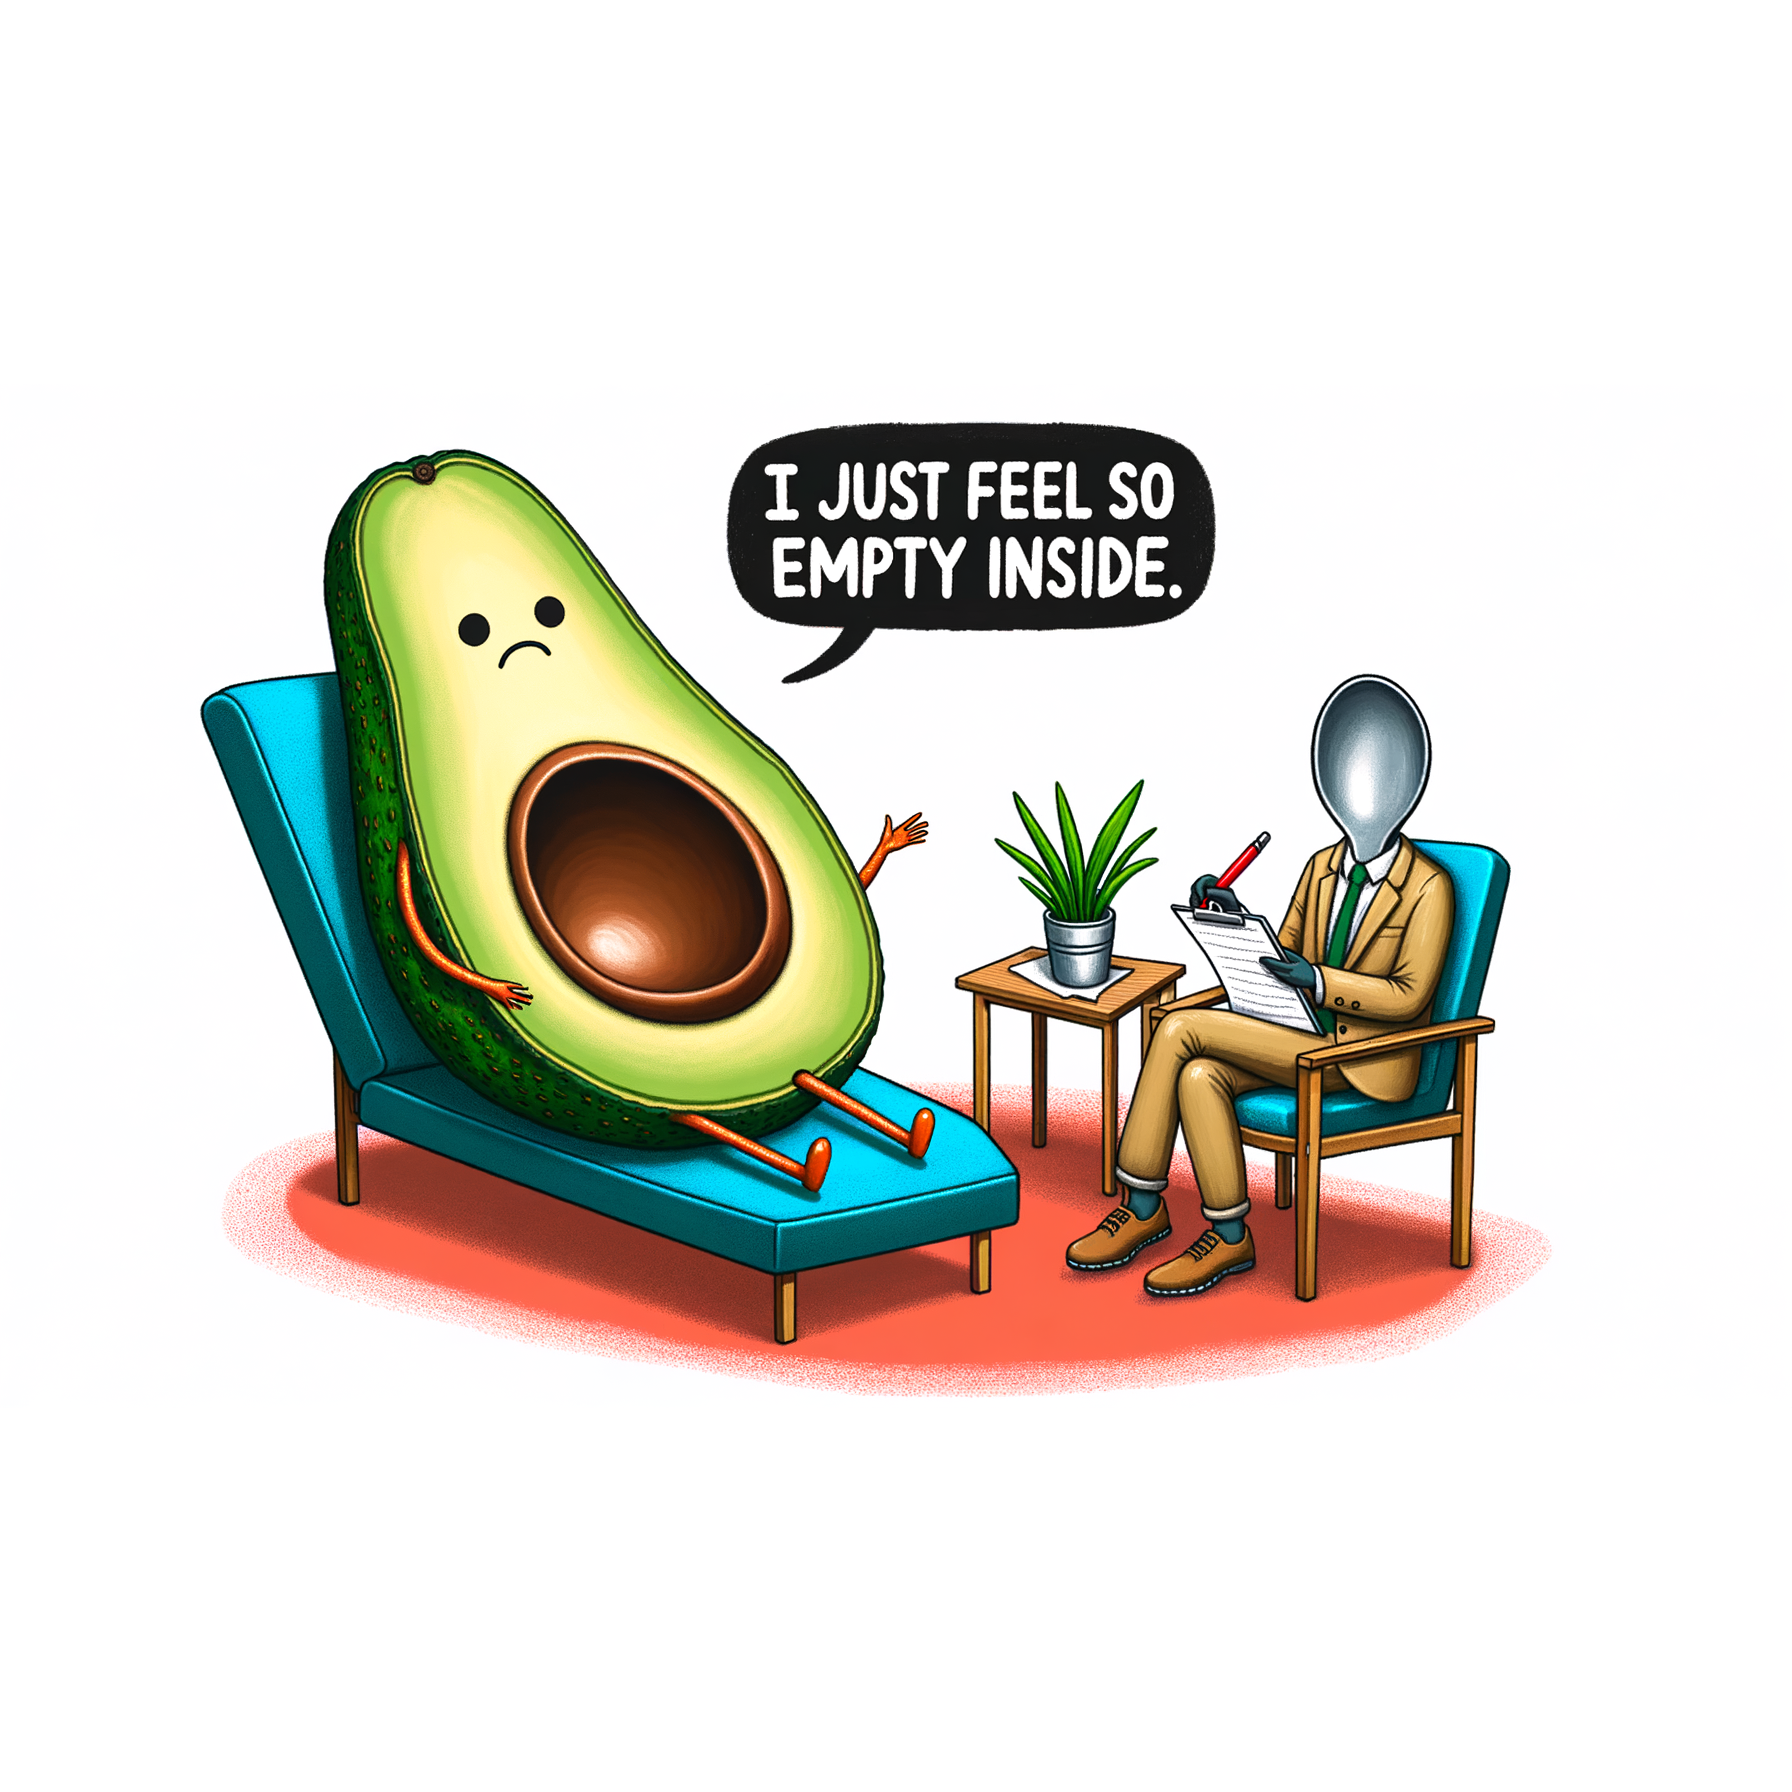
\includegraphics[width=0.32\textwidth]{figs/thesis/dalle3/1.png}
    \hfill
    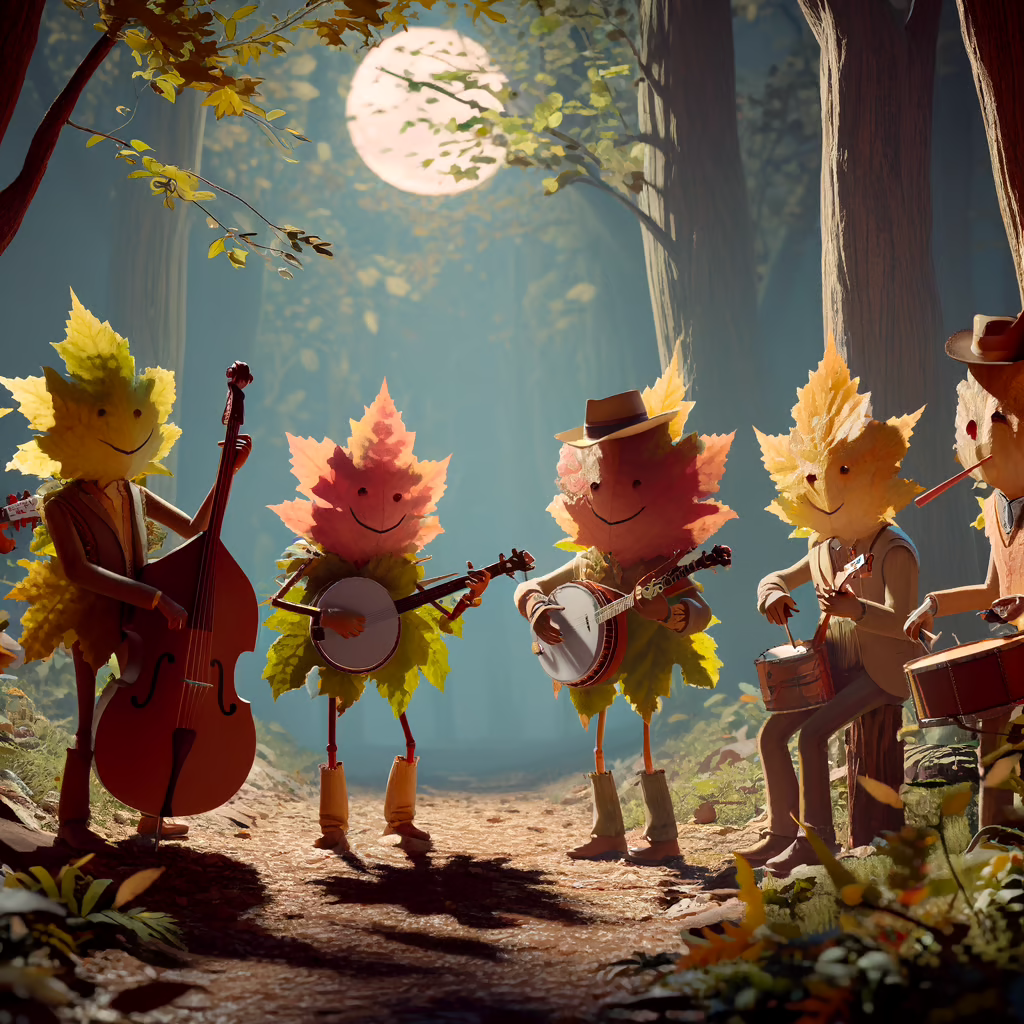
\includegraphics[width=0.32\textwidth]{figs/thesis/dalle3/2.png}
    \hfill
    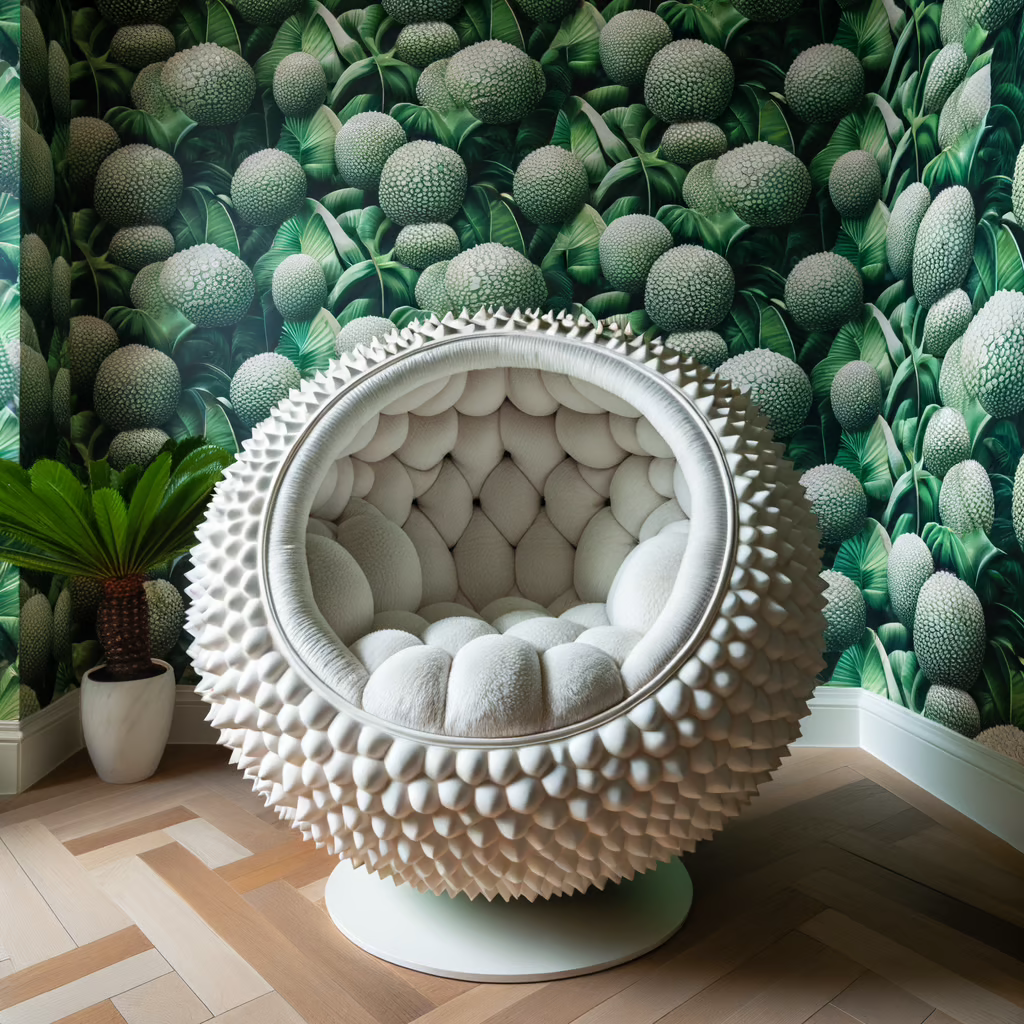
\includegraphics[width=0.32\textwidth]{figs/thesis/dalle3/4.png}
    \caption{Images sampled by diffusion model DALL-E 3~\citep{betker2023improving} given text prompts, from left to right, ``An illustration of an avocado sitting in a therapist's chair, saying 'I just feel so empty inside' with a pit-sized hole in its center. The therapist, a spoon, scribbles notes.''; ``A 2D animation of a folk music band composed of anthropomorphic autumn leaves, each playing traditional bluegrass instruments, amidst a rustic forest setting dappled with the soft light of a harvest moon.''; and ``Photo of a lychee-inspired spherical chair, with a bumpy white exterior and plush interior, set against a tropical wallpaper.''. Reprinted with permission of \citeauthor{betker2023improving}.}
    \label{fig:dalle-3-samples}
    \centering
    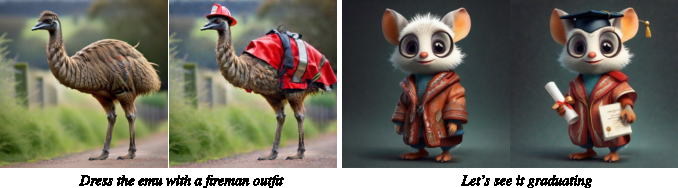
\includegraphics{figs/thesis/emu_edit_examples.pdf}
    \caption{Image edits by a conditional diffusion model, Emu Edit~\citep{sheynin2023emu}. Given an input image (left of each pair) and text prompt, Emu Edit samples an edited image (right of each pair). Reprinted with permission of \citeauthor{sheynin2023emu}.}
    \label{fig:emu-edit-samples}
\end{figure}

\section{Introduction to conditional diffusion models} \label{sec:conditional-diffusion-overview}

In this section we restate the main results from \cref{ch:diffusion} in the conditional diffusion modelling setting. In this setting we will assume that there is a data distribution $p_\text{data}(\rvx, \rvy)$ and we can access $(\rvx, \rvy)$ pairs sampled from it to train our model. Our objective will be to train a model which, given any value of the \textit{conditioning information} $\rvy$, can return a good approximation of the conditional distribution $p_\text{data}(\rvx|\rvy)$, which according to Bayes' rule is equal to $\frac{p_\text{data}(\rvx,\rvy)}{\int p_\text{data}(\rvx,\rvy) \mathrm{d}\rvx}$. The conditioning information can take the form of, for example, an image, a text prompt, a class label, and embedding vector, or a combination of multiple such items.

\paragraph{Training a conditional diffusion model}
To use the methodology from \cref{ch:diffusion} in this setting, we can imagine simply training a different unconditional diffusion model for every possible value of $\rvy$. To do so, we could express the parameters as $\theta[\rvy]$, letting $\theta$ be a data structure that maps from any conditioning information $\rvy$ to the relevant set of diffusion model parameters. Then we could rewrite the diffusion model loss in \cref{eq:general-dm-loss} for a given $\rvy$ as
\begin{align} \label{eq:cond-diffusion-loss-single-y}
    \gL_\text{CDM}(\theta, \rvy) &= \EX_{u(t)q(\rvx_t|\rvx)\pdata(\rvx|\rvy)} \left[ \frac{\lambda^\rvx(t)}{u(t)} 
    \left\| \predx_{\theta[\rvy]}(\rvx_t, t) - \rvx \right\|_2^2 \right]
\end{align}
where we use $\theta[\rvy]$ in place of $\theta$ and sample $\rvx$ from $\pdata(\rvx|\rvy)$ instead of $\rvy$. To train the parameters for all $\rvy$ we may take an expectation of this loss over $\rvy$:
\begin{align} \label{eq:cond-exp-diffusion-loss-all-sigma}
    \gL_\text{CDM}(\theta) &= \EX_{\pdata(\rvy)} \left[ \gL_\text{CDM}(\theta, \rvy) \right] \\
    &= \EX_{u(t)q(\rvx_t|\rvx)\pdata(\rvx, \rvy)} \left[ \frac{\lambda^\rvx(t)}{u(t)} 
    \left\| \predx_{\theta[\rvy]}(\rvx_t, t) - \rvx \right\|_2^2 \right].
\end{align}
Using this objective is feasible if $\rvy$ is discrete and has sufficiently few possible values but if not then it will be inefficient or impossible to train a different set of parameters $\theta[\rvy]$ for every possible value of $\rvy$.

A solution is to share parameters between the neural networks used for different $\rvy$. A standard way to do so is to use the same parameters $\theta$ for each, but pass $\rvy$ as an additional input into the function~\citep{sohn2015learning}. The neural network output $\predx_\theta(\cdot, \rvy, t)$ may then depend on $\rvy$ in an arbitrarily complex way (thanks to the universal approximation theorem~\citep{hornik1989multilayer}) while still being able to share information between different values of $\rvy$ using the single shared set of neural network parameters $\theta$. We will from now on write the learned prediction of $\rvx$ for a conditional diffusion model as $\predx_\theta(\rvx_t, \rvy, t)$. For brevity, we will also expand the definition of the joint distribution $q$ to include $\rvy$ as $q(\rvx,\rvy,\rvx_{t_1},\ldots,\rvx_{t_n}) := q(\rvx_{t_1},\ldots,\rvx_{t_n}|\rvx)\pdata(\rvx,\rvy)$ so the training objective becomes
\begin{align} \label{eq:cond-diffusion-loss}
    \gL_\text{CDM}(\theta) &= \EX_{u(t)q(\rvx_t, \rvx, \rvy)} \left[ \frac{\lambda^\rvx(t)}{u(t)} 
    \left\| \rvx_{\theta}(\rvx_t, \rvy, t) - \rvx \right\|_2^2 \right].
\end{align}
We will similarly write the learned predictions of $\rvx$ and $\epsilon$ as $\predx_{\theta}(\rvx_t, \rvy, t)$ and $\prede_{\theta}(\rvx_t, \rvy, t)$ respectively.
Based on \cref{eq:cond-diffusion-loss-single-y} it is clear that, given some $\rvy$, the diffusion model is learning an approximation of $\pdata(\rvx|\rvy)$. We will therefore denote the distribution it parameterises $p_\theta(\rvx|\rvy)$.

\paragraph{Sampling from a conditional diffusion model}
Other than the new input of $\rvy$, the sampling procedure remains the same. To be explicit, we will nevertheless restate the reverse SDE from \cref{eq:diffusion-edm-sde-approx} in the conditional case:
\begin{align}
    \mathrm{d}\rvx_t = \underbrace{- \frac{1}{2} g(t)^2 \preds_\theta(\rvx_t, \rvy, t) \mathrm{d}t}_{\shortstack{\footnotesize Diffusion ODE \\ \footnotesize similar to \cref{eq:diffusion-ode}}} - \underbrace{\beta(t) \sigma(t)^2 \preds_\theta(\rvx_t, \rvy, t) \mathrm{d}t + \sqrt{2\beta(t)}\sigma(t)\mathrm{d}\bar{\rvw}}_\text{\footnotesize Langevin diffusion}.
\end{align}
The only difference from \cref{ch:diffusion} is that there is an additional input of $\rvy$ to $\preds_\theta$. Recall that this SDE becomes the reverse diffusion ODE from \cref{sec:diffusion-ode} when $\beta(t) = 0$ or the standard reverse diffusion SDE from \cref{sec:diffusion-reverse-sde} when $\beta(t) = \frac{g(t)^2}{2 \sigma(t)^2}$.

\paragraph{Computing likelihoods for conditional diffusion models}
It is possible to compute data likelihoods $p_\theta(\rvx|\rvy)$, or to weight the training objective to lower-bound this likelihood, similarly to the techniques described in \cref{ch:diffusion}. We do not present these results as this is not a focus of this dissertation.

\section{Conditioning on more information improves sample quality} \label{sec:conditioning-on-more-improves-performance}

So far we have mentioned the types of new applications that conditional diffusion models enable as well as introducing the conditional diffusion modelling framework. In this section we make the case that building conditional diffusion models is useful even if the task of interest involves modelling only a single unconditional distribution. We do so by showing that, at least in the image domain, conditional diffusion models often achieve better sample quality than unconditional diffusion models, and then that this insight can be used to make improved \textit{unconditional} generative models that incorporate \textit{conditional} diffusion models.

The better realism of samples from conditional diffusion models versus unconditional diffusion models has previously been noted by \citet{ho2022classifier,bao2022conditional,hu2022self}. Conditional diffusion models have also been observed to work better with few sampling steps~\citep{meng2022distillation}. Furthermore, we will show that sample realism grows with ``how much'' information the diffusion model is conditioned on. To better make this point, we will distinguish between ``strongly-conditional'' generation, where we condition on a high-dimensional feature like a long text prompt, and ``lightly-conditional'' generation, where we condition on a lower dimensional feature like a class label or short text prompt.  As hinted at in \cref{fig:stable-diffusion-example} an image is likely to be more realistic if conditioned on being ``an aerial photograph of a road between green fields'' (strongly-conditional generation) than if it is if simply conditioned on being ``an aerial photograph'' (lightly-conditional generation). Unconditional generation of images will typically lead to even less realism.

\begin{figure}[t]
    \centering
    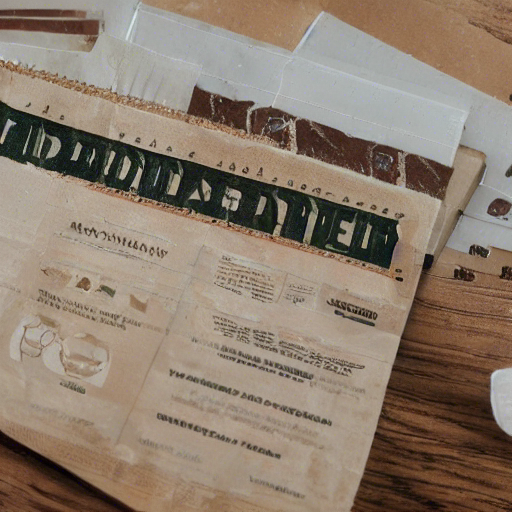
\includegraphics[width=0.3\textwidth]{figs/2sdm/sd_uncond.png}
    \hfill
    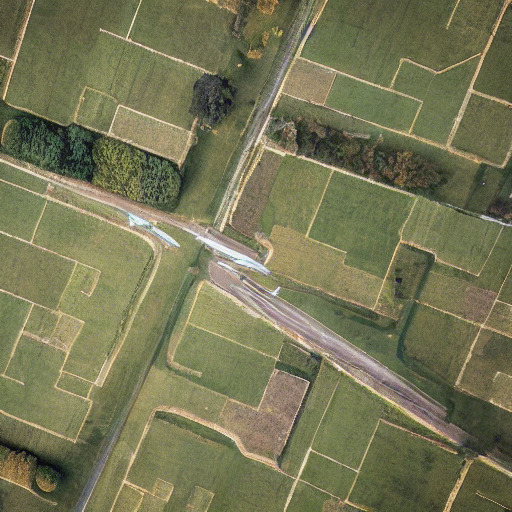
\includegraphics[width=0.3\textwidth]{figs/2sdm/uncond-aerial-photo.jpg}
    \hfill
    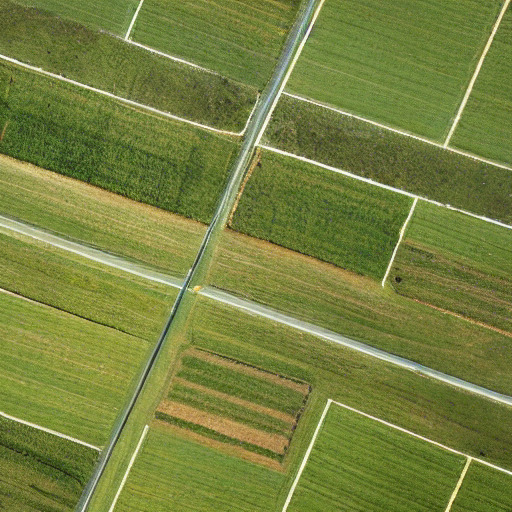
\includegraphics[width=0.3\textwidth]{figs/2sdm/cond-aerial-photo.jpg}
    \caption{Images sampled by Stable Diffusion~\citep{rombach2022high} with the same random seed and three text prompts. \textbf{Left:} Output with an empty text prompt. \textbf{Centre:} Output when prompted to produce ``aerial photography''. \textbf{Right:} Output given a more detailed prompt\protect\footnotemark. Using the more detailed prompt removes the ``smudged'' road artefact visible in the centre image.}
    \label{fig:stable-diffusion-example}
\end{figure}
\footnotetext{We used the prompt ``Aerial photography of a patchwork of small green fields separated by brown dirt tracks between them. A large tarmac road passes through the scene from left to right.''}

\subsection{Analysing conditional vs unconditional diffusion models} \label{sec:2sdm-cond-vs-uncond-dgms}

We will investigate the phenomenon of conditional diffusion models outperforming unconditional diffusion models primarily in the context of conditioning on CLIP (contrastive language-image pre-training)~\citep{radford2021learning} image embeddings. These are embedding vectors encoding high-level, semantically-meaningful information about a given image. The training procedure for such an image embedder is as follows. CLIP jointly trains two neural networks, an image embedder $e_i(\cdot)$ and a text embedder $e_t(\cdot)$, on a large captioned-image dataset. Given an image $\rvx$ and a caption $\rvy$, the training objective encourages the cosine similarity between $e_i(\rvx)$ and $e_t(\rvy)$ to be large if $\rvx$ and $\rvy$ are a matching image-caption pair and small if not.
The image embedder therefore learns to map from an image to a semantically-meaningful embedding capturing any features that may be included in a caption. We use a CLIP image embedder with the ViT-B/32 architecture and weights released by \citet{radford2021learning}. We can visualise the information captured by the CLIP embedding by showing the distribution of images produced by our conditional diffusion model given a single CLIP embedding; see \cref{fig:samples}.

\paragraph{What does it mean to say that conditional diffusion models beat unconditional diffusion models?} A standard procedure to evaluate unconditional diffusion models is to start by sampling a set of $N$ images independently from the model: ${\rvx^{(1)},\ldots,\rvx^{(N)} \sim p_\theta(\cdot)}$. We can then compute the Fr\'echet Inception distance (FID)~\citep{heusel2017gans} between this set and the dataset. If the generative model matches the data distribution well, the FID will be low.
%
For conditional diffusion models the standard procedure has one extra step: we first independently sample ${\rvy^{(1)},\ldots,\rvy^{(N)} \sim \pdata(\cdot)}$. We then sample each image given the corresponding $\rvy^{(i)}$ as ${\rvx^{(i)} \sim p_\theta(\cdot|\rvy^{(i)})}$. 
%
Then, as in the unconditional case, we compute the FID between the set of images $\rvx^{(1)},\ldots,\rvx^{(N)}$ and the dataset, without reference to $\rvy^{(1)},\ldots,\rvy^{(N)}$. Even though it does not measure alignment between $\rvx, \rvy$ pairs, conditional diffusion models beat comparable unconditional diffusion models on this metric in many settings: class-conditional CIFAR-10 generation~\citep{karras2022elucidating}, segmentation-conditional generation~\citep{hu2022self}, or bounding box-conditional generation~\citep{hu2022self}.

\begin{figure}[t]
    \centering
    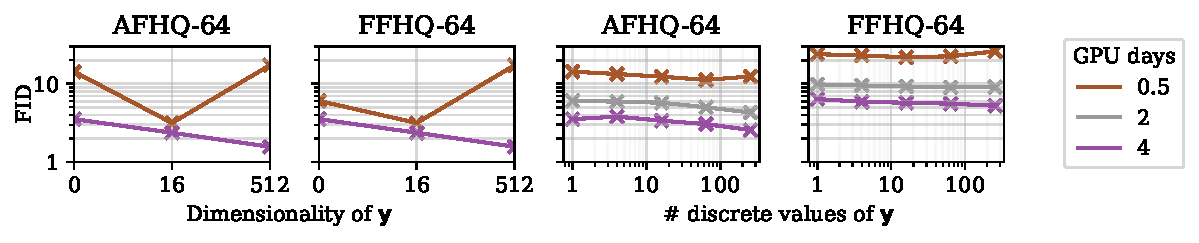
\includegraphics[width=\textwidth]{figs/2sdm/cond-results-vs-nclusters.pdf}
    \caption{Sample quality (measured by FID) versus the dimensionality of conditioning information $\rvy$ for CLIP-conditional image diffusion models on AFHQ~\citep{choi2020stargan} and FFHQ~\citep{karras2018style}. With small training budgets (brown line), it is harmful when $\rvy$ is too informative. With larger training budgets (purple line), it is helpful to make $\rvy$ much more high dimensional.}
    \label{fig:fid-vs-ncomp}
\end{figure}

\paragraph{Why do conditional diffusion models beat unconditional diffusion models?}

Conditional diffusion models ``see'' more data during training than their unconditional counterparts because updates involve $\rvy$ as well as $\rvx$. \citet{bao2022conditional,hu2022self} prove that this is not the sole reason for their successes because the effect holds up even when $\rvy$ is derived from an unconditional dataset through self-supervised learning.
%
To our knowledge, the best explanation for their success is, as stated by \citet{bao2022conditional}, that conditional distributions typically have ``fewer modes and [are] easier to fit than the original data distribution.''

\paragraph{When do conditional diffusion models beat unconditional diffusion models?}
%
We present results in \cref{fig:fid-vs-ncomp} to answer this question. We show FID scores for conditional diffusion models trained to condition on embeddings of varying information content. 
%
We produce $\rvy$ by starting from the CLIP embedding of each image in our dataset and using either principal component analysis to reduce their dimensionality (left two panels) or K-means clustering to discretize them (right two panels)~\citep{hu2022self}.
%
We see that, given a small training budget, it is best to condition on little information. With a larger training budget, performance appears to improve steadily as the dimensionality of $\mathbf{y}$ is expanded. We hypothesize that \textbf{(1)} conditioning on higher-dimensional $\mathbf{y}$ slows down training because it means that points close to any given value of $\mathbf{y}$ will be seen less frequently and $\textbf{(2)}$ with a large enough compute budget, any $\mathbf{y}$ correlated with $\mathbf{x}$ will be useful to condition on.



\subsection{Using conditional diffusion models for unconditional tasks} \label{sec:2sdm-2sdm-method}

The gap in performance between conditional and unconditional diffusion models is problematic. Imagine you need to sample a dataset of synthetic aerial photos.\footnote{ This may be done to, e.g., later train state-of-the-art a classification system~\citep{azizi2023synthetic}.}. A researcher doing so would currently have to either (a) make up a scene description before generating each dataset image, and ensure these cover the entirety of the desired distribution, or (b) accept the inferior image quality gleaned by conditioning just on each image being ``an aerial photograph''.  \Cref{fig:stable-diffusion-example} shows that the difference in quality can be stark.

\begin{figure}[t]
    \centering
    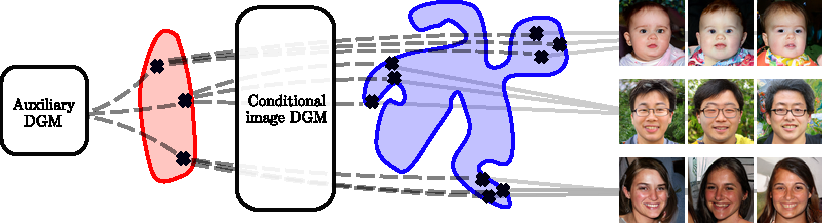
\includegraphics[width=\textwidth]{figs/2sdm/vcdm-diagram.pdf}
    \caption{Visualisation of the procedure to sample from our two-stage diffusion model. First the auxiliary diffusion model samples a CLIP embedding, corresponding to a cross in the space of CLIP embeddings (red) in our illustration. Next, our conditional image model maps from the sampled CLIP embedding to a sampled image, visualized on the image manifold (blue). The distribution over plausible images is complex and multi-modal but becomes simpler when conditioned on a CLIP embedding. On the right we show three rows of sampled images. Within each row, all images are generated given the same CLIP embedding.}
    \label{fig:samples}
\end{figure}
We propose the solution depicted in \cref{fig:samples}. A first ``auxiliary diffusion model'' samples vectors within an embedding space, with any vector describing a particular set of semantic characteristics of an image. The second stage, a ``conditional image diffusion model'', takes such a vector as input and samples an image with these semantic characteristics. The vector embedding is informative, as evidenced by the fact that all images within each row on the right of \cref{fig:samples}, which are all conditioned on the same embedding, look very similar. The conditional image diffusion model therefore inherits all the previously-described advantages of strongly-conditional diffusion models even though our overall generative model is unconditional (or, with the generalisation we will introduce shortly, lightly-conditional). We call the resulting model a Two-Stage Diffusion Model (2SDM).

To describe this model more precisely, we first introduce some notation. Recall that, for unconditional generation, the user does not wish to specify any input to condition on and, for the lightly-conditional setting, any such input is low-dimensional. We will condition our model on any such input in a similar way to the variable that we have been calling $\rvy$ but, to distinguish such additional conditioning input from the CLIP embeddings that we also want to condition on, we will call it $\rva$. Specifically, $\rva$ is a low-dimensional input in the lightly-conditional setting or a null variable in the unconditional setting. For the rest of \cref{sec:conditioning-on-more-improves-performance} we will use $\rvy := e_i(\rvx)$ to refer to a CLIP image embedding. To make this deterministic encoding compatible with a probabilistic generative modelling perspective, we consider a joint distribution $\pdata(\rvx, \rvy, \rva)=\pdata(\rvx, \rva)\delta_{e_i(\rvx)}(\rvy)$, where $\pdata(\rvx, \rva)$ is described by a dataset and $\delta_{e_i(\rvx)}(\rvy)$ is a Dirac conditional distribution enforcing that $\rvy$ is the CLIP embedding of $\rvx$. For the rest of this chapter all distributions denoted with $\pdata$ should be understood as marginals and/or conditionals of this joint distribution, including our target distribution $\pdata(\rvx|\rva)$. 2SDM approximates this target distribution as
%
\begin{align} \label{eq:no-a}
    \pdata(\rvx|\rva) &= \mathbb{E}_{\pdata(\rvy|\rva)} \left[ \pdata(\rvx|\rvy,\rva) \right] \\
    &\approx \mathbb{E}_{p_\phi(\rvy|\rva)} \left[ p_\theta(\rvx|\rvy,\rva) \right] % = p_{\theta,\phi}(\rvx|\rva)
\end{align}
where $p_\theta(\rvx|\rvy,\rva)$ is a conditional image diffusion model modelling $\rvx$ given $\rvy$ and $\rva$ while $p_\phi(\rvy|\rva)$ is a second diffusion model modelling the CLIP embeddings $\rvy$ given $\rva$. We can sample from this distribution by sampling $\rvy\sim p_\phi(\cdot|\rva)$ and then leveraging the conditional image diffusion model to sample $\rvx \sim p_\theta(\cdot|\rvy,\rva)$ We then return $\rvx$ and make no further use of $\rvy$.
%
From now on we will call $p_\theta(\rvx|\rvy,\rva)$ the \textit{conditional image model} and $p_\phi(\rvy|\rva)$ the \textit{auxiliary model}. In our experiments the auxiliary model uses a small architecture relative to the conditional image model and so adds little extra cost.\footnote{For our ImageNet experiments, sampling from our auxiliary model takes 35ms per batch item. Sampling from our image model takes 862ms and so 2SDM has inference time only $4\%$ greater than our baselines.}


\paragraph{Auxiliary model}
Our auxiliary model is a conditional diffusion model targeting $\pdata(\rvy|\rva)$, where $\rvy$ is a 512-dimensional CLIP embedding. Following \cref{eq:cond-diffusion-loss}, we train it by minimising
\begin{equation}
\label{eq:auxiliary-model-objective}
    \mathbb{E}_{u(\sigma)q(\rvy_\sigma|\rvy)\pdata(\rvy,\rva)} \left[ \frac{\lambda^\rvx(\sigma)}{u(\sigma)} \lvert\lvert \rvy - \hat{\rvy}_\theta(\rvy_\sigma, \rva, \sigma) \rvert\rvert_2^2 \right]
\end{equation}
where $q(\rvy_\sigma|\rvy) = \gN(\rvy_\sigma; \rvy, \sigma^2\mI)$. We use a variance-exploding diffusion process following \citet{karras2022elucidating}, and also match their diffusion process hyperparameters, including $\lambda^\rvx$ and $u(\sigma)$ (which is a continuous distribution), and use their proposed Heun sampler. We follow the architectural choice of \citet{ramesh2022hierarchical} and use a diffusion model with a transformer architecture. It takes as input a series of 512-dimensional input tokens: an embedding of $\sigma$; an embedding of $\rva$ if this is not null; an embedding of $\rvy_\sigma$; and a learned query. These are passed through six transformer layers and then the output corresponding to the learned query token is used as the output. Like \citet{ramesh2022hierarchical}, we parameterise the diffusion model to directly output a mean-squared error estimate of $\rvy$.
%
On AFHQ and FFHQ we find that data augmentation is helpful to prevent the auxiliary model overfitting. We perform augmentations (including rotation, flipping and color jitter) in image space and feed the augmented image through $e_i(\cdot)$ to obtain an augmented CLIP embedding. Following \citet{karras2022elucidating}, we pass a label describing the augmentation into the transformer as an additional input token so that we can condition on there being no augmentation at test-time.


\paragraph{Conditional image model}
Including the additional conditioning input $\rva$, the conditional image model's training objective is
\begin{equation}
\label{eq:conditional-image-model-objective}
    \mathbb{E}_{u(\sigma)q(\rvx_\sigma|\rvx)\pdata(\rvx,\rvy,\rva)} \left[ \frac{\lambda^\rvx(\sigma)}{u(\sigma)} \lvert\lvert \rvx - \predx_\theta(\rvx_\sigma, \rvy \oplus \rva, \sigma) \rvert\rvert_2^2 \right].
\end{equation}
where $\rvy \oplus \rva$ is the concatenation of $\rvy$ and $\rva$ to form a single vector which the image model is conditioned on. As with the auxiliary model, we use a variance-exploding diffusion process with the hyperparameters and Heun solver of \citet{karras2022elucidating}. For AFHQ and FFHQ, we use the U-Net architecture originally proposed by \citet{song2020score}. For ImageNet, we use the slightly larger U-Net architecture proposed by \citet{dhariwal2021diffusion}. We match the data augmentation scheme to be the same as that of \citet{karras2022elucidating} on each dataset. There are established conditional variants of both architectures~\citep{dhariwal2021diffusion,karras2022elucidating} that add a learned linear projection to the embedding of the noise standard deviation $\sigma$.  We use the same technique to incorporate the concatenated conditioning inputs $\rvy\oplus\rva$.

\subsection{Two-stage diffusion improves over standard diffusion} \label{sec:2sdm-experiments}


\begin{table}[t]
\centering
\small
\caption{Comparison of a standard diffusion model (EDM) with our two-stage approach (2SDM) on a suite of image-generation metrics. Best performance for each metric and dataset is shown in bold. Higher is better for metrics marked $\uparrow$; lower is better for $\downarrow$. Results reported for EDM on FFHQ and AFHQ are computed with the pretrained checkpoints released by \citet{karras2022elucidating}. Results reported for 2SDM on FFHQ are with finetuning from this pretrained checkpoint. All others are trained from scratch.}
\begin{tabular}{lcccccc}
\toprule
 \multirow{2}{*}{Dataset} & \multirow{2}{*}{Method} & \multirow{2}{*}{\shortstack{Inception\\Score $\uparrow$}} & \multirow{2}{*}{Precision $\uparrow$} & \multirow{2}{*}{Recall $\uparrow$} & \multirow{2}{*}{FID $\downarrow$} & \multirow{2}{*}{sFID $\downarrow$} \\
 & & & & & & \\
\midrule
\multirow{2}{*}{AFHQ-64} & 2SDM & $\mathbf{10.00}$ & $\mathbf{0.844}$ & $\mathbf{0.619}$ & $\mathbf{1.56}$ & $13.7$ \\
 & EDM & $8.91$ & $0.752$ & $0.614$ & $2.04$ & $13.7$ \\
\midrule
\multirow{2}{*}{FFHQ-64} & 2SDM & $\mathbf{3.47}$ & $\mathbf{0.721}$ & $\mathbf{0.697}$ & $\mathbf{2.32}$ & $4.98$ \\
 & EDM & $3.33$ & $0.697$ & $0.569$ & $2.46$ & $\mathbf{4.90}$ \\
\midrule
\multirow{2}{*}{\shortstack[l]{Class-cond. \\ ImageNet-64}} & 2SDM & $\mathbf{17.3}$ & $\mathbf{0.541}$ & $\mathbf{0.573}$ & $\mathbf{17.4}$ & $\mathbf{4.63}$ \\
 & EDM & $13.6$ & $0.530$ & $0.532$ & $25.4$ & $6.50$ \\
\midrule
\multirow{2}{*}{\shortstack[l]{Uncond. \\ ImageNet-64}} & 2SDM & $\mathbf{15.6}$ & $\mathbf{0.614}$ & $\mathbf{0.526}$ & $\mathbf{21.0}$ & $\mathbf{5.59}$ \\
 & EDM & $11.3$ & $0.523$ & $0.524$ & $35.1$ & $9.14$ \\
 \midrule
\multirow{2}{*}{\shortstack[l]{Class-cond. latent \\ ImageNet-256}} & 2SDM & $\mathbf{52.1}$ & $\mathbf{0.590}$ & $0.603$ & $\mathbf{24.3}$ & $\mathbf{7.36}$ \\
 & EDM & $40.4$ & $0.532$ & $\mathbf{0.610}$ & $34.2$ & $9.59$ \\
\end{tabular}
\label{tab:2sdm-many-metrics}
\end{table}

\paragraph{Experimental setup and results overview}

We perform experiments in five settings: unconditional AFHQ modelling at $64\times64$ resolution~\citep{choi2020stargan}; unconditional FFHQ modelling at $64\times64$ resolution~\citep{karras2018style}; class-conditional ImageNet modelling at $64\times64$ resolution~\citep{deng2009imagenet}; unconditional ImageNet modelling at $64\times64$ resolution; and finally class-conditional latent ImageNet modelling in which we model a compressed $32\times32\times4$ representation of a $256\times256$ image as we will describe shortly. In every setting, we compare against EDM~\citep{karras2022elucidating}, a standard DM directly modelling $\pdata(\rvx|\rva)$, with an identical architecture to 2SDM's conditional image model. We also match the training compute of our conditional image model with that of EDM in every case. Auxiliary models for each setting are trained for one day on a single V100 GPU so add little additional cost. We report the metrics achieved by EDM and 2SDM on each setting in \cref{tab:2sdm-many-metrics} before giving more detail and analysis. The Inception Score~\citep{salimans2016improved,barratt2018note} in \cref{tab:2sdm-many-metrics} measures the diversity of the output from an image classifier when run on sampled images. The Precision and Recall metrics~\citep{kynkaanniemi2019improved} estimate, roughly speaking, the proportion of generated images that lie on the data manifold (Precision) and the proportion of dataset images that can be found within the manifold of generated images (Recall). The FID approximates the distance between the distribution of embeddings of dataset images and that of embeddings of generated images. The sFID is similar but uses an embedding with more spatial information. 2SDM outperforms EDM on 22 of the 25 metric-dataset combinations, and is outperformed on only 2.


\begin{figure*}[t]
    \centering
    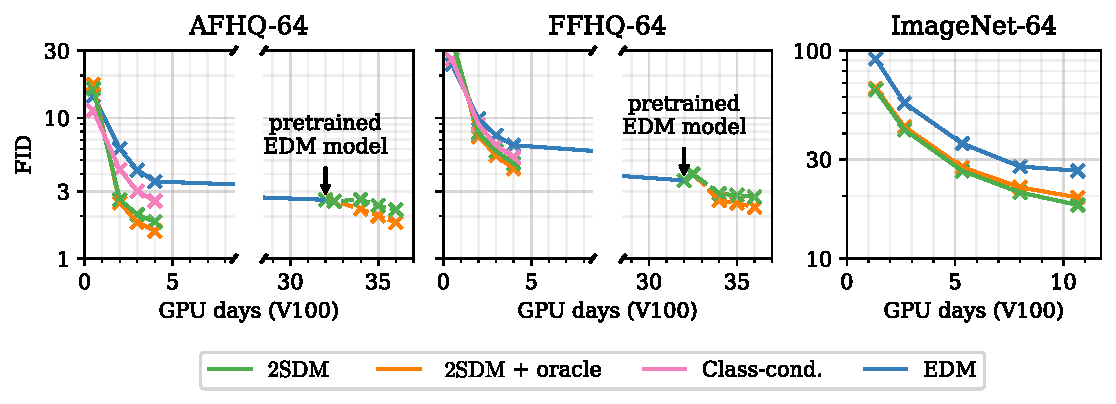
\includegraphics[width=\textwidth]{figs/2sdm/cond-results-1.pdf}
    \caption{FID throughout training for our method and baselines on AFHQ, FFHQ, and class-conditional ImageNet-64. We show results for each method trained from scratch and, on AFHQ and FFHQ, for finetuning a pretrained EDM model (which was trained for the equivalent of 32 GPU days). 2SDM quickly outperforms EDM when trained from scratch and quickly improves on the pretrained model when used for finetuning.}
    \label{fig:fid_vs_training}
\end{figure*}


\paragraph{Details and analysis for AFHQ, FFHQ, and ImageNet-64}
On AFHQ and FFHQ, we match the EDM parameters to those of \citet{karras2022elucidating}. On ImageNet-64, we have a smaller training budget and so decrease the batch size to 128 and the learning rate to $1\times10^{-4}$. For simplicity we match 2SDM to use the same learning rate and batch size. \cref{fig:fid_vs_training} reports the FID throughout the training of the conditional image diffusion model (or image DM baseline) for AFHQ, FFHQ, and class-conditional ImageNet-64.\footnote{Each FID in \cref{fig:fid_vs_training} is estimated using $20\,000$ images, each sampled with the SDE solver proposed by \citet{karras2022elucidating} using 40 steps, $S_\text{churn}=50$, $S_\text{noise}=1.007$, and other parameters set to their default values. Our other reported FID scores use $50\,000$ samples, as is standard, and the same sampler hyperparameters.}  We consider training the conditional image model from scratch (for up to 4 GPU days on AFHQ and FFHQ, or up to 11 GPU days on ImageNet-64), and see that it improves upon our EDM baseline for any training budgets over 1-2 GPU days. For AFHQ, this improvement is so substantial that 2SDM's FID after two GPU days is better than that of the pretrained EDM model released by \citet{karras2022elucidating}, which was trained for the equivalent of 32 V100 GPU days. In addition to training from scratch, on AFHQ and FFHQ we consider initializing 2SDM's training from the pretrained EDM checkpoints. To do so, we simply add a learnable linear projection of the CLIP embedding and initialize its weights to zero. We see that this allows for a fast and significant improvement in FID over the baseline in each case. We note, though, that training 2SDM from scratch for 4 GPU days outperforms 4 GPU days of finetuning on AFHQ and so recommend training 2SDM from scratch when sufficient compute is available.

\Cref{fig:fid_vs_training} also compares against ``2SDM + oracle'', which is a supposed upper bound on 2SDM's performance given by sampling a CLIP image embedding from an oracle (in practice, the dataset) and then using 2SDM's conditional image model to sample an image conditioned on it. It therefore describes the performance that 2SDM would achieve with a perfect auxiliary model. On AFHQ-64, 2SDM with an oracle achieves a FID $56\%$ lower than EDM. Without an oracle, 2SDM still achieves a FID $48\%$ lower than 2SDM. We therefore say that 2SDM yields an improvement $87\%$ as large as can be gleaned by using a purely conditional DM. Similarly for FFHQ, 2SDM obtains an improvement $81\%$ as large as is possible with a purely conditional DM.\footnote{Our calculation of these numbers is as follows. On AFHQ-64, 2SDM with an oracle achieved a FID of $1.57$, a $56\%$ improvement on the FID of $3.53$ achieved with EDM. 2SDM without an oracle achieved a FID of $1.83$, a $48\%$ improvement on $3.53$. This is $87\%$ as large as the improvement achieved with an oracle. Similarly on FFHQ-64, 2SDM with an oracle achieved a FID of $4.35$, a $32\%$ improvement on the FID of $6.39$ achieved with EDM. 2SDM without an oracle achieved a FID of $4.73$, a $26\%$ improvement on $6.39$. This is $81\%$ as large as the improvement achieved with an oracle.} We can therefore say that our cheaply-trained auxiliary model is good enough to allow us to capture the majority of the benefits of conditional generation for the unconditional generation task. Intriguingly,
 on ImageNet-64, 2SDM achieves better FID \textit{without} an oracle. This suggests that imperfections in the distribution
learned by the auxiliary model improve the visual quality of the generated images. We observed this trend consistently on ImageNet, and believe that characterising exactly when and why it occurs is an intriguing direction for future work.

Finally, \cref{fig:fid_vs_training} also compares against ``Class-cond'', which is an ablation of 2SDM in which we replace the CLIP embedding $\rvy$ with a single discrete label obtained by K-means clustering of the CLIP embedding (as on the right of \cref{fig:fid-vs-ncomp}). For unconditional generation tasks, we can then replace our auxiliary model with a simple categorical distribution modelling $\pdata(\rvy|\rva)=\pdata(\rvy)$ similarly to \citet{hu2022self}, simplifying the generative procedure. We see that this baseline is outperformed by 2SDM, justifying our choice to use a continuous $\mathbf{y}$.

\begin{figure}[t]
    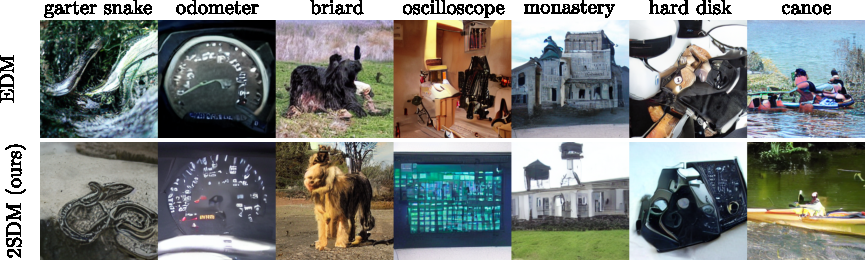
\includegraphics[width=\textwidth]{figs/2sdm/2SDM-main-fig.pdf}
    \caption{Comparison of class-conditional ImageNet-256 samples from our two-stage diffusion model, 2SDM, and from a diffusion model baseline, EDM~\citep{karras2022elucidating}. Both are trained for 12 GPU days. Samples within the same column are generated with the same random seed and class label.}
    \label{fig:latent-imagenet-samples}
\end{figure}

\paragraph{Details and analysis for ImageNet-256}
We combine 2SDM and the latent diffusion modelling framework~\citep{rombach2022high} on the ImageNet-256 dataset as follows. We take the pretrained encoder and decoder of the Stable Diffusion auto-encoder released by \citet{rombach2022high}. We feed $256\times256\times3$ dataset images through the VAE encoder to create $64\times64\times4$ tensors, which we use as the training targets $\rvx$ for our conditional image model. The training targets for the CLIP embeddings $\rvy$ are created by embedding the $256\times256\times3$ images with the standard CLIP image embedder. We use the ImageNet class labels as additional inputs $\rva$. At test time, we take $\rva$ as an input; we then sample $\rvy$ given $\rva$ from our auxiliary model; we then sample $\rvx$ given $\rvy$ and $\rva$ from our conditional image model; we finally use the Stable Diffusion VAE decoder to produce an image given $\rvx$. Samples from this version of 2SDM, as well as our EDM baseline operating in the same latent space, are shown in \cref{fig:latent-imagenet-samples}. While the compute used for each (12 GPU days) is far from that of the state-of-the-art for this dataset, the samples from 2SDM are noticeably better, supporting the FID scores in \cref{tab:2sdm-many-metrics}.

\paragraph{Comparison of relative improvements between tasks}
In terms of FID, and for the networks trained from scratch and matched for training compute, the percentage improvement of 2SDM over EDM is $48.2\%$ on AFHQ-64; $26.0\%$ on FFHQ-64; $31.5\%$ on class-conditional ImageNet-64; $40.2\%$ on unconditional ImageNet-64; and $28.9\%$ on class-conditional ImageNet-256. While these are all substantial improvements, we point out two comparisons in particular. 

First, the gain from using 2SDM on unconditional ImageNet-64 ($40.2\%$) is greater than that on class-conditional modelling of the same dataset ($31.5\%$). This supports our argument that two-stage diffusion techniques like 2SDM can have even greater impact in unconditional (or lightly-conditional) generation than in the text-conditional (or strongly-conditional) setting in which they were originally introduced with unCLIP~\citep{ramesh2022hierarchical}.  Noting that the class label already contains some of the information stored in a CLIP embedding, this finding also fits with our discussion of the effects of conditioning in \cref{sec:2sdm-cond-vs-uncond-dgms}. In particular, our discussion in \cref{sec:2sdm-cond-vs-uncond-dgms} suggests that the performance of an image model conditioned on just a class label (EDM on class-cond. ImageNet) should be somewhere in between that of an unconditional image model (EDM on uncond. ImageNet) and that of a CLIP-conditional image model (2SDM, assuming the auxiliary model is good), and we find that this is true.

Second, the $28.9\%$ improvement in performance for the latent diffusion model on ImageNet-256 is only slightly less than the $31.5\%$ improvement for pixel-space diffusion on class-conditional ImageNet-64. This supports that the 2SDM approach of conditioning on high-level but low-dimensional embeddings is readily combined with the widely-used latent diffusion framework, which models the data via a relatively high-dimensional representation.

\paragraph{Inference speed}
Sampling from 2SDM does impose a small additional cost relative to EDM, since we must begin by sampling from the auxiliary model. In all experiments, when we use 40 diffusion steps, sampling from our auxiliary model takes 8.8s with batch size 256. This corresponds to 35ms per batch item. Our conditional image model and our EDM baseline use identical architectures (other than the projection of $\rvy$) and we could not detect a difference between their sampling times which were 862ms per batch item on our ImageNet architecture and 789ms per batch item on our AFHQ and FFHQ architecture. This means that the increase in time due to using 2SDM instead of EDM is less than $4\%$. Furthermore, we can negate this increase by using two less sampling steps for the conditional image model. We show in \cref{supp:conditional-diffusion} that this lets us make 2SDM faster than EDM with almost no effect on sample quality.


\subsection{Perspectives on two-stage diffusion}
\paragraph{UnCLIP} \label{sec:unclip}
UnCLIP~\citep{ramesh2022hierarchical} uses the following text-to-image procedure: given a text prompt, it is embedded by a CLIP text embedder. A diffusion model then samples a plausible CLIP image embedding with high cosine similarity to this text image embedding. Finally, a conditional image diffusion model samples an image conditioned on CLIP image embedding and text prompt. This is described as ``inverting'' the CLIP embedder framework to map from image to text, hence the name unCLIP. Given our discussion of the benefits of conditioning the diffusion model on as much information as possible, it makes sense that unCLIP provides a benefit as long as the combination of text prompt and CLIP image embedding contains ``more'' information than the text prompt alone, which will always be the case. They also imply that the disparity is even larger if we compare the CLIP-conditional generative model with an unconditional generative model (i.e. one conditioned on zero bits of information). The unCLIP approach can therefore be expected to provide larger benefits for unconditional (or lightly-conditional) generation than for the text-conditional setting in which it was developed. This is supported by our findings with 2SDM which show bigger benefits over EDM for unconditional generation than for class-conditional generation.

\paragraph{Intermediate variables in diffusion models}~
 The proposed model takes inspiration from \citet{weilbach2023graphically}, % who use diffusion models to perform approximate inference in graphical models. They 
who show improved performance in various approximate inference settings by modelling problem-specific auxiliary variables (like $\rvy$) in addition to the variables of interest ($\rvx$) and observed variables ($\rva$). We apply these techniques to the image domain and incorporate pretrained CLIP embedders to obtain auxiliary variables. 

\paragraph{Latent diffusion}~
2SDM also relates to methods which perform diffusion in a learned latent space~\citep{rombach2022high}: our auxiliary model $p_\phi(\rvy|\rva)$ is analogous to a ``prior'' in a latent space and our conditional image model $p_\theta(\rvx|\rva,\rvy)$ to a ``decoder'' Such methods typically use a near-deterministic decoder and so their latent variables must summarise all information about the image. Our conditional diffusion model decoder, on the other hand, is a diffusion model that can generate realistic images even if little information is stored in $\rvy$. This means that 2SDM provides an additional degree of freedom in terms of what to store. Furthermore, as we showed in \cref{sec:2sdm-experiments}, 2SDM can be fruitfully combined with latent diffusion.

\paragraph{Self-supervised representations}~
\citet{bao2022conditional,hu2022self} both use self-supervised learning to obtain auxiliary variables and then training a diffusion model $p(\rvx|\rva)$. However, they do not model $\rva$ and therefore are not able to sample $\rvx$ without an oracle that can provide $\rva$. Their success when given an oracle, however, provides reason to believe that our approach is likely to yield benefits even if the embedder that produces $\rva$ is obtained through self-supervised learning and without access to additional (or multi-modal) data as our CLIP embedder was trained with.

\paragraph{Integrating additional data}~
Our method can be understood as a means to leverage the ``world knowledge'' inside a CLIP embedder for improved performance on the image generation task. Another way in which additional knowledge, or data, could be leveraged is by training a multi-headed diffusion model which simultaneously approximates the score function and makes predictions of side information like class labels. \citet{deja2023learning} propose a method for doing so but do not demonstrate improved performance on the unconditional generation task.

\subsection{Final discussion of two-stage diffusion}
In this section we have demonstrated that conditional diffusion models can outperform unconditional diffusion models in terms of sample realism in the image domain, and that we can leverage this insight to build improved unconditional and lightly-conditional DGMs. This provides motivation for our work on conditional generation in addition to the new systems that are enabled by the capability to do conditional generation. 

We note, though, that a massive unexplored design space remains after the results we have presented on 2SDM. For pedagogical purposes we intentionally kept 2SDM simple, using known diffusion architectures and objectives. It is likely that optimising these design choices for the lightly-conditional 2SDM use-case would improve performance. In addition, there are almost certainly more useful quantities that we could condition on than CLIP embeddings. 
\citet{bao2022conditional,hu2022self} have shown that self-supervised learning techniques provide a promising avenue for obtaining useful ``latent'' representations. Exactly the properties that an embedding should have to be beneficial for techiques like 2SDM is another open question that is ripe for future work to tackle. Such a line of work may also fix one limitation of 2SDM, namely that it relies on the availability of a pretrained CLIP embedder. While this is freely available for natural images, it could be a barrier to other applications. Improvements may also be gleaned by conditioning on multiple quantities, or ``chaining'' a series of conditional diffusion models together. An alternative direction is to simplify 2SDM's architecture by, for example, learning a single diffusion model over the joint space of $\rvx$ and $\rvy$ instead of generating them sequentially.

\section{Other methods for conditional sampling} \label{sec:other-methods-for-conditional-sampling}
So far we have described how diffusion models can be trained explicitly as conditional models, and the technique we described for doing so will form the foundation of this thesis. Another class of methods, though, which we will use in \cref{ch:tddm}, make it possible to draw conditional samples from \textit{unconditional} diffusion models. In particular, in this section we will describe the replacement method, reconstruction guidance, and classifier guidance~\citep{song2020score,kadkhodaie2020solving,mittal2021symbolic,ho2022video}. We end the section by discussing classifier-free guidance, which builds on these techniques to sometimes improve the sample quality attainable with a conditional diffusion model.

\subsection{Replacement method}
We first describe a method proposed by \citet{song2020score} to use an unconditional diffusion model for imputation; that is, to sample the values of a subset of the dimensions of $\rvx$ conditioned on the values of the other dimensions. Recalling our notation from the introduction, let $\gY$ be a list containing the indices of any dimension whose value is observed and let $\rvy = \rvx[\gY]$ be the corresponding list of observed values.
Similarly, let $\rvx_t[\gY]$ denote all the values in $\rvx_t$ corresponding to observed values in $\rvx$.
\citet{song2020score} suggest modifying $\rvx_t[\gY]$ at each integration step while sampling from the reverse SDE. In particular, they modify the values of $\rvx_t$ at indices $\gY$ by replacing them with samples from $q(\rvx_t[\gY] ~|~ \rvx[\gY] )$, i.e. with the observed values corrupted by time-dependent noise. This method is sometimes referred to as the ``replacement method'' as it simply continuously replaces some dimensions of $\rvx_t$ with new values that tend towards their observed values as $t$ tends to zero.

\subsection{Conditioning on any linear projection}
The replacement method described above is applicable more generally in that, as well as being used to condition on the values of any subset of the dimensions in $\rvx$, it can be used to condition on the value of any linear projections of $\rvx$. That is, given an unconditional diffusion model outputting $\preds_\theta(\rvx_t, t)$ to approximate the score function $\nabla_{\rvx_t} \log q(\rvx_t)$, we can draw samples from an approximation of $\pdata(\rvx|\rvy)$ where $\rvy:=\mA\rvx$ for any projection matrix $\mA \in \mathbb{R}^{m \times n}$ with number of columns $n$ matching the dimensionality of $\rvx$ and number of rows $m \leq n$ matching the dimensionality of $\rvy$.

To do so, \citet{song2020score} point out that it is always possible to rotate the data given $\mA$ such that some dimensions are fully observed and the remainder are fully unobserved. At this point, the replacement method can be used. To perform the rotation, we will assume that the rows of $\mA$ are of unit magnitude and are orthogonal to eachother.\footnote{We can do so without loss of generality since it is possible to transform any $\mA$ to meet these conditions without changing the information stored in $\rvy$ using the Gram-Schmidt process.} We then add more basis vectors to create a rotation matrix $\mR \in \mathbb{R}^{n \times n}$ such that its first $m$ rows are the rows of $\mA$. We can then transform $\rvx$ into $\hat{\rvx} := \mR \rvx$. The first $m$ dimensions of $\hat{\rvx}$ have observed values $\rvy := \mA\rvx$ and the remaining $n-m$ are to be sampled with the diffusion model. This means that we can use the replacement method, as described previously, to sample $\hat{\rvx}$ as long as we can compute the score $\nabla_{\predx_t} \log q(\predx_t)$. As shown by \citet{song2020score}, this is simple to compute as $\nabla_{\predx_t} \log q(\predx_t) = \mR \nabla_{\rvx_t} \log q(\rvx_t) \approx \mR \preds_\theta(\rvx_t, t) = \mR \preds_\theta(\mR^\top \predx_t, t)$. Once we have sampled $\hat{\rvx}$ given $\rvy$, we can transform it into the original data space as $\rvx = \mR^\top \hat{\rvx}$.

\subsection{Reconstruction guidance} \label{sec:reconstruction-guidance}
\citet{ho2022video} point out that the replacement method is not a perfect approximation of the desired conditional distribution because it uses an approximation of the score function $\nabla_{\rvx_t} \log q(\rvx_t)$ instead of the conditional score function $\nabla_{\rvx_t} \log q(\rvx_t~|~\rvx[\gY])$. While $\rvx_t$ does contain some information about $\rvx[\gY]$ thanks to $\rvx_t[\gY]$ being sampled from $q(\cdot ~|~ \rvx[\gY])$, there is still information lost due to the noise in $q(\rvx_t[\gY] ~|~ \rvx[\gY])$ and so these two score functions are not the same. \citet{ho2022video} derive an approximation by breaking the desired conditional score function into two terms as
\begin{align}
    \nabla_{\rvx_t} \log q(\rvx_t~|~\rvx[\gY]) &= \nabla_{\rvx_t} \log \frac{q(\rvx_t, \rvx[\gY])}{q(\rvx[\gY])}\\
    &= \nabla_{\rvx_t} \log \left( q(\rvx_t) q(\rvx[\gY]~|~\rvx_t) \right) - \underbrace{\nabla_{\rvx_t} \log q(\rvx[\gY])}_{=0} \\
    &= \underbrace{\nabla_{\rvx_t} \log q(\rvx_t)}_\text{estimated by diffusion model} + \underbrace{\nabla_{\rvx_t} \log q(\rvx[\gY]~|~\rvx_t)}_\text{intractable}. \label{eq:approx-score-function-recon-guidance}
\end{align}
The final term of \cref{eq:approx-score-function-recon-guidance} is unfortunately intractable, but \citet{ho2022video} suggest approximating it by assuming that $q(\rvx[\gY]~|~\rvx_t)$ is a Gaussian whose mean is the neural network's prediction of $\rvx$ for observed dimensions, $\predx_\theta(\rvx_t, t)[\gY]$, and with element-wise standard deviation $\sigma(t) / \alpha(t)$. This leads to the score function
\begin{align}
    \nabla_{\rvx_t} \log q(\rvx[\gY]~|~\rvx_t) &\approx \nabla_{\rvx_t} \log \gN \left( \rvx[\gY]; \predx_\theta(\rvx_t, t)[\gY], \frac{\sigma(t)^2}{\alpha(t)^2} \mI \right) \\
    &= -\frac{\alpha(t)^2}{2\sigma(t)^2} \nabla_{\rvx_t} \left\| \rvx[\gY] - \predx_\theta(\rvx_t, t)[\gY] \right\|_2^2.
\end{align}
\citet{ho2022video} suggest adding a scaling factor $w$ to enable control of how ``strongly conditioned'' the output is on $\rvy$ and so finally estimate the score function as 
\begin{align}
    \nabla_{\rvx_t} \log q(\rvx_t~|~\rvx[\gY]) &= \nabla_{\rvx_t} \log q(\rvx_t) - \frac{w \cdot \alpha(t)^2}{2\sigma(t)^2} \nabla_{\rvx_t} \left\| \rvx[\gY] - \predx_\theta(\rvx_t, t)[\gY] \right\|_2^2 . \label{eq:recon-guidance-score-function}
\end{align}
Other than using this updated score function to take each step, reconstruction guidance has all other steps identical to the replacement method described above. Note, though, that computing the second term in \cref{eq:recon-guidance-score-function} requires differentiating through the neural network, so reconstruction guidance is more computationally expensive than the replacement method. 

\subsection{Classifier guidance}
Classifier guidance~\citep{song2020score} applies when the conditioning information is a discrete label. It enables conditional sampling from a unconditional diffusion model, but does require one model specifically trained for the conditioning task: a classifier $p_\theta(\rvy|\rvx_t) \approx q(\rvy|\rvx_t)$ that estimates the probability of the discrete label $\rvy$ given noisy data $\rvx_t$. For e.g. an image diffusion model, this classifier might have a similar architecture to a standard image classifier but it should take noisy images as input and additionally should receive the timestep describing how noisy the input image is. We can make use of the classifier if we decompose the conditional score function as
\begin{align}
    \nabla_{\rvx_t} \log q(\rvx_t|\rvy) &= \nabla_{\rvx_t} \log \frac{q(\rvx_t)q(\rvy|\rvx_t)}{q(\rvy)} \label{eq:cg-derivation-line1} \\
    &= \nabla_{\rvx_t} \log \left( q(\rvx_t) q(\rvy|\rvx_t) \right) - \underbrace{\nabla_{\rvx_t} \log q(\rvy)}_{=0}  \label{eq:cg-derivation-line2} \\
    &= \nabla_{\rvx_t} \log q(\rvx_t) + \nabla_{\rvx_t} \log q(\rvy|\rvx_t)  \label{eq:cg-derivation-line3}
\end{align}
where \cref{eq:cg-derivation-line2} follows from \cref{eq:cg-derivation-line1} because the denominator has no dependence on $\rvx_t$. We can therefore write the conditional score function as the sum of the unconditional score function and $\log \nabla_{\rvx_t} q(\rvy|\rvx_t)$. The unconditional score function is estimated by our unconditional diffusion model and we can estimate $\nabla_{\rvx_t} \log q(\rvy|\rvx_t)$ with the gradient of our classification probability with respect to $\rvx_t$:
\begin{align}
    \nabla_{\rvx_t} \log q(\rvx_t|\rvy) \approx \preds_\theta(\rvx_t, t) + \nabla_{\rvx_t} p_\theta(\rvy|\rvx_t).
\end{align}
Note that this score function requires evaluating and backpropagating through the classifier, so using classifier guidance can be slower than using a trained conditional diffusion model. Finally, a generalisation of classifier guidance is to modify the score with a hyperparameter $\alpha \geq 0$:
\begin{align}
    \nabla_{\rvx_t} \log q(\rvx_t|\rvy) \approx \preds_\theta(\rvx_t, t) + \alpha \nabla_{\rvx_t} p_\theta(\rvy|\rvx_t). \label{eq:cg-score-function}
\end{align}
If $\alpha$ is zero, this corresponds to the unconditional score function and if $\alpha$ is one this approximates the standard conditional score function. In practice $\alpha$ is often set to be between zero and one or to be greater than one~\citep{ho2022classifier,meng2022distillation}. While these do not lead the samples to come from any easily-described distribution, setting $\alpha$ to be between zero and one can be thought of as drawing samples from a distribution that is interpolated between the unconditional and the conditional distribution. Setting $\alpha$ to be greater than one leads to samples being ``even more'' dependent on $\rvy$ than in the true conditional distribution. Large values of $\alpha$ are also associated with samples being less diverse, as the distribution over $\rvx$ becomes tightly peaked around the values that make $\rvy$ the most plausible, and improved sample quality~\citep{ho2022classifier}.

\paragraph{Classifier-free guidance}
While the last few conditional generation methods we have looked at - the replacement method, reconstruction guidance, and classifier guidance - have all been designed for use with an unconditional diffusion model, classifier-free guidance (CFG)~\citep{ho2022classifier} relies on having a trained conditional diffusion model of the kind described earlier in this chapter. It gets is name from the fact that it requires no separately-trained classifier but still has the same flexibility as classifier guidance, in that it has the same hyperparameter $\alpha$ controlling the ``strength'' of the conditioning.

To use classifier-free guidance we require both a conditional score function $\preds_\theta(\rvx_t, \rvy, t)$ and an unconditional score function $\preds_\theta(\rvx_t, t)$. The unconditional score function is often parameterised with the same neural network as the conditional score function by simply inputting a null variable in place of $\rvy$. Rearranging \cref{eq:cg-derivation-line3}, which breaks the conditional score function into the sum of the unconditional score function and the gradient of $\log q(\rvy|\rvx_t)$, we can write this gradient as
\begin{align}
    \nabla_{\rvx_t} \log q(\rvy|\rvx_t) &= \nabla_{\rvx_t} \log q(\rvx_t|\rvy) - \nabla_{\rvx_t} \log q(\rvx_t) \\
    &\approx \preds_\theta(\rvx_t, \rvy, t) - \preds_\theta(\rvx_t, t).
\end{align}
We can use this approximation of $\nabla_{\rvx_t} \log q(\rvy|\rvx_t)$ inside the classifier guidance equation in \cref{eq:cg-score-function} instead of using the gradients of a trained classifier. Doing so gives the classifier-free guidance score function
\begin{align}
    \nabla_{\rvx_t} \log q(\rvx_t|\rvy) &\approx \preds_\theta(\rvx_t, t) + \alpha \left( \preds_\theta(\rvx_t, \rvy, t) - \preds_\theta(\rvx_t, t) \right). \label{eq:cfg-score-function}
\end{align}
Similarly to classifier guidance, this becomes the unconditional score function or conditional score function when $\alpha$ is zero or one, but in practice larger values of $\alpha$ are often used. The image samples shown in \cref{fig:dalle-3-samples,fig:emu-edit-samples} both rely on classifier-free guidance with $\alpha > 1$. 

In the remainder of this thesis we will not use classifier-free guidance~\citep{ho2022classifier} because, for any $\alpha \neq 1$, it prevents the generated samples from targeting the desired conditional distribution. Nevertheless, much of the work we present may be possible to combine with classifier-free guidance with $\alpha>1$ in order to produce more visually impressive results.

\clearpage
\chapter{Flexible generative modelling}
\label{ch:flexible-diffusion}

% so far we've looked at conditioning on a fixed input
% for a lot of applications, it is more useful to be able to vary what we condition on
% in general this is very hard
% a minimal version is to be able to condition on anything that you're able to generate

% discuss test-time conditioning and its pitfalls
% so we will use an approach based on the learned conditional diffusion models from \cref{ch:conditional-diffusion}

We have now introduced diffusion models in both their unconditional and conditional forms. We have discussed the applications of conditional diffusion models to tasks including text-to-image and text-based image editing. A similarity between these tasks is that we always know in advance what type of data we will condition on at test-time: e.g. for text-to-image we always condition on a text string; for text-based image editing we always condition on a text string and an input image. In other words, the models were trained to work with a single type of conditioning information $\rvy$.

Our thesis is that diffusion models can, in a variety of domains, be made robust to tasks where we do not know what form $\rvy$ will take at test-time. There are many applications where this may be required. For image inpainting, it is desirable to have a single inpainting model that can inpaint any pixels in an image depending on a user's requirements at test time. For video editing (or video generation from keyframes), a user might want to condition on every second frame, every tenth frame, only the first few frames, or so on.

% In the world modelling and planning example in \cref{fig:fdm-example-tasks}, we showed that conditioning a world model in different ways unlocked completely different capabilities and the ability to flexibly choose between these capabilities without retraining would be desirable.

In this chapter we first formalise the idea of a \textit{flexible generative model} which can be used for a large variety of different tasks at test-time without retraining and then we lay out a concrete strategy for implementing and training \textit{flexible diffusion models}.

Ideally we would like to have generative models that need to be trained once and then can be used for \textit{any} conceivable conditioning task at test-time without requiring additional training or data. That is, we would like them to accurately approximate $\pdata(\rvx|\rvy)$ for any possible form of $\rvy$ they are given at test-time and no matter how it is related to $\rvx$. Clearly, though, having a model that can perform \textit{any} conceivable conditioning task is not possible: it wouldn't make sense to train a model on a dataset of images and then expect it to perform text-conditional image generation without ever having seen text data. 
%
To make the idea of flexibility more tractable, we constrain the set of conditioning tasks which we expect to be capable of as follows. We define a flexible generative model to be one that, after being trained with data $\rvx \sim \pdata(\cdot)$, can sample $\rvx$ conditioned on the values of any subset of the dimensions of $\rvx$. 

To be precise, we will describe what $n_\rvy$ dimensions to condition on with a set of integer indices $\gY = \{ y_1, \ldots, y_{n_\rvy} \}$. We will then define $\rvy$ as a vector in $\mathbb{R}^{n_\rvy}$ in which the $i$th element is equal to $\rvx[y_i]$. Different $\gY$ correspond to different conditional generation tasks, with the conditional generation task being to generate samples from
\begin{equation} \label{eq:flexible-diffusion-target}
    \pdata(\rvx | \rvy, \gY)
\end{equation}
where $\gY = \{ y_1, \ldots, y_{n_\rvy} \}$ and $\rvy = [ \rvx[y_1], \ldots, \rvx[y_{n_\rvy}] ]$. In other words, each conditional generation task is to sample data conditioned on observed values and with knowledge of the index of each observed value. Note that how we interpret conditioning on any subset of data ``dimensions'' in the following chapters will be domain dependent: for video tasks we will consider each frame to be a single ``dimension''; for molecular tasks we will treat all parameters of each atom as one ``dimension''; for image tasks we will treat each pixel as one ``dimension''. 

We also point out that, in principle, the framework defined here allows flexible generative models to span multiple modalities. If, for example, $\rvx \sim \pdata(\cdot)$ is defined to be an object containing both an image and a text caption, a flexible generative model trained on such data could be capable of any of image captioning, text-to-image generation, or unconditional image and caption generation.

\section{Flexible diffusion objective}

We now present our framework for training diffusion models as flexible generative models, which we call the flexible diffusion framework. Recall that our aim is to approximate the target distribution in \cref{eq:flexible-diffusion-target}. We will denote the approximation of this target from a flexible diffusion model as $p_\theta(\rvx|\rvx,\gY)$. To train this flexible diffusion model we use the objective
% To, we write the flexible diffusion objective in the same way as the conditional diffusion objective in \cref{eq:cond-diffusion-loss},
\begin{align} \label{eq:flexible-diffusion-loss}
    \mathcal{L}_\text{FD}(\theta) &= \int_{\sigma_\text{min}}^{\sigma_\text{max}} \lambda^\rvx(\sigma) \EX_{u(\gY)q(\rvx, \rvx_\sigma)\delta(\rvy|\rvx,\gY)} \left[ 
    || \hat{\rvx}_\theta(\rvx_\sigma, \rvy, \sigma, \gY) - \rvx ||_2^2 \right] \mathrm{d}\sigma.
\end{align}
This flexible diffusion objective is very similar to the conditional diffusion objective in \cref{eq:cond-diffusion-loss}, with the differences being as follows. First, we now have an expectation over $\gY \sim u(\cdot)$. We will call $u(\gY)$ our \textit{training task} distribution and it is up to the developer of a flexible diffusion model to construct it. Second, we now sample $\rvy$ from $\delta(\rvy|\rvx,\gY)$, a Dirac distribution on $\rvy = [ \rvx[y_1], \ldots, \rvx[y_{n_\rvy}] ]$. In later sections we will use the notation $\rvy = \rvx[\gY]$ to denote this indexing operation. One consequence of this manner of sampling $\rvy$ is that it may now have dimensionality that varies between training examples; in fact its dimensionality $n_\rvy$ can now in principle be anywhere between zero and the dimensionality of $\rvx$. Third, we now pass $\gY$ as an extra input into the neural network parameterising $\hat{\rvx}_\theta(\rvx_\sigma, \rvy, \sigma, \gY)$. We will describe how exactly $\gY$ is fed into the neural network for each task in this dissertation as we get to it.

Finally, note that we write the flexible diffusion objective in  \cref{eq:flexible-diffusion-loss} as if we are expecting $\hat{\rvx}_\theta(\rvx_\sigma, \rvy, \sigma, \gY)$ to contain predictions for all dimensions of $\rvx$, even dimensions that are specified in $\gY$ and so observed in $\rvy$. In practice a neural network is not needed to make predictions for these dimensions; we can manually implement functionality that copies these values from the input $\rvy$ into the output $\hat{rvx}_\theta(\rvx_\sigma, \rvy, \sigma, \gY)$. The squared-error loss for such dimensions will then always be zero. The fact that we include them in the squared-error in \cref{eq:flexible-diffusion-loss} is therefore not important in practice.

\section{Sudoku example}
\begin{figure}[t]
    \centering
    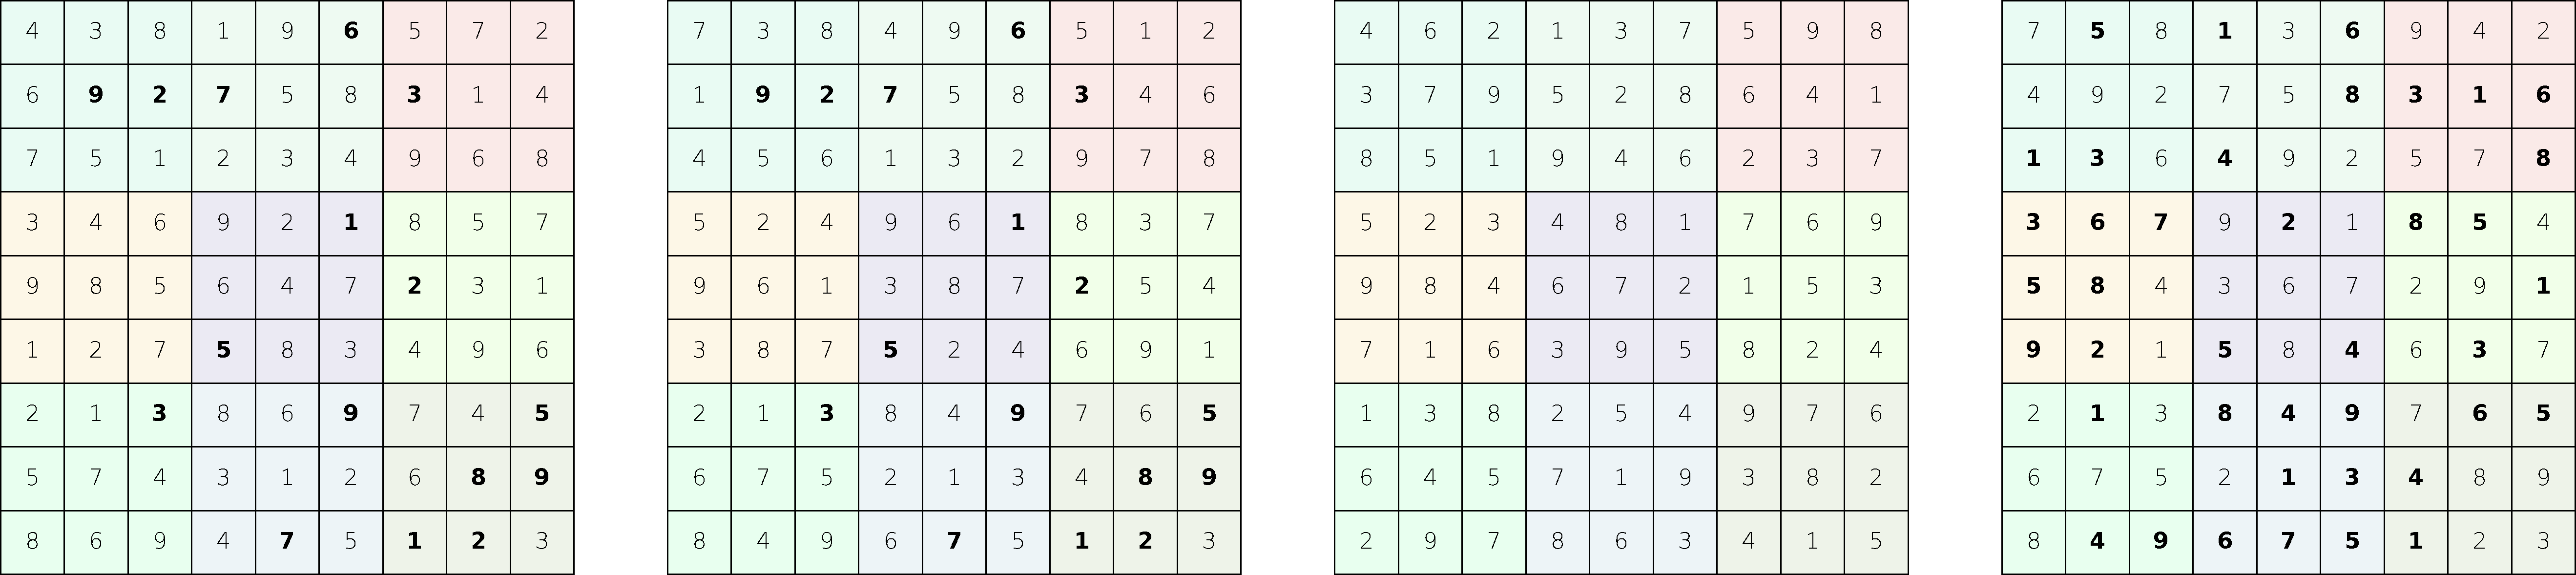
\includegraphics[width=\textwidth]{figs/thesis/sudoku_panel.pdf}
    \caption{Sudoku puzzles solved by a flexible generative model. Observed numbers (i.e. those that form part of $\rvy$) are shown in bold. The observed numbers are the same for the leftmost two Sudokus but multiple solutions exist, and we show that the generative model is able to find two different solutions. In the third Sudoku from the left, no numbers were observed. This corresponds to the task with $\gY = \{\}$. The training task distribution $u(\gY)$ covered such tasks and so this flexible generative model is capable of unconditional generation as shown. }
    \label{fig:sudoku-panel}
\end{figure}
We end this section with an intuitive example of a task where flexible conditioning is required: solving Sudoku puzzles~\citep{weilbach2023graphically}. A Sudoku is a $n^2 \times n^2$ grid of integers, each of which takes a value in $\{1,\ldots,n^2\}$. Most commonly, $n$ is set to three so the grid has size $9 \times 9$. There are three types of constraint required for a Sudoku to be valid: no value can appear more than once within the same row of the grid; no value can appear more than once within the same column; and no value can appear more than once within any of the $n^2$ $n \times n$ sub-grids that make up the grid. Sudoku puzzles are puzzles in which the player is given a Sudoku with many values missing. The player is then required to fill in the missing values. Most puzzles are constructed to have a single solution, but if the values in sufficiently few cells are given then multiple solutions can be possible. We can frame solving Sudokus as a conditional generative modelling problem if we have a data distribution $\pdata(\rvx)$ that places probability mass over all complete and valid Sudoku grids.\footnote{Fortunately this distribution is efficient to sample from. We follow the procedure from \url{https://turtletoy.net/turtle/5098380d82}.} The set of observed indices $\gY$ denotes which cells the user is given values for, and the user must infer the values for all cells not in $\gY$. The cells whose values are given as clues vary between different Sudoku puzzles, and so training a conditional generative model that can solve any given Sudoku puzzle means training a flexible generative model. 

We trained a flexible model with a very simple training task distribution that uniformly samples how many cells to observe the values of from between zero and $n^4-1$ (the number of cells minus one) and then uniformly samples this many cell indices to construct $\gY$. We process the input to the neural network by replacing elements of $\rvx_\sigma$ corresponding to observed values with those observed values. The network then performs a linear projection of each resulting value and adds a learned embedding to elements with observed values. This forms the input to a transformer-based architecture~\citep{vaswani2017attention}. We refer to \citet{weilbach2023graphically} for further details of the architecture and training procedure.

\section{Outline of the remaining chapters}
In the chapters that follow we will expand on the flexible generative modelling framework in several ways. First, in \cref{ch:fdm}, we will define a flexible diffusion model that is capable of ``marginalising out'' dimensions in the original data that we do not wish to sample or condition on. To do so we will modify \cref{eq:flexible-diffusion-target} to additionally condition on $\gX$, the indices of dimensions we wish to generate and then sample the values of only those $|\gX|$ elements. This will let us scale the flexible generative modelling framework to large and complex data in the form of long videos. In \cref{ch:tddm} we will explore how to build flexible generative models for the case where the data has varying dimensionality and $\pdata(\rvx | \rvy, \gY)$ is a trans-dimensional distribution from which different samples can have different dimensionality. In this case, conditioning on $\gY$ also implies conditioning on $\rvx$ having at least as many dimensions as suggested by the largest index in $\gY$. In \cref{ch:cigcvae} we will explore how to build a flexible generative model for the image domain based on the variational auto-encoder framework. We end by discuss our final conclusions and outlook in \cref{ch:conclusion}.

\clearpage
\chapter{Flexible diffusion modelling of long videos}
\label{ch:fdm}

We have described the flexible diffusion paradigm, but challenges remain in applying it to complex and high-dimensional data. In this chapter we will explore and tackle these challenges with a focus on the video domain, in which data is both complex and high-dimensional. More precisely, we will describe two major contributions. The first is to apply diffusion models to video generative modelling, which by itself yields significantly better photorealism than prior work. The second is a tweak to the flexible diffusion framework that enables flexible generative modelling of videos up to a thousand frames long. The models we train can be conditioned on e.g. the first frame, last frame, a series of key frames, combinations of these, or any other set of frames. As well as enabling such flexible conditioning, we show that our flexible diffusion approach improves upon standard diffusion-based approaches in terms of sample quality.

To explain why flexible diffusion can bring such benefits, we point out that, prior to the work described in this chapter, there already existed methods for modelling short photo-realistic videos (e.g. 30 frames~\citep{weissenborn2019scaling}, 48 frames~\cite{clark2019adversarial} or 64 frames~\citep{ho2022video}). There did not exist methods for generating longer videos that are both coherent and photo-realistic, which we believe is a much harder challenge. One major difficulty is scaling: photorealistic image generative models~\citep{child2020very,dhariwal2021diffusion} are already close to the memory and processing limits of modern hardware.  A long video is at very least a concatenation of many photorealistic frames, implying resource requirements, long-range coherence notwithstanding, that scale with frame count. Attempting to model such long-range coherence makes the problem harder still, especially because in general every frame can have statistical dependencies on other frames arbitrarily far back in the video. And while deep generative models based on recurrent neural networks (RNN) theoretically impose no such conditional independence assumptions, in practice they must be trained over short sequences~\cite{gruslys2016memory,saxena2021clockwork} or with truncated gradients~\citep{tallec2017unbiasing}.  Despite this, some RNN-based video generative models have demonstrated longer-range coherence, albeit without yet achieving convincing photorealistic video generation~\citep{saxena2021clockwork,babaeizadeh2021fitvid,denton2018stochastic,kim2019variational,babaeizadeh2017stochastic}.


\begin{figure}[t]
    \centering
    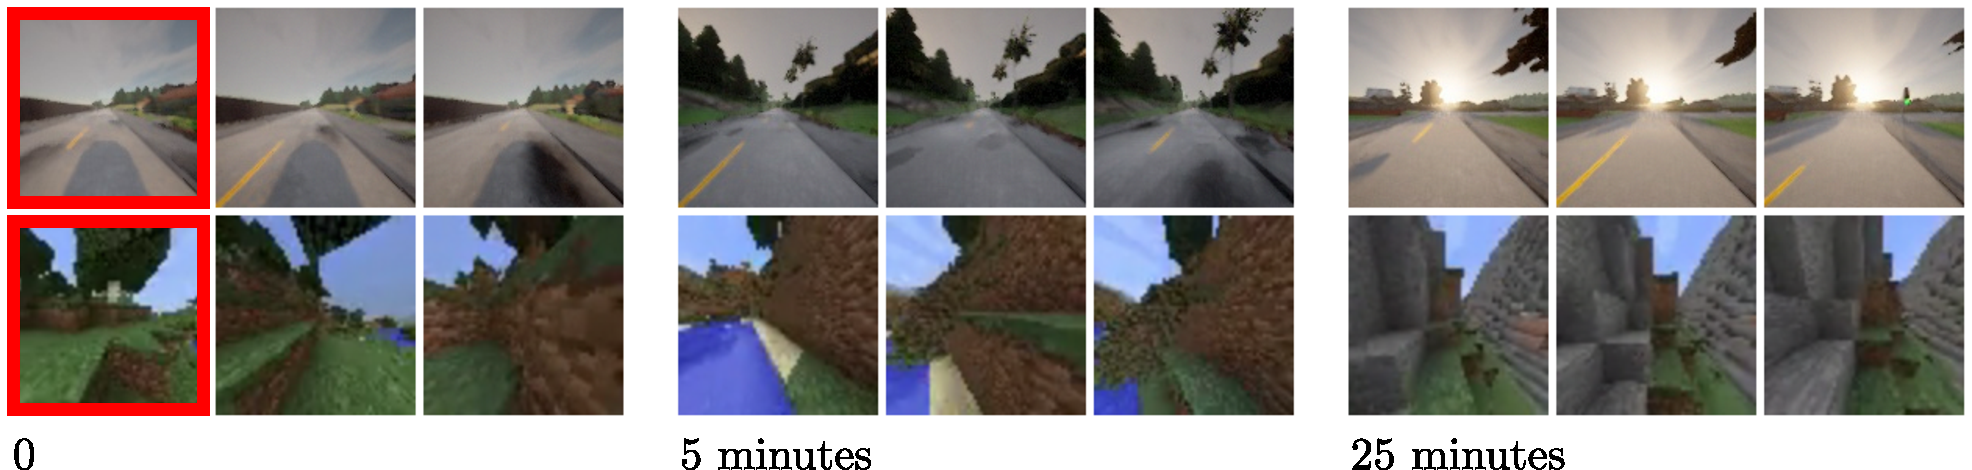
\includegraphics[width=\textwidth]{figs/fdm/fig1.pdf}
    \caption{A long video (25 minutes, or approximately 15\,000 frames) generated by FDM for each of CARLA Town01 and MineRL, conditioned on 500 and 250 prior frames respectively. We show blocks of frames from three points within each video, starting from the final observed frame on the left. Blocks are marked with the time elapsed since the last observation and frames within them are one second apart. We observe no degradation in sample quality even after $>15\,000$ frames.}
    \label{fig:fdm-1}
\end{figure}

To enable such convincing long video generation, 
we concurrently developed one of the first diffusion-based video generative models~\cite{ho2022video,yang2022diffusion,voleti2022mcvd}. While we see that straightforwardly applying DMs with a suitable architecture can yield improved photorealism versus previous methods, doing so does not automatically solve the problems of modelling long-range dependencies. DMs can still only model a limited number of frames at a time, and so techniques like autoregressive roll-outs are needed to extend them to long videos. Unfortunately, fixed-lag autoregressive models impose unrealistic conditional independence assumptions (the next frame being independent of frames further back in time than the autoregressive lag is problematic for generating videos with long-range coherence).  

In addition to imposing these unrealistic conditional independence assumptions, autoregressive models make flexible generation difficult. They are typically designed to enable unconditional generation, and their design also makes conditioning on the first frame or set of frames simple. Other forms of conditioning, however, become difficult, in particular conditioning on frames towards the end of the video.

In this work we embrace the fact that finite architectures will always impose conditional independence assumptions and prevent us from conditioning on all that we might desire. The question we ask is: given an explicit limit $K$ on the number of video frames we can jointly model, how can we best allocate these frames to generate a video of length $N > K$? In the unconditional case, one option is to use the previously-described autoregressive model but, if $K=N/4$, we could instead follow \citet{ho2022video} by training two models: one which first samples every 4th frame in the video, and another which (in multiple stages) infills the remaining frames conditioned on those. The latter option will enable new capabilities, like conditioning on frames further from the start of the video than the autoregressive model is able to condition on. It will also be able to capture dependencies across a larger time horizon. A downside is that is will not enable conditioning on both of the first two frames, as a purely autoregressive approach would.

The diffusion model which we propose in this chapter can sample any subset of video frames conditioned on observed values of any other subset of video frames, as long as the total size of these subsets is small enough to satisfy memory constraints. It is therefore compatible with purely autoregressive sampling, sampling in two stages at two different temporal resolutions, or any other order in which to samples frames. This enables enable efficient exploration of the space of such sampling schemes and simple adaptation to different conditioning tasks or to different video lengths. We will from now on refer to the flexible diffusion model presented as FDM.

\section{Sampling long videos}


\begin{algorithm}[t]
    \centering
    \caption{Sample a video $\rvv$ given a sampling scheme $[(\mathcal{X}_s,\mathcal{Y}_s)]_{s=1}^S$. For unconditional generation, the input $\rvv$ can be a tensor of zeros. For conditional generation, the observed input frames should contain their observed values.}
    \label{alg:sampling}
    \footnotesize
    \begin{algorithmic}[1]
    \Procedure{SampleVideo}{$\rvv$; $\theta$}
        \For{$s \gets 1,\ldots,S$}
            \State $\rvy \gets \rvv [\mathcal{Y}_s]$ \Comment{Gather frames indexed by $\mathcal{Y}_s$.}
            \State $\rvx \sim  \texttt{DM}(\cdot; \rvy, \mathcal{X}_s, \mathcal{Y}_s, \theta)$  \Comment{Sample $\rvx$ from the conditional DM.}
            \State $\rvv [\mathcal{X}_s] \gets \rvx$ \Comment{Modify frames indexed by $\mathcal{X}_s$ with their sampled values.}
        \EndFor
    \EndProcedure
    \State \Return {$\rvv$}
    \end{algorithmic}
\end{algorithm}


\begin{figure*}[t!]
    \centering
    \begin{subfigure}[t]{0.24\textwidth}
        \centering
        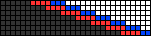
\includegraphics[width=\textwidth]{figs/fdm/unconditional-inference-modes/sample_vis_autoreg_T=30_sampling_3_out_of_7_red_blue_flipped.png}
        \caption{\footnotesize Autoregressive.} \label{fig:autoreg-vis}
    \end{subfigure}
    \begin{subfigure}[t]{0.24\textwidth}
        \centering
        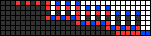
\includegraphics[width=\textwidth]{figs/fdm/unconditional-inference-modes/sample_vis_baby-cond-ho-et-al-for-vis_T=30_sampling_3_out_of_7_red_blue_flipped.png}
        \caption{\footnotesize Two temporal res.} \label{fig:google-vis}
    \end{subfigure}
    \begin{subfigure}[t]{0.24\textwidth}
        \centering
        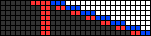
\includegraphics[width=\textwidth]{figs/fdm/unconditional-inference-modes/sample_vis_mixed-autoreg-independent_T=30_sampling_3_out_of_7_red_blue_flipped.png}
        \caption{\footnotesize Long-range (ours).} \label{fig:mixed-vis}
    \end{subfigure}
    \begin{subfigure}[t]{0.24\textwidth}
        \centering
        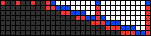
\includegraphics[width=\textwidth]{figs/fdm/unconditional-inference-modes/sample_vis_hierarchy-2_T=30_sampling_3_out_of_7_red_blue_flipped.png}
        \caption{\footnotesize Hierarchy-2 (ours).} \label{fig:hierarchy-vis}
    \end{subfigure}%
    \caption{Sampling schemes that could be used to complete a video of length $N=30$ conditioned on the first 10 frames, with access to at most $K=7$ frames at a time. Each stage $s$ of the sampling procedure is represented by one row in the figure, going from top to bottom. Within each subfigure, one column represents one frame of the video, from frame one on the left to frame 30 on the right. At each stage, the values of frames marked in blue are sampled conditioned on the (observed or previously sampled) values of frames marked in red; frames marked in grey are ignored; and frames marked in white are yet to be sampled. For every sampling scheme, all video frames have been sampled after the final row.
    }
\end{figure*}

Our goal in this paper is to sample coherent photo-realistic videos $\rvv$ with thousands of frames (see \cref{fig:fdm-1}). 
%
To sample an arbitrarily long video with a generative model that can sample or condition on only a small number of frames at once, we must use a sequential procedure. The simplest example of this is an autoregressive scheme, an example of which is shown in \cref{fig:autoreg-vis} for a video completion task. 
%
In this example it takes seven stages to sample a complete video, in that we must run the generative model's sampling procedure seven times. 
%
At each stage three frames are sampled conditioned on the immediately preceding four frames. This scheme is appealing for its simplicity but imposes a strong assumption that, given the set of four frames that are conditioned on at a particular stage, all frames that come afterwards are conditionally independent of all frames that came before. This restriction can be partially ameliorated with the sampling scheme shown in \cref{fig:google-vis} where, in the first three stages, every second frame is sampled and then, in the remaining four stages, the remaining frames are infilled. One way to implement this would be to train two different models operating at the two different temporal resolutions. 
%
In the language of \citet{ho2022video}, who use a similar approach, sampling would be carried out in the first three stages by a ``frameskip-2'' model and, in the remaining stages, by a ``frameskip-1'' model. Both this approach and the autoregressive approach are examples of what we call \textit{sampling schemes}.
%
More generally, we characterise a sampling scheme as a sequence of tuples $[(\mathcal{X}_s, \mathcal{Y}_s)]_{s=1}^S$, each containing a vector $\mathcal{X}_s$ of indices of frames to sample and a vector $\mathcal{Y}_s$ of indices of frames to condition on for stages $s = 1,\ldots,S$. 

\Cref{alg:sampling} lays out how such a sampling scheme is used to sample a video. If the underlying generative model is trained specifically to model sequences of consecutive frames, or sequences of regularly-spaced frames, then the design space for sampling schemes compatible with these models is severely constrained. In this paper we take a  different approach.  We design and train a generative model to sample any arbitrarily-chosen subset of video frames conditioned on any other subset and train it using an entirely novel distribution of such tasks. In short, our model is trained to generate frames for any choice of $\mathcal{X}$ and $\mathcal{Y}$. The only constraint we impose on our sampling schemes is therefore a computational consideration that $|\mathcal{X}_s| + |\mathcal{Y}_s| \leq K$ for all $s$ but, to generate meaningful videos, any valid sampling scheme must also satisfy two more constraints: (1) all frames are sampled at at least one stage and (2) frames are never conditioned upon before they are sampled.

Such a generative model allows us to explore and use sampling schemes like those in \cref{fig:mixed-vis} and \cref{fig:hierarchy-vis}.  We find in our experiments that the best video sampling scheme is dataset dependent. Accordingly, later in this chapter we will present methodology to optimise such sampling schemes in a dataset dependent way, leading to improved video quality as measured by the Fréchet Video Distance~\cite{unterthiner2018towards} among other metrics. We now discuss FDM's architecture, the specific task distribution  used to train it, and the choice and optimisation of sampling schemes in \cref{sec:fdm-architecture}.

\begin{figure*}[t]
    \centering
    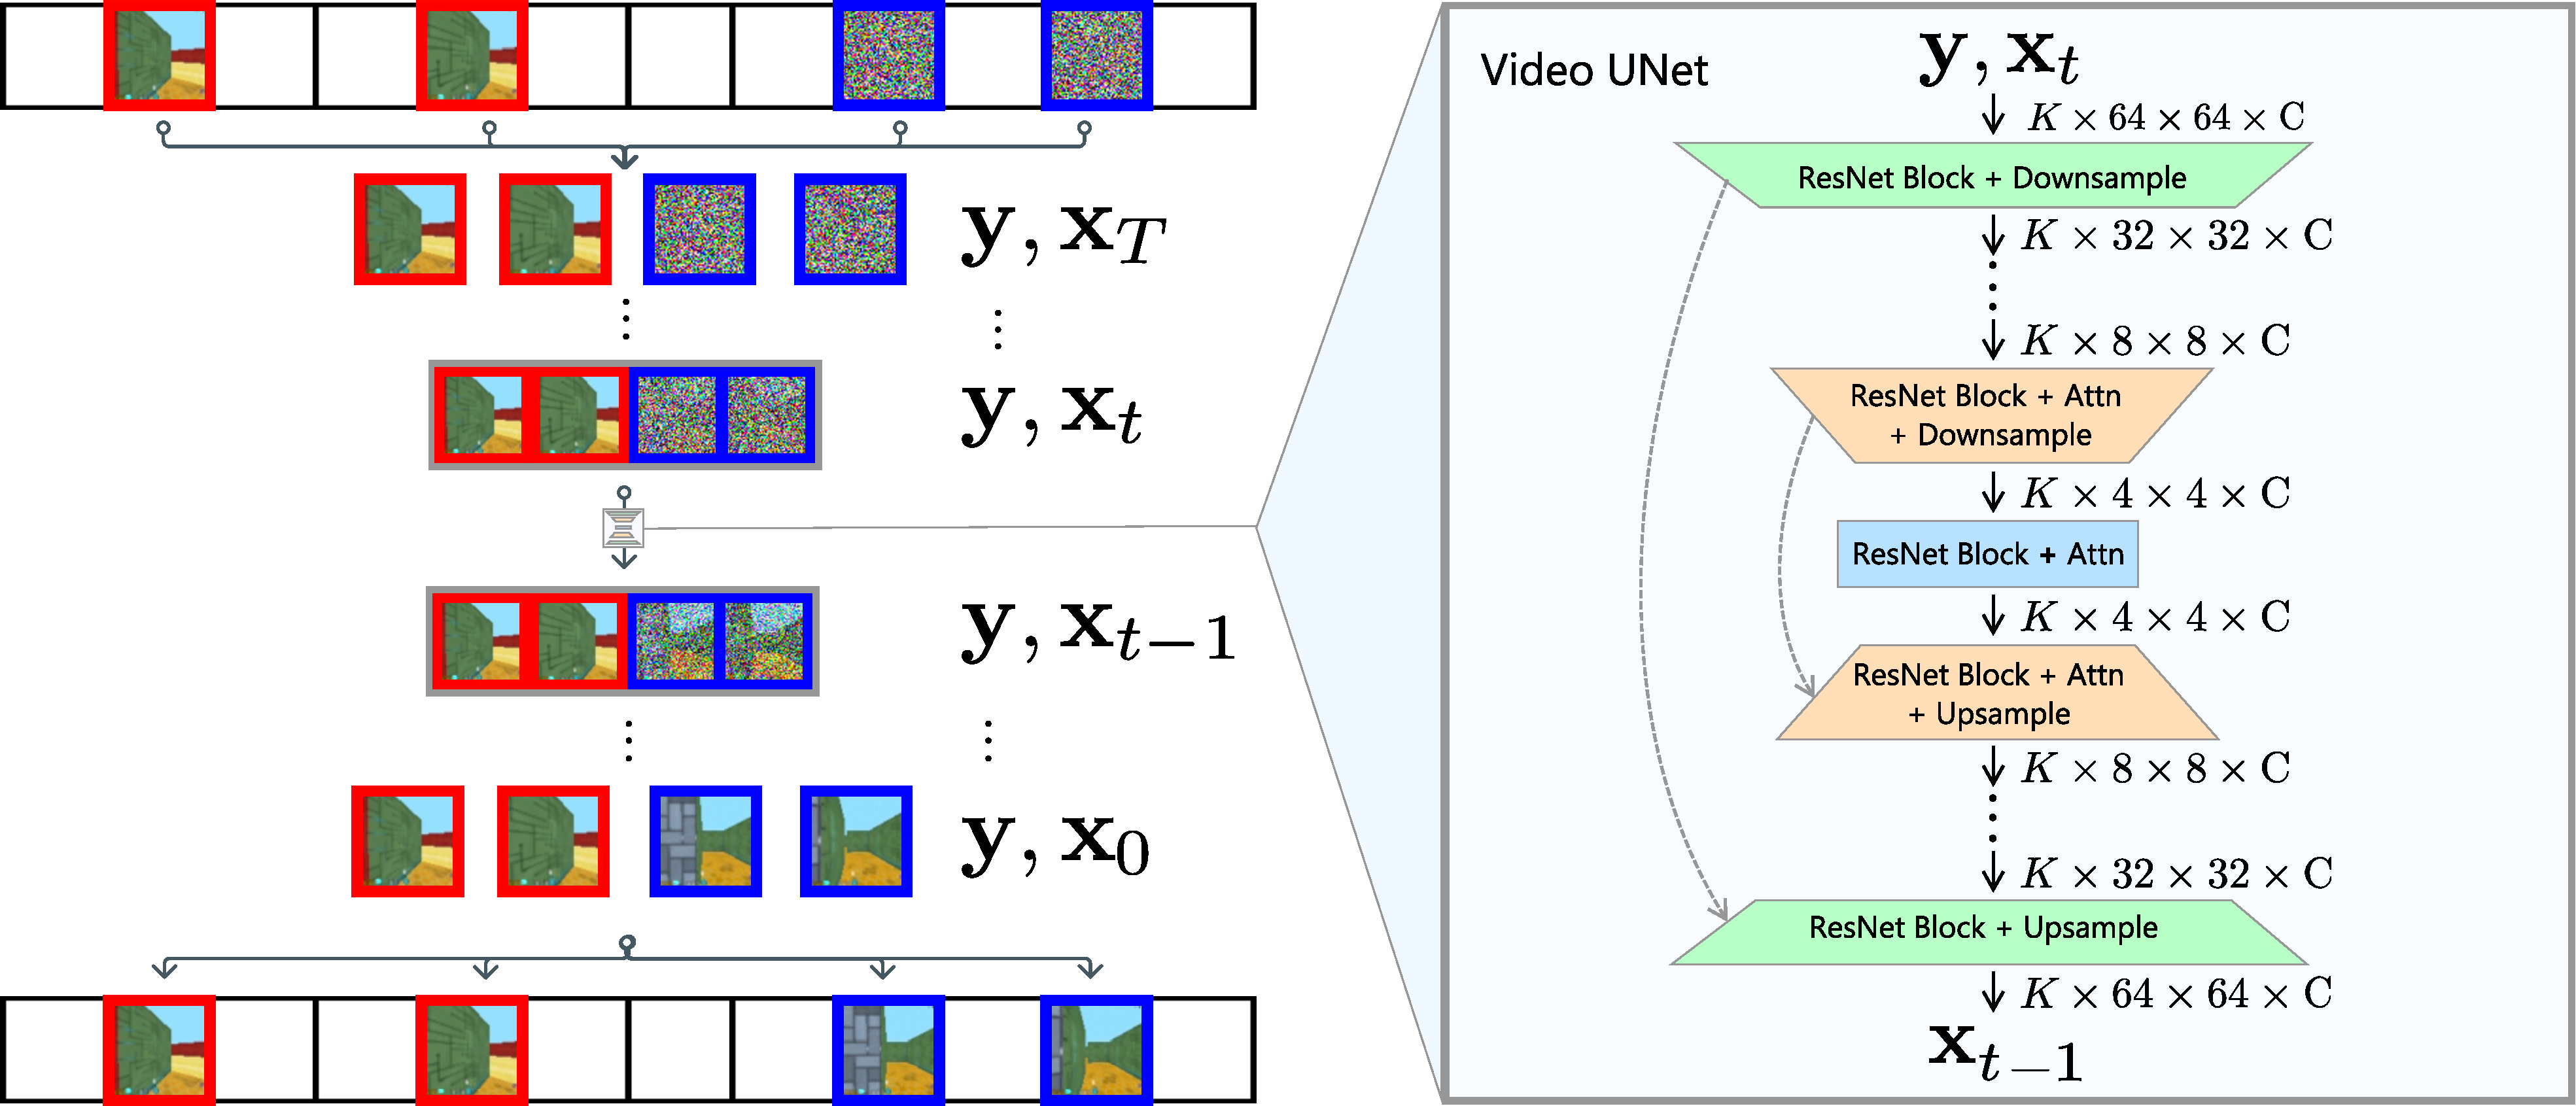
\includegraphics[width=0.88\textwidth]{figs/fdm/video-architecture-v8.pdf}
    \caption{A visualisation of our flexible video diffusion model and its neural architecture. \textbf{Left:} Our DM iteratively transforms Gaussian noise $\rvx_T$ to video frames $\rvx_0$ (shown with blue borders), conditioning on observed frames $\rvy$ (red borders) at every step. \textbf{Right:} The U-net architecture used within each DM step. It computes $\epsilon_\theta(\rvx_t, \rvy, t)$, which is used to transition the state from $\rvx_t$ to $\rvx_{t-1}$ as described in \cref{ch:diffusion}.
    }
    \label{fig:architecture}
\end{figure*}

\section{Training procedure and architecture}\label{sec:fdm-method}

\paragraph{Flexible diffusion objective with marginalisation}
We now present our modification of the flexible diffusion training objective that enables us to vary not just which frames are conditioned on, but also which are generated as opposed to being ``marginalised out''. In \cref{ch:flexible-diffusion} we varied the indices of values to condition on, $\gY$, between training examples, and trained the model to sample all other values. In this chapter we only want the model to sample a subset of the other values so we will introduce, $\gX$, the indices of the values to generate. We will use $\gX$ as an input to the model and vary it between training examples. We rename the original data points $\rvv$ to distinguish them from the objects that the model is trained to generate, $\rvx := \rvv[\gX]$ (i.e. the components of $\rvv$ at indices in $\gX$). We then modify the flexible diffusion objective from \cref{eq:flexible-diffusion-loss} to give the flexible diffusion modelling with marginalisation objective:
\begin{align} \label{eq:fdm-loss}
    \mathcal{L}_\text{FDMM}(\theta) &= 
    % \int_{\sigma_\text{min}}^{\sigma_\text{max}}  
    \EX_{u(\sigma) u(\rvx, \rvx_\sigma, \rvy, \gX, \gY)} \frac{\lambda^\rvx(\sigma)}{u(\sigma)} \left[ 
    || \predx_\theta(\rvx_\sigma, \rvy, \sigma, \gX, \gY) - \rvx ||_2^2 \right]
\end{align}
with $u(\rvx, \rvx_\sigma, \rvy, \gX, \gY) = \int u(\gX, \gY)\pdata(\rvv)\delta(\rvx,\rvy|\rvv,\gX,\gY)q(\rvx_\sigma|\rvx) \mathrm{d}\rvv$. We will call $u(\gX, \gY)$ the training task distribution and give a precise specification in the next paragraph ; $\pdata(\rvv)$ is our distribution of long training videos ; $\delta(\rvx,\rvy|\rvv,\gX,\gY)$ is a Dirac distribution which returns $\rvx = \rvv[\gX]$ and $\rvy = \rvv[\gY]$ ; and $q(\rvx_\sigma | \rvx)$ is the standard diffusion ``noising'' distribution as defined in \cref{ch:diffusion}. Recall that, in the standard flexible diffusion setting, the dimensionality of $\rvy$ could vary but that of $\rvx$ was fixed. In the new setting, the dimensionalities of both $\rvx$ and $\rvy$ can vary.

\paragraph{Diffusion process details}
We use variance-preserving diffusion process as described in \cref{sec:more-general-diffusion-processes}, use a discrete-time formulation as described in \cref{sec:diffusion-discrete-time} with 1000 discrete timesteps, and sample with a DDPM-style sampler. See \cref{app:fdm} for full detail.

\paragraph{Training task distribution}
Different choices of latent and observed indices $\mathcal{X}$ and $\mathcal{Y}$ can be regarded as defining different conditional generation tasks. In this sense, we aim to learn a model which can work well on any task (i.e. any choice of $\mathcal{X}$ and $\mathcal{Y}$) and so we randomly sample these vectors of indices during training. We do so with the distribution $u(\latindices,\obsindices)$ described in \cref{fig:training-distribution}. It provides a broad distribution covering many plausible test-time use cases while still providing a better learning signal than a uniform distribution (see ablation in \cref{sec:fdm-experiments} and more details in \cref{ap:fdm-training-task-distribution-ablation}). To cope with constrained computational resources, the distribution is designed such that $|\mathcal{X}|+|\mathcal{Y}|$ is upper-bounded by some pre-specified $K$. Sampling from $q(\rvx, \rvy)$ to compute the our objective (\cref{eq:fdm-loss}) is then accomplished by randomly selecting both a full training video $\rvv$ from the dataset and indices $\mathcal{X},\mathcal{Y}\sim u(\cdot,\cdot)$. We then extract the specified frames $\rvx = \rvv[\latindices]$ and $\rvy = \rvv[\obsindices]$ (where we use $\rvv[\latindices]$ to denote the concatenation of all frames in $\rvv$ with indices in $\latindices$ and and $\rvv[\obsindices]$ similarly).

\begin{figure}
\begin{minipage}[t]{0.33\textwidth}
\begin{figure}[H]
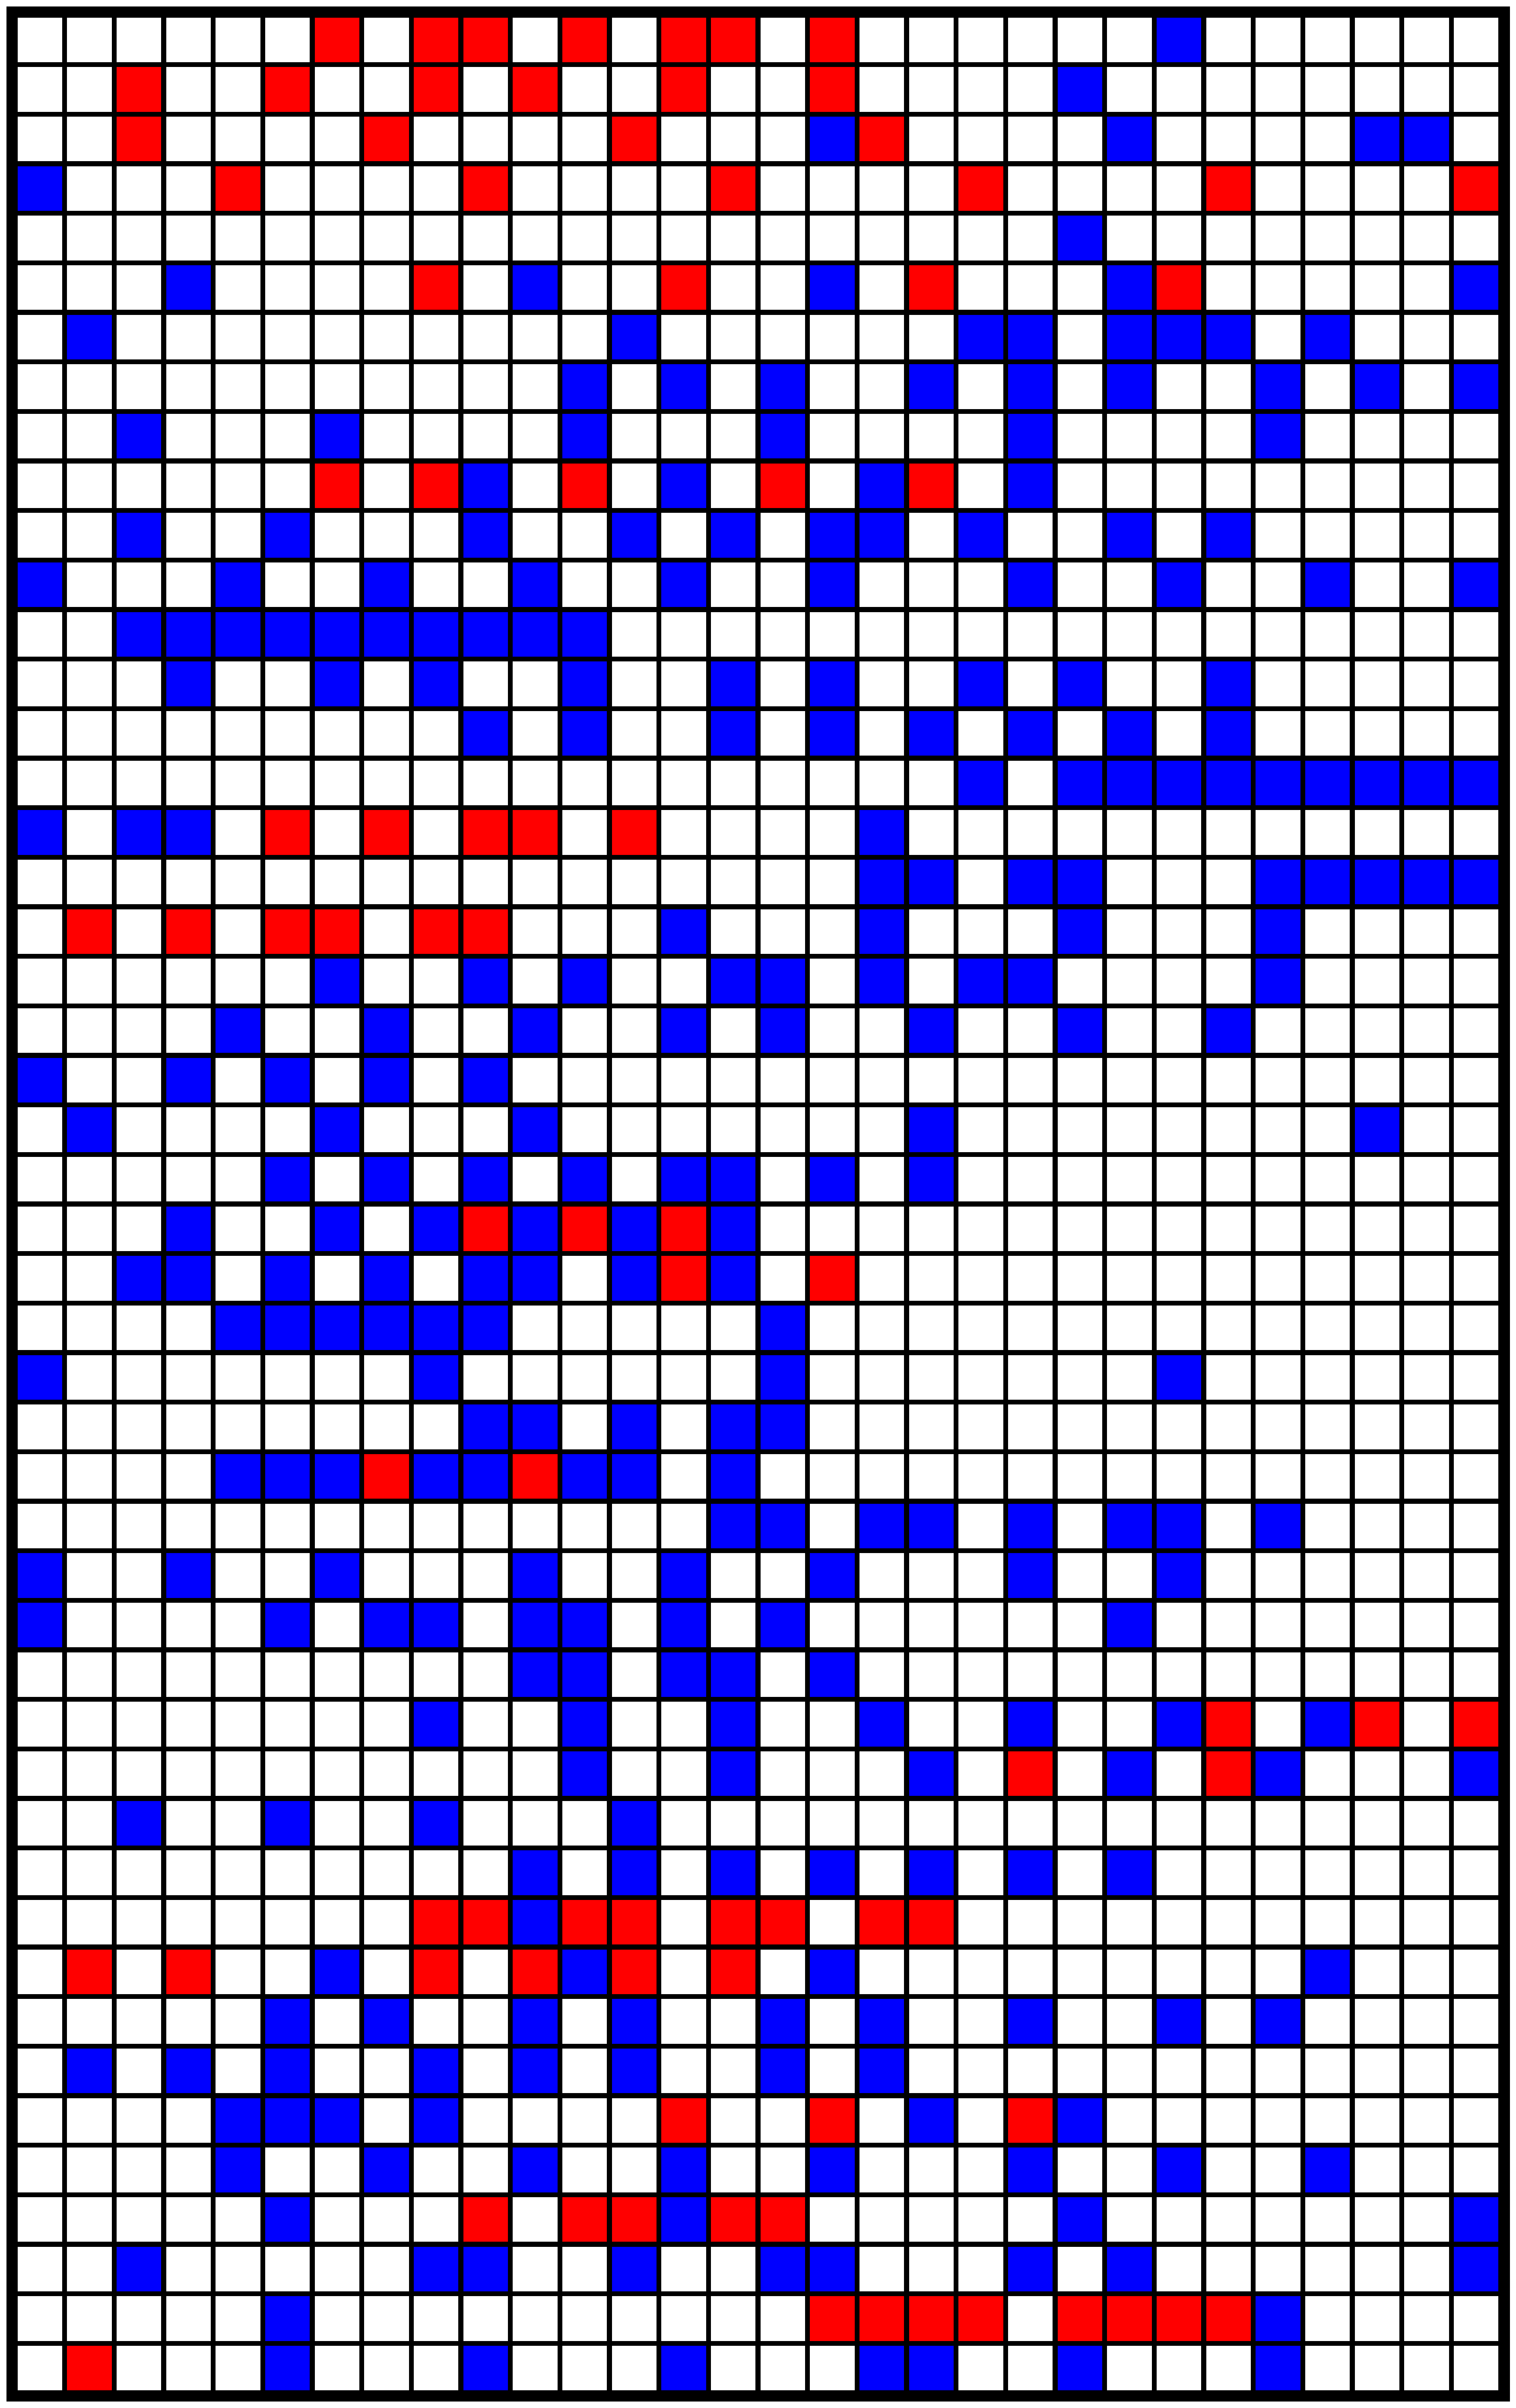
\includegraphics[width=\textwidth]{figs/fdm/training-2.pdf}
\end{figure}
\end{minipage}
\hfill
\begin{minipage}[t]{0.65\textwidth}
\begin{algorithm}[H]
    \caption{Sampling training tasks $\latindices,\obsindices\sim u(\cdot)$ given $N,K$.}\label{alg:mask-distribution}
    \label{alg:training-distribution}
    \footnotesize
    \begin{algorithmic}[1]
      \State $\latindices := \{\}$; $\obsindices := \{\}$
      \While{True}
        \State $n_\text{group} \sim \text{UniformDiscrete}(1, K)$ %\Comment{Sample number of frames in the group}
        \State $s_\text{group} \sim \text{LogUniform}(1, (N-1)/n_\text{group})$ %\Comment{Sample spacing between frames}
        \State $x_\text{group} \sim \text{Uniform}(0, N-(n_\text{group}-1)\cdot s_\text{group})$ %\Comment{Sample position of first frame in the group}
        \State $o_\text{group} \sim \text{Bernoulli}(0.5)$
        \State $\mathcal{G} := \{\lfloor x_\text{group} + s_\text{group} \cdot i \rfloor | i \in \{0,\ldots,n_\text{group}-1\} \} \setminus \latindices \setminus \obsindices$ \label{line:make-G}
        \If{$|\latindices| + |\obsindices| + |\mathcal{G}| > K$}
            \State \Return {$\texttt{set2vector}(\latindices),\texttt{set2vector}(\obsindices)$}
        \ElsIf{$|\latindices| = 0$ \textbf{or} $o_\text{group} = 0$} \label{line:obs-or-lat}
            \State $\latindices := \latindices \cup \mathcal{G}$
        \Else
            \State $\obsindices := \obsindices \cup \mathcal{G}$
        \EndIf
    \EndWhile
    \end{algorithmic}
\end{algorithm}
\end{minipage}
\caption{Samples from our distribution over training tasks, $u(\mathcal{X},\mathcal{Y})$, along with psuedocode for drawing them. \textbf{Left:} Samples with video length $N=30$ and limit $K=10$ on the number of sampled indices. Each row shows one sample and columns map to frames, with frame 1 on the left and frame $N$ on the right. Blue and red denote latent and observed frames respectively. All other frames are ignored and shown as white. \textbf{Right:} Pseudocode for drawing these samples. The while loop iterates over a series of regularly-spaced groups of latent variables. Each group is parameterised by: the number of indices in it, $n_\text{group}$; the spacing between indices in it, $s_\text{group}$; the position of the first frame in it, $x_\text{group}$, and an indicator variable for whether this group is observed, $o_\text{group}$ (which is ignored on line~\ref{line:obs-or-lat} if $\mathcal{X}$ is empty to ensure that the returned value of $\mathcal{X}$ is never empty). These quantities are sampled in a continuous space and then discretised to make a set of integer coordinates on line~\ref{line:make-G}. The process repeats until a group is sampled which, if added to $\latindices$ or $\obsindices$, will cause the number of frames to exceed $K$. That group is then discarded and $\mathcal{X}$ and $\mathcal{Y}$ are returned as vectors. The FDM's training objective forces it to work well for any $(\mathcal{X},\mathcal{Y})$ pair from this broad distribution.
}
\label{fig:training-distribution}
\end{figure}

\paragraph{Architecture}
\label{sec:fdm-architecture}
Image diffusion models~\citep{ho2020denoising,nichol2021improved} typically use a U-net architecture~\cite{ronneberger2015u}. Its distinguishing feature is a series of spatial downsampling layers followed by a series of spatial upsampling layers, and these are interspersed with convolutional ResNet blocks~\cite{he2015deep} and spatial attention layers. Since we require an architecture which operates on 4-D video tensors rather than 3-D image tensors we add an extra \textit{frame} dimension to its input, output and hidden state, resulting in the architecture shown on the right of \cref{fig:architecture}. We create the input to this architecture as a concatenation $\rvx_t \oplus \rvy$, adding an extra input channel which is all ones for observed frames and all zeros for latent frames. For RGB video, the input shape is therefore $(K, \textit{image height}, \textit{image width}, 4)$. Since the output should have the same shape as $\rvx_t$ we only return outputs corresponding to the latent frames, giving output shape  $(|\latindices|, \textit{image height}, \textit{image width}, 3)$. We run all layers from the original model (including convolution, resizing, group normalisation, and spatial attention) independently for each of the $K$ frames.
To allow communication between the frames, we add a temporal attention layer after each spatial attention layer, described in more detail in the appendix. 
%
The spatial attention layer allows each spatial location to attend to all other spatial locations \textit{within} the same frame, while the temporal attention layer allows each spatial location to attend to the same spatial location across all \textit{other} frames.
%
This combination of a temporal attention layer with a spatial attention layer is sometimes referred to as \textit{factorised attention}~\citep{tashiro2021csdi,ho2022video}. We found that, when using this architecture in conjunction with our meta-learning approach, performance could be improved by using a novel form of relative position encoding~\cite{shaw2018self,wu2021rethinking}. We describe this in greater detail in \cref{app:fdm-rpe}.


\paragraph{Training batch padding}
Although the size $|\latindices\oplus\obsindices|$ of index vectors sampled from our training distribution is bounded above by $K$, it can vary. To fit examples with various sizes of index vectors into the same batch, one option would be to pad them all to length $K$ with zeros and use masks so that the zeros cannot affect the loss. This, however, would waste computation on processing tensors of zeros.
%
We instead use this computation to obtain a lower-variance loss estimate by processing additional data with ``training batch padding''.
%
This means that, for training examples where $|\latindices\oplus\obsindices| < K$, we concatenate frames uniformly sampled from a second video to increase the length along the frame-dimension to $K$. Masks are applied to the temporal attention mechanisms so that frames from different videos cannot attend to eachother and the output for each is the same as that achieved by processing the videos in different batches.

\paragraph{Sampling schemes}
Before describing the sampling schemes we experiment with, we emphasise that the relative performance of each is dataset-dependent and there is no single best choice. A central benefit of FDM is that it can be used at test-time with different sampling schemes without retraining. Our simplest sampling scheme, \textbf{Autoreg}, samples ten consecutive frames at each stage conditioned on the previous ten frames. \textbf{Long-range} is similar to Autoreg but conditions on only the five most recent frames as well as five of the original 36 observed frames. \textbf{Hierarchy-2} uses a multi-level sampling procedure. In the first level, ten evenly spaced frames spanning the non-observed portion of the video are sampled (conditioned on ten observed frames). In the second level, groups of consecutive frames are sampled conditioned on the closest past and future frames until all frames have been sampled. \textbf{Hierarchy-3} adds an intermediate stage where several groups of variables with an intermediate spacing between them are sampled. We include Adaptive Hierarchy-2, abbreviated \textbf{Ad. hierarchy-2}, as a demonstration of a sampling scheme only possible with a model like FDM. It samples the same frames at each stage as Hierarchy-2 but selects which frames to condition on adaptively at test-time with a heuristic aimed at collecting the maximally diverse set of frames, as measured by the pairwise LPIPS distance~\cite{zhang2018unreasonable} between them.

\paragraph{Optimising sampling schemes}
An appealing alternative to the heuristic sampling schemes described in the previous paragraph would be to find a sampling scheme that is, in some sense, optimal for a given model and video generation/completion task. While it is unclear how to tractably choose which frames should be sampled at each stage, we suggest that the frames to condition on at each stage can be chosen by greedily optimising the diffusion model loss which, as detailed in \cref{ch:diffusion}, is closely related to the data log-likelihood. Given a fixed sequence of frames to sample at each stage $[\latindices_s]_{s=1}^S$ we select $\obsindices_s$ for each $s$ to minimise the variation of \cref{eq:fdm-loss},
\begin{align}
    % \int_{\sigma_\text{min}}^{\sigma_\text{max}} 
    \EX_{u(\sigma)u(\rvx, \rvx_\sigma, \rvy|\gX_s, \gY_s)} \left[
    \frac{\lambda^\rvx(\sigma)}{u(\sigma)}
    || \predx_\theta(\rvx_\sigma, \rvy, \sigma, \gX_s, \gY_s) - \rvx ||_2^2 \right].
\end{align}
This is estimated using a set of 100 training videos and by iterating over 10 evenly-spaced values of $t$ (which reduced variance relative to random sampling of $t$). See the appendix for further details. We create two optimised sampling schemes: one with the same latent indices as Autoreg, and one with the same latent indices as Hierarchy-2. We call the corresponding optimised schemes \textbf{Opt. autoreg} and \textbf{Opt. hierarchy-2}.


\begin{figure}
    \centering
    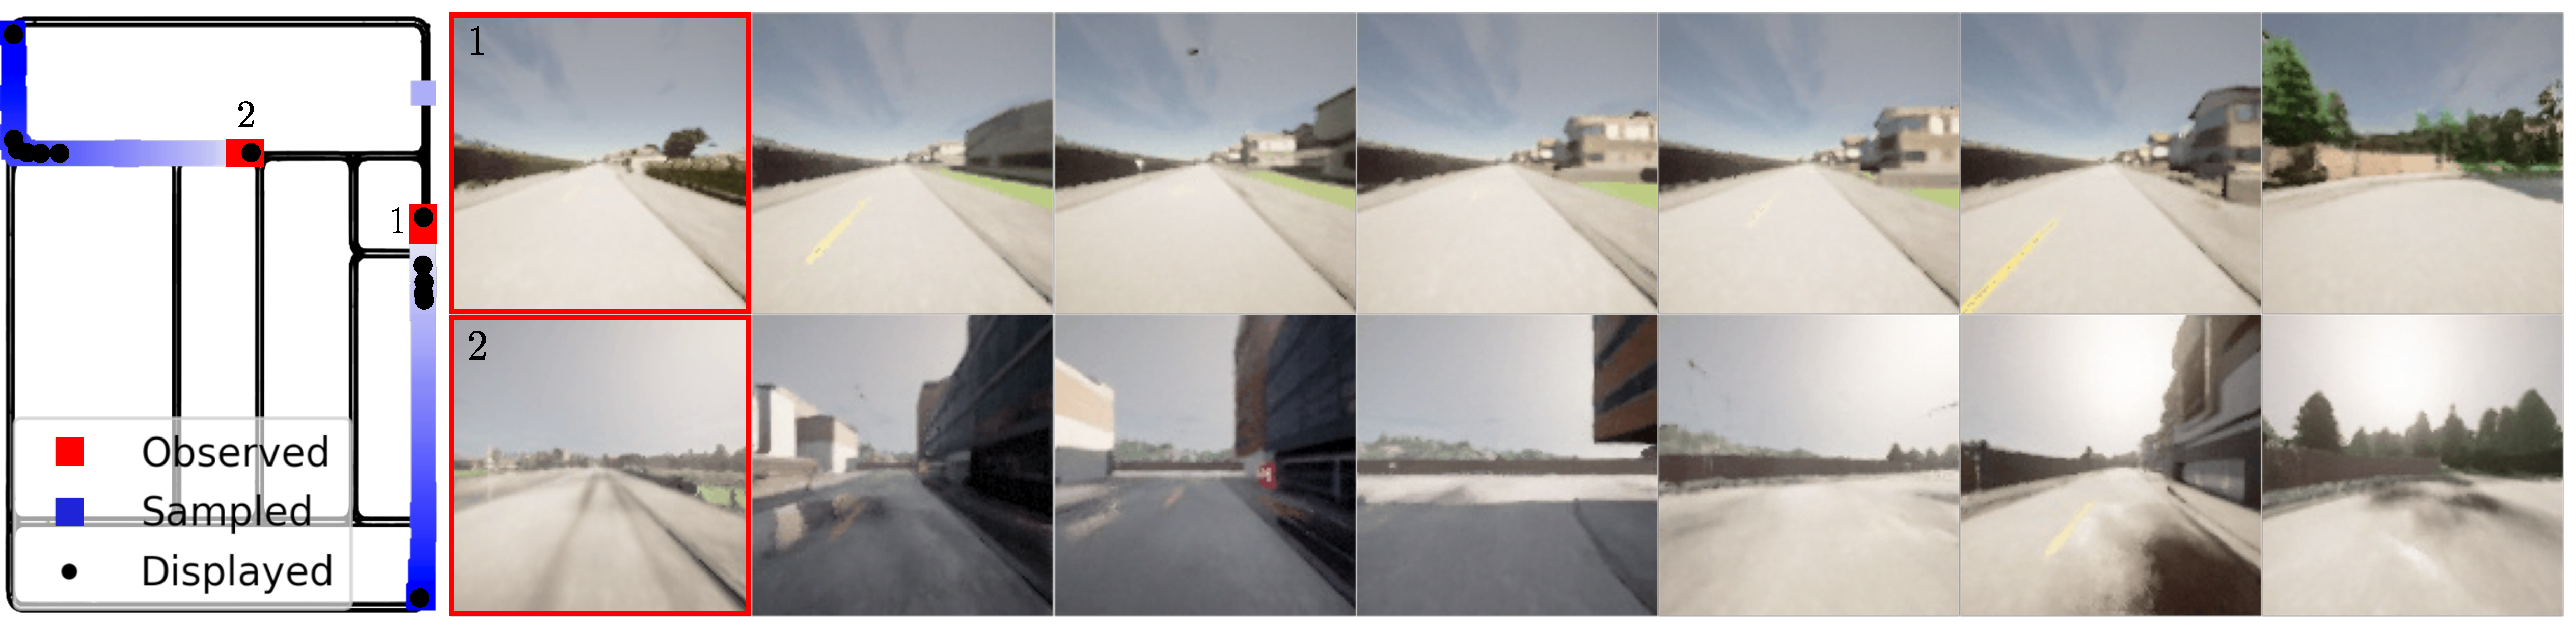
\includegraphics[width=1\textwidth]{figs/fdm/carla_map_7panel}
    \caption{Visualisation of video completions on the CARLA Town01 dataset. \textbf{Left:} Map of the town featured in the CARLA Town01 dataset. We visualise two video completions by FDM by showing coordinates output by our regressor (as discussed in \cref{sec:fdm-carla}) for each frame. Those corresponding to the initial 36 observed frames are shown in red and those for the 964 sampled frames are shown in blue. \textbf{Right:} For each completion, we show one of the initially observed frames followed by four of the sampled frames (at positions chosen to show the progression with respect to visible landmarks and marked by black dots on the map). The town's landmarks are usually sampled with high-fidelity, which is key to allowing the regressor  to produce a coherent trajectory on the left. However there are sometimes failures: a blue square near the top-right of the map shows where the video model ``jumped'' to a wrong location for a single frame.}
    \label{fig:carla}
\end{figure}


\section{CARLA Town01 dataset}
\label{sec:fdm-carla}
In this section we propose a new video modelling dataset and benchmark which provides an interpretable measure of video completion quality. The dataset consists of videos of a car driving with a first-person view, produced using the CARLA autonomous driving simulator~\cite{dosovitskiy2017carla}. All 408 training and 100 test videos (of length 1000 frames and resolution $128\times128$) are produced within a single small town, CARLA's Town01. As such, when a sufficiently expressive video model is trained on this dataset it memorises the layout of the town and videos sampled from the model will be recognisable as corresponding to routes travelled within the town. We train a regression model in the form of a neural network which maps with high accuracy from any single rendered frame to $(x,y)$ coordinates representing the car's position. Doing so allows us to plot the routes corresponding to sampled videos (see left of \cref{fig:carla}) and compute semantically-meaningful yet quantitative measures of the validity of these routes. Specifically, we compute histograms of speeds, where each speed is estimated by measuring the distance between the regressed locations for frames spaced ten apart (1 second at the dataset's frame rate). Sampled videos occasionally ``jump'' between disparate locations in the town, resulting in unrealistically large estimated speeds. To measure the frequency of these events for each method, we compute the percentage of our point-speed estimates that exceed a threshold of $10$m/s (the dataset was generated with a maximum simulated speed of $3$m/s). We report this metric as the outlier percentage (OP). After filtering out these outliers, we compute the Wasserstein distance (WD) between the resulting empirical distribution and that of the original dataset, giving a measure of how well the speeds in generated videos match the speeds in dataset videos. We have released the CARLA Town01 dataset and trained regression model along with the rest of our code to allow future comparisons.\footnote{\url{https://github.com/plai-group/flexible-video-diffusion-modeling}}

\section{Experiments} \label{sec:fdm-experiments}

We perform our main comparisons on the video completion task. For this task, in keeping with \citet{saxena2021clockwork}, we condition on the first 36 frames of each video and sample the remainder. We present results on three datasets: GQN-Mazes~\citep{eslami2018neural}, in which videos are 300 frames long; MineRL Navigate~\citep{guss2019minerl,saxena2021clockwork} (which we will from now on refer to as simply MineRL), in which videos are 500 frames long; and the CARLA Town01 dataset we release, for which videos are 1000 frames long. We train FDM in all cases with the maximum number of represented frames $K=20$. We host non-cherry-picked video samples (both conditional and unconditional) from FDM and baselines online\footnote{\url{https://www.cs.ubc.ca/~wsgh/fdm}}.


\begin{table*}
  \scriptsize
  \caption{Evaluation of video completions by our method (FDM) with various sampling schemes along with several baselines from the literature. Error bars denote the standard error computed with 5 random seeds. Higher is better for the accuracy metric~\cite{saxena2021clockwork} and lower is better for all other metrics shown.}
  \label{tab:fdm-results-completion}
  \centering
  \begin{tabular}{llllllll}
    \toprule
    \multicolumn{1}{r}{} & & \multicolumn{2}{c}{GQN-Mazes}  & \multicolumn{1}{c}{MineRL}  & \multicolumn{3}{c}{CARLA Town01} \\
    \cmidrule(r){3-4} \cmidrule(r){5-5} \cmidrule(r){6-8}
    Model &  Sampling scheme        & FVD      & Accuracy  & FVD     &  FVD     & WD  & OP \\
    \midrule
    \multirow{1}{*}{CWVAE~\citep{saxena2021clockwork}}
    & CWVAE  & $837 \pm 8$      & $82.6 \pm 0.5$  & $1573 \pm 5$                 & $1161$          & $0.666$   & $44.4$        \\
    \midrule
    \multirow{1}{*}{TATS~\citep{ge2022long}}
    & TATS   & $163 \pm 2.6$  &  $77.0 \pm 0.8$  & $807 \pm 14$          & $329$          & $1.648$          & $42.4$ \\
    \midrule
    \multirow{1}{*}{VDM~\citep{ho2022video}}
    & VDM   & $66.7 \pm 1.5$  &  $77.8 \pm 0.5$  & $271 \pm 8.8$          & $169$          & $0.501$          & $16.9$ \\
    \midrule
    \multirow{5}{*}{FDM (ours)}
    &  Autoreg        & $86.4 \pm 5.2$          & $69.6 \pm 1.3$   & $281 \pm 10$          & $222$          & $0.579$      & $0.51$     \\
    &  Long-range           & $64.5\pm1.9$            & $77.0 \pm 1.4$   & $\mathbf{267 \pm 4.0}$     & $213$          & $0.653$      & $\mathbf{0.47}$     \\
    &  Hierarchy-2          & $\mathbf{53.1 \pm 1.1}$ & $82.8 \pm 0.7$   & $275 \pm 7.7$        & $120$     & $0.318$  &  $3.28$      \\
    &  Hierarchy-3          & $53.7 \pm 1.9$          & $\mathbf{83.8 \pm 1.1}$   & $311 \pm 6.8$        & $149$      & $0.363$    &  $4.53$  \\
    &  Ad. hierarchy-2      & $55.0 \pm 1.4$          & $83.2 \pm 1.3$   & $316 \pm 8.9$    & $\mathbf{117}$          & $\mathbf{0.311}$     & $3.44$    \\
    \bottomrule
  \end{tabular}
\end{table*}

\paragraph{Comparison of sampling schemes}
\begin{figure}
    \centering
    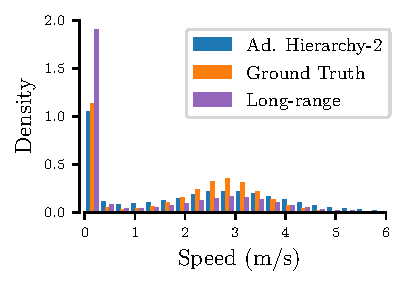
\includegraphics[width=0.6\textwidth]{figs/fdm/hist_new.pdf}
    \caption{Comparison of speed distributions measured from dataset videos with those measured from videos sampled by our model using two different sampling schemes. The ground-truth speeds are concentrated around $3m/s$ with some additional probability mass on zero. Videos sampled with Long-range have more mass at zero than is realistic. Sampling with Ad. Hierarchy-2 fixes this problem, although neither sampling scheme is as concentrated around $3m/s$ as the ground truth.}
    \label{fig:hist}
\end{figure}
The relative performance of different sampling schemes varies significantly between datasets as shown in \cref{tab:fdm-results-completion}. We report Fréchet Video Distances (FVDs)~\cite{unterthiner2018towards}, a measure of how similar sampled completions are to the test set, on all datasets. In addition on GQN-Mazes we we report the accuracy metric~\cite{saxena2021clockwork}, which classifies videos based on which rooms are visited and measures how often a completion is given the same class as the corresponding test video. For CARLA Town01 we report the previously described percentage outliers (PO) and Wasserstein distance (WD) metrics. 

We can broadly consider the aforementioned sampling schemes as either being in the ``autoregressive'' family (Autoreg and Long-range) or in the ``hierarchical'' family (the remainder). Those in the hierarchical family achieve significantly better FVDs~\cite{unterthiner2018towards} on GQN-Mazes. Our samples in the appendix suggest that this is related to the autoregressive methods ``forgetting'' the colours of walls after looking away from them for a short time. In contrast, for MineRL the autoregressive methods tend to achieve the best FVDs. This may relate to the fact that trajectories in MineRL tend to travel in straight lines through procedurally-generated ``worlds''\cite{guss2019minerl,saxena2021clockwork}, limiting the number of long-range dependencies. 
Finally on CARLA Town01 we notice qualitatively different behaviours from our autoregressive and hierarchical sampling schemes. The hierarchical
sampling schemes have a tendency to occasionally lose coherence and ``jump'' 
to different locations in the town. This is reflected by higher outlier percentages (OP) in \cref{tab:fdm-results-completion}. On the other hand the autoregressive schemes often stay stationary for unrealistically long times at traffic lights. This is reflected in the histogram of speeds in \cref{fig:hist}, which has a larger peak around zero than the ground truth. The high variance of the sampling scheme's relative performance over different datasets points to a strength of our method, which need only be trained once and then used to explore a variety of sampling schemes. Furthermore, we point out that the best FVDs in \cref{tab:fdm-results-completion} on all datasets were obtained using sampling schemes that could not be implemented using models trained in prior work, or over evenly spaced frames.

\paragraph{Comparison with baselines}
The related work most relevant to ours is the concurrent work of \citet{ho2022video}, who model 64-frame videos using two trained DMs. The first is a ``frameskip-4'' model trained to generate every fourth frame and the second is a ``frameskip-1'' model trained on sequences of nine consecutive frames and used to ``fill in'' the gaps between frames generated in the first stage. To compare against this approach, which we denote \textbf{VDM}, we train both a ``frameskip-4'' and a ``frameskip-1'' model with architectures identical to our own.\footnote{The VDM is concurrent work and, at the time of writing, without a code-release. Since we intend this primarily as a comparison against the VDM sampling scheme we do not reimplement their exact architecture and note that there are other differences including their approach to imputation.} Since VDM requires two trained DMs, we train it for more GPU-hours than FDM despite the fact that FDM is meta-learning over a far broader task distribution. We also compare against \textbf{TATS}~\citep{ge2022long}, which embeds videos into a discrete latent space before modelling them with a transformers, and the clockwork VAE (\textbf{CWVAE})~\citep{saxena2021clockwork}, a VAE-based model specifically designed to maintain long-range dependencies within video.

Both the diffusion-based methods, FDM and VDM, achieve significantly higher FVD scores than TATS and CWVAE. This may point toward the utility of diffusion models in general for modelling images and video. \Cref{tab:fdm-results-completion} also makes clear the main benefit of FDM over VDM: although there is no sampling scheme for FDM which always outperforms VDM, there is at least one sampling scheme that outperforms it on each dataset. This speaks to the utility of learning a flexible model like FDM that allows different sampling schemes to be experimented with after training.

\begin{table} %{r}{80mm}
  \small
  \caption{Evaluation of video completions by our method with sampling schemes optimised offline as described in \cref{sec:fdm-method}.  We mark with an asterisk ($^*$) the eight numbers which improve on the corresponding non-optimised sampling schemes and highlight in bold those that are better than any in \cref{tab:fdm-results-completion}.}
  \vspace{2mm}
  \label{tab:fdm-optimized}
  \centering
  \begin{tabular}{lllllllll}
    \toprule
     & \multicolumn{2}{c}{GQN-Mazes}  & \multicolumn{1}{c}{MineRL}  & \multicolumn{3}{c}{CARLA Town01} \\
    \cmidrule(r){2-3} \cmidrule(r){4-4} \cmidrule(r){5-7}
    Sampling scheme       & FVD     & Accuracy    &    FVD & FVD & WD & OP \\
    \midrule
    Opt. autoreg        & $53.6 \pm 1.2^*$            & $80.2 \pm 1.2^*$            & $\mathbf{257 \pm 6.8}^*$    &   $146^*$ & $0.452^*$ & $0.65$   \\
    Opt. hierarchy-2   & $\mathbf{51.1 \pm 1.3}^*$    & $\mathbf{84.6 \pm 0.7}^*$   & $320 \pm 7.0$    &   $124$ & $0.349$ & $4.11^*$   \\
    \bottomrule
  \end{tabular}
\end{table}

\paragraph{Optimised sampling schemes}
As mentioned in \cref{sec:fdm-method}, another advantage of FDM is that it makes possible a model- and dataset-specific optimisation procedure to determine which frames to condition on at each stage. \Cref{tab:fdm-optimized} shows the results when this procedure is used to create sampling schemes for different datasets. In the first row we show results where the latent frames are fixed to be those of the Autoreg sampling scheme, and in the second row the latent frames are fixed to match those of Hierarchy-2. On two of the three datasets the best results in \cref{tab:fdm-results-completion} are improved upon, showing the utility of this optimisation procedure.

\paragraph{Comparison with training on a single task}
Training a network with our distribution over training tasks could be expected to lead to worse performance on a single task than training specifically for that task. To test whether this is the case, we train an ablation of FDM with training tasks exclusively of the type used in our Autoreg sampling scheme, i.e. ``predict ten consecutive frames given the previous ten.'' Tested with the Autoreg sampling scheme, it obtained an FVD of $82.0$ on GQN-Mazes and $234$ on MineRL. As expected given the specialisation to a single task, this is better than when FDM is run with the Autoreg sampling scheme (obtaining FVDs of $86.4$ and $281$ respectively).

\paragraph{Ablation on training task distribution}
To test how important our proposed structured training distribution is to FDM's performance, we perform an ablation with a different task distribution that samples $\latindices$ and $\obsindices$ from uniform distributions instead of our proposed structured task distribution. 
We provide full details in the appendix, but report here that switching away form our structured training distribution made the FVD scores worse on all five tested sampling schemes on both GQN-Mazes and MineRL. The reduction in the average FVD was $31\%$ on GQN-Mazes and $52\%$ on MineRL. This implies that our structured training distribution has a significant positive effect.

\section{Related work}


There are a number of approaches in the literature which use VAEs rather than DMs for video modelling. \citet{babaeizadeh2017stochastic} use a VAE model which predicts frames autoregressively conditioned on a global time-invariant latent variable. A related approach by \citet{denton2018stochastic} also uses a VAE with convolutional LSTM architectures in both the encoder and decoder. Unlike \citet{babaeizadeh2017stochastic} the prior is learned and a different latent variable is sampled for each frame. \citet{babaeizadeh2021fitvid} use a VAE with one set of latent variables per frame and inter-frame dependencies tracked by a two-layer LSTM. Their architecture intentionally overfits to the training data, which when coupled with image augmentations techniques achieves SOTA on various video prediction tasks.  \citet{kim2019variational} use a variational RNN~\citep{chung2015recurrent} with a hierarchical latent space that includes binary indicator variables which specify how the video is divided into a series of subsequences. Both \citet{villegas2018hierarchical} and \citet{wichers2018learning} target long-term video prediction using a hierarchical variational LSTM architecture, wherein high-level features such as landmarks are predicted first, then decoded into low-level pixel space. The two approaches differ in that \citet{villegas2018hierarchical} requires ground truth landmark labels, while \cite{wichers2018learning} removes this dependence using an unsupervised adversarial approach. Fully GAN-based video models have also been proposed~\citep{aldausari2022video,clark2019adversarial} but generally suffer from ``low quality frames or low number of frames or both''~\citep{aldausari2022video}.

\section{Discussion}
%Our method is still slow to sample from. There are techniques to speed up sampling~\citep{salimans2022progressive,song2020denoising} but exploring them was outside the scope of this paper.

In this chapter we have defined and empirically explored a new method for generating photorealistic videos with long-range coherence that respects and efficiently uses fixed, finite computational resources.
Our approach outperforms prior work on long-duration video modelling as measured by quantitative and semantically meaningful metrics. By doing so it serves as evidence that, when our data is sufficiently complex and high-dimensional, the flexible diffusion framework and flexible generative models can be useful for creating better generative models even if we only care about a single task like video continuation. In addition, the model we have presented is applicable to far more tasks without further training. Such tasks include conditioning on every $n$th frame to enable temporal super-resolution, or conditioning on both the first and final frame (potentially yielding a ``visual'' controller which proposes a path between a current state and a specified goal). Preliminary attempts to run in FDM conditioned on a final frame in this way yielded inconsistent results but we believe that this could be a fruitful direction for further investigation. Another promising avenue for exploration is simply to design better sampling schemes. More automated techniques to optimise these sampling schemes, and even to make them adapt given the values of previously generated frames, could have further benefits. One limitation of FDM is that each frame it considers must be either fully observed or fully unobserved; this was acceptable for the tasks we considered but more recent work has found that removing this limitation enables new inpainting-style tasks~\citep{green2024semantically}.

\clearpage
\newtheorem{proposition}{Proposition}
\newtheorem{lemma}{Lemma}
\newtheorem{assumption}{Assumption}

\chapter{Flexible Diffusion on Varying Dimensionality Data}
\label{ch:tddm}

So far in this thesis we have described how to train a diffusion model to be flexibly conditioned on any subset of its dimensions at test time, and how to adapt such a model to high-dimensional video data with bounded compute resources. In this section we explore how to enable flexible conditioning in another scenario: when the data $\rvx$ that we wish to infer has unknown dimensionality. This can be an issue with molecular data, where the number of atoms could vary, or with video data, where the number of frames can vary. When defining a generative model over these data-types, it is necessary to model the number of dimensions along with the raw values of each of its dimensions (the state). Previous approaches to modelling such data have relied on first sampling the number of dimensions from the empirical distribution obtained from the training data, and then sampling data using a fixed dimension diffusion model (FDDM) conditioned on this number of dimensions~\cite{hoogeboom2022equivariant}. This works well for unconditional generative modelling. For conditional modelling, where the number of dimensions may depend on the observations, this approach does not apply and we are forced to first train an auxiliary model that predicts the number of dimensions given the observations~\cite{igashov2022equivariant}.

This approach to trans-dimensional generative modelling is fundamentally limited due to the complete separation of dimension generation and state value generation. A particular limitation is in the common use-case of conditional sampling from an unconditional diffusion model discussed in \cref{sec:other-methods-for-conditional-sampling}. Here, an unconditional diffusion model is trained that end-users can then easily and cheaply adapt to their task of interest through conditioning~\cite{song2020score, dhariwal2021diffusion, clip_guided_diffusion, zhang2023towards} without needing to perform any further training or fine-tuning of the model. In an FDDM, there is no way for the guidance to appropriately guide the dimension of the generated datapoint. This can lead to incorrect generations for datasets where the dimension greatly affects the nature of the datapoint created, which is common since e.g. small molecules have completely different properties to large molecules.

To generate data of varying dimensionality, we propose a jump diffusion based generative model that jointly generates both the dimension and the state. Our model can be seen as a unification of diffusion models which generate all dimensions in parallel with autoregressive type models which generate dimensions sequentially. We derive the model through constructing a forward noising process that adds noise and removes dimensions and a backward generative process that adds dimensions while removing noise. We depict both processes in \cref{fig:tddm-fig1}. We derive the optimum backward generative process as the time-reversal of the forward noising process and derive a novel learning objective to learn this backward process from data. We demonstrate the advantages of our method on molecular and video datasets finding our method achieves superior guided generation performance and produces more representative data interpolations across dimensions.

\begin{figure}
    \centering
    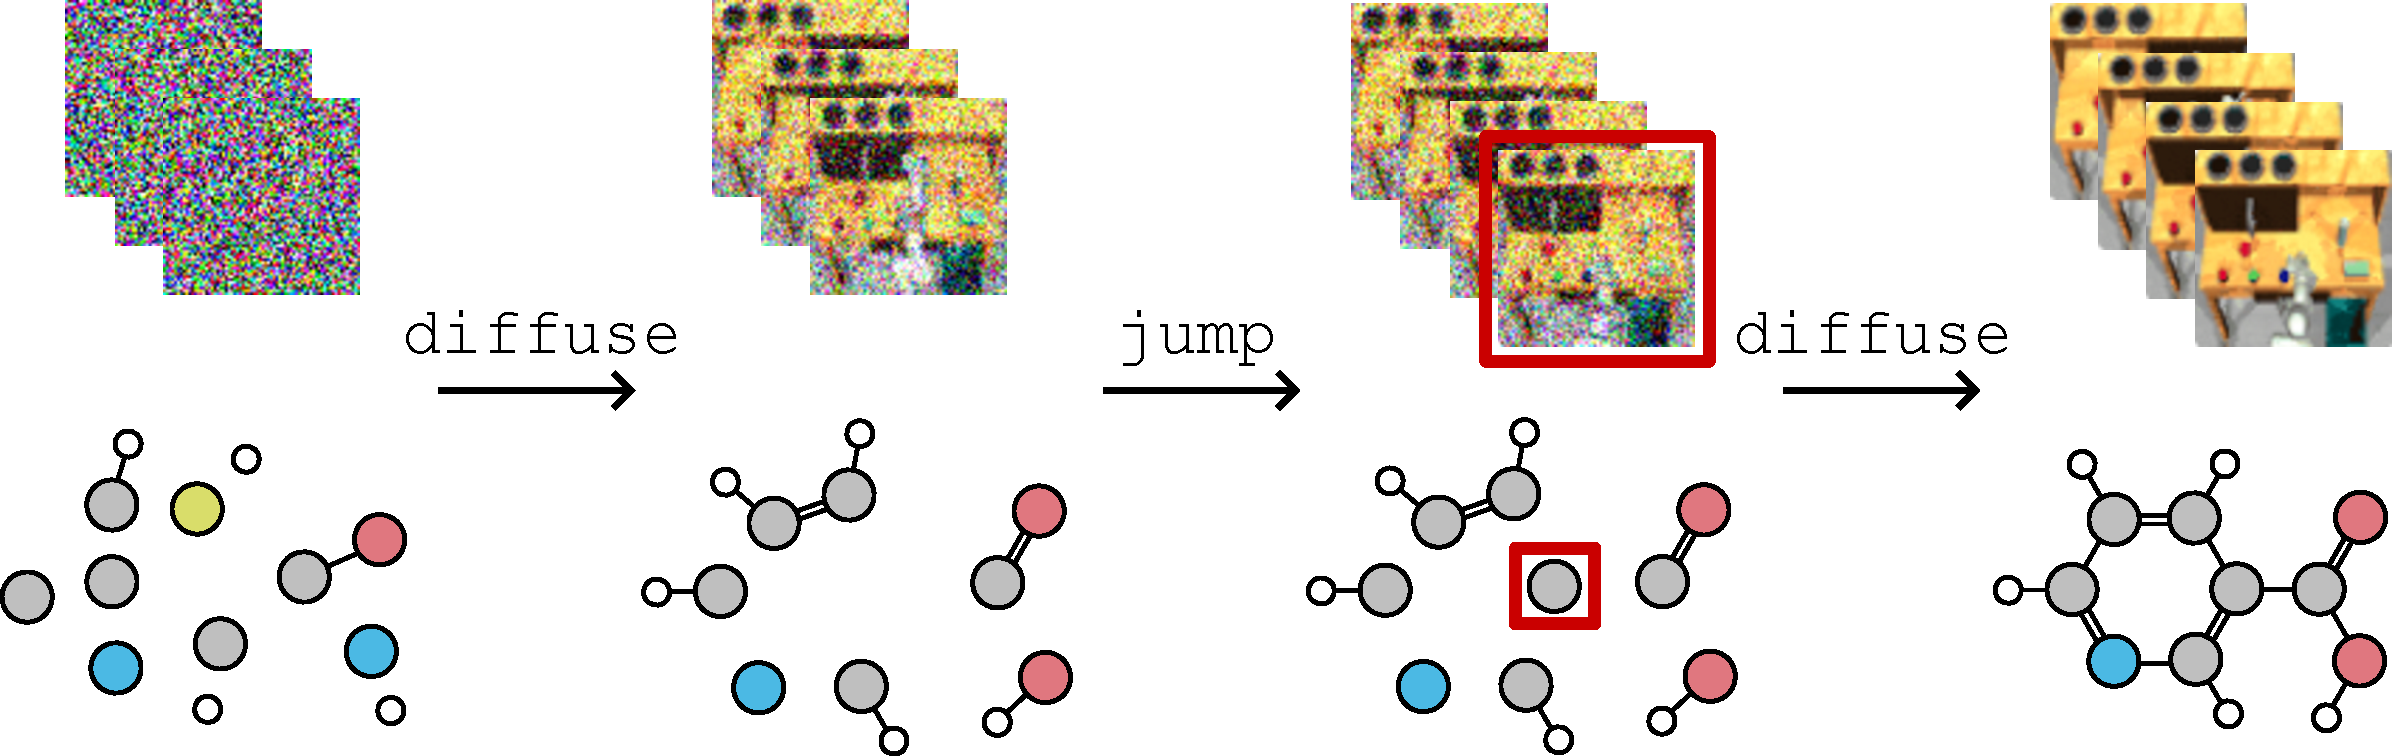
\includegraphics[width=\textwidth]{figs/tddm/fig1.pdf}
    \caption{Illustration of the jump diffusion generative process on videos and molecules. The generative process consists of two parts: a diffusion part which denoises the current set of frames/atoms and a jump part which adds on a suitable number of new frames/atoms such that the final generation is a clean synthetic datapoint of an appropriate size.
    }
    \label{fig:tddm-fig1}
\end{figure}


\section{Background}
Standard continuous-time diffusion models \cite{song2020score,huang2021variational,karraselucidating2022,benton2022denoising}  define a forward diffusion process through a stochastic differential equation (SDE) where $\rvx_0 \sim \pdata$ and, for $t>0$,
\begin{equation}\label{eq:forwardnoising}
     \rmd \rvx_t = \forwarddrift_t(\rvx_t) \rmd t + \diffcoeff_t \rmd \brown_t,
\end{equation}
where $\rvx_t \in \mathbb{R}^d$ is the current state, $\forwarddrift_t: \mathbb{R}^d \rightarrow \mathbb{R}^d$ is the drift and $\diffcoeff_t \in \mathbb{R}$ is the diffusion coefficient. $ \rmd \brown_t$ is a Brownian motion increment on $\mathbb{R}^d$. This SDE can be understood intuitively by noting that in each infinitesimal timestep, we move slightly in the direction of the drift $\forwarddrift_t$ and inject a small amount of Gaussian noised governed by $\diffcoeff_t$.
Let $p_t(\rvx_t)$ denote the distribution of $\rvx_t$ for the forward diffusion process \eqref{eq:forwardnoising} so that $p_0(\rvx_0) = \pdata(\rvx_0)$. $\forwarddrift_t$ and $\diffcoeff_t$ are set such that at time $t=T$, $p_T(\rvx_T)$ is close to $\pref(\rvx_T)= \mathcal{N}(\rvx_T;0, I_d)$; e.g. $\forwarddrift_t(\rvx_t)=-\frac{1}{2}g(t)^2 \rvx_t,$ for $g(t)>0$ \cite{ho2020denoising, song2020score}.

The time-reversal of the forward diffusion \eqref{eq:forwardnoising} is also a diffusion \cite{anderson1982reverse, haussmann1986time} which runs backwards in time from $p_T(\rvx_T)$ to $p_0(\rvx_0)$ and satisfies the following reverse time SDE
\begin{equation}
     \rmd \rvx_t = \backwarddrift_t(\rvx_t) \rmd t + \diffcoeff_t \rmd \hat{\brown}_t,
\end{equation}
where $\backwarddrift_t(\rvx_t) = \forwarddrift_t(\rvx_t) - \diffcoeff_t^2 \nabla_{\rvx_t} \log p_t(\rvx_t)$, $\rmd t$ is a negative infinitesimal time step and $\rmd \hat{\brown}_t$ is a Brownian motion increment when time flows backwards. 
Unfortunately, both the terminal distribution, $p_T(\rvx_T)$, and the score, $\nabla_{\rvx_t} \log p_{t}(\rvx_t)$, are unknown in practice.
A generative model is obtained by approximating $p_T$ with $\pref$ and learning an approximation $s^\theta_{t}(\rvx_t)$ to $\nabla_{\rvx_t} \log p_{t}(\rvx_t)$ typically using denoising score matching \cite{vincent2011connection}, i.e. 
\begin{equation}
    \underset{\theta}{\text{min}} \quad \mathbb{E}_{\mathcal{U}(t; 0, T) p_{0,t}(\rvx_0, \rvx_t)} [ \norm{s^\theta_t(\rvx_t) - \nabla_{\rvx_t} \log p_{t|0}(\rvx_t | \rvx_0)}^2 ].
    \label{eq:dsm}
\end{equation}
For a flexible model class, $s^\theta$, we get $s^\theta_t(\rvx_t) \approx \nabla_{\rvx_t} \log p_t(\rvx_t)$ at the minimizing parameter.

\section{Trans-Dimensional Generative Model}
Instead of working with fixed dimension datapoints, we will instead assume our datapoints consist of a variable number of components. A datapoint $\mX$ consists of $n$ components each of dimension $d$. For ease of notation, each datapoint will explicitly store both the number of components, $n$, and the state values, $\rvx$, giving $\mX = (n, \rvx)$. Since each datapoint can have a variable number of components from $n=1$ to $n=N$, our overall space that our datapoints live in is the union of all these possibilities, $\mX \in \gX = \bigcup_{n=1}^N \{n \} \times \mathbb{R}^{nd}$. For example, for a varying size point cloud dataset, components would refer to points in the cloud, each containing $(x,y,z)$ coordinates giving $d=3$ and the maximum possible number of points in the cloud is $N$.

Broadly speaking, our approach will follow the same framework as previous diffusion models. We will first define a forward noising process that both corrupts state values with Gaussian noise and progressively deletes dimensions.
We then learn an approximation to the time-reversal giving a backward generative process that simultaneously denoises whilst also progressively adding dimensions back until a synthetic datapoint of appropriate dimensionality has been constructed.

\subsection{Forward Process}
\label{sec:jump-diff-proc}

\todo{rename $\mY$ to avoid clash}
Our forward and backward processes will be defined through jump diffusions. A jump diffusion process has two components, the diffusion part and the jump part. Between jumps, the process evolves according to a standard SDE. When a jump occurs, the process transitions to a different dimensional space with the new value for the process being drawn from a transition kernel $K_t(\mY | \mX): \gX \times \gX \rightarrow  \mathbb{R}_{\geq 0}$. Letting $\mY = (m, \rvy)$, the transition kernel satisfies $\sum_m \int_\rvy K_t(m, \rvy | \mX) \rmd \rvy = 1$ and $\int_\rvy K_t(m=n, \rvy | \mX) \rmd \rvy = 0$. The rate at which jumps occur (jumps per unit time) is given by a rate function $\lambda_t(\mX): \mathcal{X} \rightarrow \mathbb{R}_{\geq 0}$. 
We can describe a jump diffusion in terms of an infinitesimal timestep $\rmd t$. For the forward process we call the transition kernel $\ftk_t(\mY|\mX)$ and rate function $\forwardrate_t(\mX_t)$. We will give their precise definitions shortly. Given this notation, we write the forward jump diffusion as
\begin{align}
    \textbf{Jump} \hspace{1cm} & \mX_t' = \begin{cases}
        \mX_t & \text{with probability } 1 - \forwardrate_t(\mX_t) \rmd t \\
        \mY \sim \ftk_t( \mY |\mX_t) & \text{with probability } \forwardrate_t(\mX_t) \rmd t
    \end{cases}  \label{eq:tddm-forward-jump} \\
    \textbf{Diffusion} \hspace{1cm} &\rvx_{t+ \rmd t} = \rvx'_t + b(t)\rvx'_t \rmd t + g(t) \rmd \brown_t \hspace{1cm} n_{t+\rmd t} = n_t'
     \label{eq:tddm-forward-diffusion}
\end{align}
with $\mX_t \triangleq (n_t, \rvx_t)$ and $\mX_{t+\rmd t} \triangleq (n_{t+\rmd t}, \rvx_{t + \rmd t})$ and $\rmd \brown_t$ being a Brownian motion increment on $\mathbb{R}^{n_t'd}$. We provide a more formal definition in Appendix \ref{sec:tddm-Proofs}.

With the jump diffusion formalism in hand, we can now construct our forward noising process. We will use the diffusion part to corrupt existing state values with Gaussian noise and the jump part to destroy dimensions. For the diffusion part, we use the variance-preserving diffusion SDE introduced in \cref{ch:diffusion}~\cite{ho2020denoising, song2020score} so $b(t) = -\frac{1}{2}g(t)^2$.

When a jump occurs in the forward process, one component of the current state will be deleted.
For example, one point in a point cloud or a single frame in a video is deleted. The rate at which these deletions occur is set by a user-defined forward rate $\smash{\forwardrate_t}(\mX)$. To formalise the deletion, we need to introduce some more notation. We let $\delidxdist(i | n)$ be a user-defined distribution over which component of the current state to delete. We also define $\text{del}: \mathcal{X} \times \mathbb{N} \rightarrow \mathcal{X}$ to be the deletion operator that deletes a specified component. Specifically, $(n-1, \rvy) = \text{del}((n, \x), i)$ where $\rvy \in \mathbb{R}^{(n-1)d}$ has the same values as $\x \in \mathbb{R}^{nd}$ except for the $d$ values corresponding to the $i$th component which have been removed. 
We can now define the forward jump transition kernel as $\ftk_t(\mY | \mX) = \sum_{i=1}^n \delidxdist (i | n) \updelta_{\text{del}(\mX, i)}(\mY)$. We note that only one
component is ever deleted at a time meaning $\ftk_t(m, \rvy | \mX) = 0$ for $m \neq n - 1$. Further, the choice of $\delidxdist(i | n)$ will dictate the behaviour of the reverse generative process. If we set $\delidxdist(i | n) = \mathbb{I}\{i=n\}$ then we only ever delete the final component and so in the reverse generative direction, datapoints are created additively, appending components onto the end of the current state. Alternatively, if we set $\delidxdist(i | n) = 1/n$ then components are deleted uniformly at random during forward corruption and in the reverse generative process, the model will need to pick the most suitable location for a new component from all possible positions.

The forward noising process is simulated from $t=0$ to $t=T$ and should be such that at time $t=T$, the marginal probability $p_t(\mX)$ should be close to a reference measure $\pref(\mX)$ that can be sampled from. 
We set $\pref(\mX) = \mathbb{I} \{ n = 1\} \mathcal{N}(\rvx; 0, I_{d})$ where $\mathbb{I} \{ n = 1\}$ is $1$ when $n=1$ and $0$ otherwise. To be close to $\pref$, for the jump part, we set $\forwardrate_t$ high enough such that at time $t=T$ there is a high probability that all but one of the components in the original datapoint have been deleted. For simplicity, we also set $\forwardrate_t$ to depend only on the current dimension $\forwardrate_t(\mX) = \forwardrate_t(n)$ with $\forwardrate_t(n=1) = 0$ so that the forward process stops deleting components when there is only $1$ left. In our experiments in \cref{sec:tddm-experiments} we demonstrate the trade-offs between different rate schedules in time. For the diffusion part, we use standard $g(t)$ schedules which ensure that we are close to $\mathcal{N}(\rvx; 0, I_{d})$.

\subsection{Backward Process}
The backward generative process will simultaneously denoise and add dimensions back in order to construct the final datapoint. Its drift term corresponds to that of a standard reverse diffusion SDE from \cref{ch:diffusion}, consisting of the sum of the forward drift term and a scaled score function. We will call the backwards rate function $\backwardrate_t(\mX)$ and the backwards transition kernel $\btk_t(\mY | \mX)$ and so write the jump diffusion as
\begin{align}
    \label{eq:tddm-reverse-jump}
    \textbf{Jump} \hspace{.4cm} & \mX_t' = \begin{cases}
        \mX_t & \text{with probability } 1 - \backwardrate_t(\mX_t) \rmd t \\
        \mY \sim \btk_t( \mY |\mX_t) & \text{with probability } \backwardrate_t(\mX_t) \rmd t
    \end{cases} 
    \\
    \label{eq:tddm-reverse-diffusion}
    \textbf{Diffusion} \hspace{.4cm} &\rvx_{t+ \rmd t} = \rvx'_t + \left(b(t)\rvx_t + g(t)^2 \rvs_\theta(\mX, t) \right) \rmd t + g(t) \rmd \brown_t \hspace{.5cm} n_{t+\rmd t} = n_t'
\end{align}
We would now like to specify the form of $\backwardrate_t(\mX)$ and $\btk(\mY|\mX)$, and ensure that these make the backward process the time-reversal of the forward process. 
% In order to find the time-reversal of the forward process, we must first introduce some notation to describe $\btk_t(\mY | \mX)$.
$\btk_t(\mY | \mX)$ should undo the forward deletion operation. Since $\ftk_t(\mY | \mX)$ chooses a component and then deletes it, $\btk_t(\mY | \mX)$ will need to generate the state values for a new component, decide where the component should be placed and then insert it at this location. 
Our new component will be denoted $\yadd \in \mathbb{R}^{d}$. 
The insertion operator is defined as $\text{ins}: \gX \times \mathbb{R}^{d} \times \mathbb{N} \rightarrow \gX$. It takes in the current value $\mX$, the new component $\yadd$ and an index $i \in \{1, \dots, n+1\}$ and inserts $\yadd$ into $\mX$ at location $i$ such that the resulting value $\mY = \text{ins}(\mX, \yadd, i)$ has $\text{del}(\mY, i) = \mX$.
We denote the joint conditional distribution over the newly added component and the index at which it is inserted as $\autonet_t(\yadd, i | \mX)$.
We therefore have $\btk_t(\mY | \mX) = \int_{\yadd} \sum_{i=1}^{n+1}  \autonet_t(\yadd, i | \mX) \updelta_{\text{ins}(\mX, \yadd, i)}(\mY) \rmd \yadd$. Noting that only one component is ever added at a time, we have $\btk_t(m, \rvy | \mX) = 0$ for $m \neq n+1$. 

This backward process formalism can be seen as a unification of diffusion models with autoregressive models. The diffusion part $\backwarddrift_t$ denoises the current set of components in parallel, whilst the autoregressive part $\autonet_t(\yadd, i | \mX)$ predicts a new component and its location. $\backwardrate_t(\mX)$ is the glue between these parts controlling when and how many new components are added during generation.

% \begin{table}
% \caption{Summary of forward and parameterized backward processes}
% \label{tab:forward_and_backward}
% \centering
% \small
% \begin{tabular}{@{}cccc@{}}
% \toprule
% Direction & $\drift_t$ & $\lambda_t(\mX)$ & $K_t(\mY | \mX)$ \\ \midrule
% \textbf{Forward} & $-\frac{1}{2} g(t)^2 \x$ & $\forwardrate_t(n)$ & $\sum_{i=1}^n \delidxdist(i | n) \updelta_{\text{del}(\mX, i)}(\mY)$ \\
% \textbf{Backward} & $ -\frac{1}{2} g(t)^2 \x - g(t)^2 s_{t}^\theta(\mX)$ & $\backwardrate_t^\theta(\mX)$ & $\int_{\yadd} \sum_{i=1}^{n+1}  \autonet^\theta_t(\yadd, i | \mX) \updelta_{\text{ins}(\mX, \yadd, i)}(\mY) \rmd \yadd$ \\ \bottomrule
% \end{tabular}
% \end{table}

The following proposition states the values for $\backwardrate_t(\mX)$ and $A_t(\yadd, i | \mX)$ which ensure that the backward process is the time-reversal of the forward process.
\begin{proposition}
\label{prop:time_reversal}
The time reversal of a forward jump diffusion process given by drift $b(t)$, diffusion coefficient $g(t)$, rate $\forwardrate_t(n)$ and transition kernel $\sum_{i=1}^n \delidxdist(i | n) \updelta_{\textup{del}(\mX, i)}(\mY)$ is given by a jump diffusion process with diffusion component as defined in \cref{eq:tddm-reverse-diffusion} and rate $\backwardrate_t^*(\mX)$ and transition kernel $\int_{\yadd} \sum_{i=1}^{n+1}  \autonet^*_t(\yadd, i | \mX) \updelta_{\textup{ins}(\mX, \yadd, i)}(\mY) \rmd \yadd$ as defined below
\begin{align}
    % &\backwarddrift_{t}^*(\mX) = \forwarddrift_{t}(\mX) - \forwarddiffcoeff_t^2 \nabla_{\x} \log p_{t}(\mX),~~\backwarddiffcoeff_{t}^* = \forwarddiffcoeff_{t},\\
    & \backwardrate_{t}^*(\mX) = \forwardrate_{t}(n+1) \frac{ \sum_{i=1}^{n+1} \delidxdist(i | n+1) \int_{\yadd} p_{t}( \textup{ins}(\mX, \yadd, i)) \rmd \yadd }{p_{t}(\mX)},\\
    & \autonet_{t}^*( \yadd, i | \mX) \propto p_{t}(\textup{ins}(\mX, \yadd, i) ) \delidxdist(i| n+1).
\end{align}
\end{proposition}
All proofs are given in Appendix~\ref{sec:tddm-Proofs}. The expressions for $\backwarddrift_t^*$ and $\backwarddiffcoeff^*_t$ are the same as for a standard diffusion except for replacing $\nabla_{\x} \log p_t(\x)$ with $\nabla_{\x} \log p_t(\mX) = \nabla_{\x} \log p_t(\x | n)$ which is simply the score in the current dimension.
The expression for $\backwardrate_t^*$ can be understood intuitively by noting that the numerator in the probability ratio is the probability that at time $t$, given a deletion occurs, the forward process will arrive at $\mX$. If this is higher than the raw probability at time $t$ that the forward process is at $\mX$ (the denominator) then we should have high $\backwardrate_t^*$ because $\mX$ is likely the result of a deletion of a larger datapoint.
Finally the optimum $\autonet^*_t(\yadd, i | \mX)$ is simply the conditional distribution of $\yadd$ and $i$ given $\mX$ when the joint distribution over $\yadd, i, \mX$ is given by $p_{t}(\text{ins}(\mX, \yadd, i) ) \delidxdist(i| n+1)$. 

\subsection{Objective for Learning the Backward Process}
The true $\backwarddrift_t^*$, $\backwardrate_t^*$ and $\autonet_t^*$ are unknown so we need to learn approximations to them, $\backwarddrift_t^\theta$, $\backwardrate_t^\theta$ and $\autonet_t^\theta$. 
To parameterise the diffusion component of the reverse process, we can follow the procedure used in a standard diffusion model to learn the score function $\rvs_\theta(\mX, t)$. To parameterise the jump component, which relies on an unknown optimal rate $\backwardrate_t^*$ and unknown distribution $\autonet_t^*$, we will need a novel objective to learn approximations to $\backwardrate_t^\theta$ and $\autonet_t^\theta$.
% Following Proposition \ref{prop:time_reversal}, we set $\backwarddrift_t^\theta(\mX) = \forwarddrift_t(\mX) - \forwarddiffcoeff_t^2 s_t^\theta(\mX)$ where $s_t^\theta(\mX)$ approximates $\nabla_{\x} \log p_t(\mX)$.

Standard diffusion models are trained using a denoising score matching loss which can be derived from maximising an evidence lower bound on the model probability for $ \mathbb{E}_{\pdata(\rvx_0)} [ \log p_0^\theta(\rvx_0) ]$ \cite{song2021maximum}.
We derive here an equivalent loss to learn $s_t^\theta$, $\smash{\backwardrate_t^\theta}$ and $\autonet_t^\theta$ for our jump diffusion process by leveraging the results of \cite{benton2022denoising} and \cite{cheridito2005equivalent}. Before presenting this loss, we first introduce some notation. Our objective for $s_t^\theta(\mX_t)$ will resemble denoising score matching \eqref{eq:dsm} but instead involve the conditional score $\nabla_{\rvx_t} \log p_{t|0}(\mX_t | \mX_0) = \nabla_{\rvx_t} \log p_{t|0}(\rvx_t | \mX_0, n_t)$. This is difficult to calculate directly due to a combinatorial sum over the different ways the components of $\mX_0$ can be deleted to get to $\mX_t$. We avoid this problem by equivalently conditioning on a mask variable $M_t \in \{0, 1\}^{n_0}$ that is 0 for components of $\mX_0$ that have been deleted to get to $\mX_t$ and 1 for components that remain in $\mX_t$. This makes our denoising score matching target easy to calculate: $\nabla_{\rvx_t} \log p_{t|0}(\rvx_t | \mX_0, n_t, M_t) = \frac{\sqrt{\alpha_t} M_t(\rvx_0) - \rvx_t}{1 - \alpha_t}$ where $\alpha_t = \text{exp} ( - \int_{0}^t g(t)^2 \rmd s )$ \cite{song2020score}. Here $M_t(\rvx_0)$ is the vector removing any components in $\rvx_0$ for which $M_t$ is $0$, thus $M_t(\rvx_0)$ and $\rvx_t$ have the same dimensionality. We now state our full objective.

\begin{proposition}
\label{prop:elbo}
For the backward generative jump diffusion process starting at $\pref(\mX_T)$ and finishing at $ p_0^\theta(\mX_0)$, an evidence lower bound on the model log-likelihood $ \mathbb{E}_{\rvx_0 \sim \pdata} [ \log p_0^\theta(\rvx_0) ]$ is given by
\begin{align}
    \label{eq:elbo_line_1}
    \mathcal{L}(\theta) = -\frac{T}{2} \mathbb{E}\Big[& \diffcoeff_t^2 \norm{s_t^\theta(\mX_t) - \nabla_{\rvx_t} \log p_{t|0}(\rvx_t | \mX_0, n_t, M_t)   }^2 \Big] + \\
    \label{eq:elbo_line_2}
    T \mathbb{E} \Big[& - \backwardrate_{t}^\theta(\mX_t) + \forwardrate_t (n_t) \log \backwardrate_{t}^\theta(\mY) + \forwardrate_t(n_t) \log \autonet_{t}^\theta(\xadd_t, i | \mY) \Big] + C,
\end{align}
where expectations are with respect to $\mathcal{U}(t; 0, T) p_{0,t}(\mX_0, \mX_t, M_t) \delidxdist(i | n_t) \updelta_{\textup{del}(\mX_t, i)} (\mY)$, $C$ is a constant term independent of $\theta$ and $\mX_t = \text{ins}(\mY, \xadd_t, i)$.
This evidence lower bound is equal to the log-likelihood when $\backwarddrift_t^\theta = \backwarddrift_t^*$, $\backwardrate_t^\theta = \backwardrate_t^*$ and $A_t^\theta = A_t^*$.

\end{proposition}


We now examine the objective to gain an intuition into the learning signal.
Our first term \eqref{eq:elbo_line_1} is an $L_2$ regression to a target that, as we have seen, is a scaled vector between $\rvx_t$ and $\sqrt{\alpha_t}M_t(\rvx_0)$.
As the solution to an $L_2$ regression problem is the conditional expectation of the target, $s_t^\theta(\mX_t)$ will learn to predict vectors pointing towards $\rvx_0$ averaged over the possible correspondences between dimensions of $\rvx_t$ and dimensions of $\rvx_0$.
Thus, during sampling, $s_t^\theta(\mX_t)$ provides a suitable direction to adjust the current value $\mX_t$ taking into account the fact $\mX_t$ represents only a noisy subpart of a clean whole $\mX_0$.

The second term (\ref{eq:elbo_line_2}) gives a learning signal for $\backwardrate_{t}^\theta$ and $\autonet_{t}^\theta$.
For $\autonet_{t}^\theta$, we simply have a maximum likelihood objective, predicting the missing part of $\mX_t$ (i.e.~$\xadd_t$) given the observed part of $\mX_t$ (i.e.~$\mY$).
The signal for $\backwardrate_{t}^\theta$ comes from balancing two terms: $-\backwardrate_{t}^\theta(\mX_t)$ and $\forwardrate_t(n_t) \log \backwardrate_{t}^\theta(\mY)$ which encourage the value of $\backwardrate_{t}^\theta$ to move in opposite directions. For a new test input $\mZ$, $\backwardrate_{t}^\theta(\mZ)$'s value needs to trade off between the two terms by learning the relative probability between $\mZ$ being the entirety of a genuine sample from the forward process, corresponding to the $\backwardrate_t^\theta(\mX_t)$ term in \eqref{eq:elbo_line_2}, or $\mZ$ being a substructure of a genuine sample, corresponding to the $\backwardrate_t^\theta(\mY)$ term in \eqref{eq:elbo_line_2}. The optimum trade-off is found exactly at the time reversal $\backwardrate_{t}^*$ as we show in Appendix \ref{sec:ObjTimeRevProof}.

We optimize $\mathcal{L}(\theta)$ using stochastic gradient ascent, generating minibatches by first sampling $t \sim \mathcal{U}(0, T)$, $\mX_0 \sim \pdata$ and then computing $\mX_t$ from  the forward process. This can be done analytically for the $\forwardrate_t(n)$ functions used in our experiments. We first sample $n_t$ by analytic integration of the dimension deletion Poisson process with time inhomogeneous rate $\forwardrate_t(n)$. We then add Gaussian noise independently to each dimension under $p_{t|0}(\rvx_t | \mX_0, n_t, M_t)$ using a randomly drawn mask variable $M_t$. See Appendix \ref{sec:ApdxTrainingObjective} for further details on the efficient evaluation of our objective.
\subsection{Parameterization}

$s_t^\theta(\mX_t)$, $\autonet_t^\theta(\yadd, i | \mX_t)$ and $\backwardrate_t^\theta(\mX_t)$ will all be parameterized by neural networks. In practice, we have a single backbone network suited to the problem of interest e.g. a Transformer \cite{vaswani2017attention}, an EGNN \cite{satorras2021n} or a UNet \cite{ronneberger2015u} onto which we add prediction heads for $s_t^\theta(\mX_t)$, $\autonet_t^\theta(\yadd, i | \mX_t)$ and $\backwardrate_t^\theta(\mX_t)$. $s_t^\theta(\mX_t)$ outputs a vector in $\mathbb{R}^{n_t d}$. $\autonet_t^\theta(\yadd, i | \mX_t)$ outputs a distribution over $i$ and mean and standard deviation statistics for a Gaussian distribution over $\yadd$. Finally, having $\backwardrate_t^\theta(\mX_t) \in \mathbb{R}_{\geq 0}$ be the raw output of a neural network can cause optimization issues due to the optimum $\backwardrate^*_t$ including a probability ratio which can take on very large values. Instead, we learn a component prediction network $p^\theta_{0|t}(n_0 | \mX_t)$ that predicts the number of components in $\mX_0$ given $\mX_t$. To convert this into $\backwardrate^\theta(\mX_t)$, we show in Proposition \ref{prop:backwardrateparam} how the optimum $\backwardrate_t^*(\mX_t)$ is an analytic function of the true $p_{0|t}(n_0 | \mX_t)$. We then plug $p^\theta_{0|t}(n_0 | \mX_t)$ into Proposition \ref{prop:backwardrateparam} to obtain an approximation of $\backwardrate_t^*(\mX_t)$.
\begin{proposition} We have
    \label{prop:backwardrateparam}
    \begin{equation}\label{eq:backwardrateparam}
        \backwardrate_{t}^*(\mX_t) = \forwardrate_{t}(n_t+1) \sum_{n_0=1}^N \frac{p_{t|0}(n_t + 1 | n_0)}{p_{t|0}(n_t | n_0)} p_{0|t}(n_0 | \mX_t),
    \end{equation}
    where $\mX_t = (n_t, \rvx_t)$ and $p_{t|0}(n_t + 1 | n_0)$ and $p_{t|0}(n_t | n_0)$ are both easily calculable distributions from the forward dimension deletion process.
\end{proposition}



\subsection{Sampling}

\begin{wrapfigure}{R}{0.6\textwidth}
    \begin{minipage}[t]{0.6\textwidth}
    \small
        \begin{algorithm}[H]
        \SetAlgoNoLine
        \DontPrintSemicolon
        $t \leftarrow T$\;
        $\mX \sim \pref(\mX) = \mathbb{I}\{ n=1\} \mathcal{N}(\x; 0, I_{d})$\;
        \While{ $t > 0$}{
        \If{$u < \backwardrate_{t}^\theta(\mX) \updelta t$~\textup{with~}$u \sim \mathcal{U}(0, 1)$}{
        Sample $\xadd, i \sim \autonet_{t}^\theta(\xadd, i | \mX)$ \;
        $\mX \leftarrow \text{ins}(\mX, \xadd, i)$\;
        }
        $\x \leftarrow \x - \backwarddrift_{t}^\theta(\mX) \updelta t + g(t) \sqrt{\updelta t} \epsilon$ with $\epsilon \sim \mathcal{N}(0, I_{nd})$ \;
        $\mX \leftarrow (n, \x)$, $t \leftarrow t - \updelta t$
        }
         \caption{Sampling the Generative Process}
         \label{alg:backwardsampling}
        \end{algorithm}
    \end{minipage}
\end{wrapfigure}
To sample the generative process, we numerically integrate the learned backward jump diffusion process using time-step  $\updelta t$. Intuitively, it is simply the standard continuous time diffusion sampling scheme \cite{song2020score} but at each timestep we check whether a jump has occurred and if it has, sample the new component and insert it at the chosen index as explained by Algorithm \ref{alg:backwardsampling}.


\section{Related Work}

Our method jointly generates both dimensions and state values during the generative process whereas prior approaches \cite{hoogeboom2022equivariant, igashov2022equivariant} are forced to first sample the number of dimensions and then run the diffusion process in this fixed dimension. When diffusion guidance is applied to these unconditional models \cite{weiss2023guided, zhang2023towards}, users need to pick by hand the number of dimensions independent of the conditioning information even though the number of dimensions can be correlated with the conditioning parameter.


Instead of automatically learning when and how many dimensions to add during the generative process, previous work focusing on images \cite{jing2022subspace, zhang2022dimensionality} hand pick dimension jump points such that the resolution of images is increased during sampling and reaches a certain pre-defined desired resolution at the end of the generative process. Further, rather than using any equivalent of $\autonet_t^\theta$, the values for new dimensions are simply filled in with Gaussian noise. These approaches mainly focus on efficiency rather than flexible generation as we do here.


The first term in our learning objective in Proposition \ref{prop:elbo} corresponds to learning the continuous part of our process (the diffusion) and the second corresponds to learning the discrete part of our process (the jumps). The first term can be seen as a trans-dimensional extension of standard denoising score matching \cite{vincent2011connection} whilst the second bears similarity to the discrete space ELBO derived in \cite{campbell2022continuous}.

Finally, jump diffusions also have a long history of use in Bayesian inference, where one aims to draw samples from a trans-dimensional target posterior distribution based on an unnormalized version of its density \cite{grenander1994representations}: an ergodic jump diffusion is designed which admits the target as the invariant distribution \cite{grenander1994representations,phillips1995bayesian,miller1997automatic}. The invariant distribution is not preserved when time-discretizing the process.
However, it was shown in  \cite{green1995reversible,green2003trans} how general jump proposals could be built and how this process could be ``Metropolized'' to obtain a discrete-time Markov process admitting the correct invariant distribution, yielding the popular Reversible Jump Markov Chain Monte Carlo algorithm.
Our setup differs significantly as we only have access to samples in the form of data, not an unnormalized target.


\section{Experiments} \label{sec:tddm-experiments}

\subsection{Molecules}
We now show how our model provides significant benefits for diffusion guidance and interpolation tasks. We model the QM9 dataset \cite{ruddigkeit2012enumeration, ramakrishnan2014quantum} of 100K varying size molecules. Following \cite{hoogeboom2022equivariant}, we consider each molecule as a 3-dimensional point cloud of atoms, each atom having the features: $(x,y,z)$ coordinates, a one-hot encoded atom type, and an integer charge value. Bonds are inferred from inter-atomic distances. We use an EGNN \cite{satorras2021n} backbone with three heads to predict $\smash{s_{t}^\theta}$, $\smash{p_{0|t}^\theta(n_0 | \mX_t)}$, and $\smash{\autonet_t^\theta}$. We uniformly delete dimensions, $K^{\text{del}}(i | n) = 1/n$, and since a point cloud is permutation invariant, $\smash{\autonet_t^\theta(\yadd | \mX_t)}$ need only predict new dimension values. We set $\smash{\forwardrate_t}$ to a constant except for $t < 0.1T$, where we set $\smash{\forwardrate_{t < 0.1T} = 0}$. This ensures that all dimensions are added with enough generation time remaining for the diffusion process to finalize all state values. 

We visualize sampling from our learned generative process in Figure \ref{fig:tddm-uncond_chain_vis}; note how the process jointly creates a suitable number of atoms whilst adjusting their positions and identities. Before moving on to apply diffusion guidance which is the focus of our experiments, we first verify our unconditional sample quality in Table \ref{tab:uncond_mol} and find we perform comparably to the results reported in \cite{hoogeboom2022equivariant} which use an FDDM. We ablate our choice of $\smash{\forwardrate_t}$ by comparing with setting $\smash{\forwardrate_t}$ to a constant for all $t$ and with setting $\smash{\forwardrate_t}=0$ for $t<0.9T$ (rather than just for $t<0.1T$). We find that the constant $\smash{\forwardrate_t}$ performs worse due to the occasional component being added late in the generation process without enough time for the diffusion process to finalize its value. We find the $\smash{\forwardrate_{t<0.9T} = 0}$ setting to have satisfactory sample quality however this choice of $\smash{\forwardrate_t}$ introduces issues during diffusion guided generation as we see next. Finally, we ablate the parameterization of Proposition \ref{prop:backwardrateparam} by learning $\backwardrate_t^\theta(\mX_t) \in \mathbb{R}$ directly as the output of a neural network head. We find that this reduces sample quality due to the more well-behaved nature of the target, $p_{0|t}^\theta(n_0 | \mX_t)$ when using Proposition \ref{prop:backwardrateparam}. We note pure autoregressive models perform significantly worse than diffusion based models as found in \cite{hoogeboom2022equivariant}.

\begin{figure}[h]
    \centering
    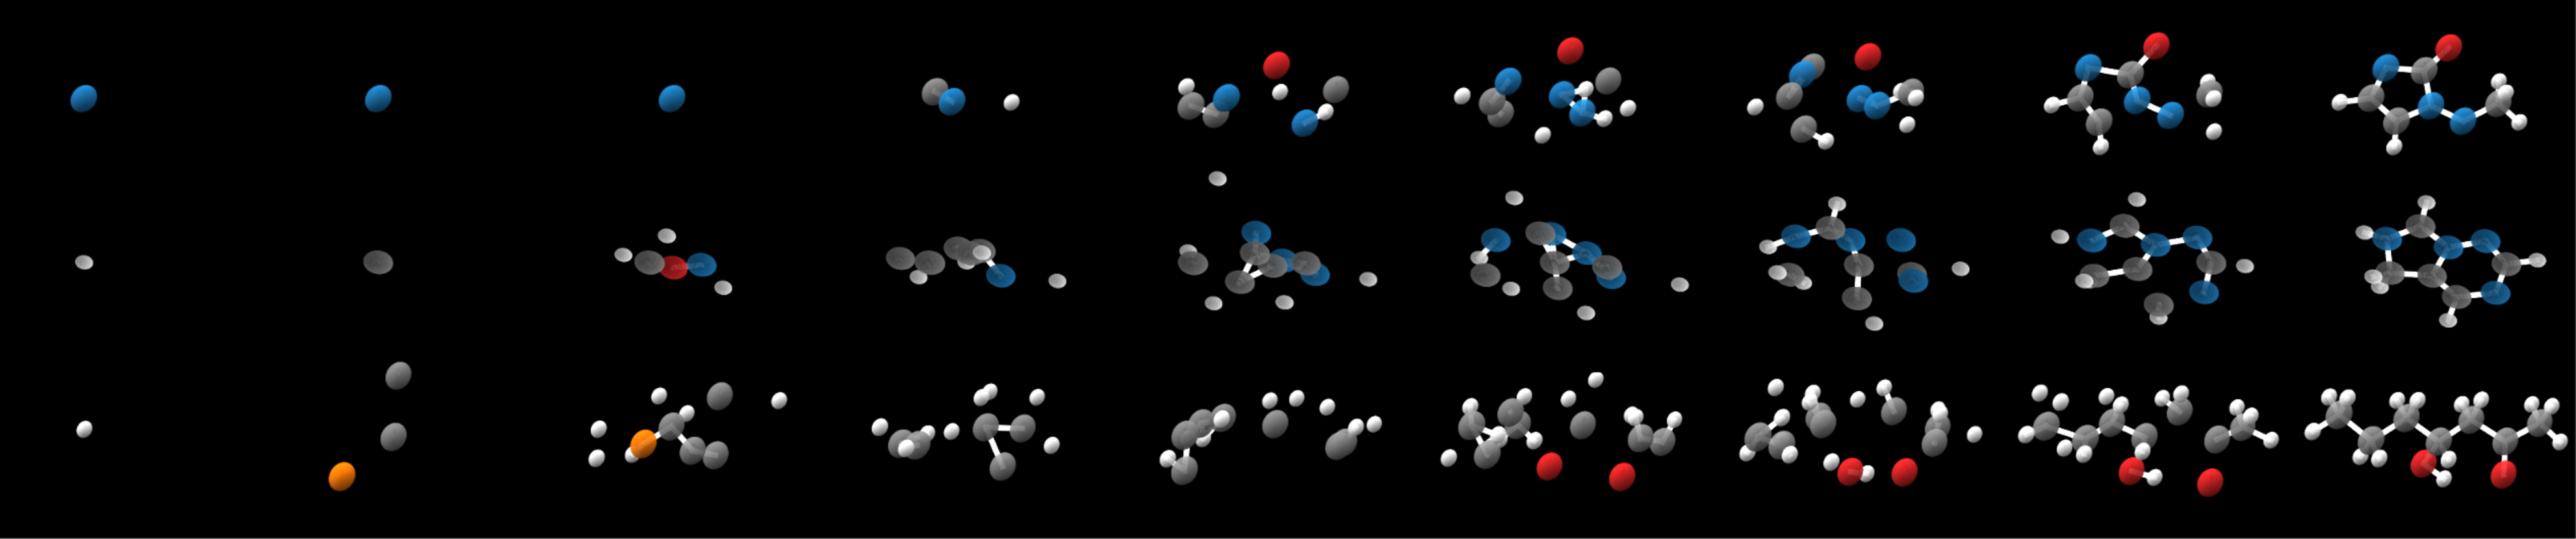
\includegraphics[width=\textwidth]{figs/tddm/genprog.pdf}
    \caption{Visualization of the jump-diffusion backward generative process on molecules.}
    \label{fig:tddm-uncond_chain_vis}
\end{figure}


\begin{table}[tb]
\caption{Sample quality metrics for unconditional molecule generation. An atom is stable if it has the correct valency whilst a molecule is considered stable if all of its atoms are stable. Molecular validity is measured using RDKit \cite{rdkit}. All methods use 1000 simulation steps and draw 10000 samples.}
\label{tab:uncond_mol}
\centering
\begin{tabular}{@{}lccc@{}}
\toprule
Method & \shortstack{\% Atom \\ Stable ($\uparrow$)} & \shortstack{ \% Molecule \\ Stable ($\uparrow$)} & \% Valid ($\uparrow$) \\ \midrule
FDDM \cite{hoogeboom2022equivariant} & $\mathbf{98.7}$ & $82.0$ & $91.9$  \\ \midrule
TDDM (ours) & $98.3$  & $\mathbf{87.2}$ & $\mathbf{92.3}$ \\
TDDM, const $\smash{\forwardrate_t}$ & $96.7$ & $79.1$ & $86.7$ \\
TDDM, $\smash{\forwardrate_{t<0.9T} = 0}$ & $97.7$ & $82.6$ & $89.4$ \\
TDDM w/o Prop. \ref{prop:backwardrateparam} & $97.0$ & $66.9$ & $87.1$ \\ \bottomrule
\end{tabular}
\end{table}
 

\subsubsection{Trans-Dimensional Diffusion Guidance}
\label{sec:mol_diff_guide}
We now apply diffusion guidance to our unconditional model in order to generate molecules that contain a certain number of desired atom types, e.g. 3 carbons or 1 oxygen and 2 nitrogens. The distribution of molecule sizes changes depending on these conditions. We generate molecules conditioned on these properties by using the reconstruction guided sampling approach introduced in \cite{ho2022video}. This method augments the score $s_{t}^\theta(\mX_t)$ such that it approximates $\nabla_{\rvx_t} \log p_{t}(\mX_t | y)$ rather than $\nabla_{\rvx_t} \log p_{t}(\mX_t)$ (where $y$ is the conditioning information) by adding on a term approximating $\nabla_{\rvx_t} \log p_{t}(y | \mX_t)$ with $p_t(y | \mX_t) = \sum_{n_0} \int_{\rvx_0} p(y | \mX_0) p_{0|t}(\mX_0 | \mX_t) \rmd \rvx_0 $. This guides $\rvx_t$ such that it is consistent with $y$. Since $\smash{\backwardrate_t^\theta(\mX_t)}$ has access to $\rvx_t$, it will cause $n_t$ to automatically also be consistent with $y$ without the user needing to input any information on how the conditioning information relates to the size of the datapoints. We give further details on diffusion guidance in Appendix \ref{sec:ApdxDiffGuide}.

\begin{table}[tb]
\caption{Conditional Molecule Generation for 10 conditioning tasks that each result in a different dimension distribution. We report dimension error as the average Hellinger distance between the generated and ground truth dimension distributions for that property as well as average sample quality metrics. Standard deviations are given across the 10 conditioning tasks. We report in bold values that are statistically indistinguishable from the best result at the $5\%$ level using a two-sided Wilcoxon signed rank test across the 10 conditioning tasks.}
\label{tab:cond_mol}
\centering
\begin{tabular}{@{}lcccc@{}}
\toprule
Method & \shortstack{Dimension \\ Error ($\downarrow$) } & \shortstack{ \% Atom \\ Stable ($\uparrow$)} & \shortstack{\% Molecule \\ Stable ($\uparrow$)} & \% Valid ($\uparrow$) \\ \midrule
FDDM & $0.511 {\scriptstyle \pm 0.19}$ & $93.5 {\scriptstyle \pm 1.1}$ & $31.3 {\scriptstyle \pm 6.3}$ & $65.2 {\scriptstyle \pm 10.3}$ \\ \midrule
TDDM  & $\mathbf{0.134 {\scriptstyle \pm 0.076}}$ & $93.5 {\scriptstyle \pm 2.6}$ & $\mathbf{59.1 {\scriptstyle \pm 11}}$ & $\mathbf{74.8 {\scriptstyle \pm 9.3}} $ \\
 TDDM, const $\smash{\forwardrate_t}$ & $0.226 {\scriptstyle \pm 0.17}$ & $88.9 {\scriptstyle \pm 4.8}$   & $43.6 {\scriptstyle \pm 15}$ & $63.4 {\scriptstyle \pm 14}$ \\
 TDDM, $\smash{\forwardrate_{t<0.9T} = 0}$&  $0.390 {\scriptstyle \pm 0.38}$& $\mathbf{95.0 {\scriptstyle \pm 2.1}}$& $\mathbf{61.7 {\scriptstyle \pm 17}}$ & $\mathbf{77.8 {\scriptstyle \pm 13}} $ \\
 TDDM w/o Prop. \ref{prop:backwardrateparam} & $0.219 {\scriptstyle \pm 0.12} $ & $\mathbf{93.8 {\scriptstyle \pm 3.2}}$ & $55.0 {\scriptstyle \pm 19}$ & $73.8 {\scriptstyle \pm 13}$  \\ \bottomrule
\end{tabular}
\end{table}

We show our results in Table \ref{tab:cond_mol}. In order to perform guidance on the FDDM baseline, we implement the model from \cite{hoogeboom2022equivariant} in continuous time and initialise the dimension from the empirically observed dimension distribution in the dataset.  This accounts for the case of an end user attempting to guide a unconditional model with access to no further information. We find that TDDM produces samples whose dimensions much more accurately reflect the true conditional distribution of dimensions given the conditioning information.
The $\forwardrate_{t<0.9T} = 0$ ablation on the other hand only marginally improves the dimension error over FDDM because all dimensions are added in the generative process at a time when $\mX_t$ is noisy and has little relation to the conditioning information. This highlights the necessity of allowing dimensions to be added throughout the generative process to gain the trans-dimensional diffusion guidance ability. The ablation with constant $\forwardrate_t$ has increased dimension error over TDDM as we find that when $\forwardrate_t > 0$ for all $t$, $\backwardrate_t^\theta$ can become very large when $t$ is close to 0 when the model has perceived a lack of dimensions. This occasionally results in too many dimensions being added hence an increased dimension error. Not using the Proposition \ref{prop:backwardrateparam} parameterisation also increases dimension error due to the increased difficulty in learning $\backwardrate_t^\theta$.

\begin{wrapfigure}{r}{0.5\textwidth}
    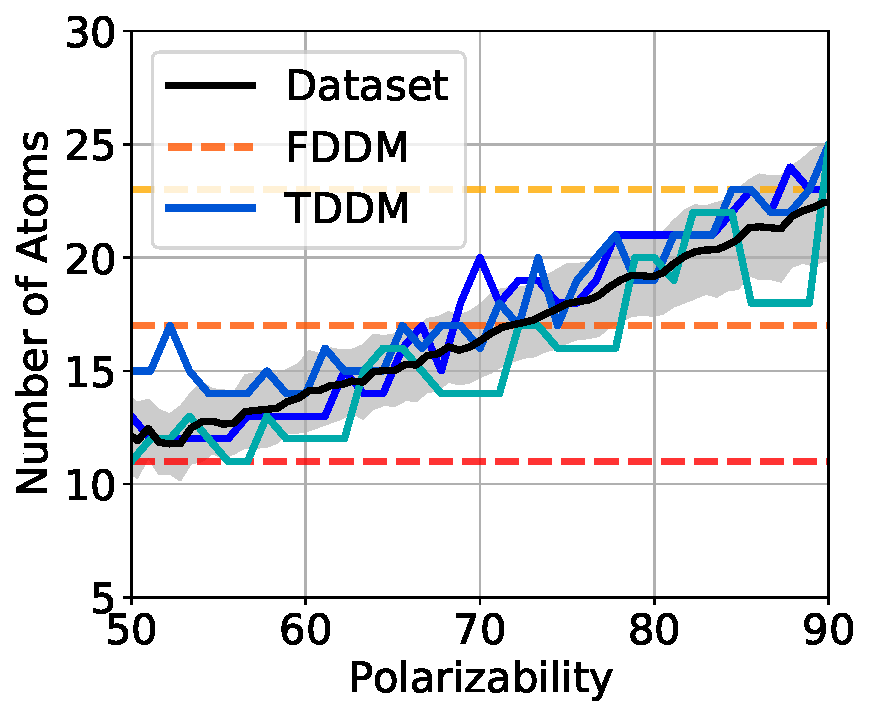
\includegraphics[width=0.35\textwidth]{figs/tddm/polarizability_vs_num_atoms.pdf}
    \caption{Number of atoms versus polarizability for $3$ interpolations with fixed random noise. The dataset mean and standard deviation for the number of atoms is also shown.
    FDDM interpolates entirely in a fixed dimensional space hence the number of atoms is fixed for all polarizabilities.}
    \label{fig:tddm-interp_plot}
\end{wrapfigure}

\subsubsection{Trans-Dimensional Interpolation}
\label{sec:mol_interp}
Interpolations are a unique way of gaining insights into the effect of some conditioning parameter on a dataset of interest.
To create an interpolation, a conditional generative model is first trained and then sampled with a sweep of the conditioning parameter but using fixed random noise \cite{hoogeboom2022equivariant}.
The resulting series of synthetic datapoints share similar features due to the fixed random noise but vary in ways that are very informative as to the effect of the conditioning parameter. 
Attempting to interpolate with an FDDM is fundamentally limited because the entire interpolation occurs in the same dimension which is unrealistic when the conditioning parameter is heavily correlated with the dimension of the datapoint. We demonstrate this by following the setup of \cite{hoogeboom2022equivariant} who train a conditional FDDM conditioned on polarizability.
Polarizability is the ability of a molecule's electron cloud to distort in response to an external electric field \cite{modernphysicalorganicchemistry} with larger molecules tending to have higher polarizability. To enable us to perform a trans-dimensional interpolation, we also train a conditional version of our model conditioned on polarizability. An example interpolation with this model is shown in Figure \ref{fig:tddm-interp}. We find that indeed the size of the molecule increases with increasing polarizability, with some molecular substructures e.g.~rings, being maintained across dimensions.
We show how the dimension changes with polarizability during 3 interpolations in Figure \ref{fig:tddm-interp_plot}. We find that these match the true dataset statistics much more accurately than interpolations using FDDM which first pick a dimension and carry out the entire interpolation in that fixed dimension.

\begin{figure}[h]
    \centering
    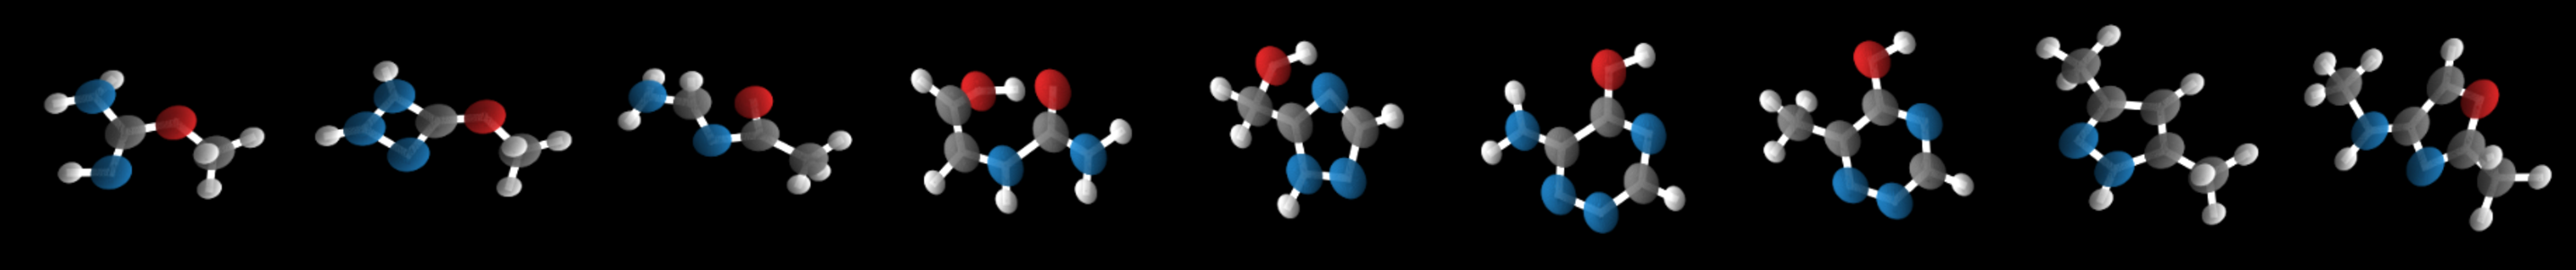
\includegraphics[width=\textwidth]{figs/tddm/small_interp_bright.pdf}
    \caption{Sequence of generations for linearly increasing polarizability from $39 \, \text{Bohr}^3$ to $66 \, \text{Bohr}^3$ with fixed random noise. Note how molecular size generally increases with polarizability and how some molecular substructures are maintained between sequential generations of differing dimension. For example, between molecules 6 and 7, the single change is a nitrogen (blue) to a carbon (gray) and an extra hydrogen (white) is added to maintain the correct valency.}
    \label{fig:tddm-interp}
\end{figure}



\subsection{Video}

We finally demonstrate our model on a video modelling task. Specifically we model the RoboDesk dataset~\citep{tian2023control}, a video benchmark to measure the applicability of video models for planning and control problems. The videos are renderings of a robotic arm~\citep{kannan2021robodesk} performing a variety of different tasks including opening drawers and moving objects.
We first train an unconditional model on videos of varying length and then perform planning by applying diffusion guidance to generate videos conditioned on an initial starting frame and a final goal frame \cite{janner2022diffuser}. The planning problem is then reduced to ``filling in'' the frames in between. Our trans-dimensional model automatically varies the number of in-filled frames during generation so that the final length of video matches the length of time the task should take, whereas the fixed dimension model relies on the unrealistic assumption that the length of time the task should take is known before generation.

We model videos at $32 \times 32$ resolution and with varying length from $2$ to $35$ frames. For the network backbone, we use a UNet adapted for video \cite{harvey2022flexible}. In contrast to molecular point clouds, our data is no longer permutation invariant hence $A_t^\theta(\yadd, i | \mX_t)$ includes a prediction over the location to insert the new frame. Full experimental details are provided in Appendix \ref{sec:ExperimentDetails}.
We evaluate our approach on three planning tasks, holding stationary, sliding a door and pushing an object. An example generation conditioned on the first and last frame for the slide door task is shown in Figure \ref{fig:tddm-video_example}, with the model in-filling a plausible trajectory. We quantify our model's ability to generate videos of a length appropriate to the task in Table \ref{tab:video_results} finding on all three tasks we generate a more accurate length of video than FDDM which is forced to sample video lengths from the unconditional empirically observed length distribution in the training dataset.

\definecolor{videored}{HTML}{f00606}
\definecolor{videoblue}{HTML}{4b4bfc}

\begin{figure}[h]
    \centering
    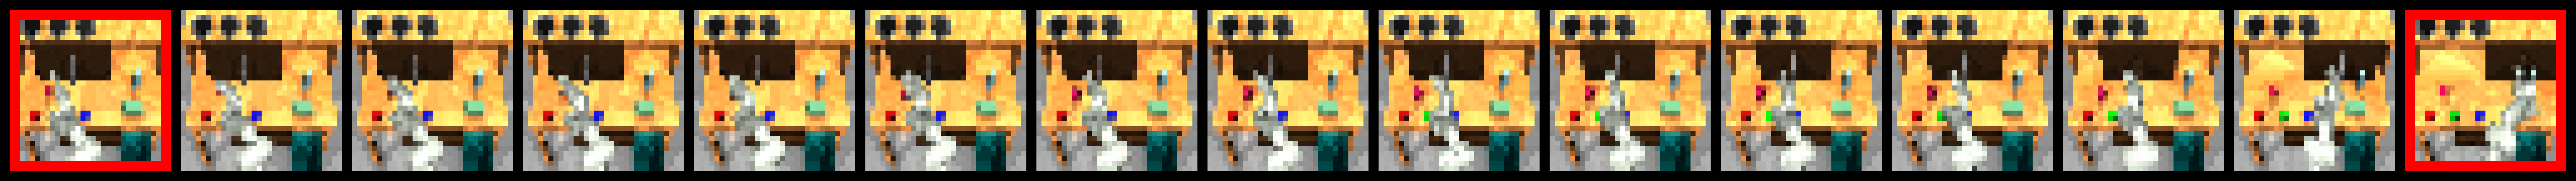
\includegraphics[width=\textwidth]{figs/tddm/21-1-padded_red_big.png}
    \caption{A sample for the slide door task conditioned on the first and last frame ({\color{red} highlighted}).}
    \label{fig:tddm-video_example}
\end{figure}

\begin{table}[h]
     \centering
   \caption{Dimension prediction mean absolute error for three planning tasks with standard deviations estimated over 45 samples.}
   \begin{tabular}{@{}lcccc@{}}
     \toprule
     Method & Stationary ($\downarrow$) & Slide Door ($\downarrow$) & Push Object ($\downarrow$) & Average ($\downarrow$)   \\ \midrule
     FDDM & $14.16 {\scriptstyle \pm 1.41}$ & $13.39 {\scriptstyle \pm 1.34}$ & $17.06 {\scriptstyle \pm 1.47}$ & $14.87$ \\
     TDDM & $\mathbf{9.70 {\scriptstyle \pm 0.99}}$ & $\mathbf{11.47 {\scriptstyle \pm 0.74}}$ & $\mathbf{15.43 {\scriptstyle \pm 0.90}}$ & $\mathbf{12.2}$ \\ \bottomrule
   \end{tabular}
   \label{tab:video_results}
\end{table}


\section{Discussion}
In this work, we highlighted the pitfalls of performing generative modelling on varying dimensional datasets when treating state values and dimensions completely separately. We instead proposed a trans-dimensional generative model that generates both state values and dimensions jointly during the generative process. We detailed how this process can be formalised with the time-reversal of a jump diffusion and derived a novel evidence lower bound training objective for learning the generative process from data. In our experiments, we found our trans-dimensional model to provide significantly better dimension generation performance for  diffusion guidance and interpolations when conditioning on properties that are heavily correlated with the dimension of a datapoint. We believe our approach can further enable generative models to be applied in a wider variety of domains where previous restrictive fixed dimension assumptions have been unsuitable.
\clearpage
\chapter{Flexible Variational Auto-Encoders}

\section{A Review of Variational Auto-Encoders}
\label{sec:vae}
As we did with diffusion models in \cref{ch:diffusion}, we will start by reviewing variational auto-encoders, or VAEs~\citep{kingma2013auto,rezende2014stochastic}, as unconditional generative models. We will then explain a conditional variant in \cref{sec:conditional-vae}. Like a diffusion model a variational auto-encoder is trained, using samples from a data distribution $\pdata(\rvx)$, to approximate $\pdata(\rvx)$. Given a variational auto-encoder with parameters $\theta$, we will denote the distribution it parameterises $p_\theta(\rvx)$. The key feature of a VAE is that it breaks the process of generating data into two steps: in the first step a VAE samples a latent variable $\rvz$ from a ``prior'' distribution $p_\theta(\rvz)$. The prior distribution can be fixed, \eg a unit Gaussian, or can have learnable parameters that are included in $\theta$. In the second step, the VAE parameterises a ``likelihood'' $p_\theta(\rvx|\rvz)$. This can be, \eg, a Gaussian for continuous data~\citep{kingma2013auto} or a categorical for discrete data~\citep{child2020very}, with parameters output in either case by a neural network as a function of $\rvz$. We can therefore write the parameterised distribution $p_\theta(\rvx)$ as the marginal of $p_\theta(\rvx|\rvz)$ over the latent variable $\rvz$,
% that is $p_\theta(\rvx) = \int p_\theta(\rvx|\rvz) p_\theta(\rvz) \mathrm{d}\rvz$.
\begin{equation} \label{eq:vae-marginal}
p_\theta(\rvx) = \int p_\theta(\rvx|\rvz)p_\theta(\rvz) \mathrm{d}\rvz.
\end{equation}
Even if both the prior $p_\theta(\rvz)$ and likelihood $p_\theta(\rvx|\rvz)$ are simple distributions, the marginal $p_\theta(\rvx)$ can be complex since the likelihood can be given by an arbitrarily complex function of $\rvz$.

As we discussed for diffusion models in \cref{ch:diffusion}, an ideal training objective would maximise the data likelihood $p_\theta(\rvx)$ averaged over all training examples since this corresponds to learning parameters which maximise the likelihood of the dataset under the learned distribution. The required marginalisation in \cref{eq:vae-marginal}, however, means that directly estimating the data likelihood is intractable. Therefore, as for diffusion models, we instead derive a training objective that lower-bounds the data likelihood. Starting by taking an expectation of the log of the data likelihood in \cref{eq:vae-marginal}, we can obtain a lower-bound using a proposal distribution $q_\phi(\rvz|\rvx)$ which can be given by a neural network with parameters $\phi$: % our objective can be converted to the log of an expectation over $q_\phi(\rvz)$:
\begin{align}
    \EX_{\pdata(\rvx)} \left[ \log p_\theta(\rvx) \right] &= \EX_{\pdata(\rvx)} \left[ \log \int p_\theta(\rvx|\rvz)p_\theta(\rvz) \mathrm{d}\rvz \right] \\
    &= \EX_{\pdata(\rvx)} \left[ \log \int p_\theta(\rvx|\rvz) \frac{p_\theta(\rvz)}{q_\phi(\rvz|\rvx)} q_\phi(\rvz|\rvx) \mathrm{d}\rvz \right] \\
    &= \EX_{\pdata(\rvx)} \left[ \log \EX_{q_\phi(\rvz|\rvx)} \left[ p_\theta(\rvx|\rvz) \frac{p_\theta(\rvz)}{q_\phi(\rvz|\rvx)} \right] \right]. \label{eq:vae-marginal-is}
\end{align}
Ideally we would be able to obtain an unbiased estimate of this objective. Due to the logarithm operator outside an intractable expectation this is not feasible but, using Jensen's inequality, we can obtain a training objective that lower bounds it by switching their order: 
\begin{align}
    \gL(\theta, \phi) := \EX_{\pdata(\rvx)q_\phi(\rvz|\rvx)} \left[ \log p_\theta(\rvx|\rvz) + \log \frac{p_\theta(\rvz)}{q_\phi(\rvz|\rvx)} \right] \leq \EX_{\pdata(\rvx)} \left[ \log p_\theta(\rvx) \right].
    \label{eq:vae-objective}
\end{align}
This lower-bound can be stochastically estimated by sampling data $\rvx$ and then sampling $\rvz$ from $q_\phi(\rvz|\rvx)$ and evaluating the terms inside the expectation with that given $\rvz$. Since $q_\phi(\rvz|\rvx)$ ``encodes'' data $\rvx$ into latent variables $\rvz$ we will from now on refer to it as the encoder. The tightness of this lower-bound is strongly dependent on how ``good'' the encoder $q_\phi(\rvz|\rvx)$ is, and we can make this insight clear by rewriting \cref{eq:vae-objective} as
\begin{equation}
    \gL(\theta, \phi) := \EX_{\pdata(\rvx)} \left[ \log p_\theta(\rvx) - \kl{q_\phi(\rvz|\rvx)}{p_\theta(\rvz|\rvx)} \right].
\end{equation}
This formulation reveals that the lower-bound is tight if and only if the proposal $q_\phi(\rvz|\rvx)$ is equal to the generally intractable posterior $p_\theta(\rvz|\rvx)$ causing the KL divergence term to be zero. Fortunately, maximising this objective with respect to $\theta$ and $\phi$ will optimise the proposal parameters $\phi$ to better match the intractable posterior as well as optimising $\theta$ to increase the model likelihood, and so it is possible to train both $\theta$ and $\phi$ with a unified objective. The full optimisation objective is thus
\begin{align}
    \argmin_{\theta,\phi} \gL(\theta, \phi).
\end{align}

\section{A Review of Hierarchical Variational Auto-Encoders}
\label{sec:hierarchical-vae}
\begin{figure}
    \centering
    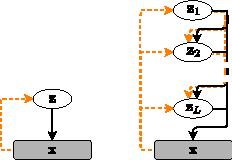
\includegraphics[width=0.5\textwidth]{figs/thesis/vae-vs-hierarchical-vae.pdf}
    \caption{A comparison of the dependency structure of a ``standard'' VAE (left) with that of a top-down hierarchical VAE (right). For each, we show the dependencies of each variable in the encoder's distribution though dashed orange lines and the dependencies of each variable in the prior and decoder's distributions with solid black lines.}
    \label{fig:vae-vs-hierarchical-vae}
\end{figure}
A hierarchical VAE~\citep{gregor2015draw,kingma2016improving,sonderby2016ladder,klushyn2019learning} is a special case of a VAE which has latent variables $\rvz$ with a particular structure. In particular, $\rvz$ is partitioned into $L$ disjoint groups, $\rvz_1,\ldots,\rvz_L$. The prior $p_\theta(\rvz) = p_\theta(\rvz_1,\ldots,\rvz_L)$ and encoder $q(\rvz|\rvx) = q_\phi(\rvz_1,\ldots,\rvz_L|\rvx)$ are then factorised to enable them to represent structured distributions over $\rvz$. Exactly how these distributions are factorised is a design choice but the hierarchical VAEs that we will consider in this thesis are ``top-down'' meaning that they factorise the prior and the encoder distributions in the same order~\citep{vahdat2020nvae,child2020very}:
\begin{equation}
    p_\theta(\rvz) = \prod_{l=1}^L p_\theta(\rvz_l|\rvx,\rvz_{<l}) \quad \text{and} \quad q_\phi(\rvz|\rvx) = \prod_{l=1}^L q_\phi(\rvz_l|\rvx,\rvz_{<l})
\end{equation}
where $\rvz_{<l}$ is the set of all latent variable groups from $\rvz_1$ (inclusive) to $\rvz_{l}$ (exclusive) if $l > 1$ and is null otherwise. We show this dependency structure graphically in \cref{fig:vae-vs-hierarchical-vae}.

Hierarchical VAEs are closely related to diffusion models, and in fact diffusion models can be interpreted as a special case of a hierarchical VAE. Given an increasing sequence of noise standard deviations $\sigma(1),\ldots,\sigma(L)$, we can present a variance-exploding diffusion model as a top-down hierarchical VAE with an encoder
\begin{align}
    q(\rvz|\rvx) &= q(\rvz_1|\rvx) \prod_{l=2}^L q(\rvz_l | \rvx, \rvx_{l-1}) \\
    &= \gN( \rvz_1 ; \rvx, \sigma(L)^2 \mI ) \prod_{l=2}^L \gN( \rvz_l | \mu^l_Q(\rvz_{l-1}, \rvx), {\sigma_Q^l}^2 \mI )
\end{align}
where $\mu^l_Q(\rvz_{l-1}, \rvx) := \mu_Q(\rvz_{l-1}, \rvx; \rho, \sigma)$ and $\sigma^l_Q := \sigma_Q(\rho, \sigma)$ with $\mu_Q$ and $\sigma_Q$ as defined in \cref{eq:mu-q,eq:sigma-q} and $\rho := \sigma(L-l)$, $\sigma := \sigma(L+1-l)$. Note that this encoder has no learnable parameters, i.e. $\phi$ is empty. In the setting described in \cref{sec:diffusion-likelihood}, a diffusion model then approximates each $p_\theta(\rvz_l|\rvz_{<l})$ as a Gaussian. The use of a fixed encoder and Gaussian forms enables many tricks to be used in diffusion models that are not possible for most variational auto-encoders. In particular, diffusion models allow an efficient training objective that can subsample the layer $l$ and compute a loss estimate for a data point using a single value of $l$, whereas a the loss for a hierarchical VAE must typically be summed over all layers for every data point. The diffusion framework also enables weighting of the loss to improve perceptual quality, as we described in \cref{sec:diffusion-perceptual-quality}, and the use of ODEs or SDEs for improved performance at test-time versus explicitly sampling from each $p_\theta(\rvz_l|\rvz_{<l})$.
A major advantage of VAEs, on the other hand, is the learnable encoder which makes it theoretically possible to learn fast and effective procedures for sampling datapoints other than simply progressively removing Gaussian noise. 

Although diffusion models currently dominate at the core tasks of e.g. image and video generation~\citep{esser2024scaling,brooks2024video}, variants of VAEs are used for other purposes including as tools to compress data $\rvx$ into latent variables $\rvz$ that are then modelled with other techniques like diffusion models. We also note that the two-stage diffusion model~\cref{sec:2sdm-2sdm-method} could be interpreted as a form of variational auto-encoder in which the prior $p_\theta(\rvz)$ and decoder $p_\theta(\rvx|\rvz)$ are both parameterised by diffusion models and the encoder is frozen to a pretrained value. We believe that it is valuable to demonstrate that flexible generative modelling works within the variational auto-encoder framework and for these reasons, and to provide more reason to believe that it could apply to other generative modelling frameworks in addition.

\section{A Review of Conditional Variational Auto-Encoders}
\label{sec:conditional-vae}

% \section{Conditional Variational Auto-Encoders}
Our focus in this thesis is on conditional, rather than unconditional, generative models. In the setting we consider we want to approximate the conditional distribution $p_\theta(\rvx|\rvy)$ and at training time have access to either a joint distribution $p_\theta(\rvx,\rvy)$ or a dataset of $(\rvx, \rvy)$ pairs that we can use to approximate the joint distribution.

In order to match the distribution modeled by a VAE to such a conditional distribution, at least one of the prior or decoder should be made conditional on $\rvz$. To cover all cases, we will write both as conditional on $\rvy$. That is, we will denote the prior distribution of a conditional VAE $p_\theta(\rvz|\rvy)$ and the decoder's distribution as $p_\theta(\rvx|\rvy,\rvz)$. The encoder may in principle also be made conditional on $\rvy$, but that is not the case for any of the generative models considered in this thesis and so we will continue to write it as $q_\phi(\rvz|\rvx)$. See \cref{tab:vae_components} for a summary of these differences. The distribution modelled is, as before, obtained by marginalising over $\rvz$ as
\begin{equation} \label{eq:vae-marginal}
p_\theta(\rvx|\rvy) = \int p_\theta(\rvx|\rvy,\rvz)p_\theta(\rvz|\rvy) \mathrm{d}\rvz
\end{equation}
and the training objective for both $\theta$ and $\phi$ is
\begin{equation}
    \gL(\rvx, \rvy, \theta, \phi) = \EX_{q_\phi(\rvz|\rvx)} \left[ \log p_\theta(\rvx|\rvy,\rvz) + \log \frac{p_\theta(\rvz|\rvy)}{q_\phi(\rvz|\rvx)} \right].
\end{equation}

To understand the properties of VAEs, we now take a look at a few ways to decompose this training objective. One is to separate the objective into a reconstruction loss and a KL divergence:
\begin{align}
    \gL(\rvx, \rvy, \theta, \phi) &= \underbrace{\EX_{q_\theta(\rvz|\rvx)} \left[ \log p_\theta(\rvx|\rvz) \right]}_\text{reconstruction loss} + \underbrace{\kl{q_\phi(\rvz|\rvx)}{p_\theta(\rvz)}}_\text{KL divergence},
\label{eq:marginal-is}
\end{align}
The reconstruction loss encourages the encoder and decoder to be learned such that little information is lost if we map a data point $\rvx$ to latent space and back. The KL divergence penalises differences between the encoder's proposal distribution and the prior distribution.

If we consider the expectation of the objective over the data distribution, we can get furhter insight by separating terms into the entropy of the target distribution and a KL divergence:
\begin{align}
  \EX_{\pdata(\rvx,\rvy)} &\left[ \mathcal{L}(\rvx, \rvy, \theta, \phi) \right] \\
  =& \EX_{\pdata(\rvx,\rvy)} \EX_{q_\phi(\rvz|\rvx)} \left[ \log \pdata(\rvx|\rvy) + \log \frac{p_\theta(\rvx,\rvz|\rvy)}{q_\phi(\rvz|\rvx)\pdata(\rvx|\rvy)} \right]\\
    =& -\mathcal{H}\left[ \pdata(\rvx|\rvy) \right] - \kl[\big] { \pdata(\rvx|\rvy) q_\phi(\rvz|\rvx) }{ p_\theta(\rvx,\rvz|\rvy) }. \label{eq:elbo-kl-joints}
\end{align}
where $p_\theta(\rvx,\rvz|\rvy)$ is the joint distribution defined as $p_\theta(\rvx|\rvy,\rvz)p_\theta(\rvz|\rvy)$ and $\mathcal{H}\left[ \pdata(\rvx|\rvy) \right]$ is the differential entropy of the target distribution. While the differential entropy is not guaranteed to be finite in general, it always will be when $\rvx$ is finite, as is common for pixel values in the image and video domains. Since the KL divergence is always non-negative, our training objective is upper-bounded by the differential entropy. Additionally, the KL-divergence is in the direction which causes mass-covering behaviour~\citep{bishop2006pattern} and so we can expect the learned distribution $p_\theta(\rvx|\rvy)$ to assign probability broadly over the data distribution $\pdata(\rvx|\rvy)$, with any missed modes being heavily penalised.

% \begin{table}[t]
% \centering
% % \begin{tabular}{c|c|c|c}
% %  & Prior & Decoder & Encoder \\ 
% % \hline
% % Unconditional VAE & \( p_\theta(\rvz) \) & \( p_\theta(\rvx|\rvz) \) & \( q_\phi(\rvz|\rvx) \) \\
% % Conditional VAE & \( p_\theta(\rvz|\rvy) \) & \( p_\theta(\rvx|\rvy,\rvz) \) & \( q_\phi(\rvz|\rvx) \) \\
% % \end{tabular}
% \begin{tabular}{l|ll|ll}
%  & \multicolumn{2}{c|}{Unconditional} & \multicolumn{2}{c}{Conditional} \\ 
% \cline{2-5}
% & Notation & Definition & Notation & Definition \\ 
% \hline
% Prior & \( p_\theta(\rvz) \) & primitive  & \( p_\theta(\rvz|\rvy) \) & primitive  \\
% Decoder & \( p_\theta(\rvx|\rvz) \) & primitive  & \( p_\theta(\rvx|\rvy,\rvz) \) & primitive \\
% Encoder & \( q_\phi(\rvz|\rvx) \) & primitive  & \( q_\phi(\rvz|\rvx) \) & primitive \\
% Predictive & \( p_\theta(\rvx) \) & \( \int p_\theta(\rvx|\rvz)p_\theta(\rvz) \mathrm{d}\rvz \)  & \( p_\theta(\rvx|\rvy) \) & \( \int p_\theta(\rvx|\rvy,\rvz)p_\theta(\rvz) \mathrm{d}\rvz \) \\
% \end{tabular}
% \caption{Comparison of our notation for distributions relating to an unconditional versus a conditional VAE. The prior, decoder, and encoder distributions are primitives directly parameterised by neural networks. The predictive distribution, which we train to match a target distribution, is defined via a marginalisation.}
% \label{tab:vae_components}
% \end{table}



% \section{Hierarchical Variational Auto-Encoders} \label{sec:hierarchical-vae}
% In this section we introduce the conditional version of a hierarchical VAE, but note that our description can be transferred to the unconditional setting by removing any dependencies on $\rvy$ or setting $\rvy$ to null. A (conditional) hierarchical VAE~\citep{gregor2015draw,kingma2016improving,sonderby2016ladder,klushyn2019learning} is a (conditional) VAE in which the latent variables $\rvz$ have a particular structure. In particular, $\rvz$ is partitioned into $L$ disjoint groups, $\rvz_1,\ldots,\rvz_L$. The prior $p_\theta(\rvz|\rvy) = p_\theta(\rvz_1,\ldots,\rvz_L|\rvy)$ and encoder $q(\rvz|\rvx,\rvy) = q_\phi(\rvz_1,\ldots,\rvz_L|\rvx,\rvy)$ are then factorised to enable them to represent structured distributions over $\rvz$. How these distributions are factorised is a design choice.
% The hierarchical VAEs that we will consider in this thesis are ``top-down'' meaning that they factorise the prior and the encoder distributions in the same order~\citep{vahdat2020nvae,child2020very}:
% \begin{equation}
%     p_\theta(\rvz) = \prod_{l=1}^L p_\theta(\rvz_l|\rvx,\rvz_{<l}) \quad \text{and} \quad q_\phi(\rvz|\rvx) = \prod_{l=1}^L q_\phi(\rvz_l|\rvx,\rvz_{<l})
% \end{equation}
% where $\rvz_{<l}$ is the set of all latent variable groups from $\rvz_1$ (inclusive) to $\rvz_{l}$ (exclusive) if $l > 1$ and is null otherwise. We show this dependency structure graphically in \cref{fig:vae-vs-hierarchical-vae}.

% \begin{figure}
%     \centering
%     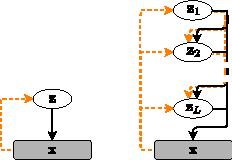
\includegraphics[width=0.5\textwidth]{figs/thesis/vae-vs-hierarchical-vae.pdf}
%     \caption{A comparison of the dependency structure of a ``standard'' VAE (left) with that of a top-down hierarchical VAE (right). For each, we show the dependencies of each variable in the encoder's distribution though dashed orange lines and the dependencies of each variable in the prior and decoder's distributions with solid black lines. Note that, in the case of a conditional VAE, there are additional dependencies of all prior and decoder distributions on $\rvy$, which we do not show.}
%     \label{fig:vae-vs-hierarchical-vae}
% \end{figure}

\clearpage
\chapter{Flexibly-conditional variational auto-encoders}
\label{ch:cigcvae}

% The line of research we look at in this section has two major differences from earlier sections:
% \begin{itemize}
%     \item We look at VAEs instead of diffusion models. Really useful to be able to do arbitrarily-conditional generative modelling with diverse methodologies. And especially if you want to do e.g. latent diffusion this is SOTA. We believe this is the highest-resolution arbitrarily-conditional VAE out there.
%     \item We will look at how to quickly train these systems. Should mention related work including ControlNet that now does similar things with diffusion models
% \end{itemize}

So far in this dissertation we have enabled flexible conditioning in various settings using diffusion models. While diffusion models have demonstrated very good performance on image and video-based tasks, it is not the only modelling methodology with which flexible conditioning is possible. For example, flexible conditioning has already been demonstrated with variational auto-encoders (VAEs)~\citep{ivanov2018variational}; generative adversarial networks~\citep{goodfellow2014generative}; and transformer-based token-prediction architectures~\citep{chang2022maskgit}. 

We believe that enabling and improving flexible conditioning within a diverse set of modelling methodologies is important, not least because the dominant modelling methodology for, e.g., image generation has changed over time. VAEs showed good performance on image generation benchmarks in 2013 after being proposed by \citet{kingma2013auto}. Generative adversarial networks~\citep{goodfellow2014generative} were proposed shortly after, and within a few years were preferred for many image generation tasks~\citep{karras2018style}. Autoregressive methods~\citep{van2016pixel} were proposed shortly after and obtained state-of-the-art likelihoods. Advocacy of diffusion models as a leading method for image generation has been widespread since roughly 2021~\citep{dhariwal2021diffusion}. Since then, MaskGIT~\citep{chang2022maskgit} has gained popularity. Even more recently, methods like rectified flow~\citep{esser2024scaling} and consistency models~\citep{song2023consistency}, which build on the diffusion framework, have been shown to exhibit better sampling speed than true diffusion models while retaining good sample quality. As we saw in \cref{ch:conditional-diffusion}, even using two diffusion models to construct a simple multi-stage generative model (2SDM) can give better sample quality than a pure diffusion model. All this is to say that, while diffusion models are currently a highly-competitive approach for image and video generation tasks, this may not remain the case forever. Furthermore, even now, many approaches use latent diffusion models~\citep{rombach2022high,betker2023improving,brooks2024video} that are a combination of a diffusion model and a VAE. In this chapter we will demonstrate a flexibly-conditional image VAE. While it is not the first flexibly-conditional image VAE~\citep{ivanov2018variational}, it significantly improved on prior work in terms of image quality and resolution and, to the best of our knowledge, these aspects remain unmatched among flexibly-conditional VAEs.


% In this chapter we will demonstrate a flexible variational auto-encoder; that is, a flexible generative model that is based on the variational auto-encoder framework~\citep{kingma2013auto,rezende2014stochastic}. Its good performance shows that flexible generative modelling as a concept is not tied to the diffusion framework and therefore could prove to be future-proof as modelling methodologies change.

\begin{figure*}[t]
  \centering
  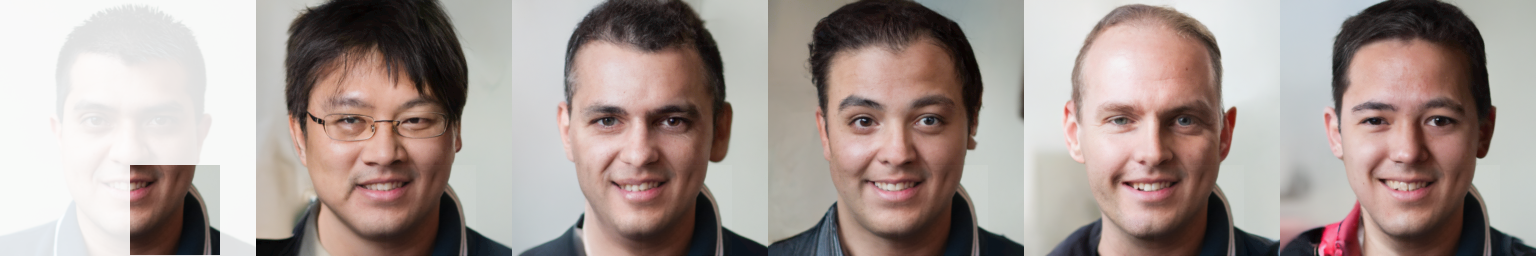
\includegraphics[width=\textwidth]{figs/cigcvae/qual/0_0_patches-4.png}
  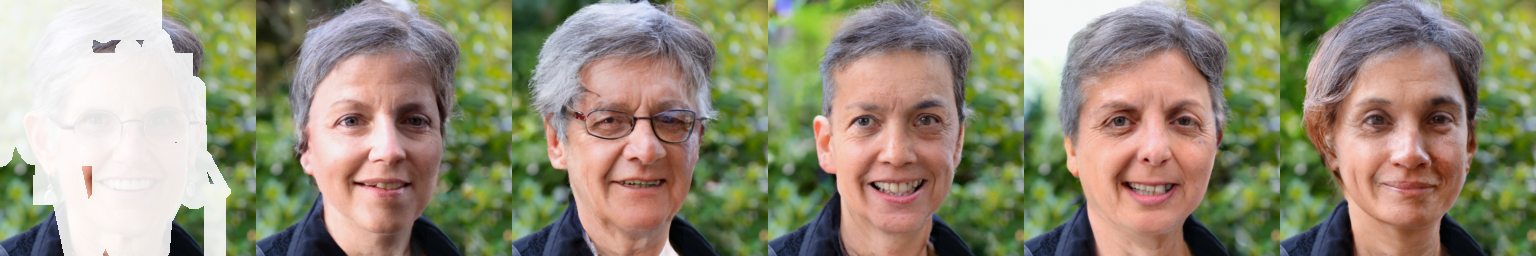
\includegraphics[width=\textwidth]{figs/cigcvae/qual/59_2_3_modddd.png}
  \caption{\textbf{Left column:} Images with most pixels masked out.
    \textbf{Rest:} Completions from IPA, our proposed method.
  }
  \label{fig:cigcvae-headline}
\end{figure*}

% We will demonstrate flexibly-conditional VAEs primarily on the image inpainting problem. 
In particular, we train a single model which is capable of generating an image conditioned on any subset of that image's pixel values, and so is capable of image inpainting. We demonstrate that such a model can achieve excellent performance; see results in \cref{fig:cigcvae-headline}. Furthermore, to mitigate the slow and expensive training usually associated with VAEs, we demonstrate that a flexibly-conditional VAE can be trained with little computational cost by initialising training with a pretrained unconditional VAE. 

% We belive that this finding is extremely encouraging in terms of the applicability of flexible generative modelling; it suggests that the learned representations that are useful for flexible generation are similar to those that are good for unconditional generation, at least within the VAE framework. This provides evidence that flexible generative modelling and unconditional generative modelling are tightly-related tasks, giving us hope that other model classes that are good at unconditional generation will also be amenable to flexibly conditional generation.


Before introducing flexibly-conditional VAEs, we will review background material on VAEs in \cref{sec:vae}. We will then motivate and explain our proposed method for training flexibly-conditional VAEs in \cref{sec:ipa}; report experimental results in \cref{sec:cigcvae-experiments}; and describe a hypothetical application of an inpainting model with the capabilities ours exhibits in \cref{sec:cigcvae-boed}.


\section{A review of variational auto-encoders}
\label{sec:vae}
As with our review of diffusion models in \cref{ch:diffusion}, we will start by describing VAEs~\citep{kingma2013auto,rezende2014stochastic} as unconditional generative models. We will then explain a conditional variant in \cref{sec:conditional-vae}. Like a diffusion model, a VAE is trained to approximate a data distribution $\pdata(\rvx)$ using samples from that data distribution. Given a VAE with parameters $\theta$, we will denote the distribution over data it parameterises $p_\theta(\rvx)$. The key feature of a VAE is that it breaks the process of generating data into two steps: in the first step a VAE samples a latent variable $\rvz$ from a ``prior'' distribution $p_\theta(\rvz)$. The prior distribution can be fixed, e.g. a unit Gaussian, or can have learnable parameters that are included in $\theta$. In the second step, the VAE parameterises a ``likelihood'' $p_\theta(\rvx|\rvz)$. This can be, e.g., a Gaussian for continuous data~\citep{kingma2013auto} or a categorical for discrete data~\citep{child2020very}, with parameters output in either case by a neural network as a function of $\rvz$. We can therefore write the parameterised distribution $p_\theta(\rvx)$ as the marginal of $p_\theta(\rvx|\rvz)$ over the latent variable $\rvz$,
\begin{equation} \label{eq:vae-marginal}
p_\theta(\rvx) = \int p_\theta(\rvx|\rvz)p_\theta(\rvz) \mathrm{d}\rvz.
\end{equation}
Even if both the prior $p_\theta(\rvz)$ and likelihood $p_\theta(\rvx|\rvz)$ are simple distributions, the marginal $p_\theta(\rvx)$ can be complex since the parameters of the likelihood can be given by arbitrarily complex functions of $\rvz$.

As we discussed for diffusion models in \cref{ch:diffusion}, an ideal training objective would maximise the data likelihood $p_\theta(\rvx)$ averaged over all training examples since this corresponds to a maximum-likelihood estimate of the parameters given the dataset. The required marginalisation in \cref{eq:vae-marginal}, however, means that directly estimating the data likelihood is intractable. Therefore, as for diffusion models, we instead derive a training objective that lower-bounds the data likelihood. Starting by taking an expectation of the log of the data likelihood in \cref{eq:vae-marginal}, we can obtain a lower-bound using a proposal distribution $q_\phi(\rvz|\rvx)$ which can be parameterised by a neural network with parameters $\phi$: % our objective can be converted to the log of an expectation over $q_\phi(\rvz)$:
\begin{align}
    \EX_{\pdata(\rvx)} \left[ \log p_\theta(\rvx) \right] &= \EX_{\pdata(\rvx)} \left[ \log \int p_\theta(\rvx|\rvz)p_\theta(\rvz) \mathrm{d}\rvz \right] \\
    &= \EX_{\pdata(\rvx)} \left[ \log \int p_\theta(\rvx|\rvz) \frac{p_\theta(\rvz)}{q_\phi(\rvz|\rvx)} q_\phi(\rvz|\rvx) \mathrm{d}\rvz \right] \\
    &= \EX_{\pdata(\rvx)} \left[ \log \EX_{q_\phi(\rvz|\rvx)} \left[ p_\theta(\rvx|\rvz) \frac{p_\theta(\rvz)}{q_\phi(\rvz|\rvx)} \right] \right]. \label{eq:vae-marginal-is}
\end{align}
Ideally we would be able to obtain an unbiased estimate of this objective. Due to the logarithm operator outside an intractable expectation this is not feasible but, using Jensen's inequality, we can obtain a training objective that lower bounds it by switching their order: 
\begin{align}
    \gO_\text{VAE}(\theta, \phi) := \EX_{\pdata(\rvx)q_\phi(\rvz|\rvx)} \left[ \log p_\theta(\rvx|\rvz) + \log \frac{p_\theta(\rvz)}{q_\phi(\rvz|\rvx)} \right] \leq \EX_{\pdata(\rvx)} \left[ \log p_\theta(\rvx) \right].
    \label{eq:vae-objective}
\end{align}
Note that we are now describing training as maximising an objective rather than minimising a loss as in earlier chapters. We could, alternatively and equivalently, minimise $\gL_\text{VAE}(\theta, \phi) = -\gO_\text{VAE}(\theta, \phi)$ but we make make this choice to fit a common convention in the VAE literature~\citep{kingma2013auto,sohn2015learning,child2020very,vahdat2020nvae}. The lower-bound in \cref{eq:vae-objective} can be stochastically estimated by sampling data $\rvx$ and then sampling $\rvz$ from $q_\phi(\rvz|\rvx)$ and evaluating the terms inside the expectation with that $\rvz$. Since $q_\phi(\rvz|\rvx)$ ``encodes'' data $\rvx$ into latent variables $\rvz$ we will from now on refer to it as the encoder. The tightness of this lower-bound is strongly dependent on how ``good'' the encoder $q_\phi(\rvz|\rvx)$ is, as we can make clear by rewriting \cref{eq:vae-objective} as
\begin{equation}
    \gO_\text{VAE}(\theta, \phi) := \EX_{\pdata(\rvx)} \left[ \log p_\theta(\rvx) - \kl{q_\phi(\rvz|\rvx)}{p_\theta(\rvz|\rvx)} \right].
\end{equation}
This formulation reveals that the lower-bound is tight if and only if the proposal $q_\phi(\rvz|\rvx)$ is equal to the generally intractable posterior $p_\theta(\rvz|\rvx)$ for all $\rvx$, causing the KL divergence term to be zero. Fortunately, maximising this objective with respect to $\theta$ and $\phi$ will optimise the proposal parameters $\phi$ to better match the intractable posterior as well as optimising $\theta$ to increase the model likelihood, and so it is possible to train both $\theta$ and $\phi$ with a unified objective. The full optimisation problem is therefore to find
\begin{align}
    \argmax_{\theta,\phi} \gO_\text{VAE}(\theta, \phi).
\end{align}

\subsection{Hierarchical variational auto-encoders}
\label{sec:hierarchical-vae}
\begin{figure}
    \centering
    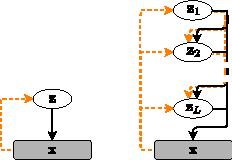
\includegraphics[width=0.5\textwidth]{figs/thesis/vae-vs-hierarchical-vae.pdf}
    \caption{A comparison of the dependency structure of a ``standard'' VAE (left) with that of a top-down hierarchical VAE (right). For each, we show the dependencies of each variable in the encoder's distribution though dashed orange lines and the dependencies of each variable in the prior and decoder's distributions with solid black lines.}
    \label{fig:vae-vs-hierarchical-vae}
\end{figure}
A hierarchical VAE~\citep{gregor2015draw,kingma2016improving,sonderby2016ladder,klushyn2019learning} is a special case of a VAE in which the latent variables $\rvz$ are structured. In particular, $\rvz$ is partitioned into $L$ disjoint groups, $\rvz_1,\ldots,\rvz_L$. The prior $p_\theta(\rvz) = p_\theta(\rvz_1,\ldots,\rvz_L)$ and encoder $q_\phi(\rvz|\rvx) = q_\phi(\rvz_1,\ldots,\rvz_L|\rvx)$ are then factorised to enable them to represent structured distributions over $\rvz$. Exactly how these distributions are factorised is a design choice but the hierarchical VAEs that we will consider in this thesis are ``top-down'' meaning that they factorise the prior and the encoder distributions in the same order~\citep{vahdat2020nvae,child2020very}:
\begin{equation} \label{eq:hierarchical-vae-factorisations}
    p_\theta(\rvz) = \prod_{l=1}^L p_\theta(\rvz_l|\rvx,\rvz_{<l}) \quad \text{and} \quad q_\phi(\rvz|\rvx) = \prod_{l=1}^L q_\phi(\rvz_l|\rvx,\rvz_{<l})
\end{equation}
where $\rvz_{<l}$ is the set of all latent variable groups from $\rvz_1$ (inclusive) to $\rvz_{l}$ (exclusive) if $l > 1$ and is null otherwise. We show this dependency structure graphically in \cref{fig:vae-vs-hierarchical-vae}.

\subsection{Relationship to diffusion models}
Hierarchical VAEs are closely related to diffusion models, and in fact diffusion models can be interpreted as a special case of a hierarchical VAE. Given an increasing sequence of noise standard deviations $\Sigma[1],\ldots,\Sigma[L]$, we can present a variance-exploding diffusion model as a bottom-up hierarchical VAE with a simple encoder which progressively adds Gaussian noise to transition between each layer of latent variables:
\begin{align}
    q(\rvz|\rvx) &= q(\rvz_L|\rvx) \prod_{l=2}^L q(\rvz_{l-1} | \rvz_{l}) \\
    % &= \gN( \rvz_L ; \rvx, \Sigma[1]^2 \mI ) \prod_{l=L}^2 \gN( \rvz_{l-1} ; \rvz_{l}, (\Sigma[l]^2-\Sigma[l-1]^2) \mI ) \\
    &= \gN( \rvx_1 ; \rvx, \Sigma[1]^2 \mI ) \prod_{l=2}^L \gN( \rvx_{l} ; \rvx_{l-1}, (\Sigma[l]^2-\Sigma[l-1]^2) \mI )
\end{align}
where, to allow for easier comparisons to \cref{ch:diffusion}, we have defined $\rvx_1 := \rvz_L$, $\rvx_2 := \rvz_{L-1}$, \ldots, $\rvx_L := \rvz_1$. Due to the conjugacy of Gaussians, we can equivalently present a factorisation of $q(\rvz|\rvx)$ as a top-down hierarchical VAE encoder. This is reminiscent of the factorisation of $q$ used to derive a lower-bound on the diffusion model likelihood in \cref{sec:diffusion-likelihood}:
\begin{align}
    q(\rvz|\rvx) &= q(\rvz_1|\rvx) \prod_{l=2}^L q(\rvz_l | \rvx, \rvz_{l-1}) \\
    % &= \gN( \rvz_1 ; \rvx, \Sigma[L]^2 \mI ) \prod_{l=2}^L \gN( \rvz_l ; \mu^l_Q(\rvz_{l-1}, \rvx), {\sigma_Q^l}^2 \mI ) \\
    &= \gN( \rvx_L ; \rvx, \Sigma[L]^2 \mI ) \prod_{l=2}^L \gN( \rvx_{l-1} ; \mu^l_Q(\rvx_{l}, \rvx), {\sigma_Q^l}^2 \mI )
\end{align}
where $\mu^l_Q(\rvz_{l}, \rvx) := \mu_Q(\rvz_{l}, \rvx; \rho, \sigma)$ and $\sigma^l_Q := \sigma_Q(\rho, \sigma)$ with $\mu_Q$ and $\sigma_Q$ as defined in \cref{eq:mu-q,eq:sigma-q} and $\rho := \Sigma[l-1]$, $\sigma := \Sigma[l]$. Note that this encoder has no learnable parameters, i.e. $\phi$ is empty. In the DDPM style of sampling described in \cref{sec:diffusion-likelihood}, a diffusion model approximates each $p_\theta(\rvz_l|\rvz_{<l})$ as a Gaussian.

A diffusion model's implicit use of this fixed encoder with this simple Gaussian form
enables some improvements to diffusion model training that are not possible for most VAEs. In particular, diffusion models allow an efficient training objective that can sample a single layer $l$ (i.e. diffusion timestep $t$) and efficiently compute a loss estimate for a data point using this single value of $l$ (or $t$). In contrast, the loss for a hierarchical VAE must typically be computed by evaluating all layers for each data point. The diffusion framework also enables weighting of the loss to improve perceptual quality, as we described in \cref{sec:diffusion-perceptual-quality}, and the use of ODEs or SDEs for improved performance at test-time versus explicitly sampling from each $p_\theta(\rvz_l|\rvz_{<l})$.

Advantages of the VAE framework, on the other hand, include the learnable encoder which makes it theoretically possible to learn fast and effective procedures for sampling datapoints other than the gradual removal of Gaussian noise. VAEs can also be designed to yield latent variables with particular properties, so even a VAE which has gives poor sample quality when used for unconditional generation may be useful as part of, e.g., a latent diffusion model~\citep{rombach2022high,brooks2024video}.

% Although diffusion models currently outperform state-of-the-art VAEs at image and video generation~\citep{esser2024scaling,brooks2024video}, variants of VAEs are still a tool used in state-of-the-art workflows such as latent diffusion models~\citep{rombach2022high,brooks2024video}. In these settings, VAEs can be used to compress data $\rvx$ into lower-dimensional latent variables $\rvz$ that are then modelled with other techniques like diffusion models~\citep{rombach2022high}. Taking a broader perspective, the two-stage diffusion model from \cref{sec:2sdm-2sdm-method} could also be interpreted as a form of variational auto-encoder in which the prior $p_\theta(\rvz)$ and decoder $p_\theta(\rvx|\rvz)$ are both parameterised by diffusion models and the encoder $q_\phi(\rvz|\rvx)$ is frozen to be a Dirac distribution on the CLIP image embedding of $\rvx$. 


\subsection{Conditional variational auto-encoders}
\label{sec:conditional-vae}
We now transport the VAE framework described above into the conditional generative modelling setting, where we want to train an approximation of the posterior $\pdata(\rvx|\rvy)$ given a dataset of $(\rvx, \rvy)$ pairs sampled from $\pdata(\cdot,\cdot)$.

Recall that the distribution over data $\rvx$ modelled by a VAE is defined through a combination of its prior and its decoder, as described in \cref{eq:vae-marginal}. For this distribution to depend on $\rvy$, as it must in a conditional VAE, at least one of the prior or decoder must take $\rvy$ as input. In the conditional VAEs considered in this thesis, only the prior will depend on $\rvy$. For conditional VAEs we will therefore write the prior as $p_\theta(\rvz|\rvy)$ while continuing to write the decoder as $p_\theta(\rvx|\rvz)$. In the case of a hierarchical VAE, we will allow for all layers to be conditioned on $\rvy$ and so factorise $p_\theta(\rvz|\rvy)$ as
\begin{equation}
    p_\theta(\rvz|\rvy) = \prod_{l=1}^L p_\theta(\rvz_l|\rvy,\rvz_{<l})
\end{equation}
The encoder can optionally also take $\rvy$ as an input~\citep{sohn2015learning}, but it will not in the VAEs presented in this thesis so we will continue writing it as simply $q_\phi(\rvz|\rvx)$. In the hierarchical case we will again factorise it as
\begin{equation} \label{eq:conditional-hierarchical-vae-factorisations}
    q_\phi(\rvz|\rvx) = \prod_{l=1}^L q_\phi(\rvz_l|\rvx,\rvz_{<l})
\end{equation}
as in \cref{eq:hierarchical-vae-factorisations}.

The distribution over data modelled by the VAE now becomes
\begin{equation} \label{eq:conditional-vae-marginal}
p_\theta(\rvx|\rvy) = \int p_\theta(\rvx|\rvz)p_\theta(\rvz|\rvy) \mathrm{d}\rvz.
\end{equation}
and we can derive a training objective similar to \cref{eq:vae-objective} as a lower-bound on $\log p_\theta(\rvx|\rvy)$, averaged over $(\rvx, \rvy)$ pairs from the training distribution:
\begin{align}
    \EX_{\pdata(\rvx, \rvy)} \left[ \log p_\theta(\rvx|\rvy) \right] &= \EX_{\pdata(\rvx, \rvy)} \left[ \log \int p_\theta(\rvx|\rvz)p_\theta(\rvz|\rvy) \mathrm{d}\rvz \right] \\
    &= \EX_{\pdata(\rvx, \rvy)} \left[ \log \int p_\theta(\rvx|\rvz)\frac{p_\theta(\rvz|\rvy)}{q_\phi(\rvz|\rvx)}q_\phi(\rvz|\rvx) \mathrm{d}\rvz \right] \\
    &= \EX_{\pdata(\rvx, \rvy)} \left[ \log \EX_{q_\phi(\rvz|\rvx)} \left[ p_\theta(\rvx|\rvz)\frac{p_\theta(\rvz|\rvy)}{q_\phi(\rvz|\rvx)} \right] \right] \\
    &\geq \EX_{\pdata(\rvx, \rvy)} \left[ \EX_{q_\phi(\rvz|\rvx)} \left[ \log p_\theta(\rvx|\rvz) + \log \frac{p_\theta(\rvz|\rvy)}{q_\phi(\rvz|\rvx)} \right] \right] \\
    &:= \gO_\text{CVAE}(\theta, \phi).
\end{align}




Similarly to the unconditional VAE training objective, we can break this down as
\begin{align} \label{eq:conditional-vae-objective}
    \gO_\text{CVAE}(\theta, \phi) = \EX_{\pdata(\rvx,\rvy)} \left[ \underbrace{\EX_{q_\phi(\rvz|\rvx)}\left[\log p_\theta(\rvx|\rvz) \right]}_\text{reconstruction objective} - \underbrace{\kl{q_\phi(\rvz|\rvx)}{p_\theta(\rvz|\rvy)}}_\text{KL divergence} \right]
\end{align}
showing that training the conditional VAE involves balancing maximising a ``reconstruction'' term with minimising an expected KL divergence between the encoder's distribution $q_\phi(\rvz|\rvx)$ and the conditional prior $p_\theta(\rvz|\rvy)$.

We now consider one further decomposition of $\gO_\text{CVAE}(\theta, \phi)$ which yields additional insights about the properties of conditional VAEs:
\begin{align}
    \gO_\text{CVAE}(\theta, \phi) =& \EX_{\pdata(\rvx,\rvy)q_\phi(\rvz|\rvx)} \left[ \log \frac{\log p_\theta(\rvx|\rvz)p_\theta(\rvz|\rvy)}{q_\phi(\rvz|\rvx)} \right] \\
    =& \EX_{\pdata(\rvx,\rvy)q_\phi(\rvz|\rvx)} \left[ \log \pdata(\rvx|\rvy) + \log \frac{\log p_\theta(\rvx|\rvz)p_\theta(\rvz|\rvy)}{q_\phi(\rvz|\rvx)\pdata(\rvx|\rvy)} \right] \\
    \label{eq:elbo-kl-joints}
    =& \EX_{\pdata(\rvx,\rvy)} \left[ \log \pdata(\rvx|\rvy) \right] \\
    &- \EX_{\pdata(\rvy)} \left[ \kl{q_\phi(\rvz|\rvx)\pdata(\rvx|\rvy)}{p_\theta(\rvx|\rvz)p_\theta(\rvz|\rvy)} \right] \nonumber .
\end{align}
\Cref{eq:elbo-kl-joints} states that the conditional VAE objective is the average likelihood of $\rvx$ given $\rvy$ under the data distribution minus a KL divergence describing the match between the model's distribution $p_\theta(\rvx|\rvz)p_\theta(\rvz)$ and a distribution given by encoding sampled data $q_\phi(\rvz|\rvx)\pdata(\rvx|\rvy)$. Given that asymmetry of the KL divergence~\citep{bishop2006pattern}, it also reveals that the learned $p_\theta(\rvx|\rvz)p_\theta(\rvz)$ will be mass-covering and so can be expected to produce more diverse samples than are realistic if it is unable to perfectly match $q_\phi(\rvz|\rvx)\pdata(\rvx|\rvy)$. Any modes of the true conditional distribution that the model's distribution misses will be heavily penalised by $\gO_\text{CVAE}(\theta,\phi)$. 

We end with a note on how the conditional VAE objective (\cref{eq:conditional-vae-objective}) can be estimated in practice. The reconstruction term in \cref{eq:conditional-vae-objective} is tractable to estimate for each $(\rvx,\rvy)$ with a single sample of $\rvz$ as long as likelihoods can be computed under $p_\theta(\rvx|\rvz)$. The KL divergence in \cref{eq:conditional-vae-objective} will be tractable in  a traditional (non-hierarchical) VAE where the distributions compared are e.g. both Gaussian. In a hierarchical VAE it is generally not tractable but it is possible to obtain the following unbiased estimate of it. In particular, in a top-down hierarchical VAE~\citep{vahdat2020nvae,child2020very} we can decompose it as
\begin{align}
    \kl{q_\phi(\rvz|\rvx)}{p_\theta(\rvz|\rvy)} &= \EX_{q_\phi(\rvz|\rvx)} \left[  \log \frac{q_\phi(\rvz|\rvx)}{p(\rvz|\rvy)} \right] \\
    &= \EX_{q_\phi(\rvz|\rvx)} \left[ \log \frac{\prod_{l=1}^L q_\phi(\rvz_l|\rvx,\rvz_{<l})}{\prod_{l=1}^L p_\theta(\rvz_l|\rvy,\rvz_{<l})} \right] \\
    &= \EX_{q_\phi(\rvz|\rvx)} \left[ \sum_{l=1}^L \log \frac{q_\phi(\rvz_l|\rvx,\rvz_{<l})}{p_\theta(\rvz_l|\rvy,\rvz_{<l})} \right] \\
    &= \EX_{q_\phi(\rvz|\rvx)} \left[ \sum_{l=1}^L \kl{q_\phi(\rvz_l|\rvx,\rvz_{<l})}{p_\theta(\rvz_l|\rvy,\rvz_{<l})} \right]
\end{align}
which is an expectation of the sum of layer-wise KL divergences. Each layer-wise KL divergence is tractable under common parameterisations of $p_\theta(\rvz_l|\rvy,\rvz_{<l})$ and $q_\phi(\rvz_l|\rvx,\rvz_{<l})$ like Gaussian distributions. We can therefore estimate the overall KL divergence by simply drawing one sample of $\rvz$ from the encoder and using it to compute layer-wise KL divergences.


\begin{figure*}[t]
  \centering
  \begin{subfigure}[b]{.32\textwidth}
    \centering
    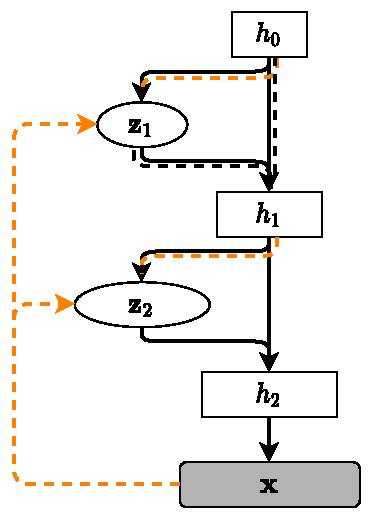
\includegraphics[height=3.8cm]{figs/cigcvae/arch_small-standard.pdf}
    \caption{Estimating ELBO.}
    \label{fig:cigcvae-hierarchical-vae}
  \end{subfigure}
  \begin{subfigure}[b]{.32\textwidth}
    \centering
    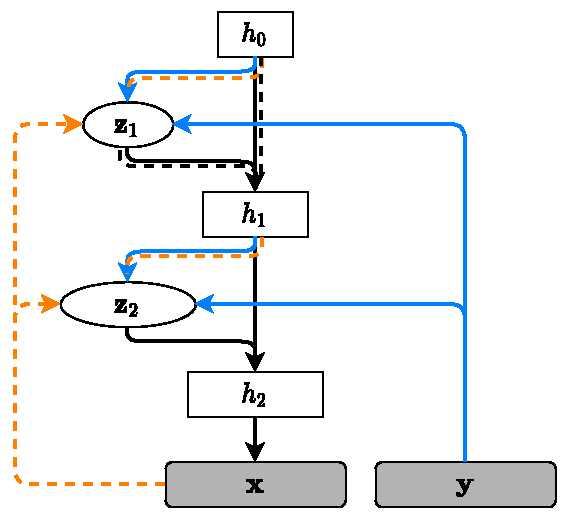
\includegraphics[height=3.8cm]{figs/cigcvae/arch_small-forward.pdf}
    \caption{Estimating $\gO_\text{CVAE}$.}
    \label{fig:cigcvae-forward-arch}
  \end{subfigure}
  \begin{subfigure}[b]{.32\textwidth}
    \centering
    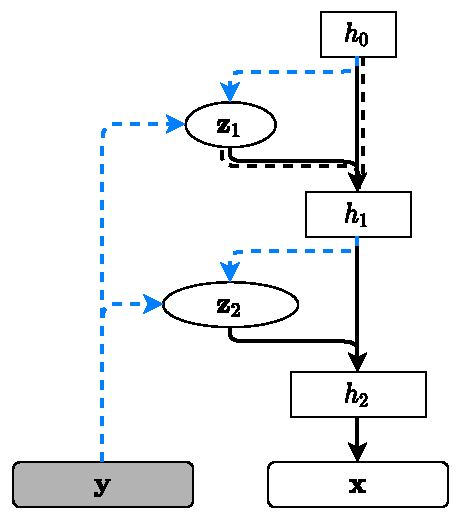
\includegraphics[height=3.8cm]{figs/cigcvae/arch_small-sampling.pdf}
    \caption{Sampling $\rvx\sim p_{\theta,\psi}(\cdot|\rvy)$.}
    \label{fig:cigcvae-reverse-arch}
  \end{subfigure}
  \vspace{-1mm}
  \caption{A hierarchical VAE architecture with $L=2$ layers of latent
    variables. Part (a) illustrates the computation of the ELBO for an
    unconditional VAE; part (b) illustrates the computation of our training
    objective $\gO_\text{CVAE}$; and part (c) illustrates the drawing
    of conditional samples. The encoder is shown in orange; the prior and the
    decoder (which maintains a deterministic hidden state $h_{l}$) are both
    shown in black; and the conditional prior is shown in blue. The computation
    graph needed to sample $\rvz$ in each case is drawn with dashed lines, and
    the remainder of the computation graph is drawn with solid lines.}
  \label{fig:cigcvae-conditional-architectures}
  \vspace{-2mm}
\end{figure*}


\section{Inference in a pretrained auto-encoder}
\label{sec:ipa}

We now describe our approach to training conditional, and flexibly-conditional, VAEs. It is designed to allow initialisation from a pretrained unconditional VAE, enabling fast and cheap training.  This is particularly important in the VAE setting because of the typically slow training times seen with VAEs. Take as an example the VD-VAE~\citep{child2020very}, which we will build on in this chapter. The VD-VAE takes on the order of 1 GPU-year to train on the $256\times256$ FFHQ dataset~\citep{karras2019style} whereas the generative adversarial networks (GANs) that were state-of-the-art at the time of VD-VAE's publication could be trained on the same
dataset in a matter of GPU-weeks~\citep{lin2021anycost,karras2020analyzing}. One hypothesis for the cause of this disparity
is that, whereas the ``mass-covering'' training objective for a VAE forces it to
assign probability mass over the entirety of the data distribution, a GAN can
``cut corners'' by dropping modes~\citep{arora2017gans,arora2017generalization}. Conditional GANs~\citep{zheng2019pluralistic,zhao2021large} and conditional VAEs~\citep{sohn2015learning,ivanov2018variational} suffer from the same disparity in training times as their unconditional counterparts. We will show that re-using publicly available pretrained models to initialise our conditional VAEs can lead to training times and sample quality competitive with GAN-based approaches while avoiding mode dropping.

% We present an approach based on the conditional VAE framework but, to mitigate the associated slow training times, we design the architecture so that we can incorporate pretrained unconditional VAEs. 


While requiring an existing pretrained model is a limitation, we note that:
\textbf{(1)} The unconditional VAE need not have been (pre-)trained on the same dataset as the conditional model; we show unconditional models trained on
ImageNet are suitable for later use with various photo datasets.
\textbf{(2)} A single unconditional VAE can be used for later training of
conditional VAEs on any desired conditional generation tasks (e.g.~the same
image model may be later used for image inpainting or image colourisation).
\textbf{(3)} There is an increasing trend in the machine learning community towards
sharing large, expensively trained models~\citep{wolf2020transformers},
sometimes referred to as foundation models~\citep{bommasani2021opportunities}.
Most of the unconditional VAEs in our experiments use publicly-available
pretrained weights released by \citet{child2020very}. By presenting a use case
for foundation models in image modelling, we hope to encourage even more sharing
of pretrained weights in this domain.

We demonstrate our approach in several settings but our focus is image inpainting, the problem of inferring the posterior distribution over images given the observation of a subset of pixel values. For some applications such as photo-editing the implicit distribution defined by GANs is good enough. We argue that our approach has substantial advantages when
image inpainting is used as part of a larger pipeline, and discuss one possible
instance of this in \cref{sec:cigcvae-boed}: Bayesian optimal experimental design (BOED)
for guiding a sensor or hard attention
mechanism~\citep{ma2018eddi,harvey2019near,rangrej2021achieving}. In this case,
missing modes of the posterior over images is likely to lead to bad decisions.
We show that our objective corresponds to the mass-covering KL divergence and so
covers the posterior well. This is supported empirically by results indicating that, not only is the visual quality of our inpaintings (see \cref{fig:cigcvae-headline}) close to the
state-of-the-art~\citep{zhao2021large}, but our coverage of the ``true''
posterior over inpaintings is superior to that of any of our baselines.


\subsection{Notation}
We have described VAE parameters as a combination of $\phi$, the encoder parameters, and $\theta$, parameters shared between the prior and decoder. In the conditional case, we modify $\theta$ to contain the conditional prior parameters and decoder parameters. In the following sections we will want to simultaneously consider decoder parameters, unconditional prior parameters, and conditional prior parameters. To do so, we will from now on use $\theta$ to mean the unconditional prior and decoder parameters, as for an unconditional VAE. We will then denote the conditional prior parameters $\psi \in \Psi$.
% To convert an unconditional VAE architecture to a conditional architecture, we
% introduce a \textit{conditional prior} with parameters $\psi\in\Psi$.
% Given a conditioning input $\rvy$ (which could be, e.g., an image with some
% pixels masked out in the case of inpainting),
To denote the conditional prior's approximate posterior over the latent variables given conditioning information we therefore use $p_\psi(\rvz|\rvy)$.
%
Our approximation of $\pdata(\rvx|\rvy)$ becomes
\begin{equation}
  \label{eq:marginal-image-posterior}
  p_{\theta,\psi}(\rvx|\rvy) := \int p_\theta(\rvx|\rvz)p_\psi(\rvz|\rvy) \mathrm{d}\rvz
\end{equation}
with learnable parameters $\theta$ and $\psi$. We can sample from
$p_{\theta,\psi}(\rvx|\rvy)$ by sampling $\rvz\sim p_\psi(\cdot|\rvy)$ and then
$\rvx\sim p_\theta(\cdot|\rvz)$ as illustrated in \cref{fig:cigcvae-reverse-arch}. 
%

We introduce some more notation before describing our method further. Let the
distribution of paired data be $\pdata(\rvx, \rvy)$, and recall that
training an unconditional VAE matches two joint distributions: the distribution
of unconditional samples, $p_\theta(\rvz, \rvx)$; and the distribution
resulting from sampling data $\rvx$ and then encoding it, $\pdata(\rvx)q(\rvz|\rvx)$. We define extensions of each to include $\rvy$:
\begin{align}
  p_\theta(\rvz, \rvx, \rvy) &= p_\theta(\rvz)p_\theta(\rvx|\rvz)\pdata(\rvy|\rvx), \label{eq:pmodel} \\
  q_\phi(\rvz, \rvx, \rvy) &= \pdata(\rvx, \rvy)q_\phi(\rvz|\rvx), \label{eq:r}
\end{align}
% alternatively:
% \begin{align}
%   p_\theta(\rvz, \rvx, \rvy) &= p_\theta(\rvz)p_\theta(\rvx|\rvz)\pdata(\rvy|\rvx), \label{eq:pmodel} \\
%   q_\phi(\rvz, \rvx, \rvy) &= \pdata(\rvx, \rvy)q_\phi(\rvz|\rvx), \label{eq:r}
% \end{align}
where $\pdata(\rvy|\rvx)$ is a (potentially intractable) conditional
distribution of $\pdata(\rvx, \rvy)$.
%
Note that $p_\theta(\rvz, \rvx, \rvy)$ and $q_\phi(\rvz, \rvx, \rvy)$ are exactly the two distributions matched by the conditional VAE
objective in \cref{eq:elbo-kl-joints}, $p_\theta(\rvz)p_\theta(\rvx|\rvz)$ and $\pdata(\rvx)q_\phi(\rvz|\rvx)$, with an additional factor of
$\pdata(\rvy|\rvx)$ applied to each.
%
Therefore, if the unconditional VAE represented by $\theta$ and $\phi$ is well
trained, $p_\theta(\rvz, \rvx, \rvy)$ and
$q_\phi(\rvz, \rvx, \rvy)$ will be close. From now on, we will use
$p_\theta$ and $q_\phi$ respectively to refer to any marginals and conditionals of these
joint distributions, with the specific marginal or conditional clear from
context.

So far we have introduced the notation we will use for conditional VAEs. For flexibly-conditional VAEs, we will use exactly the same notation. This means that we will no longer explicitly discuss $\gY$, the list of the observed data indices. Instead, we will define $\rvy$ to implicitly contain $\gY$ in the flexible conditioning setting. In particular, for our flexibly-conditional image models, $\rvy$ will be structured to include a binary mask describing which pixels are observed.

\subsection{Training objective}

Our training objective, previously used for training conditional
VAEs~\citep{sohn2015learning,ivanov2018variational} and neural
processes~\citep{garnelo2018neural}, is
\begin{align}
  \label{eq:forward-elbo}
  \gO_\text{CVAE}(\theta, \phi, \psi) &= \EX_{\pdata(\rvx, \rvy)} \EX_{q_\phi(\rvz|\rvx)} \left[ \log \frac{p_\theta(\tildeI|\rvz)p_\psi(\rvz|\rvy)}{q_\phi(\rvz|\rvx)} \right] \\
  &\leq \EX_{\pdata(\rvx, \rvy)} \left[ \log p_{\theta,\psi}(\tildeI{}|\rvy) \right]
\end{align}
where $\tilde{\rvx}$ is the part of $\rvx$ we wish to predict. In general we can
set $\tildeI{}:=\rvx$ but for inpainting define $\tildeI{}$ to consist of only
the dimensions of $\rvx$ not observed in $\rvy$, abusing notation by
ignoring the implication that $\tildeI{}$ is formally a function of $\rvy$
as well as $\rvx$. Our architectures have pixel-wise independent
likelihoods so $p_\theta(\tildeI{}|\rvz)$ is tractable in either case. \Cref{eq:forward-elbo}
lower-bounds $\log p_{\theta,\psi}(\tildeI{}|\rvy) $ similarly to how the ELBO of
an unconditional VAE lower-bounds $\log p_\theta(\rvx)$. The major difference
is that the prior, $p_\theta(\rvz)$, is replaced by $p_\psi(\rvz|\rvy)$.
This is reflected in \cref{fig:cigcvae-forward-arch} where each $\rvz_l$ is conditioned
on $\rvy$ via the conditional prior.
%
As described in \cref{sec:conditional-vae},
reduced-variance estimates of \cref{eq:forward-elbo} can be obtained by
computing KL divergences between $q(\rvz_l|\rvz_{<l},\rvx)$ and
$p_\psi(\rvz_l|\rvz_{<l},\rvy)$ analytically for each layer $l$..

We are particularly interested in the properties of the learned conditional prior.
Recall the joint distribution $q_\phi(\rvz, \rvx, \rvy) = \pdata(\rvx,
\rvy)q_\phi(\rvz|\rvx)$. Then $q_\phi(\rvz|\rvy)$ is the intractable
posterior given by marginalising out $\rvx$ and conditioning on $\rvy$. We
find that fitting $\psi$ to maximise $\gO_\text{CVAE}(\theta,
\phi, \psi)$ is equivalent to minimising the mass-covering KL divergence
from $q_\phi(\rvz|\rvy)$ to $p_\psi(\rvz|\rvy)$. We formalise
this statement in the following theorem, which is proven in
\cref{proof:forward-kl}.
\begin{theorem} \label{theorem:forward-kl} For any set $\Psi$ of
  permissible values of $\psi$, and for any $\theta\in\Theta$ and
  $\phi\in\Phi$,
  \begin{equation} \label{eq:forward-theorem}
    \argmax_{\psi \in \Psi} \gO_\text{CVAE}(\theta, \phi, \psi) = \argmin_{\psi \in \Psi} \EX_{\pdata(\rvy)} \left[ \kl[\big]{ q_\phi(\rvz|\rvy) }{ p_\psi(\rvz|\rvy) } \right].
  \end{equation}
\end{theorem}
Due to the mass-covering properties of this ``forward'' KL
divergence~\citep{bishop2006pattern}, this theorem indicates that 
the learned $p_\psi(\rvz|\rvy)$ should have good coverage of all
modes of $q_\phi(\rvz|\rvy)$. Intuitively, the resulting diverse samples of
latent variables $\rvz\sim p_\psi(\cdot|\rvy)$ should lead to
diverse samples of $\tildeI{} \sim p_\theta(\cdot|\rvz)$ which cover the
``true'' posterior $\pdata(\tildeI{}|\rvy)$. We formalise this in
\cref{proof:forward-kl} by showing that maximising $\gO_\text{CVAE}$
also minimises an upper-bound on a KL divergence in $\tildeI{}$-space.

\subsection{Faster training with a pretrained VAE}
To justify using weights trained as part of an unconditional VAE we present
\cref{theorem:joint-training}.
%
\begin{theorem} \label{theorem:joint-training} Assume that we have a
  sufficiently expressive encoder and decoder that there exist parameters
  $\optimal{\theta}\in\Theta$ and $\optimal{\phi}\in\Phi$ which make the
  unconditional VAE objective (\cref{eq:vae-objective}) equal to its upper bound of
  $-\mathcal{H}\left[ \pdata(\rvx) \right]$. Assume also that $\tildeI{}$ is
  defined such that there is a mapping from $(\tildeI{},\rvy)$ to $\rvx$ and
  that the mutual information ${\mutinf{} := \EX_{p_{\theta^*}(\tildeI{}, \rvy,
      \rvz)} \left[ \log \frac{p_{\theta^*}(\tildeI{},\rvy|\rvz)
      }{ p_{\theta^*}(\tildeI{}|\rvz)p_{\theta^*}(\rvy|\rvz) }
    \right]}$ is zero (see discussion below). Then, given a sufficiently expressive
  conditional prior,
  \begin{equation} \label{eq:joint-training}
    \max_{\psi} \gO_\text{CVAE}(\optimal{\theta}, \optimal{\phi}, \psi) = \max_{\theta, \phi, \psi} \gO_\text{CVAE}(\theta, \phi, \psi).
  \end{equation}
\end{theorem}
This is proven in \cref{proof:joint-training} and implies that we can use values
of $\theta$ and $\phi$ learned using the unconditional VAE objective. Then to
train a conditional generative model we need only optimise $\psi$. This
leads to faster convergence, as well as faster training iterations since we only
need to compute gradients for, and perform update steps on, the conditional prior's parameters $\psi$. For all of our experiments in
\cref{sec:cigcvae-experiments} we use pretrained models released by
\citet{child2020very}, leveraging between 2 GPU-weeks and 1 GPU-year of
unconditional VAE training for each dataset. We name our method IPA (Inference
in a Pretrained Auto-Encoder).

\textcolor{black}{\Cref{theorem:joint-training} relies on the assumption that
  the mutual information $\mutinf$ is zero; as we argue in
  \cref{proof:joint-training}, this is true for inpainting and also
  ``approximately'' holds if $\rvy$ consists of high-level features. When
  lower level features are conditioned on, e.g.~for super-resolution, there may
  be a significant gap between the left- and right- hand sides of
  \cref{eq:joint-training}. } \Cref{theorem:joint-training} also applies only if
the unconditional VAE parameters are learned on the same dataset as the
conditional VAE is trained on; otherwise there will be a mismatch between the
form of $\pdata$ used in \cref{eq:vae-objective} to fit $\theta^*$ and $\phi^*$, and
the form of $\pdata$ implicit in the $\gO_\text{CVAE}$ objective.
However we find empirically that we can use unconditional VAE parameters trained
on ImageNet~\citep{deng2009imagenet} with IPA on several other photo datasets.

\subsection{Related work}
\paragraph{Inference in pretrained VAEs}
Several prior studies perform conditional generation using a previously trained
unconditional VAE.
%
Like us, \citet{rezende2014stochastic,nguyen2016plug,wu2018conditional} do so
through inference in the VAE's latent space. However, they use non-amortized
inference (Gibbs sampling, variational inference, and MCMC respectively),
leading to slow sampling times for any new $\rvy$.
%
\citet{duan2019pre} learn variational distributions over $\rvz$ for every possible
value of $\rvy$, but this is not possible when $\rvy$ is
high-dimensional or continuous-valued.
%
\citet{yeh2017semantic} fit the latent variables of a GAN given observations,
but this is neither amortized nor probabilistic.
%

\paragraph{Conditional VAEs}
Past research on conditional
VAEs~\citep{sohn2015learning,zheng2019pluralistic,ivanov2018variational,wan2021high}
has generally been unable to take advantage of pretrained weights as we have due
to a difference in architectures: unlike almost all prior work, the IPA decoder
does not receive $\rvy$ as input. The dependence between $\rvy$ and the
decoder's output must therefore be expressed solely through the conditional
distribution over the latent variables, $p_\psi(\rvz|\rvy)$. This is a crucial
difference because it means that the decoder can have exactly the same
architecture as that of an unconditional VAE. This is key to letting us copy the
pretrained weights of an unconditional VAE to speed up training. The exception
to the above is \citet{ma2018eddi} who, like us, use a conditional VAE decoder
with no dependence on $\rvy$. Their training objective and use case are
different, however, and they do not consider using pretrained models or use an
architecture which can scale to photorealistic images. Leveraging unconditional
VAEs lets us drastically reduce the computational budget required to train a
conditional VAE. We believe that the method introduced in this chapter was the first to demonstrate photorealistic image inpainting with conditional VAEs at resolutions as high as
$256\times256$.
% 
Another benefit of the decoder having no dependence on $\rvy$ is that it
makes impossible the ``posterior collapse'' phenomenon discussed by
\citet{zheng2019pluralistic}, in which a conditional VAE's decoder learns to
ignore $\rvz$ and produce outputs conditioned solely on $\mathbf{y}$.


\paragraph{Image inpainting/flexibly-conditional generative modelling}
As we have defined it, inpainting is essentially the same as flexibly-conditional generative modelling in the image domain. 
This correspondence holds poorly, though, when considering early work on image inpainting~\citep{bertalmio2000image,bertalmio2001navier,ballester2001filling,levin2003learning,criminisi2003object,kohler2014mask,ren2015shepard} which aimed to deterministically fill in missing pixels in images rather than learning a generative model.
Even many methods incorporating generative adversarial networks (GANs), which
were introduced by \citet{goodfellow2014generative} as a tool to learn
distributions, have been found to result in little or no diversity in the
completions produced for a given
input~\citep{song2018spg,yu2018generative,yu2019free,pathak2016context,iizuka2017globally}.

More recent approaches which we would consider ``flexibly-conditional generative models'' include some which have managed to obtain diverse completions using
the GAN framework~\citep{zhao2020uctgan,zhao2021large,liu2021pd}.
%
Other approaches include sampling low-resolution images using
VAEs~\citep{zheng2019pluralistic,peng2021generating} or transformer-based
sequence models~\citep{zheng2021tfill,wan2021high}, and then use a GAN for
upsampling. In contrast, we use a pure VAE which models image inpaintings at the full
resolution. As well as ensuring diverse coverage of the posterior, using such a
likelihood-based model enables applications such as out-of-distribution
detection for inputs $\rvy$, which we demonstrate in \cref{supp:cigcvae-ood}. We are aware of one prior flexibly-conditional VAE~\citep{ivanov2018variational} but it was demonstrated on lower resolution and less diverse image datasets. More recent approaches to inpainting include those of \citet{song2020score} and that of \citet{tian2023control} who use diffusion models.



\begin{table*}
  \tiny
  \caption{Comparison of our flexibly-conditional VAE and baselines on the image inpainting task with a variety of metrics. Best performance is shown in \textbf{bold},
    and second best is \underline{underlined}. In the last row, $t$ denotes the
    ``temperature'' parameter \citep{child2020very}.}
  \label{tab:cigcvae-results-completion}
  \centering
  \begin{tabular}{lccccccccc}
    \toprule
    \multicolumn{1}{r}{} & \multicolumn{3}{c}{CIFAR-10}  & \multicolumn{3}{c}{ImageNet-64}  & \multicolumn{3}{c}{FFHQ-256} \\
    \cmidrule(r){2-4} \cmidrule(r){5-7} \cmidrule(r){8-10} % \cmidrule(r){6-7} \cmidrule(r){8-9}
    Method        & \quad FID$\downarrow$ \quad     & P-IDS$\uparrow$  & LPIPS-GT$\downarrow$ & \quad FID$\downarrow$ \quad    & P-IDS$\uparrow$  & LPIPS-GT$\downarrow$& \quad FID$\downarrow$ \quad    & P-IDS$\uparrow$  & LPIPS-GT$\downarrow$ \\
    \midrule
    ANP                        & 30.03               & ~~5.86              & .0447                         & -                 & -                 & -                & 39.95              & ~~0.93              & .256 \\
    CE                         & 21.92               & ~~4.77              & .0628                         & -                 & -                 & -                & 39.02              & ~~0.66              & .267 \\
    RFR                        & 44.35               & ~~2.76              & .0883                         & -                 & -                   & -              & 72.50              & ~~0.46              & .271 \\
    PIC                        & 14.73               & ~~5.95              & .0332                         & 40.0              & 0.24                & .170           & 11.60              & ~~2.76              & .169 \\
    CoModGAN                   & ~~\underline{9.65}  & 11.59               & .0326                         & 20.2              & ~~7.09              & .160           & ~~\textbf{2.33}    & \textbf{13.57}      & .143 \\
    IPA-R                      & 19.21               & ~~8.56              & .0330                         & 28.8              & 6.46                & .166           & ~~8.82             & ~~4.56              & .142 \\
    IPA (ours)                 & 10.50               & \underline{13.24}   & \textbf{.0262}                & \underline{18.9}  & ~~\underline{9.20}  & \underline{.138}  & ~~3.93             & ~~7.79              & \underline{.123} \\
    IPA$_{t=0.85}$ (ours)      & ~~\textbf{8.61}     & \textbf{14.19}      & \underline{.0263}             & \textbf{15.1}     & \textbf{11.26}    & \textbf{.133}     & ~~\underline{3.29} & ~~\underline{8.50}  & \textbf{.117} \\
    \bottomrule
  \end{tabular}
  \vspace{-1em}
\end{table*}


\section{Experiments} \label{sec:cigcvae-experiments}

\paragraph{Comparison to image inpainting baselines}

We create an IPA inpainting model based on the VD-VAE unconditional
architecture~\citep{child2020very}, and evaluate it for inpainting on
three datasets: CIFAR-10~\citep{krizhevsky2009learning},
ImageNet-64~\citep{deng2009imagenet}, and FFHQ-256~\citep{karras2019style}. We
compare against four baselines from the prior literature: Co-Modulated Generative Adversarial Networks
(CoModGAN)~\citep{zhao2021large}; Pluralistic Image Completion
(PIC)~\citep{zheng2019pluralistic}; Context Encoders
(CE)~\citep{pathak2016context}; and Attentive Neural Processes
(ANP)~\citep{kim2019attentive}. We also considered two further methods: we show
samples from VQ-VAE~\citep{peng2021generating} (but not quantitative results
which were too slow to compute because it takes roughly one minute per test
image); and we report results for Recurrent Feature Reasoning for Image
Inpainting (RFR)~\citep{li2020recurrent} with the caveat that it is slow to run
on images with many missing pixels and so, although it used a similar
computational budget to the other models, its training did not converge.

Given pretrained unconditional VAE parameters, IPA is faster to train than the
best-performing baseline, CoModGAN. IPA takes 115 GPU-hours to train on
CIFAR-10, and under 7 GPU-weeks on FFHQ-256. The CoModGAN models are trained for
270 GPU-hours and 8 GPU-weeks respectively. We provide more training details in
\cref{supp:cigcvae-exp-details}.

We report the FID~\citep{heusel2017gans} and P-IDS~\citep{zhao2021large} metrics
between a set of sampled completions from each method and a reference set.
Broadly speaking, these measure the sample quality.
%
To investigate how well the samples capture all modes of
$\pdata(\rvx|\rvy)$, we also report the LPIPS-GT. We compute this using
LPIPS~\citep{zhang2018unreasonable}, a measure of distance between two images.
Specifically, we compute the average over test pairs $(\rvx, \rvy)$ of
$\min_{k=1}^K(\text{LPIPS}(\rvx^{(k)} , \rvx))$, with each $\rvx^{(k)} \sim
p_{\theta,\psi}(\cdot | \rvy)$. As $K \rightarrow \infty$, the LPIPS-GT should tend
to zero if the ground truth is always within the support of
$\pcomp(\rvx|\rvy)$. If not, the LPIPS-GT will remain high, penalising
methods which miss modes of the posterior. We use $K=100$. We confirm in
\cref{supp:cigcvae-additional-results} that the LPIPS-GT correlates with diversity
metrics used by related work~\citep{zhu2017toward,li2020multimodal}.


For the inpainting tasks, we sample from $\pdata(\rvx, \rvy)$ by
first sampling an image $\rvx$ from the dataset, and then sampling an
image-sized binary mask $m$ from the freeform mask distribution used by
\citet{zhao2021large}, which is itself based on \citet{yu2018generative}. We
then set $\rvy = \texttt{concatenate}(\rvx \odot m, m)$. Here, $\odot$ is a
pixel-wise multiplication operation which removes information from the missing
pixels. The concatenation is performed along the channel dimension and makes it
possible to distinguish between unobserved pixels and zero-valued pixels.

For evaluation, since the number of observed pixels in freeform masks varies
considerably, we follow \citet{zhao2021large} and partition the mask
distribution by conditioning the procedure to return a mask with the proportion
of pixels observed within some range (0-20\%, 20-40\%, and so on) and report
metrics for each range separately in \cref{fig:cigcvae-metrics} (or
\cref{supp:cigcvae-additional-results} for ImageNet-64). To summarise the
overall performance in \cref{tab:cigcvae-results-completion}, we sample masks from a
uniformly-weighted mixture distribution over these five partitions. In terms of
the LPIPS-GT scores in \cref{tab:cigcvae-results-completion}, IPA outperforms the best
baselines by roughly 20\%. \Cref{fig:cigcvae-metrics} shows that there is an improvement
for any proportion of observed pixels. This suggests that IPA produces reliably
diverse samples with good coverage of $\pdata(\rvx|\rvy)$. In contrast, we
believe that the GAN-based approaches occasionally miss modes of
$\pdata(\rvx|\rvy)$ and can therefore fail to capture the ground-truth.
This hypothesis is supported by samples from CoModGAN we display in
\cref{supp:cigcvae-comodgan-failure}. In terms of sample fidelity, as measured by both
FID and P-IDS, IPA outperforms all baselines on CIFAR-10 when over $40\%$ of the
image is observed, and on ImageNet-64 when over $20\%$ is observed. IPA comes
second to CoModGAN when less is observed and on FFHQ-256.

\begin{figure*}[t]
  %\vspace{-.1cm}
  \centering
  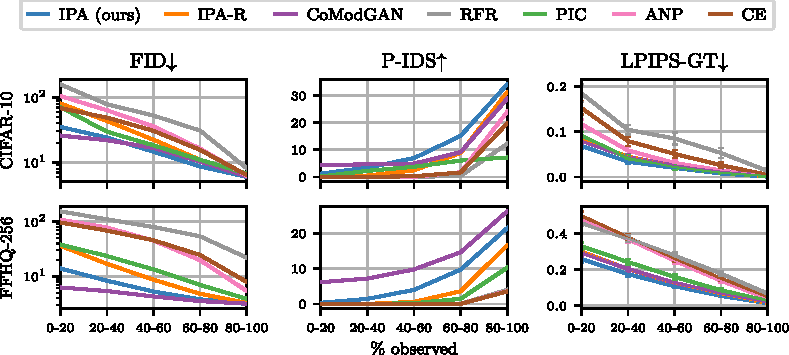
\includegraphics[width=\textwidth]{figs/cigcvae/metrics}
  %\vspace{-.6cm}
  \caption{Image-completion evaluation metrics on CIFAR-10 and FFHQ-256, plotted as a function of the proportion of pixels masked out. Error bars on LPIPS-GT show the standard error of our
    estimate for a single trained network.}
  \label{fig:cigcvae-metrics}
  \vspace{-.5cm}
\end{figure*}


\paragraph{Edges-to-photos}
We provide an additional demonstration of IPA on the Edges2Shoes and
Edges2Handbags datasets~\citep{isola2016image}, where the task is to generate an
image conditioned on the output of an edge detector applied to that image. We
downsample the datasets to $64\times64$ so that we can use unconditional VAEs
pretrained on ImageNet~\citep{deng2009imagenet} at this resolution by
\citet{child2020very}. We show in \cref{fig:cigcvae-training} that IPA is useful for
these tasks, and provide further discussion below. The generated images are
diverse and photorealistic, as shown in \cref{supp:cigcvae-image-samples}.



\begin{figure*}[t]
  \centering
  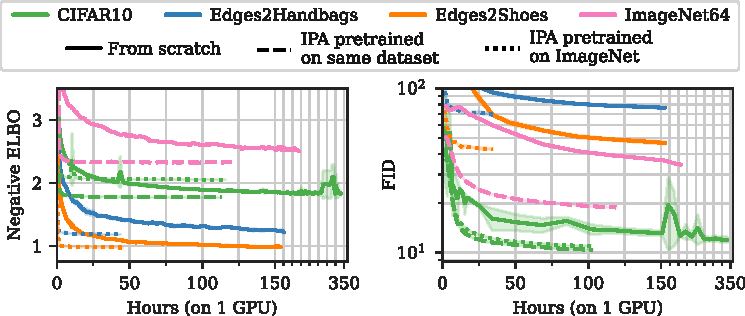
\includegraphics[scale=1]{figs/cigcvae/training-both}
  \caption{Comparison of training from scratch; using IPA starting from an ImageNet-pretrained model; and using IPA starting from a model pretrained on the same dataset. For each, we plot ELBO (\cref{eq:forward-elbo} computed with $\tildeI{} := \rvx$) and FID during training. Error bars show standard deviations computed with 3 runs. Using IPA makes training faster and lower-variance.}
  \label{fig:cigcvae-training}
\end{figure*}

\paragraph{Effectiveness of pretrained weights}
We now seek to determine how important the pretrained unconditional VAE weights
are to IPA. \Cref{fig:cigcvae-training} compares IPA with conditional VAEs which use IPA's architecture
but are trained from scratch, which we will refer to as ``from-scratch''
baselines. In these baselines, $\theta$ and $\phi$ are randomly initialised and trained to
maximise the conditional VAE objective (\cref{eq:forward-elbo}, with $\tildeI{} := \rvx$) along with
$\psi$.
%
With an infinite training budget, the end-to-end training of the from-scratch
baselines is likely to lead them to outperform any IPA models. Nevertheless it
is apparent from \cref{fig:cigcvae-training} that, in the more realistic situation of a
finite training budget, using IPA can be beneficial. This is the case even for
training budgets of up to a few GPU-weeks on the relatively small CIFAR-10
dataset. In fact, even with only a couple of days of training, IPA on CIFAR-10
(with CIFAR-10 pretraining) achieves better FID and ELBO scores than the
from-scratch baseline trained for several weeks. For ImageNet-64, IPA performs
better after 4 hours than the from-scratch baseline does after a week.
%
For Edges2Handbags and Edges2Shoes, training with IPA for 2 days yields
performance similar to or better than training with the from-scratch baseline
for 1 week, as measured by the ELBO. This is despite IPA on these datasets using
a trained ImageNet-64 model rather than a model pretrained on those specific
datasets, supporting our suggestion that the dataset used for pretraining need
not exactly match what IPA is then trained on.
%
Measured by the FID score, IPA's performance is even more appealing: wherever
ELBOs are similar between IPA and the from-scratch baselines, IPA achieves a
significantly better FID score.
%
We see that IPA pretrained on ImageNet is less effective for CIFAR-10
than it is for the edges-to-photos datasets, but it improves on the from-scratch
baseline in terms of ELBO for the first 30 hours of training, and in terms of
FID until the from-scratch baseline is trained for several weeks.

\paragraph{An alternative training objective}
In \cref{tab:cigcvae-results-completion} and \cref{fig:cigcvae-metrics}, we report results for
IPA-R, a variation of IPA with a different training objective corresponding to a
mode-seeking KL divergence. IPA almost always outperforms IPA-R, but we
nonetheless provide a full description of IPA-R in \cref{supp:cigcvae-ipa-r}.




\section{Inpainting for Bayesian experimental design} \label{sec:cigcvae-boed}

In this section, we explore a potential application for stochastic image inpainting that
requires a faithful representation of the posterior $\pdata(\rvx|\rvy,\gY)$.
%
In particular, we consider whether it is possible to automatically target a
chest x-ray at areas most likely to reveal abnormalities. This could avoid the
need to scan the entire chest and so bring benefits including reducing the
patient's radiation exposure.
%
While doing so is not possible with standard x-ray machines (which do not take
multiple scans consecutively), and would need to be extensively validated before
use in a clinical setting, we believe this is a worthwhile avenue to explore.
%
Specifically, our imagined system performs a series of x-ray scans, each
targeted at only a small portion of the area of interest. We can select the
coordinates $\coord_t = (x_t, y_t)$ of the location to scan at each step $t$, and
this selection can be informed by what was observed in the previous scans. The
task we consider is how to select $\coord{}_t$ to be maximally informative. In
particular, assume we wish to infer a variable $v$ representing, e.g., whether
the patient has a particular illness. Bayesian optimal experimental design
(BOED)~\citep{chaloner1995bayesian} provides a framework to select a value of
$\coord{}_t$ that is maximally informative about $v$.
%
It involves taking a Bayesian perspective on the problem of estimating $v$. We
have one posterior distribution over $v$ after taking scans at
$\coord{}_1,\ldots,\coord{}_{t-1}$ and another (typically lower entropy) distribution after
conditioning on a scan at $\coord{}_t$ as well.
%
The \textit{expected information gain}, or EIG, quantifies the utility of the
choice of $\coord{}_t$ as the expected difference in entropy between these two
distributions. Using BOED involves estimating the EIG and selecting the scan
location, $\coord{}_t$, to minimise it.

\begin{figure}[t]
  \centering
  \hspace{-.75cm}
  \begin{minipage}{.4\textwidth}
    \centering
    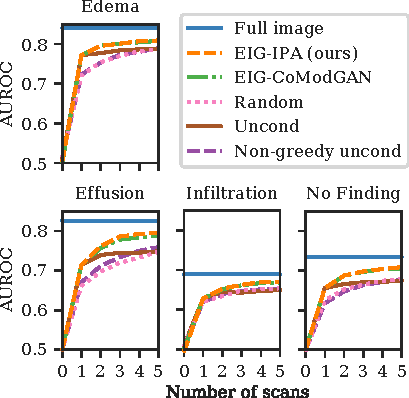
\includegraphics[scale=.77]{figs/cigcvae/boed-auroc-curve-rearranged}
  \end{minipage}
  ~
  \begin{minipage}{0.54\textwidth}
    \centering
    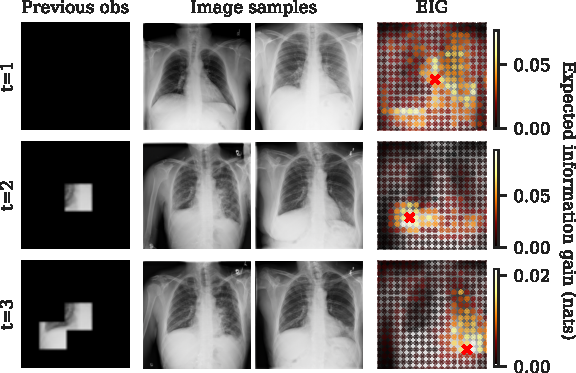
\includegraphics[scale=.77]{figs/cigcvae/shrunk-boed-vis}
  \end{minipage}
  \caption{Evaluation of our IPA-based system for selecting scan locations. \textbf{Left:} Classification AUROC scores after $1,\ldots,5$ scans
    chosen with each method. Scores for the ``EIG-'' methods more quickly approach the
    upper bound achieved by processing the full image. \textbf{Right:}
    Visualisation of IPA used within BOED used to select three scan locations for diagnosing `Effusion'. The left column shows the observations made prior to each time step. We then show samples from IPA (or the dataset when $t=1$). The
    rightmost column shows the EIG overlaid on the pixel-space average of
    sampled images, with the optimal $\coord{}_t$ marked by a red cross.}
  \label{fig:cigcvae-boed}
  \vspace{-.4cm}
\end{figure}



We use an estimator for the EIG similar to that of \citet{harvey2019near}. It
requires two components:
\textbf{(\rom{1})} A neural network trained to classify $v$ given a series of
scans at locations $\coord{}_1,\ldots,\coord{}_t$. This outputs a classification distribution
which we denote $g(v|f_{\coord{}_1,\ldots,\coord{}_t}(\rvx))$, where $f_{\coord{}_1,\ldots,\coord{}_t}$ is a
function mapping from an image to the values of the pixels observed by scans at
$\coord{}_1,\ldots,\coord{}_t$. We use this classification distribution as an approximation of
the posterior over $v$, whose entropy we attempt to minimise by performing BOED.
\textbf{(\rom{2})} A method for sampling image completions conditioned on some
observed pixel values $f_{\coord{}_1,\ldots,\coord{}_{t-1}}(\rvx)$. \citet{harvey2019near}
used a “stochastic image completion” module which contributed significant
complexity to their method. We entirely replace this with IPA.

Let the pixel values observed so far be $\rvy_{\coord{}_1,\ldots,\coord{}_{t-1}} =
f_{\coord{}_1,\ldots,\coord{}_{t-1}}(\rvx)$ for a latent image $\rvx$. Given these, we
estimate the EIG of location $\coord{}_t$ as
\begin{align}
  \label{eq:new-eig}
  \text{EIG}(\coord{}_t;& \rvy_{\coord{}_1,\ldots,\coord{}_{t-1}}) \approx \overbrace{\mathcal{H} \left[ \frac{1}{N} \sum_{n=1}^N g(\cdot|f_{\coord{}_1,\ldots,\coord{}_t}(\rvx^{(n)})) \right]}^{\text{entropy after $t-1$ scans}} - \overbrace{\frac{1}{N} \sum_{n=1}^N  \mathcal{H} \left[ g(\cdot|f_{\coord{}_1,\ldots,\coord{}_t}(\rvx^{(n)})) \right]}^{\text{expected entropy after $t$ scans}},
\end{align}
where $\rvx^{(1)},\ldots,\rvx^{(N)}$ are sampled image inpaintings from IPA
given $\rvy_{\coord{}_1,\ldots,\coord{}_{t-1}}$. In \cref{sec:cigcvae-supp-boed} we report
hyperparameters, provide further details of our EIG estimator, and compare it to
the estimators used in related work. To select $\coord{}_t$, we simply estimate
$\text{EIG}(\coord{}_t; \rvy_{\coord{}_1,\ldots,\coord{}_{t-1}})$ for many different values of
$\coord{}_t$ and select the value which maximises it. This process of selecting $\coord{}_t$
and then taking a scan is repeated for each $t=1,\ldots,T$.

We experiment on the NIH Chest X-ray 14 dataset~\citep{wang2017chestx} at
$256\times256$ resolution.
%
%
% , in which each image is labelled with the presence or
% absence of 14 illnesses. We set $v$ to be a binary label indicating the
% presence/absence of a particular illness. A simple extension, with appropriate
% training data, could be to define $v$ to be the severity of an illness, and
% therefore also infer the severity.
%
We simulate a scanner which returns a $64 \times 64$ pixel patch from this
image, and the task is to diagnose the binary presence or absence of an illness.
We run separate experiments diagnosing each of edema, effusion, infiltration and
``no finding'' (an additional label meaning there are no diagnosed illnesses).
With appropriate data, this framework could be extended to also infer the
severity of a given illness.
%
We envisage BOED being used to select scan locations for an x-ray without
necessarily performing an automated diagnosis. However, to quantify the
informativeness of the chosen locations, \cref{fig:cigcvae-boed} shows the results of
using $g$ to perform a diagnosis, or classification, based on the chosen scan
locations.
%
Since the conditional distribution $g$ (used to estimate the EIG) depends on
which illness we are classifying, the choice of scan locations is different in
each case.
%
We compare against a baseline where the image completion is performed by
CoModGAN (our best-performing image completion baseline) rather than IPA, as
well as numerous baselines which choose scan locations without image
completion; see \cref{sec:cigcvae-supp-boed} for details.

Our method (denoted EIG-IPA) narrowly but consistently outperforms EIG-CoModGAN.
%
% We hypothesise that this is due to CoModGAN's tendency to sometimes produce
% almost no diversity in its completions, even when the observed pixels are
% uninformative.
%
We hypothesise that this is due to the aforementioned tendency of CoModGAN to
sometimes collapse to a single mode of the posterior, and exhibit an example of
this behaviour on the x-ray dataset in \cref{supp:cigcvae-image-samples}. In the BOED
context, such ``overconfident'' image completion could lead to salient scan
locations being ignored. Nonetheless, both EIG-IPA and EIG-CoModGAN
significantly outperform the other baselines, giving performance much closer to
the upper bound of a CNN with access to the entire image. Another benefit of the
``EIG-'' approaches is that the choice of scan locations is highly
interpretable; we can see why a particular location was chosen with
visualisations similar to the right of \cref{fig:cigcvae-boed}. This shows the sampled
images $\rvx^{(n)}$ and the estimated EIG for each $\coord{}_t$. In \cref{sec:cigcvae-supp-boed}, we
show that we can further quantify the contribution of each $\rvx^{(n)}$ to the
estimated EIG for each $\coord{}_t$.

% \section{Discussion and Conclusion}

% We have presented IPA, a method to adapt an unconditional VAE into a conditional
% model. Image completions generated with IPA are close to the state-of-the-art in
% terms of visual fidelity, and improve on all baselines in terms of their
% coverage of the posterior as measured by LPIPS-GT. This high-fidelity coverage
% of the posterior makes IPA ideal for use in Bayesian optimal experimental
% design, as demonstrated.
% %
% % In addition, IPA has all the benefits of a
% % likelihood-based method, such as the potential to perform out-of-distribution
% % detection.
% % 
% \textcolor{black}{ Our theoretical results suggest that, for the applications
%   presented, using the weights of an unconditional VAE is approximately as good
%   as training a conditional VAE from scratch. We note however, that there are
%   applications for which these results will not hold (e.g.~super-resolution).
%   They also provide no guarantees when pretraining is performed on a different
%   dataset, although we show empirically that IPA can still be effective in this
%   case. }
% % 
% Future work may look more rigorously at these settings or further improve the
% image samples by, e.g., using a conditional prior with more expressive
% distributions.
% %
% Preliminary experiments using normalizing flows helped improve the ELBO, but
% with little impact on the FID scores.

\section{Discussion}

We have demonstrated an application of VAEs as flexibly-conditional generative models in the image domain, enabling better handling of uncertainty in image inpainting than prior methods. Doing so involved scaling flexibly-conditional VAEs to higher resolution and more diverse data than prior work~\citep{ivanov2018variational}. The fact that this relatively simple method enabled flexibly conditioning with VAEs also provides a promising signal for the potential to use flexible conditioning with other generative modelling frameworks that may emerge in the future.
%This also serves to show that flexible generative models can be built on the VAE framework as well as on the  diffusion model framework, proving that we are not limited to a single generative modelling framework and providing a positive signal about the potential of combining flexible generative modelling with other frameworks that may show promise in the future.
%\include{relatedwork}
%\include{model}
%\include{impl}
%\include{discussion}
%\chapter{Conclusions and outlook}  \label{ch:conclusion}

In summary, our contributions have demonstrated flexible conditioning with state-of-the-art generative models in a variety of settings.
%
% shows that state-of-the-art generative models can be made flexible, in the sense of being made adaptable to a wide variety of tasks at test-time, with little loss in sample quality. 
%
We found in \cref{ch:fdm} that we could enable flexible conditioning even for very complex and high-dimensional data and, in fact, that the flexible diffusion model which underpins this capability can also improve on the sample quality of standard approaches in such scenarios. Our model generated near-photorealistic video with long-range coherence, outperforming prior work on long-duration video modelling.
%
With the jump diffusion model in \cref{ch:tddm}, we have shown that flexible conditioning is also possible on varying-dimensional data for which we need to model the relationship between the number of dimensions and the conditioning information. We demonstrated this on both molecular data, where it enabled flexible conditioning given a substructure (with potential applications in drug discovery~\citep{hoogeboom2022equivariant}), and video data (where it enabled visual planning even when we do not know how much time it should take to reach the goal frame).
%
Finally, in \cref{ch:cigcvae} we improved upon past implementations of flexible conditioning within the VAE framework. In doing so, we demonstrated image inpainting systems with well-calibrated sample diversity.


\section*{Outlook}

One next step to build on this dissertation would be to simply incorporate recently-proposed methods to speed up sampling. In particular, the diffusion models in \cref{ch:fdm,ch:tddm} both suffer from relatively slow sampling, as do prior diffusion models in other domains~\citep{ho2020denoising,song2020score}. For example, the video model presented in \cref{ch:fdm} took approximately 16 minutes to generate a 300-frame video on a GPU.  Combining our diffusion models with fast samplers like the Heun integrator~\citep{karras2022elucidating} is likely to greatly improve sampling speed at little cost. Incorporating newer approaches like consistency models~\citep{song2023consistency} and rectified flow~\citep{esser2024scaling} could improve speed even further. 

Another clear and promising direction for future research is to scale up the compute resources and amount of data with which we have trained our flexibly-conditional generative models. Perceptual quality and quantitative metrics have both been demonstrated to scale smoothly with compute for images~\citep{peebles2022scalable}; we refer to \citet{esser2024scaling,brooks2024video} for examples of generative models trained with large compute in the image and video domains.

While this thesis focuses on applications in visual domains, we believe that far more domains would benefit from flexibly-conditional diffusion models. For example, we may return to the use-case of a digital twin as mentioned in \cref{ch:introduction}. Consider a digital twin for an engine in which measurements from the real engine deviate from the measurements predicted by its digital twin. This leads the user to suspect a fault in the engine. With a flexibly-conditional model, the user can narrow down what the fault may be as they take more and more relevant measurements by simply conditioning the model on each measurement as they take it. This would not be possible with a standard conditional model unless the set of measurements that could be taken was limited. Diffusion models can be used to model the data obtained from these simulators~\citep{weilbach2023graphically,gloeckler2024all}, enabling our techniques to be incorporated. Data from digital twins is likely be sufficiently complex to require the techniques suggested in \cref{ch:fdm} in addition to potentially being varying-dimensional and needing to be handled using the techniques proposed in \cref{ch:tddm}. Integrating flexibly-conditional models into tools like simulation-based inference software~\citep{gloeckler2024all} could lead to widespread use for such domains.

Next, consider the datasets on which we trained the video model in \cref{ch:fdm}. In each there was a policy for generating the sequences of actions that causally led to the frame-to-frame changes in camera pose. In MineRL the video was generated by agents that were trained to explore novel Minecraft worlds to find a goal block approximately 64 meters away~\citep{saxena2021clockwork}. The CARLA data was produced by a camera attached to an agent driven by a low level proportional–integral–derivative controller following waypoints laid down by a high level planner that was given new, random location goals to
drive to intermittently. In both cases our video model had no access to either the policy or the specific actions taken by these agents and, so, in a formal sense, our models integrate or marginalise over actions drawn from the stochastic policy used to generate the videos in the first place. We posit that our model is likely to also work well if we explicitly model actions and rewards, transforming it video generative model into a vision-based world model in the reinforcement learning sense~\citep{kaiser2019model}. Such a possibility is in addition to the already-demonstrated ability of our model to be conditioned on future frames, which can in principle be up to 100s of frames in the future on CARLA Town01). Combining these capabilities would make it possible to condition on a current and goal frame, and explicitly produce actions to navigate between them.

The above would be a joint vision-action model, but we could also integrate more modalities. For instance, consider a model capable of generating speech and motion data while conditioning on video, input audio, proprioception, etc. It would have the interface needed to operate as an agent in the real world and in principle be capable of performing any tasks a human can perform. Our techniques from \cref{ch:fdm} for generating complex data with bounded compute may be extremely helpful when scaling to model this type of data. Additionally, training on multi-modal data could be made more practical with the proposed flexible diffusion objective (\cref{eq:fdm-loss}) whose task distribution could be made to sometimes drop entire modalities. This would enable training with a mixture of single- and multi-modal data, or on any data source where modalities are sometimes corrupted.




% \section*{Issues with thesis as currently written?}

% \begin{itemize}
%     \item Frank wants more on connections between VAE and diffusion
%     \item finish tables of notation
%     \item check i dont say anything that implies i should have more visual planning results
% \end{itemize}


\clearpage
\chapter{Conclusions and outlook}  \label{ch:conclusion}

In summary, our contributions have demonstrated flexible conditioning with state-of-the-art generative models in a variety of settings.
%
% shows that state-of-the-art generative models can be made flexible, in the sense of being made adaptable to a wide variety of tasks at test-time, with little loss in sample quality. 
%
We found in \cref{ch:fdm} that we could enable flexible conditioning even for very complex and high-dimensional data and, in fact, that the flexible diffusion model which underpins this capability can also improve on the sample quality of standard approaches in such scenarios. Our model generated near-photorealistic video with long-range coherence, outperforming prior work on long-duration video modelling.
%
With the jump diffusion model in \cref{ch:tddm}, we have shown that flexible conditioning is also possible on varying-dimensional data for which we need to model the relationship between the number of dimensions and the conditioning information. We demonstrated this on both molecular data, where it enabled flexible conditioning given a substructure (with potential applications in drug discovery~\citep{hoogeboom2022equivariant}), and video data (where it enabled visual planning even when we do not know how much time it should take to reach the goal frame).
%
Finally, in \cref{ch:cigcvae} we improved upon past implementations of flexible conditioning within the VAE framework. In doing so, we demonstrated image inpainting systems with well-calibrated sample diversity.


\section*{Outlook}

One next step to build on this dissertation would be to simply incorporate recently-proposed methods to speed up sampling. In particular, the diffusion models in \cref{ch:fdm,ch:tddm} both suffer from relatively slow sampling, as do prior diffusion models in other domains~\citep{ho2020denoising,song2020score}. For example, the video model presented in \cref{ch:fdm} took approximately 16 minutes to generate a 300-frame video on a GPU.  Combining our diffusion models with fast samplers like the Heun integrator~\citep{karras2022elucidating} is likely to greatly improve sampling speed at little cost. Incorporating newer approaches like consistency models~\citep{song2023consistency} and rectified flow~\citep{esser2024scaling} could improve speed even further. 

Another clear and promising direction for future research is to scale up the compute resources and amount of data with which we have trained our flexibly-conditional generative models. Perceptual quality and quantitative metrics have both been demonstrated to scale smoothly with compute for images~\citep{peebles2022scalable}; we refer to \citet{esser2024scaling,brooks2024video} for examples of generative models trained with large compute in the image and video domains.

While this thesis focuses on applications in visual domains, we believe that far more domains would benefit from flexibly-conditional diffusion models. For example, we may return to the use-case of a digital twin as mentioned in \cref{ch:introduction}. Consider a digital twin for an engine in which measurements from the real engine deviate from the measurements predicted by its digital twin. This leads the user to suspect a fault in the engine. With a flexibly-conditional model, the user can narrow down what the fault may be as they take more and more relevant measurements by simply conditioning the model on each measurement as they take it. This would not be possible with a standard conditional model unless the set of measurements that could be taken was limited. Diffusion models can be used to model the data obtained from these simulators~\citep{weilbach2023graphically,gloeckler2024all}, enabling our techniques to be incorporated. Data from digital twins is likely be sufficiently complex to require the techniques suggested in \cref{ch:fdm} in addition to potentially being varying-dimensional and needing to be handled using the techniques proposed in \cref{ch:tddm}. Integrating flexibly-conditional models into tools like simulation-based inference software~\citep{gloeckler2024all} could lead to widespread use for such domains.

Next, consider the datasets on which we trained the video model in \cref{ch:fdm}. In each there was a policy for generating the sequences of actions that causally led to the frame-to-frame changes in camera pose. In MineRL the video was generated by agents that were trained to explore novel Minecraft worlds to find a goal block approximately 64 meters away~\citep{saxena2021clockwork}. The CARLA data was produced by a camera attached to an agent driven by a low level proportional–integral–derivative controller following waypoints laid down by a high level planner that was given new, random location goals to
drive to intermittently. In both cases our video model had no access to either the policy or the specific actions taken by these agents and, so, in a formal sense, our models integrate or marginalise over actions drawn from the stochastic policy used to generate the videos in the first place. We posit that our model is likely to also work well if we explicitly model actions and rewards, transforming it video generative model into a vision-based world model in the reinforcement learning sense~\citep{kaiser2019model}. Such a possibility is in addition to the already-demonstrated ability of our model to be conditioned on future frames, which can in principle be up to 100s of frames in the future on CARLA Town01). Combining these capabilities would make it possible to condition on a current and goal frame, and explicitly produce actions to navigate between them.

The above would be a joint vision-action model, but we could also integrate more modalities. For instance, consider a model capable of generating speech and motion data while conditioning on video, input audio, proprioception, etc. It would have the interface needed to operate as an agent in the real world and in principle be capable of performing any tasks a human can perform. Our techniques from \cref{ch:fdm} for generating complex data with bounded compute may be extremely helpful when scaling to model this type of data. Additionally, training on multi-modal data could be made more practical with the proposed flexible diffusion objective (\cref{eq:fdm-loss}) whose task distribution could be made to sometimes drop entire modalities. This would enable training with a mixture of single- and multi-modal data, or on any data source where modalities are sometimes corrupted.




% \section*{Issues with thesis as currently written?}

% \begin{itemize}
%     \item Frank wants more on connections between VAE and diffusion
%     \item finish tables of notation
%     \item check i dont say anything that implies i should have more visual planning results
% \end{itemize}



%    3. Notes
%    4. Footnotes

%    5. Bibliography
\begin{singlespace}
\raggedright
\bibliographystyle{apalike}  %abbrvnat}
\bibliography{biblio}
\end{singlespace}

\appendix
%    6. Appendices (including copies of all required UBC Research
%       Ethics Board's Certificates of Approval)
%\include{reb-coa}	% pdfpages is useful here
% \chapter{Supporting Materials}
\chapter{Diffusion models}

\chapter{Score-matching objective derivation} \label{sec:proof-that-diffusion-does-score-matching}

\begin{align}
\allowdisplaybreaks
S(\theta, t) &= \EX_{q(\rvx_t, \rvy)} \left[ - 2 \left\langle \nabla_{\rvx_t} \log q(\rvx_t|\rvy)^\top, \rvs_\theta(\rvx_t, \rvy, \sigma) \right\rangle \right] \\
    &= \EX_{\pdata(\rvy)}\left[  - 2 \int q(\rvx_t | \rvy) \left\langle \nabla_{\rvx_t} \log q(\rvx_t | \rvy), \rvs_\theta(\rvx_t, \rvy, \sigma) \right\rangle \mathrm{d} \rvx_t \right] \\
    &= \EX_{\pdata(\rvy)}\left[ - 2 \int q(\rvx_t | \rvy) \left\langle \frac{\nabla_{\rvx_t} q(\rvx_t|\rvy)}{q(\rvx_t | \rvy)}, \rvs_\theta(\rvx_t, \rvy, \sigma) \right\rangle \mathrm{d} \rvx_t \right] \\
    &= \EX_{\pdata(\rvy)}\left[  - 2 \int \left\langle \nabla_{\rvx_t} q(\rvx_t | \rvy), \rvs_\theta(\rvx_t, \rvy, \sigma) \right\rangle \mathrm{d} \rvx_t \right] \\
    &= \EX_{\pdata(\rvy)}\left[  - 2 \int \left\langle \nabla_{\rvx_t} \int \pdata(\rvx_0|\rvy) q(\rvx_t|\rvx_0) \mathrm{d}\rvx_0, \rvs_\theta(\rvx_t, \rvy, \sigma) \right\rangle \mathrm{d} \rvx_t \right] \\
    &= \EX_{\pdata(\rvy)}\left[  - 2 \int \left\langle \int \pdata(\rvx_0|\rvy) \nabla_{\rvx_t} q(\rvx_t|\rvx_0) \mathrm{d}\rvx_0, \rvs_\theta(\rvx_t, \rvy, \sigma) \right\rangle \mathrm{d} \rvx_t \right] \\
    &= \EX_{\pdata(\rvy)}\left[  - 2 \int \left\langle \int \pdata(\rvx_0|\rvy) q(\rvx_t|\rvx_0) \nabla_{\rvx_t} \log q(\rvx_t|\rvx_0) \mathrm{d}\rvx_0, \rvs_\theta(\rvx_t, \rvy, \sigma) \right\rangle \mathrm{d} \rvx_t \right] \\
    &= \EX_{\pdata(\rvy)}\left[  - 2 \int q(\rvx_0, \rvx_t|\rvy) \left\langle \nabla_{\rvx_t} \log q(\rvx_t|\rvx_0), \rvs_\theta(\rvx_t, \rvy, \sigma) \right\rangle  \mathrm{d}\rvx_0 \mathrm{d} \rvx_t \right] \\
    &= \EX_{q(\rvx_0, \rvx_t, \rvy)} \left[ -2 \left\langle \nabla_{\rvx_t} \log q(\rvx_t|\rvx_0), \rvs_\theta(\rvx_t, \rvy, \sigma) \right\rangle  \right]
\end{align}

\chapter{Supporting materials for flexibly-conditional variational auto-encoders}

% \section{Notation}
% We provide \cref{tab:cigcvae-notation} for reference as a concise list of definitions
% for each symbol used in our discussion of hierarchical VAEs. 

\section{Expanded derivation of IPA's objective} \label{supp:cigcvae-forward-elbo-bound-deriv}
Here we prove \cref{eq:forward-elbo}, which states that IPA's training
objective is a lower bound on $\EX_{\pdata (\rvx, \rvy)} \left[ \log
  p_{\theta,\psi}(\tildeI{}|\rvy) \right]$.
\begin{align}
  \gO_\text{CVAE}(\theta, \phi, \psi ) &= \EX_{\pdata (\rvx, \rvy)} \EX_{q_\phi(\rvz|\rvx)} \left[ \log \frac{p_\theta(\tildeI{}|\rvz)p_\psi(\rvz|\rvy)}{q_\phi(\rvz|\rvx)} \right] \\
                                                   &\leq \EX_{\pdata (\rvx, \rvy)} \left[ \log \EX_{q_\phi(\rvz|\rvx)} \left[ \frac{p_\theta(\tildeI{}|\rvz)p_\psi(\rvz|\rvy)}{q_\phi(\rvz|\rvx)} \right]  \right] \\
                                                   &= \EX_{\pdata (\rvx, \rvy)} \left[ \log \EX_{p_\psi(\rvz|\rvy)} \left[ p_\theta(\tildeI{}|\rvz) \right]  \right] \\
                                                   &= \EX_{\pdata (\rvx, \rvy)} \left[ \log p_{\theta,\psi}(\tildeI{}|\rvy) \right],
\end{align}
where the final step follows from the definition of $p_{\theta,\psi}$ in
\cref{eq:marginal-image-posterior}.


\section{Proof and discussion of Theorem~\ref{theorem:forward-kl}} \label{proof:forward-kl}
\subsection{Proof}
\textbf{Statement.}
\textit{
  For any set $\Psi$ of
  permissible values of $\psi $, and for any $\theta\in\Theta$ and
  $\phi\in\Phi$,
  \begin{equation}
    \argmax_{\psi  \in \Psi} \gO_\text{CVAE}(\theta, \phi, \psi ) = \argmin_{\psi  \in \Psi} \EX_{\pdata (\rvy)} \left[ \kl[\big]{ q_\phi(\rvz|\rvy) }{ p_\psi(\rvz|\rvy) } \right]. \tag{\ref{eq:forward-theorem}}
  \end{equation}
}

\textbf{Proof.} We can decompose $\gO_\text{CVAE}$ as follows.
Starting by multiplying both sides of the fraction by the intractable
conditional distribution $q_\phi(\rvz|\rvy)$,
\begin{align}
  \gO_\text{CVAE}(\theta, \phi, \psi ) &= \EX_{q_\phi(\rvz,\rvx,\rvy)} \left[ \log \frac{p_\theta(\tildeI{}|\rvz)p_\psi(\rvz|\rvy)q_\phi(\rvz|\rvy)}{q_\phi(\rvz|\rvx)q_\phi(\rvz|\rvy)} \right]\\
                                                   &= \EX_{q_\phi(\rvz,\rvx,\rvy)} \left[ \log \frac{p_\theta(\tildeI{}|\rvz)q_\phi(\rvz|\rvy)}{q_\phi(\rvz|\rvx)} \right] - \EX_{q_\phi(\rvz,\rvy)} \left[ \log\frac{q_\phi(\rvz|\rvy)}{p_\psi(\rvz|\rvy)} \right] \\
                                                   &= C(\theta, \phi) - \EX_{\pdata (\rvy)} \left[ \kl[\big]{ q_\phi(\rvz|\rvy) }{ p_\psi(\rvz|\rvy) } \right]   \label{eq:constant-and-forward-kl}
\end{align}
where $C(\theta, \phi)$ is a grouping of terms which do not depend on the
partial encoder's parameters $\psi $. Any values of $\psi$ which
maximise $\gO_\text{CVAE}(\theta, \phi, \psi)$ will therefore also
minimise $\EX_{\pdata (\rvy)} \left[ \kl[\big]{ q_\phi(\rvz|\rvy) }{p_\psi(\rvz|\rvy) } \right]$ for the same values of $\theta$ and $\phi$,
which proves the theorem.

\subsection{Bound on data-space divergence}
The mass-covering KL divergence in \Cref{theorem:forward-kl} indicates that
samples $\rvz\sim p_\psi(\cdot|\rvy)$ will be diverse (when $q_\phi(\rvz|\rvy)$ is
diverse/uncertain). One would expect that samples of $\tildeI{}$ conditioned on these
diverse samples of $\rvz$ will also be diverse. Here we make a more formal argument
by showing that minimising $\gO_\text{CVAE}$ corresponds to minimising
an upper-bound on an expected mass-covering KL divergence in $\tildeI{}$-space.
Starting from the result in \cref{supp:cigcvae-forward-elbo-bound-deriv},
\begin{align}
  &\gO_\text{CVAE}(\theta, \phi, \psi ) \\
  \leq &\EX_{\pdata (\rvx,\rvy)} \left[ \log p_{\theta,\psi}(\tildeI{}|\rvy) \right] \\
  = &\EX_{\pdata (\rvx,\rvy)} \left[ \log \pdata (\tildeI{}|\rvy) \right] - \EX_{\pdata (\rvy)}\left[ \kl{\pdata (\tildeI{}|\rvy)}{p_{\theta,\psi}(\tildeI{}|\rvy)} \right].
\end{align}
Rearranging this gives
\begin{align}
  \EX_{\pdata (\rvy)}\left[ \kl{\pdata (\tildeI{}|\rvy)}{p_{\theta,\psi}(\tildeI{}|\rvy)} \right]  \leq \EX_{\pdata (\rvx,\rvy)} \left[ \log \pdata (\tildeI{}|\rvy) \right] - \gO_\text{CVAE}(\theta, \phi, \psi ).
\end{align}
Maximising $\gO_\text{CVAE}$ therefore minimises an upper-bound on an
expected mass-covering KL divergence in $\tildeI{}$-space, providing a further suggestion that
$\tildeI{}\sim p_{\theta,\psi}(\cdot|\rvy)$ will be diverse.

\section{Simplifications with optimal parameters}

In this section we introduce a lemma and notation that will be useful in later proofs.

\begin{theorem} \label{theorem:optimal-distributions-equal}
    Assume that we have a sufficiently expressive
  encoder and decoder that there exist parameters $\optimal{\theta}\in\Theta$
  and $\optimal{\phi}\in\Phi$ which make the unconditional VAE objective
  (\cref{eq:vae-objective}) equal to its upper bound of $-\mathcal{H}\left[ \pdata(\rvx)
  \right]$. Then,
\begin{equation} \label{eq:optimal-distributions-equal}
  p_{\optimal{\theta}}(\rvx,\rvy,\rvz) = q_{\optimal{\phi}}(\rvx,\rvy,\rvz)
\end{equation}
\end{theorem}

\textbf{Proof.} Recall the definitions of $p$ and $q$ in \cref{eq:pmodel,eq:r}, which are $p_{\optimal{\theta}}(\rvx,\rvy,\rvz) = p_{\optimal{\theta}}(\rvx|\rvz)p_{\optimal{\theta}}(\rvz)\pdata(\rvy|\rvx)$ and $q_{\optimal{\phi}}(\rvx,\rvy,\rvz) = \pdata(\rvx,\rvy)q_{\optimal{\phi}}(\rvz|\rvx)$. Both contain a factor of $\pdata(\rvy|\rvx)$, so we can prove \cref{theorem:optimal-distributions-equal} by proving the simplified equality $p_{\optimal{\theta}}(\rvx,\rvz) = \pdata(\rvx) q_{\optimal{\phi}}(\rvz|\rvx)$. We can do so by representing the unconditional VAE objective similar to the conditional VAE objective in \cref{eq:elbo-kl-joints}, e.g. by substituting $\rvy = \varnothing$ into \cref{eq:elbo-kl-joints}, giving
\begin{equation}
    \EX_{\pdata(\rvx)} \left[ \gL(\rvx,\optimal{\theta},\optimal{\phi}) \right] =  - \gH \left[ \pdata(\rvx) \right] 
    - \kl{ \pdata(\rvx)q_{\optimal{\phi}}(\rvz|\rvx) 
    }{
    p_{\optimal{\theta}}(\rvx,\rvz) 
    }.
\end{equation}
Given our assumption that the objective is made equal to $- \gH \left[ \pdata(\rvx) \right]$ with parameters $\theta$ and $\phi$, the KL divergence must be zero. This implies that $p_{\optimal{\theta}}(\rvx,\rvz) = \pdata(\rvx)q_{\optimal{\phi}}(\rvz|\rvx) $, proving the theorem.

For convenience we now define $\unp(\rvx,\rvy,\rvz)$ to be equal to both sides of \cref{eq:optimal-distributions-equal}. That is, $\unp(\rvx,\rvy,\rvz) = p_{\optimal{\theta}}(\rvx,\rvy,\rvz) = q_{\optimal{\phi}}(\rvx,\rvy,\rvz)$. We note that we can also write the joint
distribution $\optimal{p}(\rvz, \rvx, \tildeI{}, \rvy) = \pdata (\rvx,
\rvy) q_\phi(\rvz|\rvx; \optimal{\phi})p(\tildeI{}|\rvx,\rvy)$, where
$p(\tildeI{}|\rvx,\rvy)=\delta_{g(\rvx,\rvy)}(\tildeI{})$ is the Dirac
distribution mapping $\rvx$ and $\rvy$ deterministically to
$\tildeI{}=g(\rvx,\rvy)$.

\section{Proof and discussion of Theorem~\ref{theorem:joint-training}}  \label{proof:joint-training}

\subsection{Proof}

\textbf{Statement.} \textit{Assume that we have a sufficiently expressive
  encoder and decoder that there exist parameters $\optimal{\theta}\in\Theta$
  and $\optimal{\phi}\in\Phi$ which make the unconditional VAE objective
  (\cref{eq:vae-objective}) equal to its upper bound of $-\mathcal{H}\left[ \pdata(\rvx)
  \right]$. Assume also that the mutual information ${\mutinf{} :=
  \EX_{p_{\theta^*}(\tildeI{}, \rvy, \rvz)} \left[ \log
    \frac{p_{\theta^*}(\tildeI{},\rvy|\rvz) }{ p_{\theta^*}(\tildeI{}|\rvz)p_{\theta^*}(\rvy|\rvz) } \right] =
  \EX_{p_{\theta^*}(\tildeI{}, \rvy, \rvz)} \left[ \log
    \frac{p_{\theta^*}(\tildeI{}|\rvz, \rvy) }{ p_{\theta^*}(\tildeI{}|\rvz) } \right]}$ is zero (meaning that $\tildeI{}$ and $\rvy$ are
  conditionally independent given $\rvz$) and $\tildeI{}$ is defined such that there
  exists a mapping from $(\tildeI{},\rvy)$ to $\rvx$. Then, given a
  sufficiently expressive partial encoder $p_\psi(\rvz|\rvy; \psi)$, }
\begin{equation} \tag{\ref{eq:joint-training}}
  \max_{\psi } \gO_\text{CVAE}(\optimal{\theta}, \optimal{\phi}, \psi ) = \max_{\theta, \phi, \psi } \gO_\text{CVAE}(\theta, \phi, \psi ).
\end{equation}

\textbf{Proof.} 
% We have used, and will continue to use, $p_\theta(\cdot)$ and
% $q_\phi(\cdot)$ to refer to joint distributions parameterised by $\theta$ and $\phi$
% respectively. Since $\optimal{\theta}$ and $\optimal{\phi}$ are defined as the
% maximisers of the unconditional ELBO in \cref{eq:elbo-kl-joints}, and given our
% assumption of sufficient expressivity, we have $p_{\optimal{\theta}}(\rvz, \rvx) = \pdata(\rvx) q_{\optimal{\phi}}(\rvz|\rvx)$. We can therefore
% introduce notation for the equal joint distributions: $\optimal{p}(\rvz, \rvx,
% \rvy) = p_\theta(\rvz, \rvx, \rvy; \optimal{\theta}) = \pdata (\rvx,
% \rvy) q_\phi(\rvz|\rvx; \optimal{\phi})$. 
% %
% Recalling that we define $\tildeI{}$ as either equal to $\rvx$ or as the
% dimensions of $\rvx$ not observed in $\rvy$, such a deterministic $g$ will
% always exist.
We consider the decomposition of $\gO_\text{CVAE}$ shown in
\cref{eq:constant-and-forward-kl} and remind the reader that, given a
sufficiently expressive partial encoder, the maximisation over $\psi$ will
always make the KL divergence zero. That is,
\begin{equation}
  \max_{\psi } \gO_\text{CVAE}(\theta, \phi, \psi ) = C(\theta, \phi) = \EX_{q_\phi(\rvz,\rvx,\rvy)} \left[ \log \frac{p_\theta(\tildeI{}|\rvz)q_\phi(\rvz|\rvy)}{q_\phi(\rvz|\rvx)} \right] \label{eq:forward-max-phi}
\end{equation}
for any $\theta$ and $\phi$. Using $\optimal{\theta}$ and $\optimal{\phi}$, and
therefore using $\unp{}$ in place of $p_\theta$, $r$ and $q$, we can expand the
left-hand side of \cref{eq:joint-training}.
\begin{align}
  \max_{\psi } \gO_\text{CVAE}(\optimal{\theta}, \optimal{\phi}, \psi ) &= \EX_{\unp{}(\rvz,\rvx,\rvy)} \left[ \log \frac{\unp{}(\tildeI{}|\rvz)\unp{}(\rvz|\rvy)}{\unp(\rvz|\rvx)} \right] \\
                                                   &= \EX_{\unp{}(\rvz,\rvx,\rvy)} \left[ \log \frac{\unp{}(\tildeI{}|\rvz,\rvy)\unp{}(\rvz|\rvy)}{\unp(\rvz|\rvx)} \right] \nonumber \\
                                                   & \quad - \EX_{\unp{}(\rvz,\tildeI{},\rvy)} \left[ \log\frac{\unp{}(\tildeI{}|\rvz,\rvy)}{\unp{}(\tildeI{}|\rvz)} \right] \\
                                                   &= \EX_{\unp{}(\rvz,\rvx,\rvy)} \left[ \log \frac{\unp{}(\tildeI{}|\rvz,\rvy)\unp{}(\rvz|\rvy)}{\unp(\rvz|\rvx)} \right] - \mutinf{}\\
                                                                                           &= \EX_{\unp{}(\rvz,\rvx,\rvy)} \left[ \log \frac{\unp{}(\rvz,\tildeI{}|\rvy)}{\unp(\rvz|\rvx)} \right] - \mutinf{}\\
                                                                                           &= \EX_{\unp{}(\rvz,\rvx,\rvy)} \left[ \log \frac{\unp{}(\rvz|\tildeI{},\rvy)\unp{}(\tildeI{}|\rvy)}{\unp(\rvz|\rvx)} \right] - \mutinf{}. \label{eq:pre-mapping}
\end{align}
The factorisation $\optimal{p}(\rvz, \rvx, \tildeI{}, \rvy) = \pdata (\rvx,
\rvy) q_\phi(\rvz|\rvx; \optimal{\phi})\delta(\tildeI{}|\rvx,\rvy)$ implies that
we can express $\unp{}(\rvz|\tildeI{},\rvy)$ with a marginalisation:
$\unp{}(\rvz|\tildeI{},\rvy)=\int \unp{}(\rvz|\rvx)
\unp{}(\rvx|\tildeI{},\rvy) \mathrm{d}\rvx$. Since we have assumed that
there is a deterministic function $f$ mapping $(\tildeI{},\rvy)$ to $\rvx$,
$\unp{}(\rvx|\tildeI{},\rvy)$ is a Dirac distribution and the
marginalisation becomes $\unp{}(\rvz|\tildeI{},\rvy) = \int \unp{}(\rvz|\rvx)
\delta(\rvx|\tildeI{},\rvy) \mathrm{d}\rvx =
\unp{}(\rvz|\rvx=f(\tildeI{},\rvy))$. We therefore proceed, rewriting
$\unp{}(\rvz|\tildeI{},\rvy)$ as $\unp{}(\rvz|\rvx)$:
\begin{align}
  \max_{\psi } \gO_\text{CVAE}(\optimal{\theta}, \optimal{\phi}, \psi ) &= \EX_{\unp{}(\rvz,\rvx,\rvy)} \left[ \log \frac{\unp{}(\rvz|\rvx)\unp{}(\tildeI{}|\rvy)}{\unp(\rvz|\rvx)} \right] - \mutinf{} \label{eq:post-mapping}\\
                                                                                           &= \EX_{\unp{}(\rvx,\rvy)} \left[ \log \unp{} (\tildeI{}|\rvy) \right] - \mutinf{}\\
                                                                                           &= \EX_{\pdata (\rvx,\rvy)} \left[ \log \pdata  (\tildeI{}|\rvy) \right] - \mutinf{}. \label{eq:max-partphi-bound}
\end{align}
Now that we have this expansion of the left-hand side of
\cref{eq:joint-training}, we can derive a related upper-bound on the right-hand
side as follows. For any $\theta$, any $\phi$, and any $\psi$, we have
from \cref{supp:cigcvae-forward-elbo-bound-deriv}:
\begin{align}
  \gO_\text{CVAE}(\theta, \phi, \psi ) &\leq \EX_{\pdata (\rvx,\rvy)} \left[ \log p_{\theta,\psi}(\tildeI{}|\rvy) \right] \\
                                                     &= \EX_{\pdata (\rvx,\rvy)} \left[ \log \pdata (\tildeI{}|\rvy) \right] - \EX_{\pdata (\rvy)}\left[ \kl{\pdata (\tildeI{}|\rvy)}{p_{\theta,\psi}(\tildeI{}|\rvy)} \right] \\
                                                     &\leq \EX_{\pdata (\rvx,\rvy)} \left[ \log \pdata (\tildeI{}|\rvy) \right].
\end{align}
This bound must also hold for the maximum over $\theta$, $\phi$, and
$\psi$, and so is an upper-bound on the right-hand side of \cref{eq:joint-training}:
\begin{align}
  \max_{\theta, \phi, \psi } \gO_\text{CVAE}(\theta, \phi, \psi ) &\leq \EX_{\pdata (\rvx,\rvy)} \left[ \log \pdata (\tildeI{}|\rvy) \right]. \label{eq:max-all-bound}
\end{align}

By relating \cref{eq:max-partphi-bound} and \cref{eq:max-all-bound}, we have:
\begin{align}
  \max_{\theta, \phi, \psi } \gO_\text{CVAE}(\theta, \phi, \psi ) &\leq  \max_{\psi } \gO_\text{CVAE}(\optimal{\theta}, \optimal{\phi}, \psi ) + \mutinf{}. \label{eq:bound-1}
\end{align}
We then point out that we can also obtain an inequality in the other direction: since
the right-hand side of \cref{eq:joint-training} is a maximisation of the left-hand side over $\theta$ and
$\phi$, it must be greater than or equal to the left-hand side:
\begin{align}
  \max_{\psi } \gO_\text{CVAE}(\optimal{\theta}, \optimal{\phi}, \psi ) &\leq  \max_{\theta, \phi, \psi } \gO_\text{CVAE}(\theta, \phi, \psi )  . \label{eq:bound-2}
\end{align}
Combining \cref{eq:bound-1} and \cref{eq:bound-2}, we have:
\begin{align}
  0 \leq \max_{\theta, \phi, \psi } \gO_\text{CVAE}(\theta, \phi, \psi ) - \max_{\psi } \gO_\text{CVAE}(\optimal{\theta}, \optimal{\phi}, \psi ) \leq \mutinf{}. \label{eq:two-bounds}
\end{align}
We now have bounds in both directions on the difference between the right- and
left-hand sides. To conclude the proof, we repeat the assumption that
$\mutinf{}=0$. The upper- and lower- bounds of \cref{eq:two-bounds} are
therefore both zero, so we have the final result that ${\max_{\psi }
\gO_\text{CVAE}(\optimal{\theta}, \optimal{\phi}, \psi ) =
\max_{\theta, \phi, \psi } \gO_\text{CVAE}(\theta, \phi,
\psi )}$.

\subsection{Discussion of the assumption of zero mutual information}
The above proof of \cref{theorem:joint-training} relies on the assumption that
\begin{equation}
    \mutinf{} = \EX_{\unp{}(\tildeI{}, \rvy, \rvz)} \left[ \log \frac{\unp{}(\tildeI{}|\rvz, \rvy) }{ \unp{}(\tildeI{}|\rvz) } \right] = 0.    
\end{equation}
That is, that under the joint distribution $p_{\theta^*,\phi^*}(\rvz,\rvx,\rvy)$, $\tildeI{}$ and
$\rvy$ should be conditionally independent given $\rvz$. We now argue that this
is true for image completion, and ``close to'' satisfied \textcolor{black}{when
  $\mathbf{y}$ consists of high-level image features. This means that
  \cref{theorem:joint-training} is informative for inpainting, our
  edges-to-photos experiments and, e.g., class-conditional generation but may
  not even approximately hold for, e.g., super-resolution or image
  colourisation.}

\paragraph{Image completion}
In the VAE architecture we use, the likelihood $p_\theta(\rvx|\rvz)$ is pixel-wise
independent. In other words, if we write $\rvx$ as a set of pixels
$\{\rvx_1,\ldots,\rvx_N\}$, we can factorise $p_\theta(\rvx|\rvz)$ as
$\prod_{i=1}^Np_\theta(\rvx_i|\rvz)$. This means that the conditional mutual
information between any two disjoint subsets of $\rvx$ (conditioned on $\rvz$) will
be zero. Given our definition of $\tildeI{}$ for image completion as the the set
of purely unobserved pixels, we have by construction that $\tildeI{}$ and
$\rvy$ are disjoint. Therefore, the assumption that $\mutinf{}=0$ is
satisfied for image completion.


\paragraph{When $\mutinf{}$ is non-zero.}
When $\mutinf{}$ is non-zero, we can still use it as an upper-bound on the
difference between the left- and right-hand side of \cref{eq:joint-training}
using \cref{eq:two-bounds}.
%
Moreover, we posit that $\mutinf{}$ will typically be small when $\rvy$
represents high-level features (e.g.~the edges in Edges2Photos or a class label)
and we have a pixel-wise independent likelihood. This is because any high-level
structure cannot be modelled by the pixel-wise independent likelihood
$\unp{}(\tildeI{}|\rvz)$ and so must be captured by $\rvz$. Intuitively, high-level
features $\rvy$ are unlikely to be informative about any pixel-level
variations if all image structure spanning multiple pixels ($\rvz$) is already
known. This is equivalent to saying that $\mutinf{}$, the mutual information
between $\tildeI{}$ and $\rvy$ conditioned on $\rvz$, is likely to be small.

\section{An alternative training objective}
\label{supp:cigcvae-ipa-r}
In this section, we describe an alternative objective previously used by
\citet{ma2018eddi}. We find experimentally that its performance is typically
worse than $\gO_\text{CVAE}$, but it has the advantage of only
requiring data $\rvy \sim \pdata (\cdot)$ during training, and not $\rvx$.
This may allow training in settings such as
outpainting~\citep{sabini2018painting}. The objective can be interpreted as a
lower bound on $\log p_\theta(\rvy)$:
\begin{align} \label{eq:reverse-obj}
  \mathcal{O}_\text{rev}(\theta, \phi, \psi ) &= \EX_{\pdata (\rvy)}\EX_{p_\psi(\rvz|\rvy)} \left[ \log\frac{p_\theta(\rvz,\rvy)}{p_\psi(\rvz|\rvy)} \right] \leq \EX_{\pdata (\rvy)} \left[ \log p_\theta(\rvy) \right].
\end{align}
Computing this objective requires a computation graph similar to that shown in
\cref{fig:cigcvae-reverse-arch}. Note one caveat with this objective is that using it
involves computing and differentiating $p_\theta(\rvz,\rvy)$, which requires a
tractable likelihood $\pdata (\rvy|\rvx)$ (based on the definition of
$p_\theta$ in \cref{tab:notation-appendix-cigcvae}). This is possible in image completion, but
not in the general case of conditional generation.

The following theorem says that learning $\psi $ to maximise this objective
is equivalent to minimising another KL divergence.
\begin{theorem} \label{theorem:reverse-kl} For any set $\Psi$ of
  permissible values of $\psi $, and for any $\theta\in\Theta$ and
  $\phi\in\Phi$,
  \begin{equation}
    \argmax_{\psi  \in \Psi} \mathcal{O}_\text{rev}(\theta, \phi, \psi ) = \argmin_{\psi  \in \Psi} \EX_{\pdata (\rvy)} \left[ \kl[\big] { p_\psi(\rvz|\rvy; \psi) }{ p_\theta(\rvz|\rvy; \theta) } \right].
  \end{equation}
\end{theorem}


\textbf{Proof.}
We show this by decomposing the objective:
\begin{align} \label{eq:reverse-obj-supp}
  \mathcal{O}_\text{rev}(\theta, \phi, \psi ) &= \EX_{\pdata (\rvy)p_\psi(\rvz|\rvy)} \left[ \log\frac{p_\theta(\rvz,\rvy)}{p_\psi(\rvz|\rvy)} \right] \\
                                                   &= \EX_{\pdata (\rvy)p_\psi(\rvz|\rvy)}\Big[ \log p_\theta(\rvy) - \log\frac{p_\psi(\rvz|\rvy)}{p_\theta(\rvz|\rvy)} \Big] \\
  &= \EX_{\pdata (\rvy)}\Big[ \log p_\theta(\rvy) - \kl[\big] { p_\psi(\rvz|\rvy) }{ p_\theta(\rvz|\rvy) } \Big] \\
                                                   &= D(\theta) - \EX_{\pdata (\rvy)}\Big[ \kl[\big] { p_\psi(\rvz|\rvy) }{ p_\theta(\rvz|\rvy) } \Big]
\end{align}
where $D(\theta)$ is not dependent on $\psi$. Therefore, for any $\theta$
and $\phi$, any values of $\psi\in\Psi$ which maximise
$\mathcal{O}_\text{rev}(\theta, \phi, \psi )$ will equivalently minimise the expression
$\EX_{\pdata (\rvy)}\Big[ \kl[\big] { p_\psi(\rvz|\rvy) }{
  p_\theta(\rvz|\rvy) } \Big]$,
  proving the theorem.


\Cref{theorem:reverse-kl} implies that maximising $\mathcal{O}_{\text{rev}}$
will minimise a ``reverse'' KL divergence (hence its name $\mathcal{O}_{\text{rev}}$), causing $p_\psi(\rvz|\rvy)$ to
exhibit mode-seeking behaviour. We denote the method of training with this
objective IPA-R (inference in a pretrained artifact with the reverse KL).
                                                     %
As with IPA, we use pretrained $\theta$ and $\phi$ when training IPA-R, which we
justify in the following paragraph. With IPA-R, we also use the pretrained
encoder parameters $\phi$ as an initialisation for $\psi $, which makes
training more stable.

% \paragraph{Using pretrained weights with $\mathcal{O}_\text{rev}$}
To justify the use of a pretrained $\theta$ and $\phi$ with
$\mathcal{O}_\text{rev}$, we show that the objective $\mathcal{O}_\text{rev}$
has a property analogous to that described by \cref{theorem:joint-training}.
\begin{theorem}
  \label{theorem:joint-training-rev}
  Assume we have a sufficiently expressive encoder and decoder such that there
  exists parameters $\optimal{\theta}\in\Theta$ and $\optimal{\phi}\in\Phi$
  which make the unconditional VAE objective equal to its
  upper bound of $-\mathcal{H}\left[ \pdata(\rvx) \right]$. Then, given a
  sufficiently expressive partial encoder $p_\psi(\rvz|\rvy; \psi)$,
  \begin{equation*}
    \max_{\psi } \mathcal{O}_\text{rev}(\optimal{\theta}, \optimal{\phi}, \psi ) = \max_{\theta, \phi, \psi } \mathcal{O}_\text{rev}(\theta, \phi, \psi ).
  \end{equation*}
\end{theorem}

\textbf{Proof.} We will prove \cref{theorem:joint-training-rev} by showing that
both the quantity on the left-hand side and the quantity on the right-hand side
are equal to the negative of the entropy of $\pdata (\rvx)$. We begin with the
left-hand side,
\begin{align}
  \max_{\psi } \mathcal{O}_\text{rev}(\optimal{\theta}, \optimal{\phi}, \psi ) &= \max_{\psi } \EX_{\pdata (\rvy)p_\psi(\rvz|\rvy)} \left[ \log\frac{\unp{}(\rvz,\rvy)}{p_\psi(\rvz|\rvy)} \right].
\end{align}
This is a variational lower-bound which is made tight by setting $\psi $
such that $p_\psi(\rvz|\rvy) = \unp{}(\rvz|\rvy)$:
\begin{align}
  \max_{\psi } \mathcal{O}_\text{rev}(\optimal{\theta}, \optimal{\phi}, \psi ) &= \EX_{\pdata (\rvy)} \left[ \log \unp(\rvy) \right] = - \mathcal{H} \left[ \pdata (\rvy) \right]. \label{eq:final-lhs-a}
\end{align}
Now we consider the right-hand side.
\begin{align}
  \max_{\theta, \phi, \psi } \mathcal{O}_\text{rev}(\theta, \phi, \psi ) &= \max_{\theta, \phi, \psi } \EX_{\pdata (\rvy)p_\psi(\rvz|\rvy)} \left[ \log\frac{p_\theta(\rvz,\rvy)}{p_\psi(\rvz|\rvy)} \right]
\end{align}
This is another variational lower-bound made tight by setting $\psi $
such that $p_\psi(\rvz|\rvy) = p_\theta(\rvz|\rvy)$:
\begin{align}
  \max_{\theta, \phi, \psi } \mathcal{O}_\text{rev}(\theta, \phi, \psi ) &= \max_{\theta, \phi} \EX_{\pdata (\rvy)} \left[ \log p_\theta(\rvy) \right] \\
                                                                                   &= - \mathcal{H} \left[ \pdata (\rvy) \right].
\end{align}
Comparing this result to \cref{eq:final-lhs-a}, we see that the right-hand side and left-hand-side of the targeted equation are equal, proving the theorem.



\section{Estimating KL divergences in practice} \label{supp:cigcvae-kl-estimates}
In this section we describe how we compute unbiased and low-variance estimates
of $\gO_\text{CVAE}$ and $\mathcal{O}_\text{rev}$ in practice. For
both, we use similar techniques to those commonly used in unconditional
hierarchical VAEs. First note that each can be written as the sum of a
likelihood and KL divergence term. For the unconditional VAE objective,
$\gO_\text{CVAE}$ and $\mathcal{O}_\text{rev}$ respectively:
\begin{align}
  % \EX_{\pdata (\rvx)} \left[ \text{ELBO}(\theta, \phi, \rvx) \right]
  \gO_\text{VAE}(\theta, \phi)
  &= \EX_{\pdata (\rvx)}\left[ \EX_{q_\phi(\rvz|\rvx)} \left[ \log p_\theta(\rvx|\rvz)  \right] - \kl[\big]{q_\phi(\rvz|\rvx)}{p_\theta(\rvz)}  \right], \\
  \gO_\text{CVAE}(\theta, \phi, \psi ) &= \EX_{\pdata (\rvx, \rvy)} \left[ \EX_{q_\phi(\rvz|\rvx)} \left[ \log p_\theta(\tildeI{}|\rvz) \right] - \kl{q_\phi(\rvz|\rvx)}{p_\psi(\rvz|\rvy)} \right], \\
  \mathcal{O}_\text{rev}(\theta, \phi, \psi ) &= \EX_{\pdata (\rvy)}\EX_{p_\psi(\rvz|\rvy)} \left[ \log p_\theta(\rvy|\rvz) - \kl{p_\psi(\rvz|\rvy)}{p_\theta(\rvz)} \right].
\end{align}
In a non-hierarchical VAE with Gaussian $p_\theta(\rvz)$ and $q_\phi(\rvz|\rvx)$, it is
common to compute the KL divergence term analytically in order to reduce the
variance of the estimate. In hierarchical VAEs where both $p_\theta(\rvz)$ and
$q_\phi(\rvz|\rvx)$ consists of multiple Gaussian distributions with non-linear
dependencies, it is not possible to compute the KL divergence analytically.
However, we can still make use of analytic estimates of the KL divergence at
each layer. For the unconditional VAE objective, an estimator can be derived as
follows:
\begin{align}
  \kl[\big]{q_\phi(\rvz|\rvx)}{p_\theta(\rvz)} &= \EX_{q_\phi(\rvz|\rvx)} \left[ \log \frac{q_\phi(\rvz|\rvx)}{p_\theta(\rvz)} \right] \\
                                     &= \EX_{q_\phi(\rvz|\rvx)} \left[ \log \frac{\prod_{l=1}^L q_\phi(\rvz_l|\rvz_{<l}, \rvx)}{\prod_{l=1}^L p_\theta(\rvz_l|\rvz_{<l})} \right] \\
                                     &= \EX_{q_\phi(\rvz|\rvx)} \left[ \sum_{l=1}^L \log \frac{q_\phi(\rvz_l|\rvz_{<l}, \rvx)}{p_\theta(\rvz_l|\rvz_{<l})} \right] \\
                                     &= \EX_{q_\phi(\rvz|\rvx)} \left[ \sum_{l=1}^L \log \frac{q_\phi(\rvz_l|\rvz_{<l}, \rvx)}{p_\theta(\rvz_l|\rvz_{<l})} \right] \\
                                     &= \sum_{l=1}^L \EX_{q_\phi(\rvz_{\leq l}|\rvx)} \left[ \log \frac{q_\phi(\rvz_l|\rvz_{<l}, \rvx)}{p_\theta(\rvz_l|\rvz_{<l})} \right] \\
                                     &= \sum_{l=1}^L \EX_{q_\phi(\rvz_{<l}|\rvx)} \left[ \kl[\big]{q_\phi(\rvz_l|\rvz_{<l}, \rvx)}{p_\theta(\rvz_l|\rvz_{<l})} \right].
\end{align}
This is used by \citet{vahdat2020nvae,child2020very} to estimate the KL
divergence term for an unconditional hierarchical VAE, by sampling $\rvz\sim
q_\phi(\cdot|\rvx)$ and then computing the resulting KL divergence for each layer $l$
conditioned on $\rvz_{<l}$. Similar derivations suggest the following estimates for
the KL divergences in $\gO_\text{CVAE}$ and $\mathcal{O}_\text{rev}$:
\begin{align}
  \kl[\big]{q_\phi(\rvz|\rvx)}{p_\psi(\rvz|\rvy)} &= \sum_{l=1}^L \EX_{q_\phi(\rvz_{<l}|\rvx)} \left[ \kl[\big]{q_\phi(\rvz_l|\rvz_{<l}, \rvx)}{p_\psi(\rvz_l|\rvz_{<l}, \rvy)} \right], \\
  \kl[\big]{p_\psi(\rvz|\rvy)}{p_\theta(\rvz)} &= \sum_{l=1}^L \EX_{p_\psi(\rvz_{<l}|\rvy)} \left[ \kl[\big]{p_\psi(\rvz_l|\rvz_{<l}, \rvy)}{p_\theta(\rvz_l|\rvz_{<l})} \right].
\end{align}
We compute unbiased estimates of the KL divergence terms by simply sampling $\rvz$
(from $q_\phi(\cdot|\rvx)$ for $\gO_\text{CVAE}$ or
$p_\psi(\cdot|\rvy)$ for $\mathcal{O}_\text{rev}$) and analytically
computing the resulting KL divergence for each layer $l$ conditioned on
$\rvz_{<l}$.


\section{Experimental details} \label{supp:cigcvae-exp-details}

\begin{table}[t]
  \caption{Summary of hyperparameters used for training our VAE and relevant baselines. Reported batch sizes are summed over all GPUs.}
  \label{tab:cigcvae-exp-details}
  \tiny
  \centering
  \begin{tabular}{p{1.2cm}p{2cm}rrrrrr}
      \toprule
      Dataset & Method        & \makecell[c]{Learning \\ rate} & \makecell[c]{Batch \\ size} & \makecell[c]{Iterations} & \makecell[c]{Trainable \\ parameters} & \makecell[c]{GPUs} & \makecell[c]{Training time \\ (GPU-hours)} \\
      \midrule
      \multirow{9}{*}{CIFAR-10}     & ANP         & $5 \times 10^{-5}$    & 16    & 700k      & 11.5m & V100                            & 33 \\
                                    & CE          & $2 \times 10^{-4}$    & 64    & 352k      & 34m   & 2080 Ti                         & 14 \\
                                    & RFR         & $1 \times 10^{-4}$    & 8     & 675k      & 31m   & V100                            & 450 \\
                                    & PIC         & $1 \times 10^{-5}$    & 20    & 1800k      & 9m    & V100                            & 430 \\
                                    & CoModGAN    & $2 \times 10^{-3}$    & 32    & 781k       & 82m   & {\scriptsize ($2 \times$)} V100 & 268 \\
                                    & IPA-R       & $2 \times 10^{-5}$    & 16    & 250k      & 18m   & 2080 Ti                         & 83 \\
                                    & IPA from scratch  & $2 \times 10^{-4}$  & 9    & 3050k & 63m   & 2080 Ti   & 542    \\
                                    & IPA from ImageNet & $1.5 \times 10^{{-4}}$ & 16 & 700k & 18m   & 2080 Ti   & 144    \\
                                    & IPA         & $2 \times 10^{-4}$    & 30    & 550k      & 18m   & V100                            & 115 \\
      \midrule
      \multirow{5}{*}{ImageNet-64}  & PIC         & $1 \times 10^{-5}$    & 20    & 2100k      & 9m    & V100                            & 430 \\
                                    & CoModGAN    & $2 \times 10^{-3}$    & 32    & 781k       & 99m   & {\scriptsize ($4 \times$)} V100 & 552 \\
                                    & IPA-R       & $5 \times 10^{-4}$    & 1     & 810k      & 58m   & 2080 Ti                         & 121 \\
                                    & IPA from scratch & $5 \times 10^{-5}$ & 1   & 1930k     & 183m  & 2080 Ti                         & 226 \\
                                    & IPA         & $5 \times 10^{-5}$    & 4     & 700k      & 58m   & 2080 Ti                         & 120 \\
      \midrule
      \multirow{7}{*}{FFHQ-256}     & ANP         & $1 \times 10^{-4}$    & 16    & 990k      & 11.5m & V100                            & 43 \\
                                    & CE          & $2 \times 10^{-4}$    & 64    & 492k      & 71.5m & 2080 Ti                         & 46 \\
                                    & RFR         & $1 \times 10^{-4}$    & 8     & 670k      & 31m   & V100                            & 450 \\
                                    & PIC         & $1 \times 10^{-5}$    & 20    & 1900k      & 9m    & V100                            & 430 \\
                                    & CoModGAN    & $2 \times 10^{-3}$    & 32    & 781k       & 108m  & {\scriptsize ($4 \times$)} V100 & 1332 \\
                                    & IPA-R       & $5 \times 10^{-5}$    & 8     & 416k      & 65m   & {\scriptsize ($4 \times$)} V100 & 800 \\
                                    & IPA         & $1.5 \times 10^{-4}$  & 12    & 626k      & 65m   & {\scriptsize ($4 \times$)} V100 & 1132 \\
      \midrule
      \multirow{2}{*}{Edges2Bags}   & IPA from scratch  & $5\times10^{-5}$ & 1   & 760k   & 183m  & 2080 Ti & 175 \\
                                    & IPA from ImageNet & $2\times10^{-4}$   & 4 & 260k   & 58m  & 2080 Ti  & 45 \\
      \midrule
      \multirow{2}{*}{Edges2Shoes}  & IPA from scratch  & $5\times10^{-5}$ & 1   & 750k   & 183m  & 2080 Ti & 174 \\
                                    & IPA from ImageNet & $2\times10^{-4}$ & 4   & 250k   & 58m  & 2080 Ti  & 43 \\
      \midrule
      \multirow{2}{*}{Chest X-ray}  & CoModGAN          & $2\times10^{-3}$ & 32 & 265k & 108m  & {\scriptsize ($4 \times$)} 2080 Ti & 648 \\  % run id 200znw0h
                                    & IPA               & $1.5\times10^{-4}$ & 8  & 180k & 65m & {\scriptsize ($4 \times$)} V100 & 240 \\  % run id oj53943d
      \hline
  \end{tabular}
  \end{table}

\subsection{IPA and IPA-R including from-scratch/from-ImageNet variants}
We release code for training IPA and IPA-R, code for using the trained artifacts
to perform Bayesian experimental design and out-of-distribution detection, and
various pretrained models\footnote{\url{https://github.com/plai-group/ipa}}.

\paragraph{Architectures}
The encoder and decoder architectures we used for each of CIFAR-10, ImageNet-64, and
FFHQ-256 were the same as those used by \citet{child2020very} for the same
datasets, with 45, 75, and 62 groups of latent variables respectively. The
encoder and decoder had 39 million parameters for CIFAR-10, 125 million for
ImageNet-64, and 115 million for FFHQ-256. We used partial encoders with
structure identical to the encoders, other than an additional input channel to
accept the concatenated mask. The partial encoders contained 18 million, 58
million, and 65 million parameters respectively for CIFAR-10, ImageNet64, and
FFHQ-256. The architecture used for the edges-to-photos experiments was the same
as that used for ImageNet-64. The architecture used for Chest X-ray 14 was
identical to that used for FFHQ-256.

\paragraph{Training details}
Most training hyperparameters were the same as those used by
\citet{child2020very} for unconditional training of the corresponding
architectures. We report the significant differences in \cref{tab:cigcvae-exp-details}
and the following paragraph. Learning rates were selected with sweeps over three
values, and the batch sizes selected were the largest compatible with the GPU's
memory. We use the Weights \& Biases~\citep{wandb} experiment-tracking
infrastructure. The only unconditional VAEs which we trained ourselves were for
ImageNet-32 (used for the ``IPA from ImageNet'' runs on CIFAR-10) and the Chest
X-ray dataset. We trained the ImageNet-32 VAE on a GeForce RTX 2080 Ti for 14
days, using a batch size of 15 and learning rate of $2\times10^{-4}$ (chosen
with a sweep over 2 values). We trained the Chest X-ray VAE on 4 V100 GPUs for
about 5 days, using a batch size of 8, learning rate of $1.5\times10^{{-4}}$
(chosen with a sweep over 3 values) and ``skip
threshold\footnote{\citet{child2020very} improve training stability by
  skipping updates with gradients larger than a set threshold. Using a larger
  threshold, and so skipping fewer updates, was found to be necessary to train
  their unconditional VAE on the Chest X-ray dataset. In all other cases, our
  ``skip threshold'' is the same as that used by \citet{child2020very} for the
  relevant architecture}'' of 15000. While we could have trained a conditional VAE
from scratch for the x-ray experiments, training an unconditional model first
allowed us to speed up later experimentation with IPA.

\subsection{Other baselines}
For all the remaining baselines, we based our implementations on publicly
available (official or unofficial) implementations. A link is provided for each.
All the training procedures were modified to use the same distribution of
partially observed images as for training IPA (see \cref{sec:cigcvae-experiments}).

\paragraph{CoModGAN} We used the official implementation of
\citet{zhao2021large}\footnote{\url{https://github.com/zsyzzsoft/co-mod-gan}}.
See \cref{tab:cigcvae-exp-details} for our hyperparameters, based on those used by
\citet{zhao2021large}.

\paragraph{PIC} We adapted the official implementation of
\citet{zheng2019pluralistic}\footnote{\url{https://github.com/lyndonzheng/Pluralistic-Inpainting}},
and used their reported hyperparameters where possible (see
\cref{tab:cigcvae-exp-details}). The PIC architecture is designed for $256 \times 256$
images. Therefore, in order to test it on ImageNet-64 and CIFAR-10, we resized
these images to $256 \times 256$ (via bilinear interpolation) before feeding
them into the PIC model. We then down-sampled the inpainted images back to the
original size of $32 \times 32$ for evaluation.

\paragraph{ANP} Our ANP network architecture was based on that of
\citet{kim2019attentive}\footnote{Our implementation of ANP is based on
  \url{https://github.com/EmilienDupont/neural-processes} and
  \url{https://github.com/YannDubs/Neural-Process-Family}}, differing in that we
used hidden and latent dimensions of 512. In the original image inpainting
experiments of \citep{kim2019attentive} the images are $32 \times 32$. Since
ANPs embed each pixel separately and their self-attention and cross-attention
layers attend to all other pixels in the observed and target sets, it is
computationally expensive to scale them to larger images. We therefore
downsampled the FFHQ-256 images to $64 \times 64$, and upsampled the inpainted
image back to $256 \times 256$ via bilinear interpolation. Additionally, at
training time, we randomly dropped half of the observed pixels (a.k.a. context
set in neural process literature) to reduce the computational cost. Finally, the
target set at training time was half of the unobserved pixels. For CIFAR-10, on
the other hand, no modfication was done to the image resolution or observation
masks i.e.~images were fed in at $32 \times 32$ resolution, the context sets
were the set of all observed pixels in masked images $\rvy$, and the target
sets consisted of all unobserved pixels.

\paragraph{CE} We use the architecture reported by
\citet{pathak2016context}\footnote{Our implementation of CE is based on
  \url{https://github.com/BoyuanJiang/context_encoder_pytorch}, with some
  modifications according to \url{https://github.com/pathak22/context-encoder}
  to support larger image sizes and non-centered observation masks.}.

\paragraph{RFR} We adapted the official implementation of
\citet{li2020recurrent}\footnote{\url{https://github.com/jingyuanli001/RFR-Inpainting}}.
Similar to PIC, all the input images to this model were resized to
$256 \times 256$. The iterative way of completing images in this baseline makes
it slow to complete images with most of their pixels missing. Therefore, after
around 450 hours of training on a Tesla V100 GPU, they were trained for only 120
and 85 epochs respectively for CIFAR-10 and FFHQ-256. This may partly explain
the poor performance of RFR that we report.

\paragraph{VQ-VAE} We adapted the official implementation of
\citet{peng2021generating}\footnote{https://github.com/USTC-JialunPeng/Diverse-Structure-Inpainting}.
Similar to PIC and RFR, all the input images for this model were resized to
$256 \times 256$. The model has three modules: a VAE, a structure generator and
a texture generator. Each is trained separately:
\begin{itemize}
\item The VAEs for both datasets were trained for 1 million iterations on an RTX
  2080 Ti GPU. It took less than 13 hours for each dataset.
  \item The structure generator for CIFAR-10 was trained for 1 million
        iterations and the FFHQ-256 one was trained for 1.5 million iterations.
        It took 128 hours on a Tesla V100 and 212 hours on an RTX 2080 Ti for
        CIFAR-10 and FFHQ-256 respectively.
  \item The texture generators were trained for 2 million traces for both
        datasets. It took 171 hours on a Tesla V100 and 211 hours on an RTX 2080
        Ti GPU, for CIFAR-10 and FFHQ-256 respectively.
\end{itemize}
This model is very slow to complete images at test time. The authors reported
that it takes 45 seconds to complete a $256 \times 256$ image, and in our
experiments we observed that this time could be up to 3 minutes on an RTX 2080
Ti GPU. This makes evaluating the quantitative metrics we use prohibitively
expensive. We do, however, report qualitative results in
\cref{supp:cigcvae-image-samples}.


\subsection{Metrics} \label{supp:cigcvae-metrics}
\paragraph{FID for completed images}
We use the FID score~\citep{heusel2017gans} to quantify the distance between
$\pdata (\rvx)$ and $\int p_{\theta,\psi}(\rvx|\rvy) \pdata (\rvy)
\mathrm{d}\rvy$, the distribution resulting from sampling a dataset image,
masking out some pixels, and replacing them by performing inpainting. This
should be zero if $p_{\theta,\psi}(\rvx|\rvy) = \pdata (\rvx|\rvy)$. Since
this metric does not explicitly consider multiple completions of the same
observation, we view it as a measure of image quality more than diversity.
% \Cref{fig:cigcvae-metrics} shows FID scores for completions by each method with various
% ratios of observed pixels, and aggregated scores are reported in
% \cref{tab:cigcvae-results-completion}. IPA achieves lower (better) FID scores than most
% baselines but is in turn outperformed by CoModGAN.

\paragraph{P-IDS}
This metric was proposed by \citet{zhao2021large}, who show that is correlates
well with human evaluations. It measures the linear separability of dataset and
inpainted images in a pretrained Inception network's feature space. Higher
values are better, indicating that the data is less separable.
%
% Our evaluations with this metric are mostly consistent with FID scores, except
% on CIFAR-10 with over about 50\% of pixels observed, for which IPA outperforms
% all the baselines.

\paragraph{LPIPS diversity score}
This metric for diversity was proposed by \citet{zhu2017toward}, involving
calculating the LPIPS distance between pairs of images sampled from
$p_{\theta,\psi}(\cdot|\rvy)$ for the same $\rvy$. We report it here for
completeness but it is not a good measure of the ``fit'' between
$p_{\theta,\psi}(\rvx|\rvy)$ and $\pdata (\rvx|\rvy)$ since it can always be
maximised by making $p_{\theta,\psi}(\rvx|\rvy)$ as diverse as possible, without
reference to the ``true'' posterior $\pdata (\rvx|\rvy)$.

\paragraph{Faithfulness weighted variance}
The faithfulness weighted variance (FWV) was proposed by
\citet{li2020multimodal}, measuring both how diverse generated images
$\rvx\sim p_{\theta,\psi}(\cdot|\rvy)$ are and how well they fit the ground truth.
To compute it we first draw $N$ pairs of $(\rvx_i, \rvy_i)$ from the test
set. Then for each $\rvy_i$ we draw $K$ conditional samples from the model
$\hat{\rvx}_{i,j} \sim \pcomp(\cdot | \rvy_i)$ and let $\bar{\rvx}_i$ be the
pixel-wise average of $\{\hat{\rvx}_{i,j}\}_{j=1}^K$. Finally,
\begin{equation}
  \text{FWV} = \sum_{i=1}^N \sum_{j=1}^K w_{i,j} d_{\text{LPIPS}}(\hat{\rvx}_{i,j}, \bar{\rvx}_i),
  \text{ where }
  w_{i,j} = \exp \left(- \frac{d_{\text{LPIPS}}(\hat{\rvx}_{i,j}, \rvx_i)}{2\sigma^2} \right).
\end{equation}
We normalise by $N$ and report $\frac{\text{FWV}}{N}$. We use $N = K = 100$ and
compute the FWV for various values of $\sigma$. The parameter $\sigma$
determines how closely a sample must match the ground truth to be able to
contribute to the FWV. \textcolor{black}{Using a low $\sigma$ therefore favours
  methods which can most faithfully reconstruct the ground truth, and using a
  high $\sigma$ favours methods which produce diverse samples, regardless of
  their match to the ground truth. We compute this metric for inpainting tasks,
  in which generated images are typically much more diverse than in the
  super-resolution task it was designed for~\citep{li2020multimodal}. We
  therefore report scores orders of magnitude higher than
  \citet{li2020multimodal} and note that it is unclear how meaningful the
  pixel-space average is in our setting. }

% \paragraph{LPIPS-GT}
% \Cref{fig:cigcvae-metrics} and \cref{tab:cigcvae-results-completion} show that IPA outperforms
% all baselines on this metric. We believe this reflects the tendency of GAN-based
% baselines to miss modes of $\pdata (\rvx|\rvy)$, while IPA more faithfully
% represents uncertainty. Our qualitative results in the appendix lend evidence to
% this theory by showing that, for some $\rvy$, all samples from CoModGAN are
% unexpectedly semantically similar.

\section{Additional results} \label{supp:cigcvae-additional-results}

\Cref{fig:cigcvae-extra-metrics} shows a breakdown of various metric for different sizes
of mask. This is similar to \cref{fig:cigcvae-metrics} in the main paper, but also shows
the LPIPS diversity score and scores on ImageNet-64. In \cref{fig:cigcvae-fwv}, we plot
the faithfulness weighted variance described in \cref{supp:cigcvae-metrics}. We compute
it for the values of $\sigma$ reported by \citet{li2020multimodal}, as well as
two higher values and two lower values.
\begin{figure}
  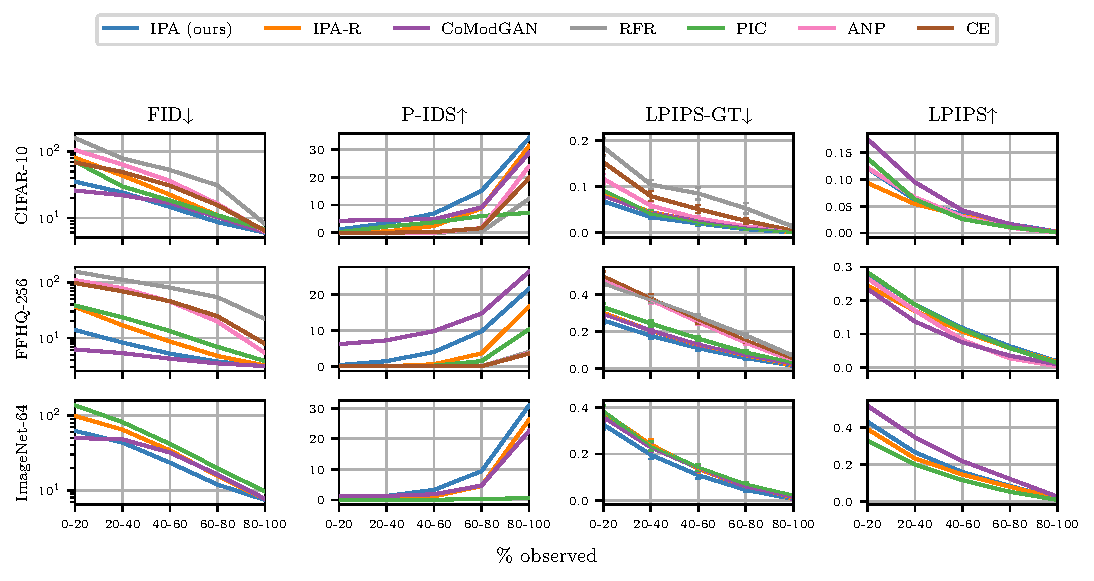
\includegraphics[width=\textwidth]{figs/cigcvae/extra-metrics}
  \caption{Additional comparisons between IPA and baselines on image completion, expanding on \cref{fig:cigcvae-metrics} with results on ImageNet-64 and the
    LPIPS diversity score.}
  \label{fig:cigcvae-extra-metrics}
\end{figure}

\begin{figure}
  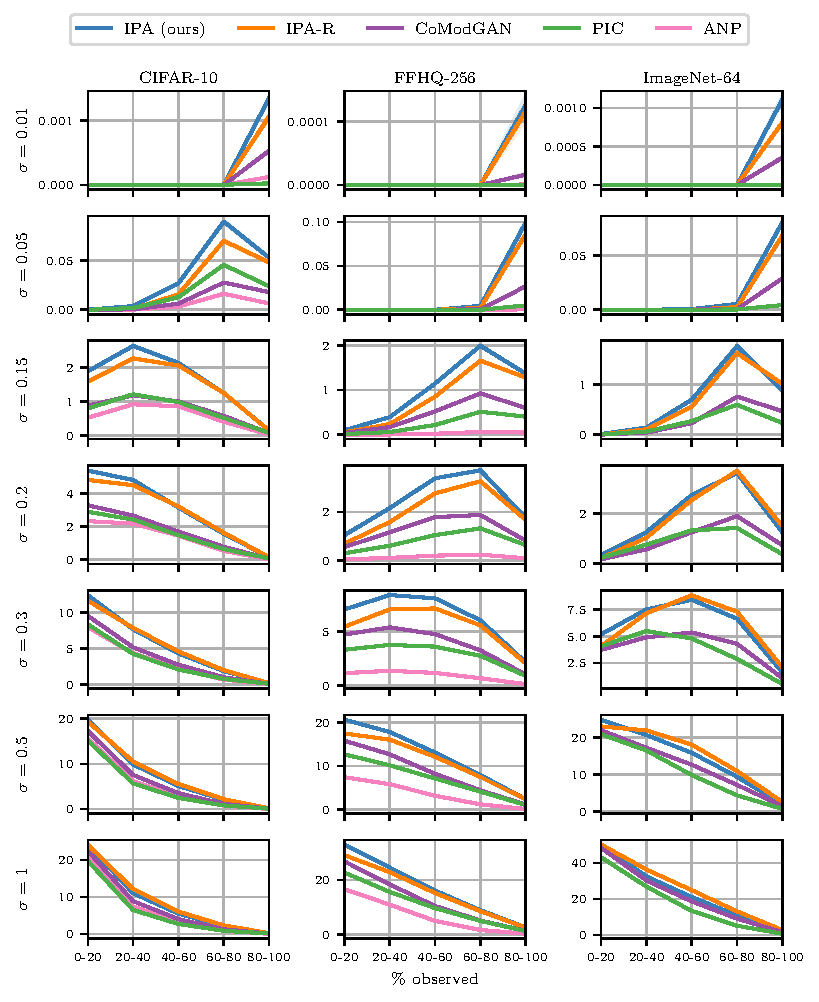
\includegraphics[width=0.95\textwidth]{figs/cigcvae/fwv_sigma}
  \caption{The faithfulness weighted variance metric for inpainting on CIFAR-10,
    FFHQ-256, and ImageNet-64, plotted for various values of its hyperparameter $\sigma$. IPA obtains the
    best performance on almost all datasets and values of $\sigma$, only being
    outperformed by IPA-R on CIFAR-10 with high values of $\sigma$. This
    indicates that IPA both assigns high probability density to the ground truth
    (and so performs well for small $\sigma$) and generates diverse samples (and
    so performs well for larger $\sigma$).}
  \label{fig:cigcvae-fwv}
\end{figure}



\section{Bayesian optimal experimental design} \label{sec:cigcvae-supp-boed}

\subsection{EIG estimators}  \label{sec:cigcvae-eig-estimator}

In this section, we expand on how our estimator for the expected information
gain differs from prior work~\citep{harvey2019near}. Repeating some relevant
definitions from the main text, $f_{\coord{}_1,\ldots,\coord{}_t}$ is a function which maps
from a full image to a sequence of observations of the image at locations
$\coord{}_1,\ldots,\coord{}_t$. When estimating the EIG at time step $t$, we will have already
observed a sequence of observations denoted $\rvy_{\coord{}_1,\ldots,\coord{}_{t-1}}$,
extracted from some latent image $\rvx$ as $f_{\coord{}_1,\ldots,\coord{}_{t-1}}(\rvx)$. We
use a CNN which outputs $g(v|f_{\coord{}_1,\ldots,\coord{}_t}(\rvx))$, an approximation of the
posterior over the latent variable of interest given a sequence of observations.
Following \citet{harvey2019near}, we will from now on refer to this as the
AVP-CNN (attentional variational posterior CNN).
%
Both our method and that of \citet{harvey2019near} sample image completions,
which we denote $\rvx^{(1)},\ldots,\rvx^{(N)}$, conditioned on
$\rvy_{\coord{}_1,\ldots,\coord{}_{t-1}}$. \citet{harvey2019near} do so by retrieving
images which roughly match the observed pixel values from a database. Although
completions from this are diverse, they can match the observed values poorly. We
therefore replace this stage with an image completion network trained using
IPA.

Given these components, \citet{harvey2019near} approximate the expected
information gain with
\begin{align}
  \label{eq:old-eig}
  \text{EIG}(\coord{}_t; \rvy_{\coord{}_1,\ldots,\coord{}_{t-1}}) &\approx \overbrace{\mathcal{H} \left[ g(\cdot|\rvy_{\coord{}_{1},\ldots,\coord{}_{t-1}}) \right]}^{\text{entropy after $t-1$ scans}} - \overbrace{\frac{1}{N} \sum_{n=1}^N  \mathcal{H} \left[ g(\cdot|f_{\coord{}_1,\ldots,\coord{}_t}(\rvx^{(n)})) \right]}^{\text{expected entropy after $t$ scans}}.
\end{align}
Since the prior entropy term of \cref{eq:old-eig} does not depend on $\coord{}_t$, it
can be neglected when choosing $\coord{}_t$ with BOED. As only the expected posterior
entropy then needs to be estimated and compared for various $\coord{}_t$, we will from
now on refer to this estimator with the acronym EPE (for `expected posterior
entropy').

We use a different estimator for the prior entropy. It becomes equivalent as $N
\rightarrow \infty$ if $g$ and the image completion method are perfect but, when
this is not the case, produces an estimate of the prior entropy with a
dependence on $\coord{}_t$. To repeat \cref{eq:new-eig}, this results in the following
estimator for the EIG:
\begin{align}
  \label{eq:new-eig-supp}
  \text{EIG}(\coord{}_t;& \rvy_{\coord{}_1,\ldots,\coord{}_{t-1}}) \approx \overbrace{\mathcal{H} \left[ \frac{1}{N} \sum_{n=1}^N g(\cdot|f_{\coord{}_1,\ldots,\coord{}_t}(\rvx^{(n)})) \right]}^{\text{entropy after $t-1$ scans}} - \overbrace{\frac{1}{N} \sum_{n=1}^N  \mathcal{H} \left[ g(\cdot|f_{\coord{}_1,\ldots,\coord{}_t}(\rvx^{(n)})) \right]}^{\text{expected entropy after $t$ scans}}.
\end{align}
While it is not immediately clear that this estimator is better than that in
\cref{eq:old-eig}, one useful property is that, like the true expected
information gain, it is guaranteed to be non-negative. This can be seen as
follows. First, note that the prior entropy term is the entropy of an
expectation (over $n \sim \text{Uniform}(1, N)$), and the expected posterior
entropy term swaps the order of the entropy and expectation. Since the mapping
from a distribution $g(\cdot)$ to its entropy $\mathcal{H}[g(\cdot)]$ is
strictly concave, Jensen's inequality is applicable. Invoking Jensen's
inequality shows that the prior entropy term must be greater than or equal to
the expected posterior entropy, and so the estimate of the EIG will be
non-negative. 
%In \cref{fig:cigcvae-boed-auroc-supp}, we compare the performance of this estimator (denoted EIG) and that in \cref{eq:old-eig} (EPE). We find that the estimator denoted EIG leads to significantly better classification performance.

Another view of our EIG estimator is as a variant of the inception
score~\citep{salimans2016improved} for the sampled images
$\rvx^{(1)},\ldots,\rvx^{(N)}$. The standard inception score is computed using
an image classifier trained on ImageNet~\citep{salimans2016improved}.
\Cref{eq:new-eig} is the inception score if this classifier is replaced with the
AVP-CNN acting on observations of each image at locations $\coord{}_1,\ldots,\coord{}_t$.

\begin{figure*}[t]
  \centering
  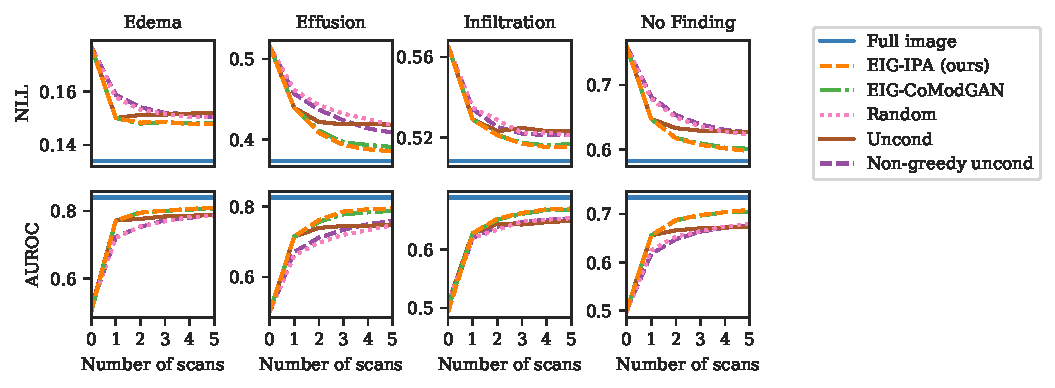
\includegraphics[width=\textwidth]{figs/cigcvae/boed-auroc-curve-supp}
  \caption{Evaluation and comparison of BOED systems for selecting scan locations, expanding on \cref{fig:cigcvae-boed} by additionally reporting negative
    log-likelihoods (top row) for the classification tasks. }
  \label{fig:cigcvae-boed-auroc-supp}
\end{figure*}

\begin{figure}[t]
  \centering
  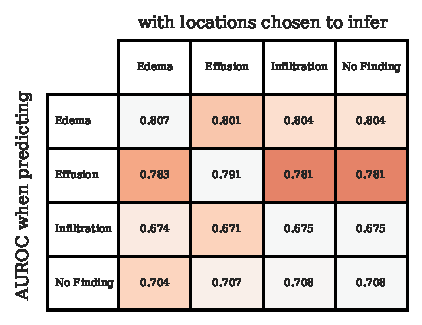
\includegraphics[width=0.6\textwidth]{figs/cigcvae/table-AUROC-boed}
  \caption{Evaluation of performance on each classification task when using scan locations chosen for a different classification task. We measure performance with the AUROC score. The intensity of the
    colour of each cell is proportional to the difference between its AUROC score and
    the greatest value in its row.}
  \label{fig:cigcvae-boed-correlations}
\end{figure}

\subsection{BOED baselines}
\paragraph{Random}
This baseline simply samples the scan location independently at each time step
from a uniform distribution over all valid locations.

\paragraph{Uncond}
This baseline ablates our estimator for the EIG (\cref{eq:new-eig}) by sampling
images $\rvx^{(1)},\ldots,\rvx^{(N)}$ from the training dataset (without
conditioning on $\rvy_{\coord{}_1,\ldots,\coord{}_{t-1}}$) instead of from IPA
(conditioned on $\rvy_{\coord{}_1,\ldots,\coord{}_{t-1}}$). That is, we use:
\begin{align}
  \label{eq:uncond}
  & \text{U}^{\text{uncond}}(\coord{}_t; \coord{}_1,\ldots,\coord{}_{t-1}) \\
  \nonumber & = \mathcal{H} \left[ \frac{1}{N} \sum_{n=1}^N g(\cdot|f_{\coord{}_1,\ldots,\coord{}_t}(\rvx^{(n)})) \right] - \frac{1}{N} \sum_{n=1}^N  \mathcal{H} \left[ g(\cdot|f_{\coord{}_1,\ldots,\coord{}_t}(\rvx^{(n)})) \right]
\end{align}
with $\rvx^{(1)},\ldots,\rvx^{(N)} \sim p(\rvx)$. The resulting choice of scan
location $\coord{}_t$ at each time step $t$ has no dependence on previous
observations $\rvy_{\coord{}_1,\ldots,\coord{}_{t-1}}$.

\paragraph{Non-greedy uncond}
When selecting scan locations that optimise the EIG, we select the scan location
at each time step greedily to optimise the EIG from the next scan. To do
otherwise (i.e.~maximise the EIG from multiple next scans) is intractable
because of the dependence of the EIG at each $t$ on previous observations
$\rvy_{\coord{}_1,\ldots,\coord{}_{t-1}}$. However, since the above `Uncond' baseline
selects each $\coord{}_t$ independently of what is observed at previous scans, we can
remove this greedy property. We do so by selecting all $\coord{}_1,\ldots,\coord{}_T$
simultaneously to maximise
\begin{align}
  \text{U}^{\text{non-greedy}}(\coord{}_1,&\ldots,\coord{}_T) = \mathcal{H} \left[ \frac{1}{N} \sum_{n=1}^N g(\cdot|f_{\emptyset}(\rvx^{(n)})) \right] - \frac{1}{N} \sum_{n=1}^N  \mathcal{H} \left[ g(\cdot|f_{\coord{}_1,\ldots,\coord{}_T}(\rvx^{(n)})) \right]
\end{align}
with $\rvx^{(1)},\ldots,\rvx^{(N)} \sim p(\rvx)$. Since the number of possible
values of $\coord{}_1,\ldots,\coord{}_T$ increases exponentially with $T$, it is not feasible
to search over all of them. We therefore optimise this sequence by
randomly sampling a set of such sequences, and choosing the best from this set.


\begin{figure*}[t]
  \centering
  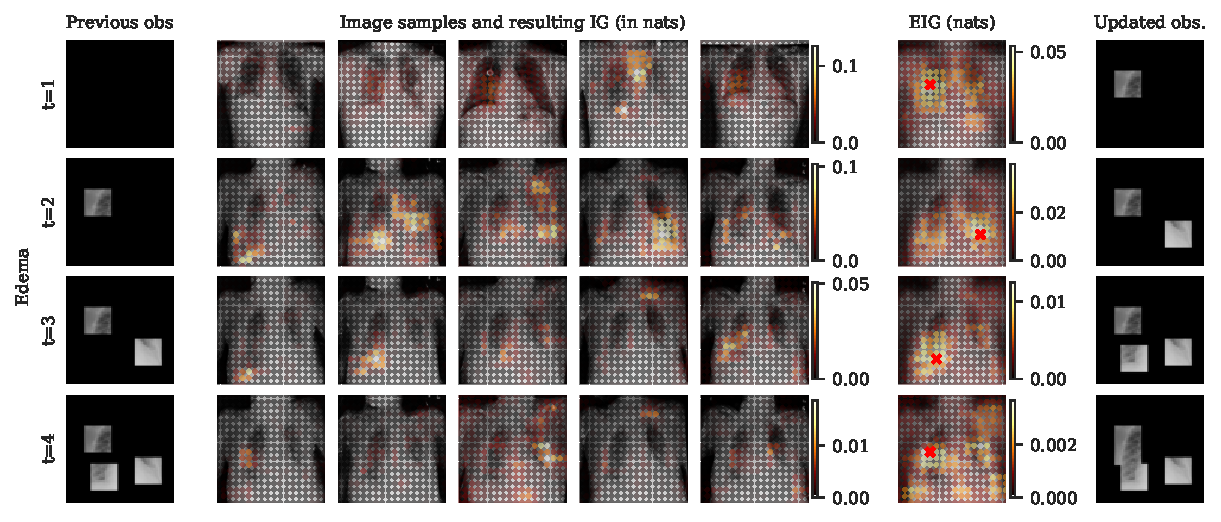
\includegraphics[width=0.98\textwidth]{figs/cigcvae/boed-visualisation-4960-compressed.pdf}
  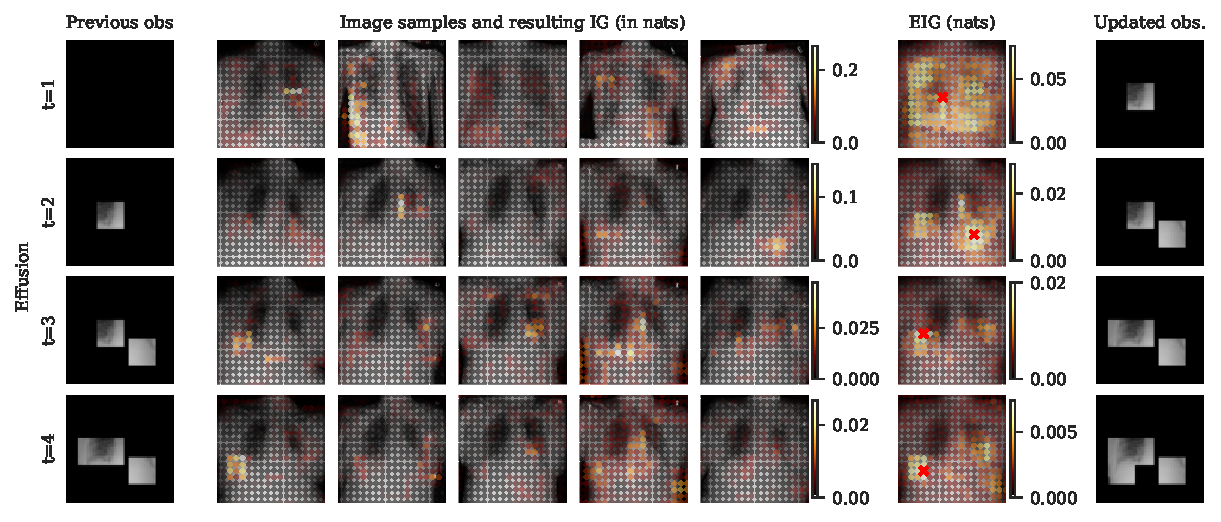
\includegraphics[width=0.98\textwidth]{figs/cigcvae/boed-visualisation-4970-compressed.pdf}
  \caption{Visualisations of the selection of scan locations with BOED. On the top, the task is to detect
    `Edema'. In the middle, we aim to detect `Effusion' in a different patient.
    Four scan locations are
    selected for each. The left column shows the observations made before
    selecting each scan location. The next five columns show five of the $N=10$
    sampled image completions conditioned on these observations. Each is
    overlaid with the information gain predicted after scanning any location.
    The second column from the left shows the expected information gain at each
    location, given by averaging the information gains arising from each sampled
    image completion. A red cross marks the maximum. The final column shows the
    updated observations after scanning the location which maximises the
    expected information gain. We show one more example in \cref{fig:cigcvae-extra-xray-boed-extra}.}
  \label{fig:cigcvae-extra-xray-boed}
\end{figure*}

\begin{figure*}[t]
  \centering
  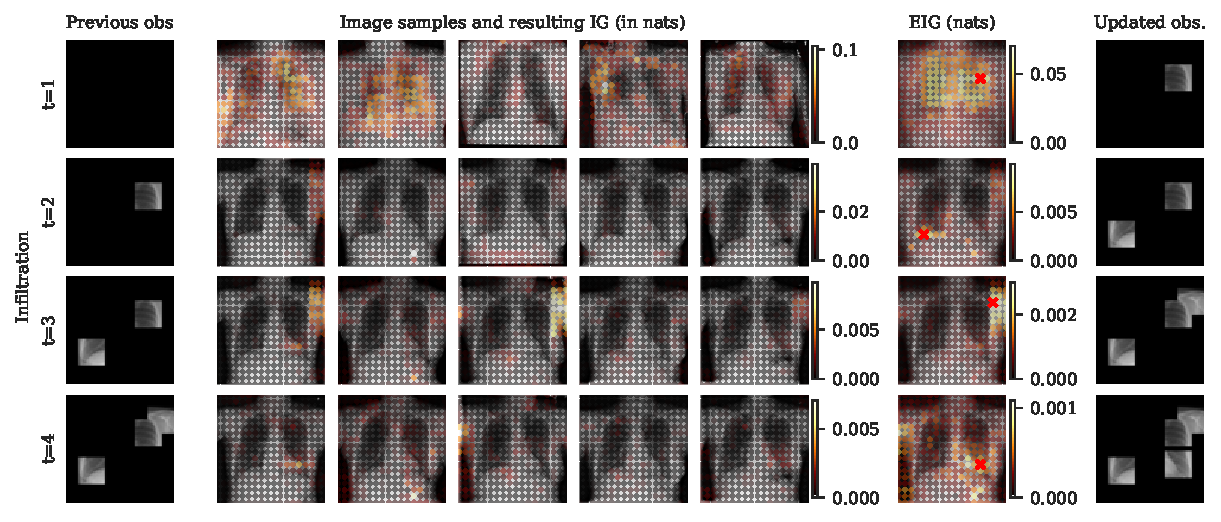
\includegraphics[width=\textwidth]{figs/cigcvae/boed-visualisation-4980-compressed.pdf}
  \caption{Another visualisation of the selection of scan locations with BOED similar to \cref{fig:cigcvae-extra-xray-boed}, where the task is to detect the presence of `Infiltration'.}
\label{fig:cigcvae-extra-xray-boed-extra}
\end{figure*}

\subsection{Additional BOED results} \label{supp:cigcvae-boed-results}
\Cref{fig:cigcvae-boed-auroc-supp} shows additional results from classification with
sequences chosen by BOED and our baselines. In particular, we report negative
log-likelihoods for the class labels as well as the AUROC scores. We see that
the negative log-likelihood sometimes increases as more scans are taken,
indicating that the classifier used is not perfectly trained. 
% Interestingly,
% this only happens when glimpses are chosen with the EPE estimator of
% \citet{harvey2019near}. This may be because the EPE estimator has a tendency to
% select locations which cause the classifier to be overconfident (and thus
% produce artificially low posterior entropies). With the EIG estimator, and the
% baselines, this issue is not observed.

To illustrate that the scan locations chosen by BOED are task-dependent,
in \cref{fig:cigcvae-boed-correlations} we show the results from using scan locations chosen
for one classification task (i.e.~diagnosing a particular disease) to perform a
different classification task. Each row shows the results for a particular task,
with each column showing results when scan locations are chosen based on a
particular task. As expected, the highest (or at least joint-highest) AUROC
score in each row occurs on the diagonal, when the classification task and
choice of scan locations are aligned. Away from the diagonal, the scores are
only slightly lower, perhaps reflecting that there is a large overlap between
the relevant areas for these tasks.

\Cref{fig:cigcvae-extra-xray-boed} shows additional visualisations of the Bayesian
experimental design process for different test images, adding to the one shown
in the main paper. The `information gains' shown for a particular $\rvx^*$
(sampled conditioned on observations $\rvy_{\coord{}_1,\ldots,\coord{}_{t-1}}$) are
computed as the following KL divergence:
% EIG but the `expected
% entropy after $t$ scans' term is replaced by the entropy given a particular
% sampled $\rvx^*$. That is,
\begin{align}
  \label{eq:ig}
                                                   \text{IG}(\rvx^*, \coord{}_t; \rvy_{\coord{}_1,\ldots,\coord{}_{t-1}}) \approx \kl[\Bigg]{g(\cdot|f_{\coord{}_1,\ldots,\coord{}_t}(\rvx^*))}{\frac{1}{N} \sum_{n=1}^N g(\cdot|f_{\coord{}_1,\ldots,\coord{}_t}(\rvx^{(n)}))}.
\end{align}
Crucially, averaging information gains computed with $\rvx^*=\rvx^{(1)}$ to
$\rvx^{(N)}$ gives the estimate of the EIG presented in \cref{eq:new-eig}.

\subsection{BOED experimental details}
The AVP-CNN, $g$, is trained to map from masked images, $\rvy$, to
distributions over the class labels. Each image in the Chest X-ray 14 dataset
has labels indicating the presence or absence of each of 14 pathologies. We
train $g$ to produce 15 outputs: an estimated probability of the presence or
absence of each of the 14 conditions individually; and an additional estimate of
the probability that any (one or more) of these conditions is present. We train
$g$ to estimate these using a cross-entropy loss. Masked images are sampled
using almost the same mask distribution as for training the image completion
networks (described in \cref{sec:cigcvae-experiments}); the only difference is that
patches now have 25\% rather than 35\% of the image width, to match the
observations we use in the experiments with BOED. We use an AVP-CNN pretrained
on ImageNet and then trained on Chest X-ray 14 for 32\,000 iterations with a
batch size of 32 and learning rate $1\times10^{-5}$. We train IPA as described
in \cref{supp:cigcvae-exp-details}.

We select each scan location by evaluating \cref{eq:new-eig} at every point in
an evenly-spaced $17\times17$ grid over the image, and choosing the maximum. We
evaluate the EIG with $N=10$ sampled image completions. This is repeated to
select the scan location for each $t=1,\ldots,5$ (with the sampled images
conditioned on observations up to $t-1$ at each stage). Where applicable, we use
the same trained networks and hyperparameters for the baselines. For the
`non-greedy uncond' baseline, we select a scan location sequence by choosing the
best of 289 sampled sequences. This number was chosen to match the number of
locations in the $17\times17$ grid that the other methods search over at each
time step. The results reported in \cref{fig:cigcvae-boed,fig:cigcvae-boed-auroc-supp} were
computed on a randomly-sampled 5000 image subset of the Chest X-ray 14 test set.


\section{Out-of-distribution detection} \label{supp:cigcvae-ood} A major advantage of
likelihood-based models is the possibility to use them to detect when an input
is dissimilar to the training data (out-of-distribution, or OOD). Since a
learned model is likely to perform poorly on such inputs, it is important for
deployed systems to be able to recognise them and this has been the focus of a
substantial body of
work~\citep{ren2019likelihood,hendrycks2016baseline,xiao2020likelihood,havtorn2021hierarchical}.
The task we consider is detecting whether a partially observed image (e.g.~the
input to an image completion system) is OOD.


\begin{figure}[t]
    \footnotesize
  \centering
  \begin{minipage}{0.41\textwidth}

    \centering
    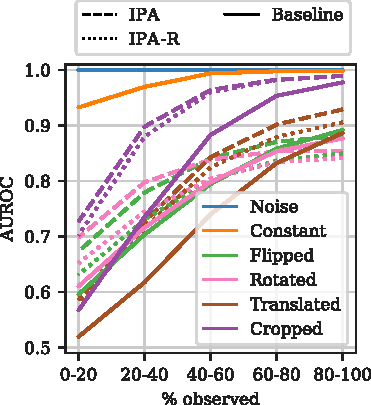
\includegraphics[scale=.8]{figs/cigcvae/ood-ffhq}

  \end{minipage}
  \begin{minipage}{.58\textwidth}

%  \caption{AUROC scores for OOD detection. Higher is better.}
  \begin{tabular}{lccccc}
    \toprule
    ID & \multicolumn{5}{c}{CIFAR-10}  \\
    \cmidrule(r){2-6}
    OOD & Noise & Const. & Flip & Rot. & SVHN \\
    \midrule
    IPA      & \textbf{.995} & \textbf{.949} & \underline{.552} & \underline{.594} & \textbf{.753}    \\
    IPA-R    & .987         & \underline{.921}                  & \textbf{.635}    & \textbf{.619}    & \underline{.686} \\
    Baseline  & \underline{.993} & .909 & .543             & .536             & .556             \\
    \bottomrule
  \end{tabular}
  \newline
  \vspace*{.1cm}
  \newline
  \begin{tabular}{lcccccc}
    \toprule
    ID & \multicolumn{5}{c}{FFHQ-256}  \\
    \cmidrule(r){2-6}
    OOD         & Noise & Const. & Flip & Rot. & ~Crop~ \\
    \midrule
    IPA         & \textbf{1.00} & \textbf{1.00} & \textbf{.809}    & \textbf{.808}    & \textbf{.912}    \\
    IPA-R       & \textbf{1.00} & \textbf{1.00} & \underline{.770} & \underline{.775} & \underline{.902} \\
    Baseline     & \textbf{1.00} & 0.98  & .769 & .771             & .823             \\
    \bottomrule
  \end{tabular}

\end{minipage}%
\caption{Out-of-distribution detection on partially-observed images. On the left, we show AUROC scores
  on FFHQ-256 computed separately for masks from varying distributions. On the
  right we report, for both CIFAR-10 and FFHQ-256, the average of these scores
  over all mask distributions.}
\label{fig:cigcvae-ood-results}
% \vspace{-.5cm}
\end{figure}

OOD-detection using probabilistic models is theoretically appealing and robust,
since no assumptions need to be made about the OOD
data~\citep{xiao2020likelihood,havtorn2021hierarchical}. Such OOD-detection
metrics commonly have the following interface: they take as input a
probabilistic model (e.g.~a VAE) and a data point, and output a scalar value.
The greater the value of this scalar, the more likely it is that the data point
is within the distribution of the generative model. One intuitive metric is
simply the log-likelihood of the data point under the model. This can work
poorly in practice, however, and it has been found that learned models sometimes
assign higher likelihood to out-of-distribution data than to in-distribution
data~\citep{nalisnick2018deep}. Several alternative OOD-detection metrics have
been proposed specifically for
VAEs~\citep{xiao2020likelihood,havtorn2021hierarchical}. To use them, we note
that we can use networks trained with either IPA or IPA-R to lower-bound the
likelihood of a partially-observed image. Specifically, this lower-bound is the
reverse KL objective in \cref{eq:reverse-obj}. After conducting preliminary
experiments using the VD-VAE with several OOD-detection
metrics~\citep{xiao2020likelihood,havtorn2021hierarchical}, we found that
\begin{figure}[t]
  \centering
  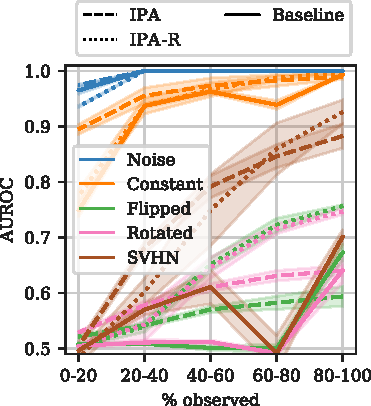
\includegraphics[scale=1]{figs/cigcvae/ood-supplementary}
  \caption{An evaluation of our method for out-of-distribution detection on partially-observed images. We show the AUROC as a function of the proportion of image which is observed. The model is trained on CIFAR-10 and we plot performance for a variety of types of out-of-distribution image.. }
  \label{fig:cigcvae-ood-supplementary}
\end{figure}
improved performance could be obtained (for OOD-detection of both partially- and
fully-observed images) using the ``temperature gradient'' metric described
further in \cref{supp:cigcvae-temp-grad} below.
%
It is efficient to compute, requiring the VAE to be run just once and gradients
computed.

As a baseline, we complete the partially observed image with our best performing
baseline image completion method, CoModGAN, and perform OOD-detection on the
result (using the ``temperature gradient'' metric on an unconditional VD-VAE).
\Cref{fig:cigcvae-ood-results} shows our results on CIFAR-10 and FFHQ-256. We test
various types of OOD data: \textbf{Noise} samples each pixel value independently
from a uniform distribution; \textbf{Constant} uniformly samples a single colour
for the entire image; \textbf{Flip} vertically flips an in-distribution (ID)
image; \textbf{Rotate} rotates an ID image by 90$^{\circ}$; \textbf{Crop}
upsamples an ID image by a factor of 1.5 and then crops to the original size.
\textbf{SVHN} is the Street View House Number dataset~\citep{netzer2011reading}.
With 80-100\% of the image observed, we obtain better AUROCs than similar
methods applied to the full image. In particular, on CIFAR-10 vs SVHN, we
outperform both \citet{xiao2020likelihood} and \citet{havtorn2021hierarchical},
albeit with a larger VAE architecture. Using IPA for OOD-detection results in
performance that degrades gracefully as less of the image is observed. There are
therefore particularly large benefits over the baseline when only 0-20\% or
20-40\% of the image is observed.

\Cref{fig:cigcvae-ood-supplementary} shows a breakdown of the AUROC scores for each mask
distribution on CIFAR-10, similar to that shown for FFHQ-256 in
\cref{fig:cigcvae-ood-results}. Error bars are standard deviations computed with 3 runs,
with the unconditional VD-VAE and IPA/IPA-R retrained each time.



\subsection{Out-of-distribution detection with temperature gradients} \label{supp:cigcvae-temp-grad}


We conducted preliminary experiments with several techniques for OOD-detection
with VAEs, applying each to the VD-VAE architecture. Using the likelihood-regret
technique~\citep{xiao2020likelihood} with the VD-VAE is computationally costly
(as it involves optimising neural network parameters), and we obtained results
on CIFAR-10 considerably worse than those produced by the smaller VAE
architecture with which it was introduced. We also implemented the
log-likelihood ratio metric \citep{havtorn2021hierarchical} for the VD-VAE, but
did not find any hyperparameter configurations with which it was consistently
better than random guessing across different tasks.

We therefore introduce a metric which we found to work well with the VD-VAE. It
is based on a common heuristic to make a VAE produce more regular samples:
reducing the variance of the prior over its latent
variables~\citep{vahdat2020nvae}. If $\mathbf{t}$ is a vector containing the
temperature $\mathbf{t}_l$ for each layer $l$, then doing so corresponds to
modifying the prior $p_\theta(\rvz)$ so that the Gaussian distribution over each
group of latent variables is scaled by the corresponding temperature:
\begin{equation}
  p_\theta(\rvz; \mathbf{t}) = \prod_{l=1}^L  \frac{1}{C(\mathbf{t}_l, \rvz_{<l})} p_\theta(\rvz_l|\rvz_{<l})^{\frac{1}{\mathbf{t}^2_l}}
\end{equation}
where $C(\mathbf{t}_l, \rvz_{<l})$ is a normalisation constant. In practice, since
$p_\theta(\rvz_l|\rvz_{<l})$ is a Gaussian distribution, this scaling corresponds to
simply multiplying the standard deviation by $\mathbf{t}_l$.

We can lower-bound the corresponding marginal likelihood $p_\theta(\rvy;
\mathbf{t})$ using the partial encoder similarly to the training objective in
\cref{eq:reverse-obj}:
\begin{align}
  \EX_{\pdata (\rvy)} \left[ \log p_\theta(\rvy; \mathbf{t}) \right] \geq \EX_{\pdata (\rvy)}\EX_{p_\psi(\rvz|\rvy)} \left[ \log\frac{p_\theta(\rvz; \mathbf{t})p_\theta(\rvy|\rvz)}{p_\psi(\rvz|\rvy)} \right] .
\end{align}
We hypothesise that OOD examples will usually either be excessively regular, and
therefore have a higher marginal likelihood for $t<1$, or excessively irregular,
and therefore have a higher likelihood for $t>1$. In-distribution (ID) examples,
on the other hand, should have the highest marginal likelihood for $t\approx 1$.
A useful feature to distinguish between ID and OOD examples is therefore likely
to be the gradient $\frac{\partial}{\partial\mathbf{t}}p(\rvy;
\mathbf{t})\lvert_{\mathbf{t}=\mathbf{1}}$, which we can approximate with the
gradient w.r.t. $\mathbf{t}$ of the lower-bound above. We fit a multivariate
Gaussian to 5000 samples of
$\frac{\partial}{\partial\mathbf{t}}p(\rvy^{(i)};
\mathbf{t})\lvert_{\mathbf{t}=\mathbf{1}}$ with $\rvy^{(i)}$ sampled from
the training data with the training mask distribution. To obtain a score for how
in-distribution a new example $\rvy$ is, we compute the probability density
of $\frac{\partial}{\partial\mathbf{t}}p(\rvy;
\mathbf{t})\lvert_{\mathbf{t}=\mathbf{1}}$ under this multivariate Gaussian. The
greater this score, the more likely it is that an example is in-distribution. We
call this the ``temperature-gradient'' metric.

\subsection{OOD detection details} We compute the AUROC scores presented in
\cref{fig:cigcvae-ood-results} using the 5000 image test set for CIFAR-10 and its
OOD-transformations; a 5000 images subset of the SVHN test set; and the 7000
image test set for FFHQ-256. We use 5000 samples of $32\times32$ `Noise' and
`Constant' images when comparing against CIFAR-10, and 200 samples at
$256\times256$ resolution when comparing against FFHQ-256. We also present results for the `Translated' transformation in
\cref{fig:cigcvae-ood-results} for FFHQ-256. This transformation takes a crop with 90\%
of the image size from one of the four corners and then rescales it to the
original size. The result is thus slightly translated so that e.g.~the eyes of
an FFHQ image are no longer aligned. It is not shown in our results table due to
space constraints.


\section{Lack of semantic diversity in CoModGAN} \label{supp:cigcvae-comodgan-failure}
In this section we demonstrate the some failure cases of CoModGAN in which it
fails to produce semantically diverse images. We suspect that this behaviour of
CoModGAN contributes to its poor performance on the LPIPS-GT metric.
\Cref{fig:cigcvae-comodgan-failure} shows a few examples of partial images for which
CoModGAN struggles to generate semantically diverse images. Compare these
results with IPA's results reported in \cref{fig:cigcvae-comodgan-failure-aipo},
showing a wide range of completions for all the partial images.

\newcommand{\cmgfailureimgheight}{0.8cm}

\begin{figure*}[t]
  \centering
  \begin{subfigure}[t]{0.14\textwidth}
    \centering
    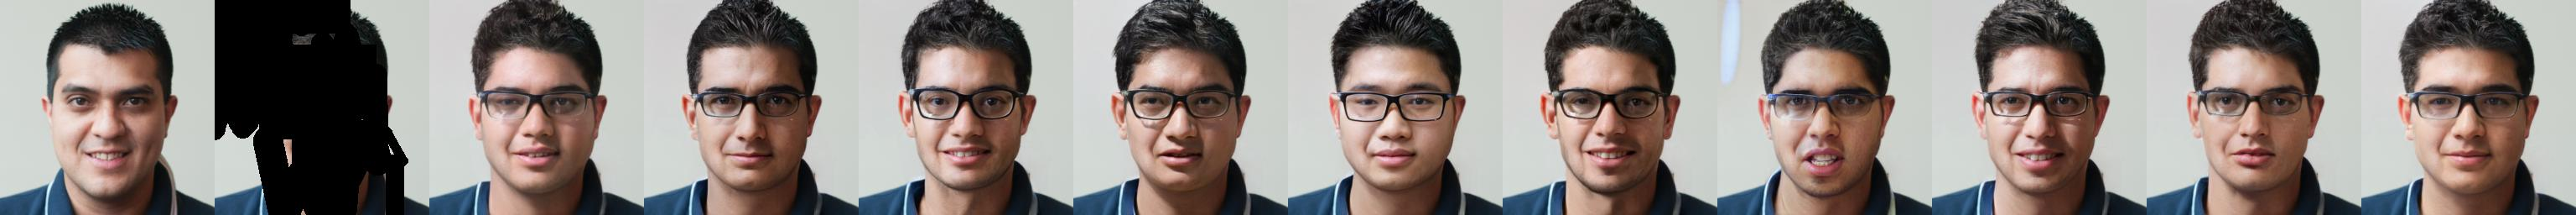
\includegraphics[trim=0px 0px 2560px 0px, clip, height=\cmgfailureimgheight]{figs/cigcvae/co_mod_gan_failure/co_mod_gan_0_3_2.jpg}
    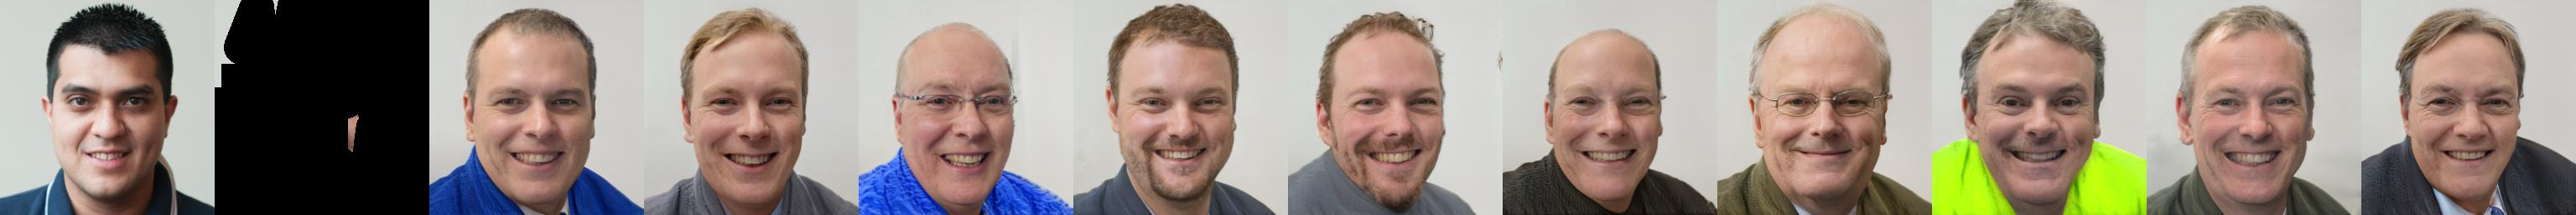
\includegraphics[trim=0px 0px 2560px 0px, clip, height=\cmgfailureimgheight]{figs/cigcvae/co_mod_gan_failure/co_mod_gan_0_4_2.jpg}
    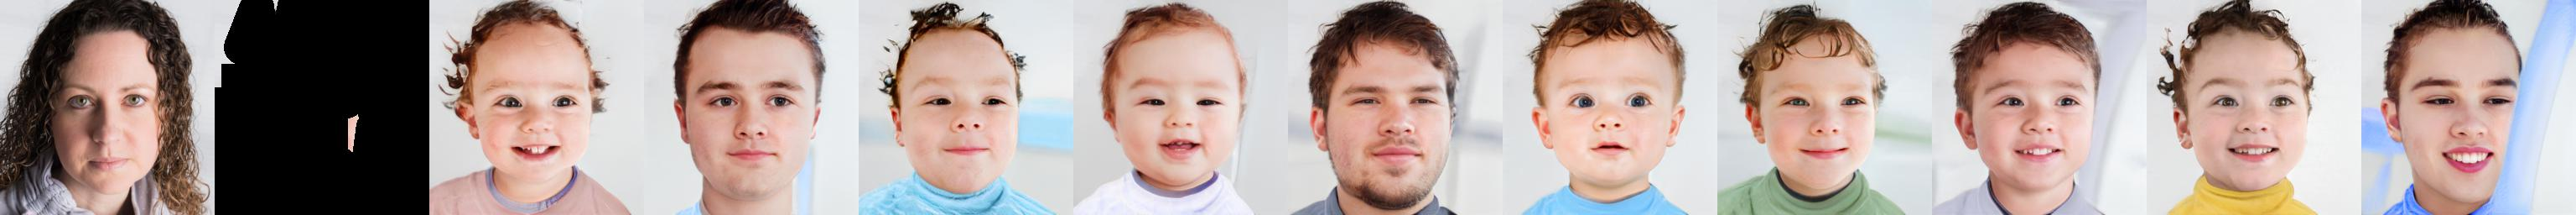
\includegraphics[trim=0px 0px 2560px 0px, clip, height=\cmgfailureimgheight]{figs/cigcvae/co_mod_gan_failure/co_mod_gan_1_4_2.jpg}
    \includegraphics[trim=0px 0px 2560px 0px, clip, height=\cmgfailureimgheight]{figs/cigcvae/co_mod_gan_failure/co_mod_gan_56_4_12.jpg}
    \caption{\scriptsize $\rvx, \rvy$}
  \end{subfigure}
  \begin{subfigure}[t]{0.73\textwidth}
    \centering
    \includegraphics[trim=512px 0px 0px 0px, clip, height=\cmgfailureimgheight]{figs/cigcvae/co_mod_gan_failure/co_mod_gan_0_3_2.jpg}
    \includegraphics[trim=512px 0px 0px 0px, clip, height=\cmgfailureimgheight]{figs/cigcvae/co_mod_gan_failure/co_mod_gan_0_4_2.jpg}
    \includegraphics[trim=512px 0px 0px 0px, clip, height=\cmgfailureimgheight]{figs/cigcvae/co_mod_gan_failure/co_mod_gan_1_4_2.jpg}
    \includegraphics[trim=512px 0px 0px 0px, clip, height=\cmgfailureimgheight]{figs/cigcvae/co_mod_gan_failure/co_mod_gan_56_4_12.jpg}
    \caption{\scriptsize Sampled completions}
  \end{subfigure}
  \begin{subfigure}[t]{0.1\textwidth}
    \centering
    \includegraphics[height=\cmgfailureimgheight]{figs/cigcvae/co_mod_gan_failure/avg_co_mod_gan_0_3_2.jpg}
    \includegraphics[height=\cmgfailureimgheight]{figs/cigcvae/co_mod_gan_failure/avg_co_mod_gan_0_4_2.jpg}
    \includegraphics[height=\cmgfailureimgheight]{figs/cigcvae/co_mod_gan_failure/avg_co_mod_gan_1_4_2.jpg}
    \includegraphics[height=\cmgfailureimgheight]{figs/cigcvae/co_mod_gan_failure/avg_co_mod_gan_56_4_12.jpg}
    \caption{\scriptsize Mean}
  \end{subfigure}
  %%%%%%%%%%%%%%%%%%%%%%
  \caption{Examples of image completion tasks on which CoModGAN fails to model the semantic diversity in the distribution of possible completions. Panel
    (a) shows the true image and the masked version on which the completions are
    conditioned. Panel (b) shows 10 completions sampled randomly from the
    CoModGAN model. Panel (c) shows the mean image computed from 100 sampled
    completions. On each row, the completions are mostly semantically similar to
    eachother yet different from the ground truth image, indicating that they
    are not faithfully representing the true posterior. This behaviour can be
    contrasted with that of IPA in \cref{fig:cigcvae-comodgan-failure-aipo}.}
  \label{fig:cigcvae-comodgan-failure}
  \vspace{.5cm}
  \begin{subfigure}[t]{0.14\textwidth}
    \centering
    \includegraphics[trim=0px 0px 2560px 0px, clip, height=\cmgfailureimgheight]{figs/cigcvae/co_mod_gan_failure/aipo_0_3_2.jpg}
    \includegraphics[trim=0px 0px 2560px 0px, clip, height=\cmgfailureimgheight]{figs/cigcvae/co_mod_gan_failure/aipo_0_4_2.jpg}
    \includegraphics[trim=0px 0px 2560px 0px, clip, height=\cmgfailureimgheight]{figs/cigcvae/co_mod_gan_failure/aipo_1_4_2.jpg}
    \includegraphics[trim=0px 0px 2560px 0px, clip, height=\cmgfailureimgheight]{figs/cigcvae/co_mod_gan_failure/aipo_56_4_12.jpg}
    \caption{\scriptsize $\rvx, \rvy$}
  \end{subfigure}
  \begin{subfigure}[t]{0.73\textwidth}
    \centering
    \includegraphics[trim=512px 0px 0px 0px, clip, height=\cmgfailureimgheight]{figs/cigcvae/co_mod_gan_failure/aipo_0_3_2.jpg}
    \includegraphics[trim=512px 0px 0px 0px, clip, height=\cmgfailureimgheight]{figs/cigcvae/co_mod_gan_failure/aipo_0_4_2.jpg}
    \includegraphics[trim=512px 0px 0px 0px, clip, height=\cmgfailureimgheight]{figs/cigcvae/co_mod_gan_failure/aipo_1_4_2.jpg}
    \includegraphics[trim=512px 0px 0px 0px, clip, height=\cmgfailureimgheight]{figs/cigcvae/co_mod_gan_failure/aipo_56_4_12.jpg}
    \caption{\scriptsize Sampled completions}
  \end{subfigure}
  \begin{subfigure}[t]{0.1\textwidth}
    \centering
    \includegraphics[height=\cmgfailureimgheight]{figs/cigcvae/co_mod_gan_failure/avg_aipo_0_3_2.jpg}
    \includegraphics[height=\cmgfailureimgheight]{figs/cigcvae/co_mod_gan_failure/avg_aipo_0_4_2.jpg}
    \includegraphics[height=\cmgfailureimgheight]{figs/cigcvae/co_mod_gan_failure/avg_aipo_1_4_2.jpg}
    \includegraphics[height=\cmgfailureimgheight]{figs/cigcvae/co_mod_gan_failure/avg_aipo_56_4_12.jpg}
    \caption{\scriptsize Mean}
  \end{subfigure}
  %%%%%%%%%%%%%%%%%%%%%%
  \caption{Examples completions from our IPA model on the tasks in which CoModGAN lacked semantic diversity (see
    \cref{fig:cigcvae-comodgan-failure}). These samples from IPA provide a much better
    representation of the inherent uncertainty in the image given the
    observations. We did not find any $(\rvx, \rvy)$ pairs on which the IPA
    model failed in the same way as CoModGAN in \cref{fig:cigcvae-comodgan-failure}. }
  \label{fig:cigcvae-comodgan-failure-aipo}
\end{figure*}

\section{Image samples}\label{supp:cigcvae-image-samples}


\Cref{fig:cigcvae-cifar-samples-0,fig:cigcvae-imagenet-samples,fig:cigcvae-ffhq-samples,fig:cigcvae-bags-samples,fig:cigcvae-shoes-samples,fig:cigcvae-xray-samples}
on the following pages show conditionally generated images for all datasets we have
experimented with, from both IPA and our baselines. It is apparent from the
image samples, particularly when the number of observed pixels is small, that
IPA-R has less sample diversity than IPA, which can be explained by the
mode-seeking behaviour of the reverse-KL and subsequent under-estimation of
posterior uncertainty \citep{minka2005divergence}. Finally, we note a flaw with
some of the completions produced by IPA: a lack of bilateral symmetry in
FFHQ-256 samples. Again, this is most apparent when few pixels are observed.
This issue can be seen in unconditional samples from the underlying VAEs as well
(see the samples reported by \citet{child2020very}). Therefore, it is likely
that any future advances in image modelling with VAEs could be integrated to
improve this aspect of the results.

\newcommand{\qualimgheight}{4cm} 
\newcommand{\qualcaption}[1]{Sampled
  completions from each method for #1 image. Panels (a), (d) and (h) all show
  the true image and the masked image on which the samples in each row are
  conditioned. Panels (b) and (c) show completions from IPA and IPA-R. (g) and
  (k) show the single deterministic completion produced by CE and RFR
  respectively. Each of the remaining panels show five completions for the
  stochastic baselines.} \newcommand{\freeformimgheight}{0.8cm}


% CIFAR samples -------------------------------------------------------------------------------------------------------------
\newcommand{\cifarimgheight}{1.2cm}
\newcommand{\clipby}{20}
  \begin{figure*}[t]
    \centering
    \begin{subfigure}[t]{0.11\textwidth}
      \centering
      \includegraphics[height=\cifarimgheight]{figs/cigcvae/image-samples/cifar10/freeform_aipo_0_gt_masked}
      \includegraphics[height=\cifarimgheight]{figs/cigcvae/image-samples/cifar10/freeform_aipo_1_gt_masked}
      \includegraphics[height=\cifarimgheight]{figs/cigcvae/image-samples/cifar10/freeform_aipo_3_gt_masked}
      \caption{\scriptsize $\rvx, \rvy$}
    \end{subfigure}
    \begin{subfigure}[t]{0.17\textwidth}
      \centering
      \includegraphics[height=\cifarimgheight]{figs/cigcvae/image-samples/cifar10/freeform_aipo_0_t=0.85_samples}
      \includegraphics[height=\cifarimgheight]{figs/cigcvae/image-samples/cifar10/freeform_aipo_1_t=0.85_samples}
      \includegraphics[height=\cifarimgheight]{figs/cigcvae/image-samples/cifar10/freeform_aipo_3_t=0.85_samples}
      \caption{\scriptsize IPA, $t=0.85$}
    \end{subfigure}
    \begin{subfigure}[t]{0.17\textwidth}
      \centering
      \includegraphics[height=\cifarimgheight]{figs/cigcvae/image-samples/cifar10/freeform_aipo_0_samples}
      \includegraphics[height=\cifarimgheight]{figs/cigcvae/image-samples/cifar10/freeform_aipo_1_samples}
      \includegraphics[height=\cifarimgheight]{figs/cigcvae/image-samples/cifar10/freeform_aipo_3_samples}
      \caption{\scriptsize IPA}
    \end{subfigure}
    \begin{subfigure}[t]{0.17\textwidth}
      \centering
      \includegraphics[height=\cifarimgheight]{figs/cigcvae/image-samples/cifar10/freeform_aipo_0_imagenet_samples}
      \includegraphics[height=\cifarimgheight]{figs/cigcvae/image-samples/cifar10/freeform_aipo_1_imagenet_samples}
      \includegraphics[height=\cifarimgheight]{figs/cigcvae/image-samples/cifar10/freeform_aipo_3_imagenet_samples}
      \caption{\scriptsize \shortstack{ IPA from \\ ImageNet}}
    \end{subfigure}
    \begin{subfigure}[t]{0.17\textwidth}
      \centering
      \includegraphics[height=\cifarimgheight]{figs/cigcvae/image-samples/cifar10/freeform_aipo_0_scratch_samples}
      \includegraphics[height=\cifarimgheight]{figs/cigcvae/image-samples/cifar10/freeform_aipo_1_scratch_samples}
      \includegraphics[height=\cifarimgheight]{figs/cigcvae/image-samples/cifar10/freeform_aipo_3_scratch_samples}
      \caption{\scriptsize \shortstack{ IPA from \\ scratch}}
    \end{subfigure}
    \begin{subfigure}[t]{0.17\textwidth}
      \centering
      \includegraphics[height=\cifarimgheight]{figs/cigcvae/image-samples/cifar10/freeform_aipo-r_0_samples}
      \includegraphics[height=\cifarimgheight]{figs/cigcvae/image-samples/cifar10/freeform_aipo-r_1_samples}
      \includegraphics[height=\cifarimgheight]{figs/cigcvae/image-samples/cifar10/freeform_aipo-r_3_samples}
      \caption{\scriptsize IPA-R}
    \end{subfigure}
    %%%%%%%%%%%%%%%%%%%%%%
    \begin{subfigure}[t]{0.11\textwidth}
      \centering
      \includegraphics[height=\cifarimgheight]{figs/cigcvae/image-samples/cifar10/freeform_aipo_0_gt_masked}
      \includegraphics[height=\cifarimgheight]{figs/cigcvae/image-samples/cifar10/freeform_aipo_1_gt_masked}
      \includegraphics[height=\cifarimgheight]{figs/cigcvae/image-samples/cifar10/freeform_aipo_3_gt_masked}
      \caption*{\scriptsize $\rvx, \rvy$}
    \end{subfigure}
    \begin{subfigure}[t]{0.17\textwidth}
      \centering
      \includegraphics[height=\cifarimgheight]{figs/cigcvae/image-samples/cifar10/freeform_co_mod_gan_0_samples}
      \includegraphics[height=\cifarimgheight]{figs/cigcvae/image-samples/cifar10/freeform_co_mod_gan_1_samples}
      \includegraphics[height=\cifarimgheight]{figs/cigcvae/image-samples/cifar10/freeform_co_mod_gan_3_samples}
      \caption{\scriptsize CoModGAN}
    \end{subfigure}
    \begin{subfigure}[t]{0.17\textwidth}
      \centering
      \includegraphics[height=\cifarimgheight]{figs/cigcvae/image-samples/cifar10/freeform_pic_0_samples}
      \includegraphics[height=\cifarimgheight]{figs/cigcvae/image-samples/cifar10/freeform_pic_1_samples}
      \includegraphics[height=\cifarimgheight]{figs/cigcvae/image-samples/cifar10/freeform_pic_3_samples}
      \caption{\scriptsize PIC}
    \end{subfigure}
    \begin{subfigure}[t]{0.17\textwidth}
      \centering
      \includegraphics[height=\cifarimgheight]{figs/cigcvae/image-samples/cifar10/freeform_anp_0_samples}
      \includegraphics[height=\cifarimgheight]{figs/cigcvae/image-samples/cifar10/freeform_anp_1_samples}
      \includegraphics[height=\cifarimgheight]{figs/cigcvae/image-samples/cifar10/freeform_anp_3_samples}
      \caption{\scriptsize ANP}
    \end{subfigure}
    \begin{subfigure}[t]{0.17\textwidth}
      \centering
      \includegraphics[height=\cifarimgheight]{figs/cigcvae/image-samples/cifar10/freeform_vq_vae_0_samples}
      \includegraphics[height=\cifarimgheight]{figs/cigcvae/image-samples/cifar10/freeform_vq_vae_1_samples}
      \includegraphics[height=\cifarimgheight]{figs/cigcvae/image-samples/cifar10/freeform_vq_vae_3_samples}
      \caption{\scriptsize VQ-VAE}
    \end{subfigure}
    \begin{subfigure}[t]{0.06\textwidth}
      \centering
      \includegraphics[height=\cifarimgheight]{figs/cigcvae/image-samples/cifar10/freeform_ce_0_samples}
      \includegraphics[height=\cifarimgheight]{figs/cigcvae/image-samples/cifar10/freeform_ce_1_samples}
      \includegraphics[height=\cifarimgheight]{figs/cigcvae/image-samples/cifar10/freeform_ce_3_samples}
      \caption*{\scriptsize CE}
    \end{subfigure}
    \begin{subfigure}[t]{0.06\textwidth}
      \centering
      \includegraphics[height=\cifarimgheight]{figs/cigcvae/image-samples/cifar10/freeform_rfr_0_samples}
      \includegraphics[height=\cifarimgheight]{figs/cigcvae/image-samples/cifar10/freeform_rfr_1_samples}
      \includegraphics[height=\cifarimgheight]{figs/cigcvae/image-samples/cifar10/freeform_rfr_3_samples}
      \caption*{\scriptsize RFR}
    \end{subfigure}
    \caption{Sampled image completions on CIFAR-10. Panel (a) shows test images along
      with masked versions on which samples in each row are conditioned. The
      remaining panels in the top row show samples from IPA (with an artifact
      pretrained on the same dataset) with and without a reduced temperature,
      IPA with an artifact pretrained on ImageNet, a conditional VAE trained
      from scratch, and finally IPA-R (with an artifact pretrained on the same
      dataset). The bottom row shows samples from our baselines. Three samples
      per masked image are shown for each stochastic method, while the single
      deterministic completion is shown for CE and RFR. All samples are taken
      with temperature 1 where not stated otherwise.}
    \label{fig:cigcvae-cifar-samples-0}
  \end{figure*}


  % ImageNet64 samples -------------------------------------------------------------------------------------------------------
% show samples for 0, 1, 2, 3, 4
\newcommand{\imagenetimgheight}{0.8cm}
  \begin{figure*}[t]
    \centering
    \begin{subfigure}[t]{0.15\textwidth}
      \centering
      \includegraphics[height=\imagenetimgheight]{figs/cigcvae/image-samples/imagenet64/freeform_aipo_0_gt_masked.png}
      \includegraphics[height=\imagenetimgheight]{figs/cigcvae/image-samples/imagenet64/freeform_aipo_1_gt_masked.png}
      \includegraphics[height=\imagenetimgheight]{figs/cigcvae/image-samples/imagenet64/freeform_aipo_2_gt_masked.png}
      \includegraphics[height=\imagenetimgheight]{figs/cigcvae/image-samples/imagenet64/freeform_aipo_3_gt_masked.png}
      \includegraphics[height=\imagenetimgheight]{figs/cigcvae/image-samples/imagenet64/freeform_aipo_4_gt_masked.png}
      \caption{\scriptsize $\rvx, \rvy$}
    \end{subfigure}
    \begin{subfigure}[t]{0.2\textwidth}
      \centering
      \includegraphics[height=\imagenetimgheight]{figs/cigcvae/image-samples/imagenet64/freeform_aipo_0_t=0.85_samples.png}
      \includegraphics[height=\imagenetimgheight]{figs/cigcvae/image-samples/imagenet64/freeform_aipo_1_t=0.85_samples.png}
      \includegraphics[height=\imagenetimgheight]{figs/cigcvae/image-samples/imagenet64/freeform_aipo_2_t=0.85_samples.png}
      \includegraphics[height=\imagenetimgheight]{figs/cigcvae/image-samples/imagenet64/freeform_aipo_3_t=0.85_samples.png}
      \includegraphics[height=\imagenetimgheight]{figs/cigcvae/image-samples/imagenet64/freeform_aipo_4_t=0.85_samples.png}
      \caption{\scriptsize IPA, $t=0.85$}
    \end{subfigure}
    \begin{subfigure}[t]{0.2\textwidth}
      \centering
      \includegraphics[height=\imagenetimgheight]{figs/cigcvae/image-samples/imagenet64/freeform_aipo_0_samples.png}
      \includegraphics[height=\imagenetimgheight]{figs/cigcvae/image-samples/imagenet64/freeform_aipo_1_samples.png}
      \includegraphics[height=\imagenetimgheight]{figs/cigcvae/image-samples/imagenet64/freeform_aipo_2_samples.png}
      \includegraphics[height=\imagenetimgheight]{figs/cigcvae/image-samples/imagenet64/freeform_aipo_3_samples.png}
      \includegraphics[height=\imagenetimgheight]{figs/cigcvae/image-samples/imagenet64/freeform_aipo_4_samples.png}
      \caption{\scriptsize IPA}
    \end{subfigure}
    \begin{subfigure}[t]{0.2\textwidth}
      \centering
      \includegraphics[height=\imagenetimgheight]{figs/cigcvae/image-samples/imagenet64/freeform_aipo_0_scratch_samples.png}
      \includegraphics[height=\imagenetimgheight]{figs/cigcvae/image-samples/imagenet64/freeform_aipo_1_scratch_samples.png}
      \includegraphics[height=\imagenetimgheight]{figs/cigcvae/image-samples/imagenet64/freeform_aipo_2_scratch_samples.png}
      \includegraphics[height=\imagenetimgheight]{figs/cigcvae/image-samples/imagenet64/freeform_aipo_3_scratch_samples.png}
      \includegraphics[height=\imagenetimgheight]{figs/cigcvae/image-samples/imagenet64/freeform_aipo_4_scratch_samples.png}
      \caption{\scriptsize IPA from scratch}
    \end{subfigure}
    \begin{subfigure}[t]{0.2\textwidth}
      \centering
      \includegraphics[height=\imagenetimgheight]{figs/cigcvae/image-samples/imagenet64/freeform_aipo-r_0_samples.png}
      \includegraphics[height=\imagenetimgheight]{figs/cigcvae/image-samples/imagenet64/freeform_aipo-r_1_samples.png}
      \includegraphics[height=\imagenetimgheight]{figs/cigcvae/image-samples/imagenet64/freeform_aipo-r_2_samples.png}
      \includegraphics[height=\imagenetimgheight]{figs/cigcvae/image-samples/imagenet64/freeform_aipo-r_3_samples.png}
      \includegraphics[height=\imagenetimgheight]{figs/cigcvae/image-samples/imagenet64/freeform_aipo-r_4_samples.png}
      \caption{\scriptsize IPA-R}
    \end{subfigure}
    \begin{subfigure}[t]{0.15\textwidth}
      \centering
      \includegraphics[height=\imagenetimgheight]{figs/cigcvae/image-samples/imagenet64/freeform_aipo_0_gt_masked.png}
      \includegraphics[height=\imagenetimgheight]{figs/cigcvae/image-samples/imagenet64/freeform_aipo_1_gt_masked.png}
      \includegraphics[height=\imagenetimgheight]{figs/cigcvae/image-samples/imagenet64/freeform_aipo_2_gt_masked.png}
      \includegraphics[height=\imagenetimgheight]{figs/cigcvae/image-samples/imagenet64/freeform_aipo_3_gt_masked.png}
      \includegraphics[height=\imagenetimgheight]{figs/cigcvae/image-samples/imagenet64/freeform_aipo_4_gt_masked.png}
      \caption*{\scriptsize $\rvx, \rvy$}
    \end{subfigure}
    \begin{subfigure}[t]{0.2\textwidth}
      \centering
      \includegraphics[height=\imagenetimgheight]{figs/cigcvae/image-samples/imagenet64/freeform_co_mod_gan_0_samples.png}
      \includegraphics[height=\imagenetimgheight]{figs/cigcvae/image-samples/imagenet64/freeform_co_mod_gan_1_samples.png}
      \includegraphics[height=\imagenetimgheight]{figs/cigcvae/image-samples/imagenet64/freeform_co_mod_gan_2_samples.png}
      \includegraphics[height=\imagenetimgheight]{figs/cigcvae/image-samples/imagenet64/freeform_co_mod_gan_3_samples.png}
      \includegraphics[height=\imagenetimgheight]{figs/cigcvae/image-samples/imagenet64/freeform_co_mod_gan_4_samples.png}
      \caption{\scriptsize CoModGAN}
    \end{subfigure}
    \begin{subfigure}[t]{0.2\textwidth}
      \centering
      \includegraphics[height=\imagenetimgheight]{figs/cigcvae/image-samples/imagenet64/freeform_pic_0_samples.png}
      \includegraphics[height=\imagenetimgheight]{figs/cigcvae/image-samples/imagenet64/freeform_pic_1_samples.png}
      \includegraphics[height=\imagenetimgheight]{figs/cigcvae/image-samples/imagenet64/freeform_pic_2_samples.png}
      \includegraphics[height=\imagenetimgheight]{figs/cigcvae/image-samples/imagenet64/freeform_pic_3_samples.png}
      \includegraphics[height=\imagenetimgheight]{figs/cigcvae/image-samples/imagenet64/freeform_pic_4_samples.png}
      \caption{\scriptsize PIC}
    \end{subfigure}
    \begin{subfigure}[t]{0.4\textwidth}
      \setlength{\fboxrule}{0pt}
      \fbox{
        \begin{minipage}{5cm}
          \hfill\hspace{5cm}
        \end{minipage}
      }
    \end{subfigure}
    \caption{Sampled image completions on ImageNet-64. Panel (a) shows a test image
      and the masked version on which samples in each row are conditioned. The
      remaining panels in the top row show samples from IPA with and without a
      reduced temperature, from an IPA-style conditional VAE trained from
      scratch, and from IPA-R. The bottom row shows samples CoModGAN.}
    \vspace{-.5cm}
    \label{fig:cigcvae-imagenet-samples}
  \end{figure*}


  % FFHQ samples -------------------------------------------------------------------------------------------------------------
% show samples for 0, 13, 32
\newcommand{\ffhqimgheight}{0.8cm}
  \begin{figure*}[t]
    \centering
    \begin{subfigure}[t]{0.22\textwidth}
      \centering
      \includegraphics[height=\ffhqimgheight]{figs/cigcvae/image-samples/ffhq256/freeform_aipo_0_gt_masked.jpg}
      \includegraphics[height=\ffhqimgheight]{figs/cigcvae/image-samples/ffhq256/freeform_aipo_13_gt_masked.jpg}
      \includegraphics[height=\ffhqimgheight]{figs/cigcvae/image-samples/ffhq256/freeform_aipo_32_gt_masked.jpg}
      \caption{\scriptsize $\rvx, \rvy$}
    \end{subfigure}
    \begin{subfigure}[t]{0.25\textwidth}
      \centering
      \includegraphics[height=\ffhqimgheight]{figs/cigcvae/image-samples/ffhq256/freeform_aipo_0_t=0.85_samples.jpg}
      \includegraphics[height=\ffhqimgheight]{figs/cigcvae/image-samples/ffhq256/freeform_aipo_13_t=0.85_samples.jpg}
      \includegraphics[height=\ffhqimgheight]{figs/cigcvae/image-samples/ffhq256/freeform_aipo_32_t=0.85_samples.jpg}
      \caption{\scriptsize IPA, $t=0.85$}
    \end{subfigure}
    \begin{subfigure}[t]{0.25\textwidth}
      \centering
      \includegraphics[height=\ffhqimgheight]{figs/cigcvae/image-samples/ffhq256/freeform_aipo_0_samples.jpg}
      \includegraphics[height=\ffhqimgheight]{figs/cigcvae/image-samples/ffhq256/freeform_aipo_13_samples.jpg}
      \includegraphics[height=\ffhqimgheight]{figs/cigcvae/image-samples/ffhq256/freeform_aipo_32_samples.jpg}
      \caption{\scriptsize IPA}
    \end{subfigure}
    \begin{subfigure}[t]{0.25\textwidth}
      \centering
      \includegraphics[height=\ffhqimgheight]{figs/cigcvae/image-samples/ffhq256/freeform_aipo-r_0_samples.jpg}
      \includegraphics[height=\ffhqimgheight]{figs/cigcvae/image-samples/ffhq256/freeform_aipo-r_13_samples.jpg}
      \includegraphics[height=\ffhqimgheight]{figs/cigcvae/image-samples/ffhq256/freeform_aipo-r_32_samples.jpg}
      \caption{\scriptsize IPA-R}
    \end{subfigure}
    %%%%%%%%%%%%%%%%%%%%%%
    \begin{subfigure}[t]{0.22\textwidth}
      \centering
      \includegraphics[height=\ffhqimgheight]{figs/cigcvae/image-samples/ffhq256/freeform_aipo_0_gt_masked.jpg}
      \includegraphics[height=\ffhqimgheight]{figs/cigcvae/image-samples/ffhq256/freeform_aipo_13_gt_masked.jpg}
      \includegraphics[height=\ffhqimgheight]{figs/cigcvae/image-samples/ffhq256/freeform_aipo_32_gt_masked.jpg}
      \caption*{\scriptsize $\rvx, \rvy$}
    \end{subfigure}
    \begin{subfigure}[t]{0.25\textwidth}
      \centering
      \includegraphics[height=\ffhqimgheight]{figs/cigcvae/image-samples/ffhq256/freeform_co_mod_gan_0_samples.jpg}
      \includegraphics[height=\ffhqimgheight]{figs/cigcvae/image-samples/ffhq256/freeform_co_mod_gan_13_samples.jpg}
      \includegraphics[height=\ffhqimgheight]{figs/cigcvae/image-samples/ffhq256/freeform_co_mod_gan_32_samples.jpg}
      \caption{\scriptsize CoModGAN}
    \end{subfigure}
    \begin{subfigure}[t]{0.25\textwidth}
      \centering
      \includegraphics[height=\ffhqimgheight]{figs/cigcvae/image-samples/ffhq256/freeform_pic_0_samples.jpg}
      \includegraphics[height=\ffhqimgheight]{figs/cigcvae/image-samples/ffhq256/freeform_pic_13_samples.jpg}
      \includegraphics[height=\ffhqimgheight]{figs/cigcvae/image-samples/ffhq256/freeform_pic_32_samples.jpg}
      \caption{\scriptsize PIC}
    \end{subfigure}
    \begin{subfigure}[t]{0.25\textwidth}
      \centering
      \includegraphics[height=\ffhqimgheight]{figs/cigcvae/image-samples/ffhq256/freeform_anp_0_samples.jpg}
      \includegraphics[height=\ffhqimgheight]{figs/cigcvae/image-samples/ffhq256/freeform_anp_13_samples.jpg}
      \includegraphics[height=\ffhqimgheight]{figs/cigcvae/image-samples/ffhq256/freeform_anp_32_samples.jpg}
      \caption{\scriptsize ANP}
    \end{subfigure}
    %%%%%%%%%%%%%%%%%%%%%%
    \begin{subfigure}[t]{0.22\textwidth}
      \centering
      \includegraphics[height=\ffhqimgheight]{figs/cigcvae/image-samples/ffhq256/freeform_aipo_0_gt_masked.jpg}
      \includegraphics[height=\ffhqimgheight]{figs/cigcvae/image-samples/ffhq256/freeform_aipo_13_gt_masked.jpg}
      \includegraphics[height=\ffhqimgheight]{figs/cigcvae/image-samples/ffhq256/freeform_aipo_32_gt_masked.jpg}
      \caption*{\scriptsize $\rvx, \rvy$}
    \end{subfigure}
    \begin{subfigure}[t]{0.25\textwidth}
      \centering
      \includegraphics[height=\ffhqimgheight]{figs/cigcvae/image-samples/ffhq256/freeform_vq_vae_0_samples.jpg}
      \includegraphics[height=\ffhqimgheight]{figs/cigcvae/image-samples/ffhq256/freeform_vq_vae_13_samples.jpg}
      \includegraphics[height=\ffhqimgheight]{figs/cigcvae/image-samples/ffhq256/freeform_vq_vae_32_samples.jpg}
      \caption{\scriptsize VQ-VAE}
    \end{subfigure}
    \begin{subfigure}[t]{0.25\textwidth}
      \centering
      \includegraphics[height=\ffhqimgheight]{figs/cigcvae/image-samples/ffhq256/freeform_ce_0_samples.jpg}\\
      \includegraphics[height=\ffhqimgheight]{figs/cigcvae/image-samples/ffhq256/freeform_ce_13_samples.jpg}\\
      \includegraphics[height=\ffhqimgheight]{figs/cigcvae/image-samples/ffhq256/freeform_ce_32_samples.jpg}
      \caption{\scriptsize CE}
    \end{subfigure}
    \begin{subfigure}[t]{0.25\textwidth}
      \centering
      \includegraphics[height=\ffhqimgheight]{figs/cigcvae/image-samples/ffhq256/freeform_rfr_0_samples.jpg}\\
      \includegraphics[height=\ffhqimgheight]{figs/cigcvae/image-samples/ffhq256/freeform_rfr_13_samples.jpg}\\
      \includegraphics[height=\ffhqimgheight]{figs/cigcvae/image-samples/ffhq256/freeform_rfr_32_samples.jpg}
      \caption{\scriptsize RFR}
    \end{subfigure}
    \begin{subfigure}[t]{0.16\textwidth}
      \setlength{\fboxrule}{0pt}
      \fbox{
        \begin{minipage}{1in}
          \hfill\hspace{1in}
        \end{minipage}
      }
    \end{subfigure}
    \vspace{-.5cm}
    \caption{Sampled image completions on FFHQ-256. Panel (a) shows test images along with
      masked versions on which samples in each row are conditioned. The
      remaining panels in the top row show samples from IPA with and without a
      reduced temperature and from IPA-R. The other rows show samples from our
      baselines. Four samples per masked image are shown for each stochastic
      method, while the single deterministic completion is shown for CE and
      RFR.}
    \vspace{-.5cm}
    \label{fig:cigcvae-ffhq-samples}
  \end{figure*}


  \clearpage
  % Edges2Stuff samples ------------------------------------------------------------------------------------------------------
% show samples for ...
\newcommand{\edgesstuffimgheight}{0.8cm}
  \begin{figure*}[t]
    \centering
    \begin{subfigure}[t]{0.15\textwidth}
      \centering
      \includegraphics[height=\edgesstuffimgheight]{figs/cigcvae/image-samples/bags/image_aipo_0_imagenet_gt_masked.png}
      \includegraphics[height=\edgesstuffimgheight]{figs/cigcvae/image-samples/bags/image_aipo_1_imagenet_gt_masked.png}
      \includegraphics[height=\edgesstuffimgheight]{figs/cigcvae/image-samples/bags/image_aipo_2_imagenet_gt_masked.png}
      \includegraphics[height=\edgesstuffimgheight]{figs/cigcvae/image-samples/bags/image_aipo_3_imagenet_gt_masked.png}
      \includegraphics[height=\edgesstuffimgheight]{figs/cigcvae/image-samples/bags/image_aipo_4_imagenet_gt_masked.png}
      \caption{\scriptsize $\rvx, \rvy$}
    \end{subfigure}
    \begin{subfigure}[t]{0.27\textwidth}
      \centering
      \includegraphics[height=\edgesstuffimgheight]{figs/cigcvae/image-samples/bags/image_aipo_0_t=0.85_imagenet_samples.png}
      \includegraphics[height=\edgesstuffimgheight]{figs/cigcvae/image-samples/bags/image_aipo_1_t=0.85_imagenet_samples.png}
      \includegraphics[height=\edgesstuffimgheight]{figs/cigcvae/image-samples/bags/image_aipo_2_t=0.85_imagenet_samples.png}
      \includegraphics[height=\edgesstuffimgheight]{figs/cigcvae/image-samples/bags/image_aipo_3_t=0.85_imagenet_samples.png}
      \includegraphics[height=\edgesstuffimgheight]{figs/cigcvae/image-samples/bags/image_aipo_4_t=0.85_imagenet_samples.png}
      \caption{\scriptsize \shortstack{ IPA from ImageNet \\ $t$=$0.85$}}
    \end{subfigure}
    \begin{subfigure}[t]{0.27\textwidth}
      \centering
      \includegraphics[height=\edgesstuffimgheight]{figs/cigcvae/image-samples/bags/image_aipo_0_imagenet_samples.png}
      \includegraphics[height=\edgesstuffimgheight]{figs/cigcvae/image-samples/bags/image_aipo_1_imagenet_samples.png}
      \includegraphics[height=\edgesstuffimgheight]{figs/cigcvae/image-samples/bags/image_aipo_2_imagenet_samples.png}
      \includegraphics[height=\edgesstuffimgheight]{figs/cigcvae/image-samples/bags/image_aipo_3_imagenet_samples.png}
      \includegraphics[height=\edgesstuffimgheight]{figs/cigcvae/image-samples/bags/image_aipo_4_imagenet_samples.png}
      \caption{\scriptsize IPA from ImageNet}
    \end{subfigure}
    \begin{subfigure}[t]{0.27\textwidth}
      \centering
      \includegraphics[height=\edgesstuffimgheight]{figs/cigcvae/image-samples/bags/image_aipo_0_scratch_samples.png}
      \includegraphics[height=\edgesstuffimgheight]{figs/cigcvae/image-samples/bags/image_aipo_1_scratch_samples.png}
      \includegraphics[height=\edgesstuffimgheight]{figs/cigcvae/image-samples/bags/image_aipo_2_scratch_samples.png}
      \includegraphics[height=\edgesstuffimgheight]{figs/cigcvae/image-samples/bags/image_aipo_3_scratch_samples.png}
      \includegraphics[height=\edgesstuffimgheight]{figs/cigcvae/image-samples/bags/image_aipo_4_scratch_samples.png}
      \caption{\scriptsize IPA from scratch}
    \end{subfigure}
    \caption{Samples generated conditioned on the output of an edge detector on the Edges2Bags dataset. We compare conditional VAEs trained from scratch with those trained starting from pretrained weights.}
    \vspace{-.5cm}
    \label{fig:cigcvae-bags-samples}
  \end{figure*}

  \begin{figure*}[t]
    \centering
    \begin{subfigure}[t]{0.2\textwidth}
      \centering
      \includegraphics[height=\edgesstuffimgheight]{figs/cigcvae/image-samples/shoes/image_aipo_0_imagenet_gt_masked.png}
      \includegraphics[height=\edgesstuffimgheight]{figs/cigcvae/image-samples/shoes/image_aipo_1_imagenet_gt_masked.png}
      \includegraphics[height=\edgesstuffimgheight]{figs/cigcvae/image-samples/shoes/image_aipo_2_imagenet_gt_masked.png}
      \includegraphics[height=\edgesstuffimgheight]{figs/cigcvae/image-samples/shoes/image_aipo_3_imagenet_gt_masked.png}
      \includegraphics[height=\edgesstuffimgheight]{figs/cigcvae/image-samples/shoes/image_aipo_4_imagenet_gt_masked.png}
      \caption{\scriptsize $\rvx, \rvy$}
    \end{subfigure}
    \begin{subfigure}[t]{0.25\textwidth}
      \centering
      \includegraphics[height=\edgesstuffimgheight]{figs/cigcvae/image-samples/shoes/image_aipo_0_t=0.85_imagenet_samples.png}
      \includegraphics[height=\edgesstuffimgheight]{figs/cigcvae/image-samples/shoes/image_aipo_1_t=0.85_imagenet_samples.png}
      \includegraphics[height=\edgesstuffimgheight]{figs/cigcvae/image-samples/shoes/image_aipo_2_t=0.85_imagenet_samples.png}
      \includegraphics[height=\edgesstuffimgheight]{figs/cigcvae/image-samples/shoes/image_aipo_3_t=0.85_imagenet_samples.png}
      \includegraphics[height=\edgesstuffimgheight]{figs/cigcvae/image-samples/shoes/image_aipo_4_t=0.85_imagenet_samples.png}
      \caption{\scriptsize \shortstack{ IPA from ImageNet \\ $t$=$0.85$}}
    \end{subfigure}
    \begin{subfigure}[t]{0.25\textwidth}
      \centering
      \includegraphics[height=\edgesstuffimgheight]{figs/cigcvae/image-samples/shoes/image_aipo_0_imagenet_samples.png}
      \includegraphics[height=\edgesstuffimgheight]{figs/cigcvae/image-samples/shoes/image_aipo_1_imagenet_samples.png}
      \includegraphics[height=\edgesstuffimgheight]{figs/cigcvae/image-samples/shoes/image_aipo_2_imagenet_samples.png}
      \includegraphics[height=\edgesstuffimgheight]{figs/cigcvae/image-samples/shoes/image_aipo_3_imagenet_samples.png}
      \includegraphics[height=\edgesstuffimgheight]{figs/cigcvae/image-samples/shoes/image_aipo_4_imagenet_samples.png}
      \caption{\scriptsize IPA from ImageNet}
    \end{subfigure}
    \begin{subfigure}[t]{0.25\textwidth}
      \centering
      \includegraphics[height=\edgesstuffimgheight]{figs/cigcvae/image-samples/shoes/image_aipo_0_scratch_samples.png}
      \includegraphics[height=\edgesstuffimgheight]{figs/cigcvae/image-samples/shoes/image_aipo_1_scratch_samples.png}
      \includegraphics[height=\edgesstuffimgheight]{figs/cigcvae/image-samples/shoes/image_aipo_2_scratch_samples.png}
      \includegraphics[height=\edgesstuffimgheight]{figs/cigcvae/image-samples/shoes/image_aipo_3_scratch_samples.png}
      \includegraphics[height=\edgesstuffimgheight]{figs/cigcvae/image-samples/shoes/image_aipo_4_scratch_samples.png}
      \caption{\scriptsize IPA from scratch}
    \end{subfigure}
    \caption{Samples generated conditioned on the output of an edge detector on the Edges2Shoes dataset. We compare conditional VAEs trained from scratch with those trained starting from pretrained weights.}
    \vspace{-.5cm}
    \label{fig:cigcvae-shoes-samples}
  \end{figure*}



  % x-ray samples ---------------------------------------------------------------------------------------------------------
\newcommand{\xrayimgheight}{0.8cm}
\begin{figure*}[t]
  \centering
  \begin{subfigure}[t]{0.16\textwidth}
    \centering
    \includegraphics[height=\xrayimgheight]{figs/cigcvae/image-samples/xray/x_y_1.jpg}
    \includegraphics[height=\xrayimgheight]{figs/cigcvae/image-samples/xray/x_y_2.jpg}
    \includegraphics[height=\xrayimgheight]{figs/cigcvae/image-samples/xray/x_y_3.jpg}
    \includegraphics[height=\xrayimgheight]{figs/cigcvae/image-samples/xray/x_y_4.jpg}
    \includegraphics[height=\xrayimgheight]{figs/cigcvae/image-samples/xray/x_y_5.jpg}
    \includegraphics[height=\xrayimgheight]{figs/cigcvae/image-samples/xray/x_y_6.jpg}
    \caption{$\rvx, \rvy$}
  \end{subfigure}
  \begin{subfigure}[t]{0.4\textwidth}
    \centering
    \includegraphics[height=\xrayimgheight]{figs/cigcvae/image-samples/xray/ipa_1.jpg}
    \includegraphics[height=\xrayimgheight]{figs/cigcvae/image-samples/xray/ipa_2.jpg}
    \includegraphics[height=\xrayimgheight]{figs/cigcvae/image-samples/xray/ipa_3.jpg}
    \includegraphics[height=\xrayimgheight]{figs/cigcvae/image-samples/xray/ipa_4.jpg}
    \includegraphics[height=\xrayimgheight]{figs/cigcvae/image-samples/xray/ipa_5.jpg}
    \includegraphics[height=\xrayimgheight]{figs/cigcvae/image-samples/xray/ipa_6.jpg}
    \caption{IPA}
  \end{subfigure}
  \begin{subfigure}[t]{0.4\textwidth}
    \centering
    \includegraphics[height=\xrayimgheight]{figs/cigcvae/image-samples/xray/comodgan_1.jpg}
    \includegraphics[height=\xrayimgheight]{figs/cigcvae/image-samples/xray/comodgan_2.jpg}
    \includegraphics[height=\xrayimgheight]{figs/cigcvae/image-samples/xray/comodgan_3.jpg}
    \includegraphics[height=\xrayimgheight]{figs/cigcvae/image-samples/xray/comodgan_4.jpg}
    \includegraphics[height=\xrayimgheight]{figs/cigcvae/image-samples/xray/comodgan_5.jpg}
    \includegraphics[height=\xrayimgheight]{figs/cigcvae/image-samples/xray/comodgan_6.jpg}
    \caption{CoModGAN}
  \end{subfigure}
  %%%%%%%%%%%%%%%%%%%%%%
  \caption{Sampled image completions given three different masks for each of two
    ground truth x-ray images. For the first ground truth image (top three
    rows), there is little obvious difference between the completions produced
    by IPA and by CoModGAN. However, for each of the masks applied to the second
    ground truth image (bottom three rows), CoModGAN produces a posterior with
    minimal diversity, and which does not appear to include the ground truth. We
    inspected completion panels for CoModGAN on 20 different ground truth
    images, and found that this type of mode collapse occurred in 5 of them.
    IPA, in contrast, produces reliably diverse image completions for any
    $\rvy$ or ground truth image inspected. We do not show samples with a
    reduced temperature, as we did not use them for BOED on the basis that this
    could significantly reduce coverage of the posterior. }
    \label{fig:cigcvae-xray-samples}
  \end{figure*}


\chapter{Supporting materials for flexible diffusion modelling of long videos} \label{app:fdm}

\section{Experimental details}
\begin{table*}[t]
  \tiny
  \caption{Experimental details for all results reported in \cref{ch:fdm}. The GPUs referenced are all either NVIDIA RTX A5000s or NVIDIA A100s. In rows where GPU-hours are given as a range, different runs with identical settings took varying times due to varying performance of our computational infrastructure.}
  \label{tab:fdm-experimental-details}
  \centering
  \begin{tabular}{p{1.1cm}llp{0.9cm}p{0.6cm}lp{1cm}}
    \toprule
     Experiment  & Method & Res.  & Params (millions)  & Batch size  &  GPUs  & Iterations (thousands)\\
    \midrule
    \multirow{4}{*}{GQN-Mazes}         &  FDM                       & 64    & 78    & 8     & 1x A100   & 950       \\
                                       &  VDM (frameskip-1/4)       & 64    & 78/78 & 8/8   & 1x A100   & 1600/1100  \\
                                       &  TATS (VQGAN/Tran.)       & 64    & 61/423     & 96/16 & 8/8x A100 & 72/1320    \\
                                       &  CWVAE                     & 64    & 34    & 50    & 1x A100   & 110    \\
   \midrule
    \multirow{4}{*}{MineRL}            &  FDM                       & 64    & 78    & 8     & 1x A100   & 850       \\
                                       &  VDM (frameskip-1/4)       & 64    & 78/78 & 8/8   & 1x A100   & 1600/1100   \\
                                       &  TATS (VQGAN/Tran.)       & 64    & 61/423     & 96/16 & 8/8x A100   & 72/550    \\
                                       &  CWVAE                     & 64    & 34    & 50    & 1x A100   & ~60   \\
    \midrule
    \multirowcell{4}[0pt][l]{CARLA\\Town01}
                                       &  FDM                       & 128   & 80    & 8     & 4x A100   & 500       \\
                                       &  VDM (frameskip-1/4)       & 128   & 80/80 & 4/4   & 2/4x A100 & 1750/1000  \\
                                       &  TATS (VQGAN/Tran.)       & 128    & 61/423    & 48/8   & 4/4x A100   & 156/270    \\
                                       &  CWVAE                     & 64    & 34    & 50    & 1x A100   & 70      \\
   \midrule
    Ablations on GQN-Mazes   &  FDM (incl. ablations)     & 64    & 78    & 3     & 1x A5000  & 500   \\
   \midrule
    Ablations on MineRL  &  FDM (incl. ablations)     & 64    & 78    & 3     & 1x A5000  & 500       \\
    \bottomrule
  \end{tabular}
  \begin{tabular}{p{1.1cm}lllp{0.7cm}}
    \toprule
     Experiment  & Method  &  GPU-hours &  K  & Diffusion steps   \\
    \midrule
    \multirow{4}{*}{GQN-Mazes}         &  FDM                       & 156      & 20    & 1000      \\
                                       &  VDM (frameskip-1/4)       & 151/153 (total 304)   & N/A  & 1000      \\
                                       &  TATS (VQGAN/Tran.)       & 1314/1344 (total 2658)    & N/A  & N/A      \\
                                       &  CWVAE                     & 148   & N/A   & N/A       \\
   \midrule
    \multirow{4}{*}{MineRL}            &  FDM                       & 156      & 20    & 1000      \\
                                       &  VDM (frameskip-1/4)       & 161/163 (total 324)   & N/A  & 1000      \\
                                       &  TATS (VQGAN/Tran.)       & 1328/1056 (total 2384)     & N/A  & N/A      \\
                                       &  CWVAE                     & 41    & N/A    & N/A      \\
    \midrule
    \multirowcell{4}[0pt][l]{CARLA\\Town01}
                                       &  FDM                       & 380   & 20    & 1000      \\
                                       &  VDM (frameskip-1/4)       & 332/380 (total 712)   & N/A  & 1000      \\
                                       &  TATS (VQGAN/Tran.)       & 652/242 (total 894)     & N/A  & N/A      \\
                                       &  CWVAE                     & 115   & N/A   & N/A      \\
   \midrule
    Ablations on GQN-Mazes   &  FDM (incl. ablations)     & 40-70  & 10    & 250      \\
   \midrule
    Ablations on MineRL  &  FDM (incl. ablations)     & 40-70  & 10    & 250      \\
    \bottomrule
  \end{tabular}
\end{table*}

\begin{table*}[t]
  \tiny
  \caption{Additional evaluation metrics for our video completion comparisons. Lower is better for the test ``Loss'' and LPIPS. Higher is better for SSIM and PSNR.}
  \label{tab:fdm-extra-metrics}
  \centering
  \begin{tabular}{lllllllllll}
    \toprule
    \multicolumn{1}{r}{} & & \multicolumn{4}{c}{GQN-Mazes}  & \multicolumn{4}{c}{MineRL} \\
    \cmidrule(r){3-6} \cmidrule(r){7-10}
    Model &  Sampling scheme    & Loss  & LPIPS  & SSIM   & PSNR  & Loss  & LPIPS   & SSIM   &  PSNR \\
    \midrule
    \multirow{1}{*}{CWVAE~\citep{saxena2021clockwork}}& CWVAE
    & $-   $ & $0.41$  & $\textbf{0.64}$  & $16.3$  & $-   $  & $0.50$  & $\mathbf{0.59}$  & $\mathbf{19.3}$ \\
    \midrule
    \multirow{1}{*}{TATS~\citep{ge2022long}}& TATS
    & $-$ & $0.40$  & $0.59$  & $15.5$  & $-$  & $0.42$  & $0.45$  & $17.0$  \\
    \midrule
    \multirow{1}{*}{VDM~\citep{ho2022video}}& VDM
    & $\mathbf{6.04}$ & $0.39$  & $0.61$  & $16.1$  & $\mathbf{8.48}$  & $0.33$  & $0.54$  & $19.2$  \\
    \midrule
\multirow{5}{*}{FDM (ours)}   &  Autoreg
    & $6.41$ & $0.40$  & $0.60$  & $15.5$  & $9.80$  & $\mathbf{0.32}$  & $0.53$  & $18.9$  \\
                            &  Long-range
    & $6.41$ & $\mathbf{0.37}$  & $0.61$  & $16.3$  & $9.79$  & $\mathbf{0.32}$  & $0.54$  & $19.0$        \\
                            &  Hierarchy-2
    & $6.40$ & $\mathbf{0.37}$  & $0.61$  & $\mathbf{16.4}$  & $9.75$  & $0.33$  & $0.54$  & $19.0$ \\
                            &  Hierarchy-3
    & $6.38$ & $0.38$  & $0.62$  & $\mathbf{16.4}$  & $9.54$  & $0.33$  & $0.54$  & $19.1$  \\
                            &  Ad. hierarchy-2
    & $6.40$ & $\mathbf{0.37}$  & $0.62$  & $\mathbf{16.4}$  & $9.80$  & $0.33$  & $0.53$  & $19.0$ \\
    \bottomrule
  \end{tabular}
  \begin{tabular}{llllll}
    \toprule
    \multicolumn{1}{r}{} & & \multicolumn{3}{c}{CARLA Town01} \\
    \cmidrule(r){3-5}
    Model &  Sampling scheme    & LPIPS     & SSIM  & PSNR \\
    \midrule
    \multirow{1}{*}{CWVAE~\citep{saxena2021clockwork}}& CWVAE
    & $0.53$  & $0.71$  & $15.5$        \\
    \midrule
    \multirow{1}{*}{TATS~\citep{ge2022long}}& TATS
    & $0.40$  & $0.68$  & $13.9$        \\
    \midrule
    \multirow{1}{*}{VDM~\citep{ho2022video}}& VDM
    & $0.35$  & $0.71$  & $15.4$        \\
    \midrule
\multirow{5}{*}{FDM (ours)}   &  Autoreg
    & $0.28$  & $0.74$  & $17.5$        \\
                            &  Long-range
    & $\mathbf{0.26}$  & $\mathbf{0.75}$  & $\mathbf{18.5}$        \\
                            &  Hierarchy-2
    & $0.29$  & $0.73$  & $17.2$        \\
                            &  Hierarchy-3
    & $0.31$  & $0.72$  & $16.9$        \\
                            &  Ad. hierarchy-2
    & $0.30$  & $0.72$  & $17.0$        \\
    \bottomrule
  \end{tabular}
\end{table*}


The total compute required for this chapter, including all training, evaluation, and preliminary runs, was roughly 3.5 GPU-years. We used a mixture of NVIDIA RTX A5000s (on a university cluster) and NVIDIA A100s (from a cloud provider).

Due to the expensive nature of drawing samples from both FDM and our baselines, we compute all quantitative metrics reported over the first 100 videos of the test set for GQN-Mazes and MineRL. For CARLA Town01, the test set length is 100. \Cref{tab:fdm-experimental-details} lists the hyperparameters for all training runs reported. We provide additional details on the implementations of each method below.

\paragraph{FDM} 
Our implementation of FDM builds on the DDPM implementation\footnote{\url{https://github.com/openai/improved-diffusion}} of \citet{nichol2021improved}. For experiments at $64\times64$ resolution, the hyperparameters of our architecture are almost identical to that of their $64\times64$ image generation experiments: for example we use 128 as the base number of channels, the same channel multpliers at each resolution, and 4-headed attention. The exception is that we decrease the number of ResNet blocks from 2 to 1 at each up/down-sampling step. As mentioned in the main text, we run all layers from the image DDPM independently and in parallel for each frame, and add a temporal attention layer after every spatial attention layer. The temporal attention layer has the same hyperparameters as the spatial attention layer (e.g. 4 attention heads) except for the addition of relative position encodings, which we describe later. For experiments at $128\times128$ resolution, we use almost the same architecture, but with an extra block at $128\times128$ resolution with channel multiplier 1.  For full transparency, all source code is available.\footnote{\url{https://github.com/plai-group/flexible-video-diffusion-modeling}}.

\paragraph{VDM}
As mentioned in the main paper, we train VDM by simply training two networks, each with architecture identical to that of FDM but different training tasks. In each of VDM's training tasks, we use a slice of 16 or 9 frames (with frameskip 4 or 1 respectively). We randomly sample zero or more ``groups'' of regularly-spaced frames to observe (where groups of frames are sampled similarly here to in FDM's structured mask distribution in \cref{alg:mask-distribution}), and the rest are latent. On all datasets, we train each of the two networks forming the VDM baseline with roughly as many GPU-hours as FDM, so that VDM receives roughly twice as much training compute in total.

\paragraph{TATS}
We train TATS using the official implementation\footnote{\url{https://github.com/SongweiGe/TATS}} along with its suggested hyperparameters. For GQN-Mazes and MineRL we train each stage for close to a week and, following \citet{ge2022long}, train them on 8 GPUs in parallel. For all datasets, the total training computation is multiple times that of FDM. In the included video samples from our TATS baseline, some artifacts are clearly visible. It may be that these could be removed with further hyperparameter tuning, but we did not pursue this. Notably, the datasets which we experiment on generally have a lower frame-rate than those used by \citet{ge2022long}, meaning that neighboring frames are more different and so potentially harder to model.

\paragraph{CWVAE}
We train CWVAE using the official implementation\footnote{\url{https://github.com/vaibhavsaxena11/cwvae}} and use hyperparameters as close as possible to those used in the implementation by \citet{saxena2021clockwork}. We use 600 epochs to train CWVAE on MineRL, as suggested by \citet{saxena2021clockwork}, and train it for more iterations on both other datasets. On CARLA Town01, since CWVAE is not implemented for $128\times128$ images, we downsample all train and test data to $64\times64$.

\subsection{Additional evaluation metrics}
We report additional evaluation metrics in \cref{tab:fdm-extra-metrics}. 

The ``Loss'' refers to the average diffusion loss for each sampling scheme on the test set given latent and observed indices $(\gX, \gY)$ sampled according to the sampling scheme. That is, we modify the flexible diffusion loss from \cref{eq:fdm-loss} to
\begin{align} \label{eq:fdm-eval-loss}
    \mathcal{L}_\text{eval}(\theta) &= \EX_{q(\rvx, \rvx_\sigma, \rvy|\gX, \gY)u(\gX, \gY)u(\sigma)} \left[ \frac{\lambda^\rvx(\sigma)}{u(\sigma)} 
    \left\| \rvx_\theta(\rvx_\sigma, \rvy, \sigma, \gX, \gY) - \rvx \right\|_2^2 \right]
\end{align}
where $u(\gX, \gY)$ samples the index of a stage of the sampling scheme from a uniform distribution and then return the indices $\gX$ and $\gY$ used at that stage of the sampling scheme. An appropriate choice of $\lambda(\sigma)$ would lead \cref{eq:fdm-eval-loss} to lower-bound the likelihood of generating our test set given our model and sampling scheme but, as in our training loss, we instead use the ``uniform-weighting'' proposed by \citet{ho2020denoising}. This de-emphasises pixel-level detail. 

The commonly-used~\citep{saxena2021clockwork,babaeizadeh2021fitvid} LPIPS, SSIM and PSNR metrics measure frame-wise distances between each generated frame around the ground-truth. To account for stochasticity in the task, $k$ video completions are generated for each test video and the smallest distance to the ground-truth is reported. We report them for completeness, but do not believe that SSIM and PSNR correlate well with video quality due to the stochastic nature of our datasets. For example, we report MineRL videos sampled with CWVAE\footnote{\url{https://www.cs.ubc.ca/~wsgh/fdm}} which obtain higher (better) SSIM and PSNR than other methods despite being much blurrier. Since SSIM and PSNR are related to the mean-squared error in pixel space, they favour blurry samples over more realistic samples. While increasing $k$ should counteract this effect, the effectiveness of doing so decreases with video length and and so increasing $k$ made little difference in the datasets we consider.


\section{Explanation of our training task distribution} \label{app:training-task-dist-exp}
Here we provide our motivation, design choices and more explanation of our training task distribution, as visualized in \cref{fig:training-distribution} and implemented in \cref{alg:training-distribution}. Since we train our model to work with any custom sampling scheme at test time, our training distribution should be broad enough to assign some probability to any feasible choices of frames to sample and observe. At the same time, we want to avoid purely random sampling of frame positions (as in e.g. the ablation in \cref{ap:fdm-training-task-distribution-ablation}) as this will impair performance in realistic sampling schemes. Taking these considerations in mind, our design considerations for \cref{alg:training-distribution} are simple:
\begin{enumerate}
    \item The model should sample frames at multiple timescales, so we sample the spacing between frames (as on line 4 of \cref{alg:training-distribution}). A log-uniform distribution is a natural fit since events in a video sequence can happen over timescales in, e.g., seconds, minutes, or hours, and the differences between these are best captured by a log scale. The parameters of this log-uniform distribution are chosen to be the broadest possible (given the video length and the frame rate).
    \item The user may wish to jointly sample multiple disparate sections of a video. We therefore make it possible to sample multiple groups of frames, potentially with different timescales (this is the purpose of the while loop in \cref{alg:training-distribution}).
    \item The number of frames a user may wish to sample at a time is not fixed, so we add a broad uniform distribution over this (line 3 of the algorithm).
    \item We train the model to perform conditional generation, so we choose groups of frames to be conditioned on (line 6 of the algorithm) using the simplest appropriate distribution, Bernoulli(0.5).
\end{enumerate}
The remainder of the algorithm is boilerplate, gathering the indexed frames (line 1, 7, 9-13), randomising the position of frames within the video (line 5) and enforcing that the number of frames does not exceed $K$ (line 8). Note that we do not claim that e.g. this exact mechanism for ensuring that $\leq K$ frames are sampled is a necessary or optimal choice for achieving FDM’s performance. It is simply a design choice.

\subsection{Ablation on training task distribution} \label{ap:fdm-training-task-distribution-ablation}
We mention in the main paper that we perform an ablation on the training task distribution. FVD scores from this ablation are reported in \cref{tab:fdm-task-dist-ablation}. We sample from the baseline ``uniform'' task distribution as follows (where $\text{Uniform(a, b)}$ should be understood to assign probability to all integers between $a$ and $b$ \textit{inclusive}):
\begin{enumerate}
    \item Sample $n_{total} \sim \text{Uniform}(1, K)$.
    \item Assign $\mathcal{Z}$ to be a vector of $n_{total}$ integers sampled without replacement from $\{1,\ldots,N\}$.
    \item Sample $n_{obs} \sim \text{Uniform}(0, n_{total}-1)$.
    \item Assign the first $n_{obs}$ entries in $\mathcal{Z}$ to $\obsindices$ and the remainder to $\latindices$.
\end{enumerate}
This leads to a much less structured distribution than that described in \cref{fig:training-distribution}. The network trained using our proposed task distribution obtains a better FVD than our ablation on all tested combinations of dataset and sampling scheme. Note that all networks in this experiment use the hyperparameters reported in the bottom two rows of \cref{tab:fdm-experimental-details}, explaining the disparity between FVDs here and in \cref{tab:fdm-results-completion}.
\begin{table}[t]
    \centering
    \small
    \caption{Ablation on our flexible video diffusion model's training task distribution.}
    \label{tab:fdm-task-dist-ablation}
    \begin{tabular}{l|l|ll}
    \toprule
        ~ & ~ & FDM & Uniform \\%& w/ 1 group \\ 
        \midrule
        \multirow{5}{*}{GQN-Mazes} & Autoreg & \textbf{245} & 327 \\%& 260 \\ 
        ~ & Hierarchy-2 & \textbf{235} & 279 \\%& 202 \\ 
        ~ & Long-range & \textbf{198} & 281 \\%& 238 \\ 
        ~ & Hierarchy-3 & \textbf{176} & 284 \\%181 \\
        ~ & Ad. hierarchy-2 & \textbf{178} & 281 \\%184 \\
        ~ & Average & \textbf{226} & 296 \\%233 \\  
        \midrule
        ~ & Autoreg & \textbf{465} & 672 \\%~ \\ 
        ~ & Hierarchy-2 & \textbf{586} & 902 \\%~ \\ 
        MineRL & Long-range & \textbf{504} & 783 \\%~ \\ 
        ~ & Hierarchy-3 & \textbf{515} & 970 \\%~ \\ 
        ~ & Ad. hierarchy-2 & \textbf{613} & 990 \\%~ \\ 
        ~ & Average & \textbf{518} & 786 \\%~ \\ 
        \bottomrule
    \end{tabular}
\end{table}


\section{Relative position encodings} \label{app:fdm-rpe}


\paragraph{Relative position encoding background and use-case} Our temporal attention layer is run independently at every spatial location, allowing each spatial location in every frame to attend to its counterparts at the same spatial location in every other frame. That is, denoting the input to a temporal attention layer $\rvz^\text{in}$ and the output $\rvz^\text{out}$, we compute the $K \times C$ slice $\rvz^\text{out}_{:,h,w,:} = \text{attn}(\rvz^\text{in}_{:,h,w,:})$ for every spatial position $(h,w)$. To condition the temporal attention on the frame's positions within the video, we use relative position encodings (RPEs)~\citep{shaw2018self,wu2021rethinking} for each pair of frames. Let $pos(i) = (\latindices\oplus\obsindices)_i$ be a function mapping the index of a frame within $\rvz$ to its index within the full video $\rvv$. Then the encoding of the relative position of frames $i$ and $j$ depends only on $pos(i)-pos(j)$. We write this RPE as the set of three vectors $\rp_{ij} = \{\rp_{ij}^Q, \rp_{ij}^K, \rp_{ij}^V\}$ which are used in a modified form of dot-product attention (described in the following paragraph). Since $\rp_{ij}$ must be created for every $(i,j)$ pair in a sequence, computing it adds a cost which scales as $\mathcal{O}(K^2)$ and prior work has attempted to minimise this cost by parameterising $\rp_{ij}$ with a simple learned look-up table (LUT) as ${\rp_{ij} := \text{LUT}(pos(i)-pos(j))}$. In the next paragraph we describe our alternative to the LUT, but first we describe how the RPEs are used in either case. We use the RPEs in the same way as \citet{shaw2018self}. As in a standard transformer~\citep{vaswani2017attention}, a sequence of input vectors $\rvz_1^\text{in},\ldots,\rvz_{K}^\text{in}$ are transformed to queries, keys, and values via the linear projections $\rvq_i = W^Q \rvz_i$, $\rvk_i = W^K \rvz_i$, and $\rvv_i = W^V \rvz_i$ for $i=1,\ldots,K$. Given the RPEs for all $(i,j)$ pairs, and marking the operations involving them in \textcolor{blue}{blue}, the output of the attention block is
\begin{align}
    \rvz_i^\text{out} = \rvz^\text{in}_i + \sum_{j=1}^K \alpha_{ij}(\rvv_j \textcolor{blue}{+ \rp_{ij}^V}) \quad \text{where} \quad \alpha_{ij} &= \frac{\exp(e_{ij})}{\sum_{k=1}^K\exp(e_{ik})} \\
    \text{with} \quad e_{ij} &= \frac{1}{\sqrt{d_z}} \left( \rvq_i^\intercal \rvk_j \textcolor{blue}{+ {\rp_{ij}^Q}^\intercal \rvk_j + \rvq_i^\intercal {\rp_{ij}^K}} \right). \nonumber
\end{align}

\begin{figure}[t]
  \begin{center}
    \includegraphics[width=0.3\textwidth]{figs/fdm/rpe-net.pdf}
  \end{center}
  \caption{Architecture diagram for $f_\text{RPE}$, the neural network which produces relative position embeddings given input $\rd_{ij} := pos(i)-pos(j)$.}
  \label{fig:fdm-rpe-net}
\end{figure}

\paragraph{Our approach to computing RPEs}
We argue that the simplicity of parameterising RPEs with a LUT is not necessary within our framework for three reasons. 
\textbf{(1)} In our framework, $K$ can be kept small, so the $\mathcal{O}(K^2)$ scaling cost is of limited concern. 
\textbf{(2)} Furthermore, since the temporal attention mechanism is run for all spatial locations $(h, w)$ in parallel, the cost of computing RPEs can be shared between them.
\textbf{(3)} The range of values that $pos(i)-pos(j)$ can take scales with the video length $N$, and the average number of times that each value is seen during training scales as ${K^2/N}$. For long videos and small $K$, a look-up table will be both parameter-intensive and receive a sparse learning signal. 
%
We propose to parameterise $\rp_{ij}$ with a learned function as ${\rp_{ij} := f_\text{RPE}(\rd_{ij})}$ where $\rd_{ij} := pos(i)-pos(j)$. As shown in \cref{fig:fdm-rpe-net}, $f_\text{RPE}$ passes a 3-dimensional embedding of $\rd_{ij}$ through a neural network which outputs the vectors making up $\rp_{ij}$. We use a network with a single $C$-channel hidden layer and were not able to measure any difference in the runtime between a DDPM with this network and a DDPM with a look-up table.  \Cref{fig:fdm-rpe-net-attn-weights} shows the effect of the RPE network on attention weights early in training. Architectures with an RPE network can learn the relative importance of other frames much more quickly. After training to convergence, there was no noticeable difference in sample quality but the architecture with an RPE network used 9.8 million fewer parameters by avoiding storing large look-up tables.

An alternative approach to our RPE network described by \citet{wu2021rethinking} shares the look-up table entries among ``buckets'' of similar $pos(i)-pos(j)$, but this imposes additional hyperparameters as well as restricting network expressivity.

\begin{figure}
    \centering
    \includegraphics[width=0.25\textwidth]{figs/fdm/attn_masks/w_rpe.png}
    \includegraphics[width=0.25\textwidth]{figs/fdm/attn_masks/wo_rpe.png}
    \caption{Visualisation of temporal attention weights. The weights displayed are averaged over attention heads, spatial locations, network layers, and diffusion timesteps 1000 to 751. The colour of entry $r,c$ is proportional to the average weight with which the $r$th frame in $\rvx\oplus\rvy$ attends to the $c$th frame. Black means zero weight. We plot an example where $\obsindices=\{0,50,\ldots,250\}$ and $\latindices=\{300, 350,\ldots,950\}$. These plots are made with a network trained for 50\,000 iterations of training on the CARLA Town01 dataset. \textbf{Left:} From an architecture with an RPE network. \textbf{Right:} From a network with look-up tables of relative position embeddings. The architecture with an RPE network in the left plot has already learned to assign much greater weight to the nearest frames, while e.g. latent frames attend almost uniformly to other latent frames in the right plot. After training to convergence, both plots look similar to that on the left.  }
    \label{fig:fdm-rpe-net-attn-weights}
\end{figure}



\section{Sampling schemes}
\Cref{fig:fdm-sampling-schemes} illustrates each of the sampling schemes for which we reported results. We show the versions adapted to completing 300-frame GQN-Mazes videos from 36 initial observations, but all can be extended to e.g. different video lengths.
\begin{figure}[t]
    \centering
    \begin{subfigure}[t]{\textwidth}
        \includegraphics[width=\textwidth]{figs/fdm/inference-modes/sample_vis_autoreg_T=300_sampling_10_out_of_20_red_blue_flipped.png}
        \caption{Autoreg.}
    \end{subfigure}
    \begin{subfigure}[t]{\textwidth}
        \includegraphics[width=\textwidth]{figs/fdm/inference-modes/sample_vis_mixed-autoreg-independent_T=300_sampling_10_out_of_20_red_blue_flipped.png}
        \caption{Long-range.}
    \end{subfigure}
    \begin{subfigure}[t]{\textwidth}
        \includegraphics[width=\textwidth]{figs/fdm/inference-modes/sample_vis_hierarchy-2_T=300_sampling_10_out_of_20_red_blue_flipped.png}
        \caption{Hierarchy-2.}
    \end{subfigure}
    \begin{subfigure}[t]{\textwidth}
        \includegraphics[width=\textwidth]{figs/fdm/inference-modes/sample_vis_hierarchy-3_T=300_sampling_10_out_of_20_red_blue_flipped.png}
        \caption{Hierarchy-3.}
    \end{subfigure}
    \begin{subfigure}[t]{\textwidth}
        \includegraphics[width=\textwidth]{figs/fdm/inference-modes/sample_vis_adaptive-hierarchy-2_T=300_sampling_10_out_of_20_index-0_red_blue_flipped.png}
        \caption{Ad. hierarchy-2. Frame indices shown for one particular test video.}
    \end{subfigure}
    \begin{subfigure}[t]{\textwidth}
        \includegraphics[width=\textwidth]{figs/fdm/inference-modes/sample_vis_autoreg_optimal-linspace-t-force-nearby_T=300_sampling_10_out_of_20_red_blue_flipped.png}
        \caption{Opt. autoreg. Observed indices are optimized for the GQN-Mazes dataset.} \label{fig:fdm-opt-autoreg}
    \end{subfigure}
    \begin{subfigure}[t]{\textwidth}
        \includegraphics[width=\textwidth]{figs/fdm/inference-modes/sample_vis_hierarchy-2_optimal-linspace-t-force-nearby_T=300_sampling_10_out_of_20_red_blue_flipped.png}
        \caption{Opt. hierarchy-2. Observed indices are optimized for the GQN-Mazes dataset.} \label{fig:fdm-opt-hierarchy-2}
    \end{subfigure}
    \begin{subfigure}[t]{\textwidth}
        \includegraphics[width=\textwidth]{figs/fdm/inference-modes/sample_vis_google_T=300_sampling_None_out_of_None_red_blue_flipped.png}
        \caption{VDM. Like \citet{ho2022video}, we use two DDPMs to sample from this scheme.}
    \end{subfigure}
    \caption{Visualisations of all sampling schemes used in our experiments on the GQN-Mazes dataset.}
    \label{fig:fdm-sampling-schemes}
\end{figure}


\subsection{Adaptive sampling schemes} \label{ap:fdm-adaptive}
As mentioned in the main text, our Ad. hierarchy-2 sampling scheme chooses which frames to condition on at test-time by selecting a diverse set of observed of previously generated frames. Our procedure to generate this set is as follows. For a given stage $s$ we define $\latindices_s$ to be the same as the latent frame indices at the corresponding stage of the standard Hierarchy-2 sampling scheme. We then initialise $\obsindices_s$ with the closest observed or previously generated frame before the first index in $\latindices_s$, after the last index in $\latindices_s$, and any observed or previously generated frames between the first and last indices of $\latindices_s$. We add more observed indices to $\obsindices_s$ in an iterative procedure, greedily adding the observed or previously generated frame with the maximum LPIPS~\cite{zhang2018unreasonable} distance to it's nearest neighbour in $\obsindices_s$. Frames are added one-at-a-time in this way until $\obsindices_s$ is the desired length (generally $K/2$, or 10 in our experiments). Despite using a convolutional neural network to compute the LPIPS distances, the computational cost of computing $\obsindices_s$ in our experiments with Ad. hierarchy-2 is small relative to the cost of drawing samples from the DDPM.


\subsection{Optimised sampling schemes}
We now describe in detail our procedure for optimising the choice of indices to condition on at each stage in a sampling scheme. Our procedure requires that the ``latent'' frames are pre-specified. \Cref{fig:fdm-opt-autoreg,fig:fdm-opt-hierarchy-2} show examples of the indices that our optimisation scheme chooses to condition on for GQN-Mazes when the latent indices are set according to either our Autoreg or Hierarchy-2 sampling scheme. We emphasise that the (relatively computationally-expensive) optimisation described in this section need only be performed once and then arbitrarily many videos can be sampled. This is in contrast to the adaptive sampling scheme described in \cref{ap:fdm-adaptive}, in which the sets of indices to condition on are chosen afresh (with small computational cost) for each video as it is sampled. For each stage of the sampling scheme, we select the set of indices to condition on with a greedy sequential procedure as follows. 

\paragraph{Intialisation of $\obsindices$}
This procedure begins by initialising this set of indices, $\obsindices$. In general $\obsindices$ can be initialised as an empty set, but it can also be initialised with indices that the algorithm is ``forced'' to condition on. We initialise it to contain the closest observed/previously sampled indices before and after each latent index. In other words, we initialise it so that there is a red pixel between any blue and grey pixel in each row of \cref{fig:fdm-opt-autoreg,fig:fdm-opt-hierarchy-2}.

\paragraph{Appending to $\obsindices$}
On each iteration of the procedure, we estimate the evaluation loss (with uniform weighting) for every possible next choice of index to condition on. That is, we compute
\begin{align}
    \mathcal{L}_\text{eval}(\theta) &= \EX_{q(\rvx, \rvx_\sigma, \rvy|\gX, \gY')u(\sigma)} \left[ \frac{\lambda^\rvx(\sigma)}{u(\sigma)}
    \left\| \rvx_\theta(\rvx_\sigma, \rvy, \sigma, \gX, \gY') - \rvx \right\|_2^2 \right] \mathrm{d}\sigma
\end{align}
for the $\gX$ pre-specified at that sampling scheme stage and for $\gY' = \gY \oplus [i]$ for every possible next index ${i\in\{1,\ldots,N\}\setminus\latindices\setminus\obsindices}$.
% when conditioning on frames at indices ${\obsindices \oplus [i]}$ for every ${i\in\{1,\ldots,N\}\setminus\latindices\setminus\obsindices}$. 
Rather than doing true Monte-Carlo sampling, we approximate this expectation by only evaluating at $\sigma$ corresponding to timesteps ${t \in \{100,200,\ldots,1000\}}$ and, for each timestep, estimating the expectation over $\rvx$ with 10 different training images. We found that the iteration over a grid of timesteps, rather than random sampling, helped to reduce the variance in our loss estimates and so make them more comparable between different choices of index $i$. We finally select the index $i$ resulting in the lowest evaluation loss, append it to $\obsindices$, and repeat until $\obsindices$ is at the desired length. We repeat this entire procedure to build $\gY$ for every stage of the sampling scheme.

\section{CARLA Town01}
The CARLA Town01 dataset was created by recording a simulated car driving programatically around the CARLA simulator's Town01~\cite{dosovitskiy2017carla}. The car is driven so as to stay close to the speed limit of roughly $3$m/s where possible, stopping at traffic lights. The simulations run for 10\,000 frames and we split each into 10 1000-frame videos.\footnote{Due to technical glitches, not all simulations finished. When these occur, we simply save however many 1000-frame videos have been generated.} Within each simulation, the weather and other world state (e.g. state of the traffic lights) is sampled randomly. The car begins each simulation in a random position, and navigates to randomly selected waypoints around the town. As soon as it reaches one, another is randomly sampled so that it continues moving. We use a 120 degree field of view and render frames at $128\times128$ resolution.
%
To perform our evaluations on this dataset, we trained a regressor to map from a frame (either from the dataset or from a video model) to the corresponding town coordinates. This is trained with $(x,y)$ coordinates extracted from the simulator corresponding to the car location at each frame. The regressor takes the form of two separate networks: a classifier mapping each frame to a cell within a $10\times10$ grid placed over the town; and a multi-headed regressor mapping from the frame to $(x,y)$ coordinates in a continuous space. The final layer of the multi-headed regressor consists of 100 linear ``heads'', and which one to use for each data point is chosen depending on which cell the coordinate lies in. These two networks are trained separately but used jointly during evaluation, when the classifier is run first and its output determines which regressor head is used to obtain the final $(x,y)$ coordinate. We found that this approach improved the test mean-squared error considerably relative to using a single-headed regressor. The classifier was trained with data augmentation in the form of colour jitter and a Gaussian blur, but we found that the multi-headed regressor did not benefit from this data augmentation so trained it without. Both the classifier and multi-headed regressor had the Resnet128~\citep{he2015deep} architecture, with weights pretrained on ImageNet, available for download from the PyTorch torchvision package~\citep{paszke2017automatic}. We will release the classifier and multi-headed regressor used to evaluate our models, enabling future comparisons.

\begin{figure}
    \centering
    \includegraphics[width=\textwidth]{figs/fdm/heatmap.pdf}
    \caption{Heatmap of locations visited in (left) the CARLA Town01 training data, (middle) our long video sampled with Hierarchy-2, and (right) our long video sampled with Autoreg. The intensity of the blue colour corresponds to the percentage of time spent in a given location and red dots mark the locations of traffic lights. Both sampled videos stop in locations in which the vehicle also stopped in the training data (shown as darker blue spots on the heatmap), corresponding to traffic light positions. The training data contains several days of video, so covers the map well. Each sampled trajectory lasts for 30-40 minutes so should not be expected to explore the entire map. However, Hierarchy-2 in particular obtains high coverage. The video sampled with Autoreg explores less of the map due to its tendency to remain stationary for long periods.  }
    \label{fig:fdm-carla-long-video-heatmap}
\end{figure}



\section{Sampled videos}
To fully appreciate our results, we invite the reader to view a collection of FDM's samples in mp4 format.\footnote{\url{https://www.cs.ubc.ca/~wsgh/fdm}} These include video completions, unconditionally sampled videos, and the long video samples from which some frames are shown in \cref{fig:fdm-1}. To summarise the long video samples in this document, we visualise the trajectories taken throughout their (30-40 minute) course on CARLA Town01 in \cref{fig:fdm-carla-long-video-heatmap}.
Additionally, in the following pages, we show frames from uncurated samples of both video completions and unconditional video generations on each dataset.


\begin{figure}[b]
    \centering
    \includegraphics[width=0.8\textwidth]{figs/fdm/mazes-cond.pdf}
    \includegraphics[width=0.8\textwidth]{figs/fdm/minerl-cond.pdf}

    \includegraphics[width=0.8\textwidth]{figs/fdm/carla-cond.pdf}
    \caption{Video completions sampled by our method for each of GQN-Mazes, MineRL, and CARLA Town01. All are sampled with Hierarchy-2. The first 36 frames are observed, indicated by a red border. Notably, the samples on GQN-Mazes do not exhibit the failure mode seen in \cref{fig:fdm-mazes-autoreg}.}
    \label{fig:fdm-all-cond}
\end{figure}

\begin{figure}
    \centering
    \includegraphics[width=0.8\textwidth]{figs/fdm/mazes-autoreg.pdf}
    \caption{Video completions on GQN-Mazes sampled with Autoreg. To match the data distribution there should only be two wall/floor colours within each video, but Autoreg often samples more as it cannot track long-range dependencies. This issue is not seen in the Hierarchy-2 samples shown in \cref{fig:fdm-all-cond}.}
    \label{fig:fdm-mazes-autoreg}
\end{figure}


\begin{figure}
    \centering
    \includegraphics[width=0.8\textwidth]{figs/fdm/mazes-uncond.pdf}
    \label{fig:fdm-mazes-uncond}
    \includegraphics[width=0.8\textwidth]{figs/fdm/minerl-uncond.pdf}
    \includegraphics[width=0.8\textwidth]{figs/fdm/carla-uncond.pdf}
    \caption{Videos sampled unconditionally by FDM with Hierarchy-2 on each dataset.}
    \label{fig:fdm-carla-uncond}
\end{figure}

% \chapter{Supporting materials for flexibly-conditional diffusion on varying dimensionality data}

\section{Training objective}
\label{sec:tddm-ApdxTrainingObjective}
We estimate our objective $\mathcal{L}_\text{JD}(\theta)$ by taking minibatches from the expectation 
\begin{equation}
    \mathcal{U}(t; 0, T) q_{0,t}(\mX, \mX_t, M_t) \delidxdist(i | n_t) \updelta_{\text{del}(\mX_t, i)}(\mV).
\end{equation}
We first sample $t \sim \mathcal{U}(0, T)$ and then take samples from our dataset $\mX \sim \pdata(\cdot)$. In order to sample $q_{t|0}(\mX_t, M_t | \mX)$ we need to add noise, delete dimensions, and sample a mask variable. When the Gaussian noising process is isotropic, we can add a suitable amount of noise to all dimensions of $\mX$ and then delete dimensions of that noised full dimensional value. More specifically, we first sample $\tilde{\mX}_t = (n, \tilde{\rvx}_t)$ with $\tilde{\rvx}_t \sim \mathcal{N}(\tilde{\rvx}_t; \alpha(t) \rvx, \sigma(t)^2 I_{n d})$. Then we sample the number of dimensions to delete. This is simple to do when our rate function is independent of $n_t$ except for the case when $n_t=1$ at which it is zero. We simply sample a Poisson random variable with mean parameter $\int_0^t \forwardrate^{>1}(s) \rmd s$ (where $\forwardrate^{>1}(s) = \forwardrate(n_s, s)$ for all $n_s > 1$) and then clamp its value such that the maximum number of possible components that are deleted is $n - 1$. This gives the appropriate distribution over $n_t$, 
\begin{equation}
    q_{t|0}(n_t | n) = \begin{cases}
         \frac{(\int_0^t \forwardrate^{>1}(s) \rmd s)^{n - n_t}}{(n - n_t)!} \text{exp}(- \int_0^t \forwardrate^{>1}(s) \rmd s)&\textstyle  1 < n_t \leq n \\
        1 -  \sum_{m=2}^{n} \frac{(\int_0^t \forwardrate^{>1}(s) \rmd s)^{n - m}}{(n - m)!} \text{exp}(- \int_0^t \forwardrate^{>1}(s) \rmd s)  &\textstyle  n_t = 1.
    \end{cases}
\end{equation}
To sample which dimensions are deleted, we can sample $\delidxdist(i_1 | n) \delidxdist(i_2 | n-1) \dots \delidxdist(i_{n - n_t} | n_t+1)$ from which we can create the mask $M_t$ and apply it to $\tilde{\mX}_t$ to obtain $\mX_t = M_t(\tilde{\mX}_t)$. When $\delidxdist(i | n_t) = 1/n_t$ this is especially simple to do by simply randomly permuting the components of $\tilde{\mX}_t$, and then removing the final $n - n_t$ components. Similarly, if $\delidxdist(i | n_t)$ is defined to always delete the final component, this will deterministically result in a mask that always removes the final $n - n_t$ components.

We use the $\epsilon$-prediction parameterisation described in \cref{sec:diffusion-training}, parameterising $\rvs_\theta$ in terms of a noise prediction network that predicts $\epsilon$ where $\rvx_t = \alpha(t) M_t(\rvx) + \sigma(t) \cdot \epsilon$ with $\epsilon \sim \mathcal{N}(0, I_{n_t d})$. We set the weighting function such that $\lambda^\epsilon(t)/u(t) = 1$ as in the uniform weighting approach used by \citet{song2020score}. Our objective to learn $\rvs_\theta$ then becomes
\begin{equation}
    - \mathbb{E}_{\mathcal{U}(t; 0, T) \pdata(\mX) q_{t|0}(M_t, n_t | \mX) \mathcal{N}(\epsilon; 0, I_{n_t d})} \left[ \norm{\prede_\theta(\mX_t, t) - \epsilon}^2 \right]
\end{equation}
with $\rvx_t = \alpha(t) M_t(\rvx) + \sigma(t) \epsilon$, $\rvs_\theta(\mX_t, t) = \frac{-1}{\sigma(t)} \prede_\theta(\mX_t, t)$.

Further, by using the parameterisation given in Proposition \ref{prop:backwardrateparam}, we can directly supervise the value of $p_{0|t}^\theta(n | \mX_t)$ by adding an extra term to our objective. We can treat the learning of $p_{0|t}^\theta(n | \mX_t)$ as a standard prediction task where we aim to predict $n$ given access to $\mX_t$. A standard objective for learning $p_{0|t}^\theta(n | \mX_t)$ is then the cross entropy
\begin{equation}
    \underset{\theta}{\text{max}} \quad \mathbb{E}_{q_{0,t}(\mX, \mX_t)} \left[ \log p_{0|t}^{\theta}(n | \mX_t) \right] .
\end{equation}
Our augmented objective then becomes
\begin{align} \label{eq:augmentedObjective}
    \tilde{\mathcal{L}}_\text{JD}(\theta) = &T\mathbb{E} [ -\frac{1}{2}\norm{\prede_\theta(\mX_t, t) - \epsilon}^2 - \backwardrate_\theta(\mX_t, t) + \forwardrate(n_t, t) \log \backwardrate_\theta(\mV, t) \\ 
    &+ \forwardrate(n_t, t) \log \autonet_t^\theta(\xadd_t, i | \mV) + \gamma \cdot \log p_{0|t}^\theta (n | \mX_t) ] \nonumber
\end{align}
where the expectation is taken with respect to 
\begin{equation}
\mathcal{U}(t; 0, T) \pdata(\mX) q_{t|0}(M_t, n_t | \mX) \mathcal{N}(\epsilon; 0, I_{n_t d}) \delidxdist(i | n_t) \updelta_{\text{del}(\mX_t, i)}(\mV)
\end{equation}
with $\rvx_t = \alpha(t) M_t(\rvx) + \sigma(t) \epsilon$ and $\gamma$ being a scalar hyperparameter which weights the cross entropy loss.


\section{Experimental details}
\label{sec:tddm-ExperimentDetails}
The code corresponding to \cref{ch:tddm} is available at \url{https://github.com/andrew-cr/jump-diffusion}.

\subsection{Molecules}

\subsubsection{Network architecture}
\paragraph{Backbone}
For our backbone network architecture, we used the EGNN used in \citet{hoogeboom2022equivariant}. This is a specially designed graph neural network applied to the point cloud treating it as a fully connected graph. A special equivariant update is used, operating only on distances between atoms. We refer to \citet{hoogeboom2022equivariant} for the specific details on the architecture. We used the same network size as \citet{hoogeboom2022equivariant}'s QM9 experiments; in particular it has $9$ layers with a hidden node feature size of $256$. The output of the EGNN is fed into a final output projection layer to give the score network output $\rvs_\theta(\mX_t, t)$.

\paragraph{Component number prediction}
To obtain $p_{0|t}^\theta(n | \mX_t)$,  we take the embedding produced by the EGNN before the final output embedding layer and pass it through 8 transformer layers each consisting of a self-attention block and an MLP block applied channel wise. Our transformer model dimension is $128$ and so we project the EGNN embedding output down to $128$ before entering into the transformer layers. We then take the output of the transformer and take the average embedding over all nodes. This embedding is then passed through a final projection layer to give softmax logits over the $p_{0|t}^\theta(n | \mX_t)$ distribution.

\paragraph{Autoregressive distribution}
Our $\autonet_t^\theta(\yadd, i | \mX_t)$ network has to predict the position and features for a new atom when it is added to the molecule. Since the point cloud is permutation invariant, we do not need to predict $i$ and so we just need to parameterise $\autonet_t^\theta(\yadd | \mX_t)$. We found the network to perform the best if the network first predicts the nearest atom to the new atom and then a vector from that atom to the location of the new atom. To achieve this, we first predict softmax logits for a distribution over the nearest atom by applying a projection to the embedding output from the previously described transformer block. During training, the output of this distribution can be directly supervised by a cross entropy loss. Given the nearest atom, we then need to predict the position and features of the new atom to add. We do this by passing in the embedding generated by the EGNN and original point cloud features into a new transformer block of the same size as that used for $p_{0|t}^\theta(n | \mX_t)$. We also input the distances from the nearest atom to all other atoms in the molecule currently as an additional feature. To obtain the position of the new atom, we will take a weighted sum of all the vectors between the nearest atom and other atoms in the molecule. This is to make it easy for the network to create new atoms `in plane' with existing atoms which is useful for e.g. completing rings that have to remain in the same plane. To calculate the weights for the vectors, we apply an output projection to the output of the transformer block. The new atom features (atom type and charge) are generated by a separate output projection from the transformer block. For the position and features, $\autonet_t^\theta(\yadd | \mX_t)$ outputs both a mean and a standard deviation for a Gaussian distribution. For the position distribution, we set the standard deviation to be isotropic to remain equivariant to rotations. In total our model has around 7.3 million parameters.

\subsubsection{Training}
We use a variance-preserving, discrete-time diffusion process following \citet{hoogeboom2022equivariant}.

We train our model for 1.3 million iterations at a batch size of $64$. We use the Adam optimiser with learning rate $0.00003$. We also keep a running exponential moving average of the network weights that is used during sampling as is standard for training diffusion models~\citep{ho2020denoising, song2020score, karras2022elucidating} with a decay parameter of $0.9999$. We train on the 100K molecules contained in the QM9 training split. We model hydrogens explicitly. Training a model requires approximately $7$ days on a single GPU.

\citet{hoogeboom2022equivariant} encode the atom type as a one-hot vector and diffused as a continuous variable along with the positions and charge values for all atoms. They found that multiplying the one-hot vectors by $0.25$ to boost performance by allowing the atom-type to be decided later on in the diffusion process. We instead multiply the one-hot vectors by $4$ so that atom-type is decided early on in the diffusion process which improves our guided performance when conditioning on certain atom-types being present. We found our model is robust to this change and achieves similar sample quality to \citet{hoogeboom2022equivariant} as shown in \cref{tab:uncond_mol}.

When deleting dimensions, we first shuffle the ordering of the nodes and then delete the final $n - n_t$ nodes. The cross entropy loss weighting in \cref{eq:augmentedObjective} is set to $1$.

Following \citet{hoogeboom2022equivariant} we train our model to operate within the centre of mass (CoM) zero subspace of possible molecule positions. The means, throughout the forward and reverse process, the average position of an atom is $0$. In our trans-dimensional framework, this is achieved by first deleting any atoms required under the forward component deletion process. We then move the molecule such that its CoM is $0$. We then add CoM free noise such that the noisy molecule also has CoM$=0$. Our score model $\rvs_\theta$ is parameterised through a noise prediction model $\prede_\theta$ which is trained to predict the CoM free noise that was added. Therefore, our score network learns suitable directions to maintain the process on the CoM$=0$ subspace. For the position prediction from $\autonet_t^\theta(\yadd | \mX_t)$ we train it to predict the new atom position from the current molecules reference frame. When the new atom is added, we then update all atom positions such that CoM$=0$ is maintained.

\subsubsection{Sampling}
During sampling we found that adding corrector steps~\citep{song2020score} improved sample quality. Intuitively, corrector steps form a process that has $q_t(\cdot)$ as its stationary distribution rather than the process progressing toward $\pdata(\cdot)$. We use the same method to determine the corrector step size $\zeta$ as \citet{song2020score}. For the conditional generation tasks, we also found it useful to include corrector steps for the component generation process. As shown by \citet{campbell2022continuous}, corrector steps in discrete spaces can be achieved by simulating with a rate that is the addition of the forward and reverse rates. We achieve this in the context of trans-dimensional modelling by first simulating a possible insertion using $\backwardrate_\theta$ and then simulating a possible deletion using $\forwardrate$. We describe our overall sampling algorithm in \cref{alg:backwardsamplingWithCorrector}.

\begin{algorithm}
\begin{algorithmic}[1]
    \State $t \leftarrow T$
    \State $\mX' \sim \mathbb{I}\{ n'=1\} \mathcal{N}(\rvx'; 0, I_{d})$
    \While{ $t > 0$}
    \State $u \sim \mathcal{U}(0, 1)$
    \If{$u < \backwardrate_\theta(\mX', t) \updelta t$}
    \State $\xadd, i \sim \autonet_{t}^\theta(\xadd, i | \mX')$
    \State $\mX' \leftarrow \text{ins}(\mX', \xadd, i)$
    \EndIf
    \State  $\epsilon \sim \mathcal{N}(0, I_{nd})$
    \State $\rvx' \leftarrow \rvx' - \backwarddrift_\theta(\mX', t) \updelta t + g_{t} \sqrt{\updelta t} \epsilon$
    \For{$c = [1, \dots, C]$}
        \Comment{Corrector steps}
        \State $\epsilon \sim \mathcal{N}(0, I_{nd})$
        \State $\rvx' \leftarrow \rvx' + \zeta s_{t-\updelta t}^\theta(\mX') + \sqrt{2 \zeta} \epsilon$
        \State $u \sim \mathcal{U}(0, 1)$
        \If{$u < \backwardrate_\theta(\mX', t-\updelta t) \updelta t$}
        \State $\xadd, i \sim \autonet_{t-\updelta t}^\theta(\xadd, i | \mX')$
        \State $\mX' \leftarrow \text{ins}(\mX', \xadd, i)$
        \EndIf
        \State $u \sim \mathcal{U}(0, 1)$
        \If{$u < \forwardrate(n, t-\updelta t) \updelta t$}
            \State $i \sim \delidxdist(i | n')$
            \State $\mX' \leftarrow \text{del}(\mX', i)$
        \EndIf
    \EndFor
    \State $\mX' \leftarrow (n', \rvx')$
    \State $t \leftarrow t - \updelta t$
    \EndWhile
\end{algorithmic}
\caption{Sampling from the generative process with $C$ corrector steps. The for loop marked ``Corrector steps'' is the only change from \cref{alg:backwardsampling}.}
\label{alg:backwardsamplingWithCorrector}
\end{algorithm}

\subsubsection{Evaluation}
\paragraph{Unconditional}
For our unconditional sampling evaluation, we start adding corrector steps when $t<0.1T$ in the backward process and use $5$ corrector steps without the corrector steps on the number of components. We set $\updelta = 0.05$ for $ t > 0.5T$ and $\updelta = 0.001$ for $t<0.5T$ such that the total number of network evaluations is $1000$. We show the distribution of sizes of molecules generated by our model in \cref{fig:tddm-uncond_dims} and show more unconditional samples in \cref{fig:tddm-apdxUncondMolSamples}. We find our model consistently generates realistic molecules and achieves a size distribution similar to the training dataset even though this is not explicitly trained and arises from sampling our reverse rate $\backwardrate_\theta$. Since we are numerically integrating a continuous time process and approximating the true time reversal rate $\backwardrate^*$, some approximation error is expected. For this experiment, sampling all of our models and ablations takes approximately $2$ GPU days on Nvidia $1080$Ti GPUs.

\paragraph{Conditional}
For evaluating applying conditional diffusion guidance to our model, we choose $10$ conditioning tasks that each result in a different distribution of target dimensions. The task is to produce molecules that include at least a certain number of target atom types. We then guide the first set of atoms generated by the model to have these desired atom types. The tasks chosen are given in \cref{tab:molecule_conditions}. Molecules in the training dataset that meet the conditions in each task have a different distribution of sizes. The tasks were chosen so that we have an approximately linearly increasing mean number of atoms for molecules that meet the condition. We also require that there are at least 100 examples of molecules that meet the condition within the training dataset.\\

For sampling when using conditional diffusion guidance, we use $3$ corrector steps throughout the reverse process with $\updelta t = 0.001$. For these conditional tasks, we include the corrector steps on the number of components. We show the distribution of dimensions for each task from the training dataset and from our generated samples in \cref{fig:tddm-apdx_CondDims}. Our metrics are calculated by first drawing 1000 samples for each conditioning task and then finding the Hellinger distance between the size distribution generated by our method (orange diagonal hashing in \cref{fig:tddm-apdx_CondDims}) and the size distribution for molecules in the training dataset that match the conditions of the task (green no hashing in \cref{fig:tddm-apdx_CondDims}). We find that indeed our model when guided by diffusion guidance can automatically produce a size distribution close to the ground truth size distribution found in the dataset for that conditioning value. We show samples generated by our conditionally guided model in \cref{fig:tddm-CondSampleExamples}. We can see that our model can generate realistic molecules that include the required atom types and are of a suitable size. For this experiment, sampling all of our models and ablations takes approximately $13$ GPU days on Nvidia $1080$Ti GPUs.

\paragraph{Interpolations}
For our interpolations experiments, we follow the set up of \citet{hoogeboom2022equivariant} who train a new model conditioned on the polarizability of molecules in the dataset. We train a conditional version of our model which can be achieved by simply adding in the polarizability as an additional feature input to our backbone network and re-using all the same hyperparameters. We show more examples of interpolations in \cref{fig:tddm-apdxMoreInterps}.


\begin{figure}
    \centering
    \includegraphics[width=8cm]{figs/tddm/uncond_dims.pdf}
    \caption{Distribution of the size of molecules in the QM9 dataset as measured through the number of atoms versus the distribution of the size of molecules generated by our unconditional model.}
    \label{fig:tddm-uncond_dims}
\end{figure}

\begin{figure}
    \centering
    \includegraphics[width=\textwidth]{figs/tddm/uncond_samples_image_bright.png}
    \caption{Unconditional samples from our model.}
    \label{fig:tddm-apdxUncondMolSamples}
\end{figure}

\begin{table}[ht]
     \centering
   \caption{The 10 conditional molecule generation tasks used for evaluation in \cref{ch:tddm}. The number of each atom type required for the task is given in columns $2-5$ while the average number of atoms in molecules that meet this condition in the training dataset is given in the $6$th column.}
   \begin{tabular}{@{}lccccc@{}}
     \toprule
     Task & Carbon & Nitrogen & Oxygen & Fluorine & \shortstack{Mean Number \\ of Atoms} \\ \midrule
     1 & 4 & 1 & 2 & 1 & 11.9 \\
     2 & 4 & 3 & 1 & 1 & 13.0 \\
     3 & 5 & 2 & 1 & 1 & 13.9 \\
     4 & 6 & 0 & 1 & 1 & 14.6\\
     5 & 5 & 3 & 1 & 0 & 16.0\\
     6 & 6 & 3 & 0 & 0 & 17.2\\
     7 & 6 & 1 & 2 & 0 & 17.7\\
     8 & 7 & 1 & 1 & 0 & 19.1\\
     9 & 8 & 1 & 0 & 0 & 19.9\\
     10 & 8 & 0 & 1 & 0 & 21.0\\ \bottomrule
   \end{tabular}
   \label{tab:molecule_conditions}
\end{table}

\begin{figure}
    \centering
    \includegraphics[width=\textwidth]{figs/tddm/cond_dims.pdf}
    \caption{Distribution of molecule sizes for each conditioning task. Tasks $1-5$ are shown left to right in the top row and tasks $6-10$ are shown left to right in the bottom row. We show the unconditional size distribution from the dataset in blue vertical/horizontal hashing, the size distribution of our conditionally generated samples in orange diagonal hashing and finally the size distribution for molecules in the training dataset that match the conditions of each task (the ground truth size distribution) in green no hashing.}
    \label{fig:tddm-apdx_CondDims}
\end{figure}



\begin{figure}
    \centering
    \includegraphics[width=\textwidth]{figs/tddm/cond_samples_image_bright.png}
    \caption{Samples generated by our model when conditional diffusion guidance is applied. Each row represents one task with task $1$ at the top, down to task $10$ at the bottom. For each task, $10$ samples are shown in each row.}
    \label{fig:tddm-CondSampleExamples}
\end{figure}

\begin{figure}
    \centering
    \includegraphics[width=\textwidth]{figs/tddm/interp_bright.png}
    \caption{Interpolations showing a sequence of generations for linearly increasing polarizability from $39 \, \text{Bohr}^3$ to $66 \, \text{Bohr}^3$ with fixed random noise. Each row shows an individual interpolation with $\text{Bohr}^3$ increasing from left to right.}
    \label{fig:tddm-apdxMoreInterps}
\end{figure}

\subsubsection{Ablations}
For our main model, we set $\forwardrate(n_t, t) = 0$ for all $t < 0.1T$ to ensure that all dimensions are added with enough generation time remaining for the diffusion process to finalise all state values. We call this setting $\forwardrate_{t<0.1T} = 0$. To assess its performance, we compare it with $\forwardrate_{t<0.03T} = 0$, where the forward rate is zero for all $t<0.03T$, and $\forwardrate_{t<0.3T} = 0$, where the forward rate is zero for all $t<0.3T$. We show our results in \cref{tab:lowTablation}. We find the $\forwardrate_{t<0.03T}=0$ setting to generate reasonable sample quality but incur some extra dimension error due to the generative process sometimes observing a lack of dimensions near $t=0$ and adding too many dimensions. We observed the same effect in \cref{ch:tddm} when setting $\forwardrate(n_t, t)$ to be constant for all $t$ in \cref{tab:cond_mol}. Further, the setting $\forwardrate_{t<0.3T}=0$ also results in increased dimension error due to there being less opportunity for the guidance model to supervise the number of dimensions. We find the $\forwardrate_{t<0.1T}=0$ setting to be a reasonable trade-off between these effects.
\begin{table}[ht]
\centering
\caption{Comparison of different choices of the forward rate function for our jump diffusion model used on the conditional molecule generation task. We set the forward rate to zero for all $t$ smaller than some threshold, and compare three different values of this threshold. We report dimension error as the average Hellinger distance between the generated and ground truth conditional dimension distributions as well as average sample quality metrics. Metrics are reported after 620k training iterations.}
\begin{tabular}{@{}lcccc@{}}
\toprule
Method & Dim.  Error & \% Atom stable & \% Molecule Stable & \% Valid \\ \midrule
    $ \forwardrate_{t < 0.03T} = 0$ & $0.227 {\scriptstyle \pm 0.16}$ & $91.5 {\scriptstyle \pm 3.7} $  & $56.5 {\scriptstyle \pm 9.8}$ & $72.0 {\scriptstyle \pm 11}$  \\
$ \forwardrate_{t < 0.1T} = 0$ & $0.162 {\scriptstyle \pm 0.071}$ & $92.4 {\scriptstyle \pm 2.8}$ & $53.9 {\scriptstyle \pm 12}$ & $72.7 {\scriptstyle \pm 9.6}$ \\
$ \forwardrate_{t < 0.3T} = 0$ & $0.266 {\scriptstyle \pm 0.11}$ & $92.0 {\scriptstyle \pm 3.2}$ & $53.5 {\scriptstyle \pm 13}$ & $66.6 {\scriptstyle \pm 12}$ \\
\bottomrule
\end{tabular}
\label{tab:lowTablation}
\end{table}

\subsubsection{Uniqueness and novelty metrics}
We here investigate sample diversity and novelty of our unconditional generative models. We measure uniqueness by computing the chemical graph corresponding to each generated sample and measure what proportion of the 10000 produced samples have a unique chemical graph amongst this set of 10000 as is done by \citet{hoogeboom2022equivariant}. We show our results in \cref{tab:uniqueness_and_novelty} and find our TDDM method to have slightly lower levels of uniqueness when compared to the fixed dimension diffusion model baseline. Measuring novelty on generative models trained on the QM9 dataset is challenging because the QM9 dataset contains an exhaustive enumeration of all molecules that satisfy certain predefined constraints~\citep{vignac2021top,hoogeboom2022equivariant}. Therefore, if a novel molecule is produced it means the generative model has failed to capture some of the physical properties of the dataset and indeed it was found by \citet{hoogeboom2022equivariant} that during training, as the model improved, novelty decreased. Novelty is therefore not typically included in evaluating molecular diffusion models. For completeness, we include the novelty scores in \cref{tab:uniqueness_and_novelty} as a comparison to the results presented in Appendix C of \citet{hoogeboom2022equivariant}. We find that our samples are closer to the statistics of the training dataset while still producing ‘novel’ samples at a consistent rate.
\begin{table}[ht]
     \centering
   \caption{Uniqueness and novelty metrics on unconditional molecule generation. We produce 10000 samples for each method and measure validity using RDKit. Uniqueness is judged as whether the chemical graph is unique amongst the 10000 produced samples. Amongst the valid and unique molecules, we then find the percentage that have a chemical graph not present in the training dataset.}
   \begin{tabular}{@{}lcccc@{}}
     \toprule
     Method & \% Valid  & \shortstack{\% Valid \\ and Unique} & \shortstack{\% of Valid and Unique \\ Molecules that are Novel } \\ \midrule
     FDDM [8] & $91.9$ & $90.7$ & $65.7$ \\ \midrule
     TDDM (ours) & $92.3$ & $89.9$ & $53.6$ \\
     TDDM, const $\smash{\forwardrate}$ & $86.7$ & $84.4$ & $56.9$ \\
     TDDM, $\forwardrate_{t<0.9T} = 0$ & $89.4$ & $86.1$ & $51.3$ \\
     TDDM w/o Prop. 3 & $87.1$ & $85.9$ & $63.3$ \\ \bottomrule
   \end{tabular}
   \label{tab:uniqueness_and_novelty}
\end{table}




\subsection{Video}
\subsubsection{Dataset}
We used the VP$^2$ benchmark, which consists of 35\,000 videos, each 35 frames long. The videos are evenly divided among seven tasks, namely: \texttt{push \{red, green, blue\} button, open \{slide, drawer\}, push \{upright block, flat block\} off table}. The 5000 videos for each task were collected using a scripted task-specific policy operating in the RoboDesk environment~\citep{kannan2021robodesk}. They sample an action vector at every step during data generation by adding i.i.d.\ Gaussian noise to each dimension of the action vector output by the scripted policy. For each task, they sample 2500 videos with noise standard deviation 0.1 and 2500 videos with standard deviation 0.2. We filter out the lower-quality trajectories sampled with noise standard deviation 0.2, and so use only the 17\,500 videos (2500) per task with noise standard deviation 0.1. We convert these videos to $32\times32$ resolution and then, so that the data we train on has varying lengths, we create each training example by sampling a length $l$ from a uniform distribution over $\{2,\ldots,35\}$ and then taking a random $l$-frame subset of the video.

\subsubsection{Forward process}
The video domain differs from molecules in two important ways. The first is that videos cannot be reasonably treated as a permutation-invariant set. This is because the order of the frames matters. Secondly, generating a full new component for the molecules with a single pass autoregressive network is feasible, however, a component for the videos is a full frame which is challenging for a single pass autoregressive network to generate. We design our forward process to overcome these challenges.

We define our forward process to delete frames in a random order. This means that during generation, frames can be generated in any order in the reverse process, enabling more conditioning tasks since we can always ensure that whichever frames we want to condition on are added first. Further, we use a non-isotropic noise schedule by adding noise just to the frame that is about to be deleted. Once it is deleted, we then start noising the next randomly chosen frame. This is so that, in the reverse direction, when a new frame is added, it is simply Gaussian noise. Then the score network will fully denoise that new frame before the next new frame is added. We now specify exactly how our forward process is constructed.

We enable random-order deletion by applying an initial shuffling operation occurring at time $t=0$. Before this operation, we represent the video $\rvx$ as an ordered sequence of frames, $\rvx=[\rvx^{(1)},\rvx^{(2)},\ldots,\rvx^{(n)}]$. During shuffling, we sample a random permutation $\pi$ of the integers $1,\ldots,n$. Then the frames are kept in the same order, but annotated with an index variable so that we have 
\begin{equation}
    \rvx_{0^+}=[(\rvx^{(1)}, \pi(1)), (\rvx^{(2)}, \pi(2)), \ldots, (\rvx^{(n)}, \pi(n))].
\end{equation}

We will run the forward process from $t=0$ to $t = 100N$ where $N$ is the maximum number of frames in any video. We will set the forward rate such we delete down from $n_t$ to $n_t - 1$ at time $(N-n_t+1)100$. This is achieved heuristically by setting
\begin{equation}
    \forwardrate(n_t, t) = \begin{cases}
        0 & \text{for } t < (N-n_t+1)100, \\
        \infty & \text{for }  t \geq (N-n_t + 1) 100.
    \end{cases} 
\end{equation}
We can see that at time $t = (N - n_t + 1)100$ we will quickly delete down from $n_t$ to $n_t-1$ at which point $\forwardrate(n_t, t)$ will become $0$ thus stopping deletion until the process arrives at the next multiple of $100$ in time. When we hit a deletion event, we delete the frame from $\mX_t$ that has the current highest index variable $\pi(n)$. In other words
\begin{equation}
    \delidxdist(i | \mX_t) = \begin{cases}
        1 & \text{for } n_t = \rvx_{t}^{(i)}[2], \\
        0 & \text{otherwise}
    \end{cases}    
\end{equation}
where we use $\rvx_{t}^{(i)}[2]$ to refer to the shuffle index variable for the $i$th current frame in $\rvx_{t}$.


We now provide an example progression of the forward deletion process. Assume we have $n=4$, $N=5$ and sample a permutation such that $\pi(1)=3, \pi(2)=2, \pi(3)=4$, and $\pi(4)=1$. Initially the state is augmented to include the shuffle index. Then the forward process progresses from $t=0$ to $t=500$ with components being deleted in descending order of the shuffle index
\begin{align}
    \rvx_{0^+}&=[(\rvx^{(1)}_{t}, 3), (\rvx^{(2)}_{t}, 2), (\rvx^{(3)}_{t}, 4), (\rvx^{(4)}_{t}, 1)]\\
    \rvx_{100^+} &= [(\rvx^{(1)}_{t}, 3), (\rvx^{(2)}_{t}, 2), (\rvx^{(3)}_{t}, 4), (\rvx^{(4)}_{t}, 1)]\\
    \rvx_{200^+} &= [(\rvx^{(1)}_{t}, 3), (\rvx^{(2)}_{t}, 2), (\rvx^{(4)}_{t}, 1)]\\
    \rvx_{300^+} &= [(\rvx^{(2)}_{t}, 2), (\rvx^{(4)}_{t}, 1)]\\
    \rvx_{400^+} &= [(\rvx^{(4)}_{t}, 1)]\\
\end{align}
In this example, due to the random permutation sampled, the final video frame remained after all others had been deleted. Note that the order of frames is preserved as we delete frames in the forward process although the spacing between them can change as we delete frames in the middle.


Between jumps, we use a noising process to add noise to frames. The noising process is non-isotropic in that it adds noise to different frames at different rates such that the a frame is noised only in the time window immediately preceding its deletion. For component $i \in [1, \dots, n_t]$, we set the forward noising process such that $p_{t|0}(\rvx_t^{(i)} | \rvx^{(i)}, M_t) = \mathcal{N}(\rvx_t^{(i)}; \rvx^{(i)}, \sigma_t(\rvx_t^{(i)})^2)$ where $\rvx^{(i)}$ is the clean frame corresponding to $\rvx_t^{(i)}$ as given by the mask $M_t$ and $\sigma_t(\rvx_t^{(i)})$ follows
\begin{equation}
    \sigma_t(\rvx_t^{(i)}) = \begin{cases}
        0 & \text{for } t < (N - \rvx_t^{(i)}[2]) 100,\\
        100 & \text{for } t > (N - \rvx_t^{(i)}[2]) 100,\\
        t - (N - \rvx_t^{(i)}[2])100 & \text{for } (N - \rvx_t^{(i)}[2])100 \leq t \leq (N - \rvx_t^{(i)}[2]+1) 100
    \end{cases}
\end{equation}
where we again use $\rvx_t^{(i)}[2]$ for the shuffle index of component $i$. This is a variance-exploding diffusion process applied to each frame in turn. We note that we only add noise to the state values on not the shuffle index itself. The SDE parameters that result in the VE-SDE are $\rvb(\rvx_t, t) = 0$ and $g(t) = \sqrt{2t - 2(N - \rvx_t^{(i)}[2])100}$.



\subsubsection{Sampling the reverse process}

When $t$ is not at a multiple of 100, the forward process is purely adding Gaussian noise, and so the reverse process is also purely operating on the continuous dimensions. We use the Heun sampler proposed by \citet{karras2022elucidating} to update the continuous dimensions in this case, and also a variation of their discretisation of $t$ - specifically to update from e.g. $t=600$ to $t=500$, we use their discretisation of $t$ as if the maximum value was 100 and then offset all values by $500$. 

To invert the dimension deletion process, we can use \cref{prop:backwardrateparam} to derive our reverse dimension generation process. We re-write our parameterised $\backwardrate_\theta$ using \cref{prop:backwardrateparam} as 
\begin{equation}
    \backwardrate_\theta(\mX_t, t) = \forwardrate(n_t + 1, t) \mathbb{E}_{p_{0|t}^\theta(n | \mX_t)} \left[ \frac{p_{t|0}(n_t + 1 | n)}{p_{t|0}(n_t | n)}\right]
\end{equation}
At each time multiple of 100 in the reverse process, we will have an opportunity to add a component. At this time point, we estimate the expectation with a single sample $n \sim p_{0|t}^\theta(n | \mX_t)$. If $n > n_t$ then $\backwardrate_\theta(\mX_t, t) = \infty$. The new component will then be added at which point $\backwardrate_\theta(\mX_t, t)$ becomes $0$ for the remainder of this block of time due to $n_t$ becoming $n_t+1$. If $n = n_t$ then $\backwardrate_\theta(\mX_t, t) = 0$ and no new component is added. $\backwardrate_\theta(\mX_t, t)$ will continue to be $0$ for the remainder of the reverse process once an opportunity to add a component is not used.

When a new frame is added, we use $\autonet_t^\theta(\yadd, i | \mX_t)$ to decide where the frame is added and its initial value. Since when we delete a frame it is fully noised, $\autonet_t^\theta(\yadd, i | \mX_t)$ can simply predict Gaussian noise for the new frame $\yadd$. However, $\autonet_t^\theta(\yadd, i | \mX_t)$ will still learn to predict a suitable location $i$ to place the new frame such that reverse process is the reversal of the forward.

We give an example simulation from the reverse generative process in \cref{fig:tddm-examplevideoreverse}.

\begin{figure}
    \centering
    \includegraphics[width=6cm]{figs/tddm/short-obs-32.png}
    \caption{An example simulation of the reverse generative process conditioned on the first and last frame. Note how the process first adds a new frame and then fully denoises it before adding the next frame. Since the first and last frame are very similar, the process produces a short video.}
    \label{fig:tddm-examplevideoreverse}
\end{figure}




\subsubsection{Network architecture}
Our video diffusion network architecture is based on the U-net used by \citet{harvey2022flexible}, which takes as input the index of each frame within the video, and uses the differences between these indices to control the interactions between frames via an attention mechanism. Since, during generation, we do not know the final position of each frame within the $\rvx$, we instead pass in its position within the ordered sequence $\rvx_t$.

One further difference is that, since we are perform non-isotropic diffusion, the standard deviation of the added noise will differ between frames. We adapt to this by performing preconditioning, and inputting the timestep embedding, separately for each frame $\rvx_t^{(i)}$ based on $\sigma_t(\rvx_t^{(i)})$ instead of basing them on the global diffusion timestep $t$. Our timestep embedding and pre- and post-conditioning of network inputs/outputs are as suggested by \citet{karras2022elucidating}, other than being done on a per-frame basis. The architecture from \citet{harvey2022flexible} with these changes applied then gives us our score network $\rvs_\theta$.

While it would be possible to train a single network that estimates the score and all quantities needed for modelling jumps, we chose to train two separate networks in order to factorise our exploration of the design space. These were the score network $\rvs_\theta$, and the rate and index prediction network modelling $p_{0|t}^\theta(n | \mX_t)$ and $\autonet_t^\theta(i | \mX_t)$. The rate and index prediction network is similar to the first half of the score network, in that it uses all U-net blocks up to and including the middle one. We then flatten the $512\times4\times4$ hidden state for each frame after this block such that, for an $n_t$ frame input, we obtain a $n_t \times 8192$ hidden state. These are fed through a 1D convolution with kernel size $2$ and zero-padding of size $1$ on each end, reducing the hidden state to $(n_t+1) \times 128$, which is in turn fed through a ReLU activation function. This hidden state is then fed into three separate heads. One head maps it to the parameters of $\autonet_t^\theta(i | \mX_t)$ via a 1D convolution of kernel size 3. The output of size $(n_t+1)$ is fed through a softmax to provide the categorical distribution $\autonet_t^\theta(i | \mX_t)$. The second head averages the hidden state over the ``frame'' dimension, producing a $128$-dimensional vector. This is fed through a single linear layer and a softmax to parameterise $p_{0|t}^\theta(n | \mX_t)$. Finally, the third head consists of a 1D convolution of kernel size 3 with 35 output channels. The $(n_t+1)\times35$ output is fed through a softmax to parameterise distributions over the number of frames that were deleted from $\mX$ which came before the first in $\rvx_t$, the number of frames from $\mX$ which were deleted between each pair of frames in $\rvx_t$, and the number deleted after the last frame in $\rvx_t$. We do not use this head at inference-time but found that including it improved the performance of the other heads by helping the network learn better representations. 

For a final performance improvement, we note that under our forward process there is only ever one ``noised'' frame in $\rvx_t$, while there are sometimes many clean frames. Since the cost of running our architecture scales with the number of frames, running it on many clean frames may significantly increase the cost while providing little improvement to performance. We therefore only feed into the architecture the ``noised'' frame, the two closest ``clean'' frames before it, and the two closest ``clean'' frames after it. See our released source code for the full implementation of this architecture.

\subsubsection{Training}
To sample $t$ during training, we adapt the log-normal distribution suggested by \citet{karras2022elucidating} in the context of isotropic diffusion over a single image. To apply it to our non-isotropic video diffusion, we first sample which frames have been deleted, which exist with no noise, and which have had noise added, by sampling the timestep from a uniform distribution and simulating our proposed forward process. We then simply change the noise standard deviation for the noisy frame, replacing it with a sample from the log-normal distribution. The normal distribution underlying our log-normal has mean $-0.6$ and standard deviation $1.8$. 
%
This can be interpreted as sampling the timestep from a mixture of log-normal distributions, $\frac{1}{N}\sum_{i=0}^{N-1} \mathcal{LN}(t-100i; -0.6, 1.8^2)$. Here, the mixture index $i$ can be interpreted as controlling the number of deleted frames.

We use the same loss weighting as \citet{karras2022elucidating} but, similarly to our use of preconditioning, compute the weighting separately for each frame $\rvx_t^{(i)}$ as a function of $\sigma_t(\rvx_t^{(i)})$ to account for the non-isotropic noise.

\subsubsection{Perceptual quality metrics}
We now verify that our reverse process does not have any degradation in quality during the generation as more dimensions are added. We generate 10000 videos and throw away the 278 that were sampled to have only two frames. We then compute the FID score for individual frames in each of the remaining 9722 videos. We group together the scores for all the first frames to be generated in the reverse process and then for the second frame to be generated and so on. We show our results in \cref{tab:fid-by-insertion-order}. We find that when a frame is inserted has no apparent effect on perceptual quality and conclude that there is no overall degradation in quality as our sampling process progresses. We note that the absolute value of these FID scores may not be meaningful due to the RoboDesk dataset being far out of distribution for the Inception network used to calculate FID scores. We can visually confirm good sample quality from \cref{fig:tddm-video_example}.
\begin{table}[ht]
\centering
\caption{Perceptual per-frame quality metrics for our trans-dimensional video diffusion model. We group frames by when they were inserted during sampling.}
\begin{tabular}{p{1.5cm}p{1.5cm}p{1.5cm}|p{1.5cm}p{1.5cm}p{1.5cm}}
\toprule
1st & 2nd & 3rd & 3rd last & 2nd last & last \\
\midrule
34.2 & 34.9 & 34.7 & 34.2 & 34.1 & 34.4 \\
\bottomrule
\label{tab:fid-by-insertion-order}
\end{tabular}
\end{table}



\backmatter
%    7. Index
% See the makeindex package: the following page provides a quick overview
% <http://www.image.ufl.edu/help/latex/latex_indexes.shtml>


\end{document}
